% Options for packages loaded elsewhere
\PassOptionsToPackage{unicode}{hyperref}
\PassOptionsToPackage{hyphens}{url}
%
\documentclass[
  letterpaper,
  twoside,
  open=any]{scrbook}

\usepackage{amsmath,amssymb}
\usepackage{iftex}
\ifPDFTeX
  \usepackage[T1]{fontenc}
  \usepackage[utf8]{inputenc}
  \usepackage{textcomp} % provide euro and other symbols
\else % if luatex or xetex
  \usepackage{unicode-math}
  \defaultfontfeatures{Scale=MatchLowercase}
  \defaultfontfeatures[\rmfamily]{Ligatures=TeX,Scale=1}
\fi
\usepackage{lmodern}
\ifPDFTeX\else  
    % xetex/luatex font selection
    \setmainfont[]{Lora}
    \setsansfont[]{Merriweather Sans}
    \setmonofont[]{Roboto}
\fi
% Use upquote if available, for straight quotes in verbatim environments
\IfFileExists{upquote.sty}{\usepackage{upquote}}{}
\IfFileExists{microtype.sty}{% use microtype if available
  \usepackage[]{microtype}
  \UseMicrotypeSet[protrusion]{basicmath} % disable protrusion for tt fonts
}{}
\makeatletter
\@ifundefined{KOMAClassName}{% if non-KOMA class
  \IfFileExists{parskip.sty}{%
    \usepackage{parskip}
  }{% else
    \setlength{\parindent}{0pt}
    \setlength{\parskip}{6pt plus 2pt minus 1pt}}
}{% if KOMA class
  \KOMAoptions{parskip=half}}
\makeatother
\usepackage{xcolor}
\usepackage[paperwidth=7in,paperheight=10in]{geometry}
\ifLuaTeX
  \usepackage{luacolor}
  \usepackage[soul]{lua-ul}
\else
  \usepackage{soul}
  
\fi
\setlength{\emergencystretch}{3em} % prevent overfull lines
\setcounter{secnumdepth}{5}
% Make \paragraph and \subparagraph free-standing
\makeatletter
\ifx\paragraph\undefined\else
  \let\oldparagraph\paragraph
  \renewcommand{\paragraph}{
    \@ifstar
      \xxxParagraphStar
      \xxxParagraphNoStar
  }
  \newcommand{\xxxParagraphStar}[1]{\oldparagraph*{#1}\mbox{}}
  \newcommand{\xxxParagraphNoStar}[1]{\oldparagraph{#1}\mbox{}}
\fi
\ifx\subparagraph\undefined\else
  \let\oldsubparagraph\subparagraph
  \renewcommand{\subparagraph}{
    \@ifstar
      \xxxSubParagraphStar
      \xxxSubParagraphNoStar
  }
  \newcommand{\xxxSubParagraphStar}[1]{\oldsubparagraph*{#1}\mbox{}}
  \newcommand{\xxxSubParagraphNoStar}[1]{\oldsubparagraph{#1}\mbox{}}
\fi
\makeatother
\usepackage{color}
\usepackage{fancyvrb}
\newcommand{\VerbBar}{|}
\newcommand{\VERB}{\Verb[commandchars=\\\{\}]}
\DefineVerbatimEnvironment{Highlighting}{Verbatim}{commandchars=\\\{\}}
% Add ',fontsize=\small' for more characters per line
\usepackage{framed}
\definecolor{shadecolor}{RGB}{241,243,245}
\newenvironment{Shaded}{\begin{snugshade}}{\end{snugshade}}
\newcommand{\AlertTok}[1]{\textcolor[rgb]{0.68,0.00,0.00}{#1}}
\newcommand{\AnnotationTok}[1]{\textcolor[rgb]{0.37,0.37,0.37}{#1}}
\newcommand{\AttributeTok}[1]{\textcolor[rgb]{0.40,0.45,0.13}{#1}}
\newcommand{\BaseNTok}[1]{\textcolor[rgb]{0.68,0.00,0.00}{#1}}
\newcommand{\BuiltInTok}[1]{\textcolor[rgb]{0.00,0.23,0.31}{#1}}
\newcommand{\CharTok}[1]{\textcolor[rgb]{0.13,0.47,0.30}{#1}}
\newcommand{\CommentTok}[1]{\textcolor[rgb]{0.37,0.37,0.37}{#1}}
\newcommand{\CommentVarTok}[1]{\textcolor[rgb]{0.37,0.37,0.37}{\textit{#1}}}
\newcommand{\ConstantTok}[1]{\textcolor[rgb]{0.56,0.35,0.01}{#1}}
\newcommand{\ControlFlowTok}[1]{\textcolor[rgb]{0.00,0.23,0.31}{\textbf{#1}}}
\newcommand{\DataTypeTok}[1]{\textcolor[rgb]{0.68,0.00,0.00}{#1}}
\newcommand{\DecValTok}[1]{\textcolor[rgb]{0.68,0.00,0.00}{#1}}
\newcommand{\DocumentationTok}[1]{\textcolor[rgb]{0.37,0.37,0.37}{\textit{#1}}}
\newcommand{\ErrorTok}[1]{\textcolor[rgb]{0.68,0.00,0.00}{#1}}
\newcommand{\ExtensionTok}[1]{\textcolor[rgb]{0.00,0.23,0.31}{#1}}
\newcommand{\FloatTok}[1]{\textcolor[rgb]{0.68,0.00,0.00}{#1}}
\newcommand{\FunctionTok}[1]{\textcolor[rgb]{0.28,0.35,0.67}{#1}}
\newcommand{\ImportTok}[1]{\textcolor[rgb]{0.00,0.46,0.62}{#1}}
\newcommand{\InformationTok}[1]{\textcolor[rgb]{0.37,0.37,0.37}{#1}}
\newcommand{\KeywordTok}[1]{\textcolor[rgb]{0.00,0.23,0.31}{\textbf{#1}}}
\newcommand{\NormalTok}[1]{\textcolor[rgb]{0.00,0.23,0.31}{#1}}
\newcommand{\OperatorTok}[1]{\textcolor[rgb]{0.37,0.37,0.37}{#1}}
\newcommand{\OtherTok}[1]{\textcolor[rgb]{0.00,0.23,0.31}{#1}}
\newcommand{\PreprocessorTok}[1]{\textcolor[rgb]{0.68,0.00,0.00}{#1}}
\newcommand{\RegionMarkerTok}[1]{\textcolor[rgb]{0.00,0.23,0.31}{#1}}
\newcommand{\SpecialCharTok}[1]{\textcolor[rgb]{0.37,0.37,0.37}{#1}}
\newcommand{\SpecialStringTok}[1]{\textcolor[rgb]{0.13,0.47,0.30}{#1}}
\newcommand{\StringTok}[1]{\textcolor[rgb]{0.13,0.47,0.30}{#1}}
\newcommand{\VariableTok}[1]{\textcolor[rgb]{0.07,0.07,0.07}{#1}}
\newcommand{\VerbatimStringTok}[1]{\textcolor[rgb]{0.13,0.47,0.30}{#1}}
\newcommand{\WarningTok}[1]{\textcolor[rgb]{0.37,0.37,0.37}{\textit{#1}}}

\providecommand{\tightlist}{%
  \setlength{\itemsep}{0pt}\setlength{\parskip}{0pt}}\usepackage{longtable,booktabs,array}
\usepackage{calc} % for calculating minipage widths
% Correct order of tables after \paragraph or \subparagraph
\usepackage{etoolbox}
\makeatletter
\patchcmd\longtable{\par}{\if@noskipsec\mbox{}\fi\par}{}{}
\makeatother
% Allow footnotes in longtable head/foot
\IfFileExists{footnotehyper.sty}{\usepackage{footnotehyper}}{\usepackage{footnote}}
\makesavenoteenv{longtable}
\usepackage{graphicx}
\makeatletter
\newsavebox\pandoc@box
\newcommand*\pandocbounded[1]{% scales image to fit in text height/width
  \sbox\pandoc@box{#1}%
  \Gscale@div\@tempa{\textheight}{\dimexpr\ht\pandoc@box+\dp\pandoc@box\relax}%
  \Gscale@div\@tempb{\linewidth}{\wd\pandoc@box}%
  \ifdim\@tempb\p@<\@tempa\p@\let\@tempa\@tempb\fi% select the smaller of both
  \ifdim\@tempa\p@<\p@\scalebox{\@tempa}{\usebox\pandoc@box}%
  \else\usebox{\pandoc@box}%
  \fi%
}
% Set default figure placement to htbp
\def\fps@figure{htbp}
\makeatother
% definitions for citeproc citations
\NewDocumentCommand\citeproctext{}{}
\NewDocumentCommand\citeproc{mm}{%
  \begingroup\def\citeproctext{#2}\cite{#1}\endgroup}
\makeatletter
 % allow citations to break across lines
 \let\@cite@ofmt\@firstofone
 % avoid brackets around text for \cite:
 \def\@biblabel#1{}
 \def\@cite#1#2{{#1\if@tempswa , #2\fi}}
\makeatother
\newlength{\cslhangindent}
\setlength{\cslhangindent}{1.5em}
\newlength{\csllabelwidth}
\setlength{\csllabelwidth}{3em}
\newenvironment{CSLReferences}[2] % #1 hanging-indent, #2 entry-spacing
 {\begin{list}{}{%
  \setlength{\itemindent}{0pt}
  \setlength{\leftmargin}{0pt}
  \setlength{\parsep}{0pt}
  % turn on hanging indent if param 1 is 1
  \ifodd #1
   \setlength{\leftmargin}{\cslhangindent}
   \setlength{\itemindent}{-1\cslhangindent}
  \fi
  % set entry spacing
  \setlength{\itemsep}{#2\baselineskip}}}
 {\end{list}}
\usepackage{calc}
\newcommand{\CSLBlock}[1]{\hfill\break\parbox[t]{\linewidth}{\strut\ignorespaces#1\strut}}
\newcommand{\CSLLeftMargin}[1]{\parbox[t]{\csllabelwidth}{\strut#1\strut}}
\newcommand{\CSLRightInline}[1]{\parbox[t]{\linewidth - \csllabelwidth}{\strut#1\strut}}
\newcommand{\CSLIndent}[1]{\hspace{\cslhangindent}#1}

% load packages
%\usepackage{multicol}
\usepackage{fontspec}
\usepackage{emoji}
\usepackage{xltxtra}
%\usepackage{xcolor}
\usepackage{listings}
\usepackage{fvextra}
\usepackage[german]{csquotes}


\definecolor{ycol}{RGB}{230,159,0}
\definecolor{modelcol}{RGB}{86,180,233}
\definecolor{errorcol}{RGB}{0,158,115}
\definecolor{beta0col}{RGB}{213,94,0}
\definecolor{beta1col}{RGB}{0,114,178}
\definecolor{xcol}{RGB}{204,121,167}


\lstset{
  breaklines=true
}

\DefineVerbatimEnvironment{Highlighting}{Verbatim}{breaklines,commandchars=\\\{\}}
\DefineVerbatimEnvironment{OutputCode}{Verbatim}{breaklines,commandchars=\\\{\}}


\raggedbottom

\usepackage{booktabs}
\usepackage{longtable}
\usepackage{array}
\usepackage{multirow}
\usepackage{wrapfig}
\usepackage{float}
\usepackage{colortbl}
\usepackage{pdflscape}
\usepackage{tabu}
\usepackage{threeparttable}
\usepackage{threeparttablex}
\usepackage[normalem]{ulem}
\usepackage{makecell}
\usepackage{xcolor}
\makeatletter
\@ifpackageloaded{tcolorbox}{}{\usepackage[skins,breakable]{tcolorbox}}
\@ifpackageloaded{fontawesome5}{}{\usepackage{fontawesome5}}
\definecolor{quarto-callout-color}{HTML}{909090}
\definecolor{quarto-callout-note-color}{HTML}{0758E5}
\definecolor{quarto-callout-important-color}{HTML}{CC1914}
\definecolor{quarto-callout-warning-color}{HTML}{EB9113}
\definecolor{quarto-callout-tip-color}{HTML}{00A047}
\definecolor{quarto-callout-caution-color}{HTML}{FC5300}
\definecolor{quarto-callout-color-frame}{HTML}{acacac}
\definecolor{quarto-callout-note-color-frame}{HTML}{4582ec}
\definecolor{quarto-callout-important-color-frame}{HTML}{d9534f}
\definecolor{quarto-callout-warning-color-frame}{HTML}{f0ad4e}
\definecolor{quarto-callout-tip-color-frame}{HTML}{02b875}
\definecolor{quarto-callout-caution-color-frame}{HTML}{fd7e14}
\makeatother
\makeatletter
\@ifpackageloaded{bookmark}{}{\usepackage{bookmark}}
\makeatother
\makeatletter
\@ifpackageloaded{caption}{}{\usepackage{caption}}
\AtBeginDocument{%
\ifdefined\contentsname
  \renewcommand*\contentsname{Inhaltsverzeichnis}
\else
  \newcommand\contentsname{Inhaltsverzeichnis}
\fi
\ifdefined\listfigurename
  \renewcommand*\listfigurename{Abbildungsverzeichnis}
\else
  \newcommand\listfigurename{Abbildungsverzeichnis}
\fi
\ifdefined\listtablename
  \renewcommand*\listtablename{Tabellenverzeichnis}
\else
  \newcommand\listtablename{Tabellenverzeichnis}
\fi
\ifdefined\figurename
  \renewcommand*\figurename{Abbildung}
\else
  \newcommand\figurename{Abbildung}
\fi
\ifdefined\tablename
  \renewcommand*\tablename{Tabelle}
\else
  \newcommand\tablename{Tabelle}
\fi
}
\@ifpackageloaded{float}{}{\usepackage{float}}
\floatstyle{ruled}
\@ifundefined{c@chapter}{\newfloat{codelisting}{h}{lop}}{\newfloat{codelisting}{h}{lop}[chapter]}
\floatname{codelisting}{Listing}
\newcommand*\listoflistings{\listof{codelisting}{Listingverzeichnis}}
\usepackage{amsthm}
\theoremstyle{definition}
\newtheorem{exercise}{Übungsaufgabe}[chapter]
\theoremstyle{definition}
\newtheorem{example}{Beispiel}[chapter]
\theoremstyle{definition}
\newtheorem{definition}{Definition}[chapter]
\theoremstyle{remark}
\AtBeginDocument{\renewcommand*{\proofname}{Beweis}}
\newtheorem*{remark}{Anmerkung}
\newtheorem*{solution}{Lösung}
\newtheorem{refremark}{Anmerkung}[chapter]
\newtheorem{refsolution}{Lösung}[chapter]
\makeatother
\makeatletter
\makeatother
\makeatletter
\@ifpackageloaded{caption}{}{\usepackage{caption}}
\@ifpackageloaded{subcaption}{}{\usepackage{subcaption}}
\makeatother
\makeatletter
\@ifpackageloaded{fontawesome5}{}{\usepackage{fontawesome5}}
\makeatother
\makeatletter
\@ifpackageloaded{tikz}{}{\usepackage{tikz}}
\makeatother
        \newcommand*\circled[1]{\tikz[baseline=(char.base)]{
          \node[shape=circle,draw,inner sep=1pt] (char) {{\scriptsize#1}};}}  
                  

\usepackage{hyphenat}
\usepackage{ifthen}
\usepackage{calc}
\usepackage{calculator}



\usepackage{graphicx}
\usepackage{geometry}
\usepackage{afterpage}
\usepackage{tikz}
\usetikzlibrary{calc}
\usetikzlibrary{fadings}
\usepackage[pagecolor=none]{pagecolor}


% Set the titlepage font families







% Set the coverpage font families


\ifLuaTeX
\usepackage[bidi=basic]{babel}
\else
\usepackage[bidi=default]{babel}
\fi
\babelprovide[main,import]{ngerman}
\ifPDFTeX
\else
\babelfont{rm}[]{Lora}
\fi
% get rid of language-specific shorthands (see #6817):
\let\LanguageShortHands\languageshorthands
\def\languageshorthands#1{}
\ifLuaTeX
  \usepackage[german]{selnolig} % disable illegal ligatures
\fi
\usepackage{csquotes}
\usepackage{bookmark}

\IfFileExists{xurl.sty}{\usepackage{xurl}}{} % add URL line breaks if available
\urlstyle{same} % disable monospaced font for URLs
\hypersetup{
  pdftitle={Statistik1},
  pdfauthor={Sebastian Sauer},
  pdflang={de-DE},
  pdfkeywords={Statistik, Prognose, Modellierung, R, Datenanalyse, Regression},
  hidelinks,
  pdfcreator={LaTeX via pandoc}}


\title{Statistik1}
\author{Sebastian Sauer}
\date{2025-02-18}

\begin{document}
%%%%% begin titlepage extension code

  \begin{frontmatter}

\begin{titlepage}

%%% TITLE PAGE START

% Set up alignment commands
%Page
\newcommand{\titlepagepagealign}{
\ifthenelse{\equal{center}{right}}{\raggedleft}{}
\ifthenelse{\equal{center}{center}}{\centering}{}
\ifthenelse{\equal{center}{left}}{\raggedright}{}
}


\newcommand{\titleandsubtitle}{
% Title and subtitle
{\fontsize{30}{36.0}\selectfont
{\uppercase{\nohyphens{Statistik1}}}\par
}%
}
\newcommand{\titlepagetitleblock}{
\rule{\textwidth}{0.4pt} % Thin horizontal rule
\vspace{0.025\textheight} % Whitespace between the top rules and title

\titleandsubtitle

\vspace{0.025\textheight} 
\rule{0.3\textwidth}{0.4pt} % Short horizontal rule under the title
}
\newcommand{\authorstyle}[1]{{\Large{#1}}}

\newcommand{\affiliationstyle}[1]{{\large{#1}}}

\newcommand{\titlepageauthorblock}{
{\authorstyle{\nohyphens{Sebastian Sauer}\\}}
}

\newcommand{\titlepageaffiliationblock}{
\hangindent=1em
\hangafter=1
{\affiliationstyle{


\vspace{1\baselineskip} 
}}
}
\newcommand{\headerstyled}{%
{}
}
\newcommand{\footerstyled}{%
{\large{\textsc{Sebastian Sauer\\
CC-BY-NC-ND-4.0\\
ISBN: 9798343798951\\
Independently published\\}}}
}
\newcommand{\datestyled}{%
{2025-02-18}
}


\newcommand{\titlepageheaderblock}{\headerstyled}

\newcommand{\titlepagefooterblock}{
\footerstyled
}

\newcommand{\titlepagedateblock}{
\datestyled
}

%set up blocks so user can specify order
\newcommand{\titleblock}{{

{\titlepagetitleblock}
}

\vspace{0.1\textheight}
}

\newcommand{\authorblock}{{\titlepageauthorblock}

\vspace{2\baselineskip}
}

\newcommand{\affiliationblock}{{\titlepageaffiliationblock}

\vspace{0pt}
}

\newcommand{\logoblock}{}

\newcommand{\footerblock}{{\titlepagefooterblock}

\vspace{0pt}
}

\newcommand{\dateblock}{{\titlepagedateblock}

\vspace{0pt}
}

\newcommand{\headerblock}{}

\thispagestyle{empty} % no page numbers on titlepages


\newlength{\minipagewidth}
\setlength{\minipagewidth}{\textwidth}
\raggedright % single minipage
% [position of box][box height][inner position]{width}
% [s] means stretch out vertically; assuming there is a vfill
\begin{minipage}[b][\textheight][s]{\minipagewidth}
\titlepagepagealign
\titleblock

\authorblock

\vfill

\logoblock

\footerblock
\par

\end{minipage}\ifthenelse{\equal{}{right} \OR \equal{}{leftright} }{
\hspace{\B}
\vrulecode}{}
\clearpage
%%% TITLE PAGE END
\end{titlepage}
\setcounter{page}{1}
\end{frontmatter}

%%%%% end titlepage extension code


\mainmatter
\bookmarksetup{startatroot}

\chapter*{Vorwort}\label{vorwort}
\addcontentsline{toc}{chapter}{Vorwort}

\markboth{Vorwort}{Vorwort}

\emph{Willkommen bei Statistik1!}

Dieses Buch führt Sie in die Grundlagen der Statistik ein mit einem
Schwerpunkt auf Vorhersagen. Es ist ein angewandtes Buch für Anfänger.
Anders gesagt: Sie lernen, Daten aufzubereiten und mit Hilfe einfacher
Modelle Vorhersagen abzuleiten.

Dieses Buch führt in die Statistik ein; es soll Freude am Lernen
bereiten und hat nur ein Thema: Vorhersagen mittels moderner
statistischen Methoden. Alle Inhalte dieses Buch erklären einen Aspekt
der statistischen Vorhersage-Modellierung. Es wendet sich an Studierende
ohne Vorkenntnisse in Statistik. Viele Statistikbücher gibt es schon auf
dieser Welt, braucht es da noch eines? Ja, es gibt viele
Statistikbücher, aber (meines Wissens) in deutscher Sprache keines, das
Freude beim Lernen vermittelt, sich auf statistische
Vohersage-Modellierung konzentriert und moderne Werkzeuge einsetzt.
Diese Lücke soll dieses Buch schließen. Freude am Lernen, beim
Angstgegner Statistik, wie soll das gehen? Viele
Verständnisschwierigkeiten rühren daher, dass Lehrbücher kompliziert
geschrieben sind. Solcher Schreibweise liegt wohl die Überlegung
zugrunde, dass die Konzepte präzise und nuanciert erläutert sein
müssten. Meiner Ansicht nach wird da das Ziel mit dem Weg verwechselt:
Am Anfang darf eine Erklärung ruhig etwas grober sein. Überblicken die
Leser und Leserinnen die Materie einigermaßen, können sie sich im
nächsten Schritt mit den Details vertraut machen, was Präzision und
Tiefe verlangt. Darüber hinaus verwendet dieses Buch eine lockere
Sprache für einen entspannten Lesefluss. Für einigen Komfort beim Lesen
wurde gesorgt: Lernziele, Definitionen, Beispiele, Übungen, Hinweise,
Fehlerquellen, Tipps, Literatur, Querverweise, QR-Codes zu externen
Medien und mehr werden im Buch verwendet; an Erklärbildern wurde nicht
gespart.

Der Inhalt des Buches ist ganz auf statistische Modelle zur Vorhersage
ausgerichtet. \enquote{Statistische Modelle} ist ein sperriger Begriff,
aber er sagt nur, dass es darum geht, fachliche Fragen in statistisch
greifbare Bausteine zu gießen. Ein Beispiel: Studentin Anna fragt sich,
ob sie die Prüfung besteht, wenn Sie 42 Stunden büffelt? Student Bert
meint, dass motivierte Studis am meisten vom Lernen profitieren.
Studentin Carla ist hingegen überzeugt, dass Lernen nix bringt, sondern
dass die Intelligenz allein für den Prüfungserfolg verantwortlich sei.
Damit haben wir drei (noch recht unpräzise wissenschaftliche) Modelle.
Die Statistik hat nun die Aufgabe, möglichst präzise Antworten zu einer
Forschungsfrage zu liefern; dafür sind Zahlen hilfreich. Wenn Anna, Bert
und Carla ihre Überlegungen fachlich schärfen und dann in statistische
Sprache übersetzen, können sie mit Antworten von der Statistik rechnen,
manchmal sogar mit präzisen. Was nicht heißt, dass diese Antworten immer
richtig oder nützlich sind. Tja, das Leben ist nicht leicht.

Mit Blick auf den Spagat zwischen Theorie und Anwendung irrt das Buch
(bzw. sein Autor) zugunsten der Seite der Anwendung. Ich wollte lieber
befähigen, praktische Probleme zu lösen, als tiefen theoretischen
Einblick zu vermitteln. Meine Hoffnung ist, dass die Freude am Können
beflügelt, sich im nächsten Schritt tiefer mit der Materie zu
beschäftigen. Ist es nicht auch so im Alltag? Was Freude macht, wo sich
Erfolge einstellen, dort vertiefen wir uns gerne weiter.

Da sich das Buch auf ein Thema, Modellierung, konzentriert, bleiben
andere Themen außen vor, vor allem Inferenzstatistik. Vielleicht freut
sich die eine oder der andere, von diesem Thema verschont zu sein. Ich
denke, dass Modellierung für die Forschung und für die Praxis ein
zentraler Gedanke ist; für zwei große Themen erscheint mir dieses Buch
zu eng. Wenn Sie Fragen oder Feedback haben, bin ich für Ihre Hinweise
dankbar. Stellen Sie sie gerne hier ein:
\url{https://github.com/sebastiansauer/statistik1/issues}.

Die Online-Version dieses Buches ist frei verfügbar und unter der
\href{https://creativecommons.org/licenses/by-nc-nd/4.0/deed.de}{CC-BY-NC-ND-4.0-Lizenz}
publiziert.

Dieses Buch ist meinen Kindern Laurenz und Martha gewidmet. Und allen
anderen Menschen, die noch viel lernen wollen. Die Fragen meiner
Studierenden sind der Grund für Vieles, was ich gelernt haben; dafür bin
ich dankbar.

Ich wünsche Ihnen viel Freude und Erfolg beim Lernen!

Ihr

Sebastian Sauer

\clearpage 
\setcounter{tocdepth}{1}
\tableofcontents 

\bookmarksetup{startatroot}

\chapter{Organisatorisches}\label{organisatorisches}

\begin{figure}[H]

{\centering 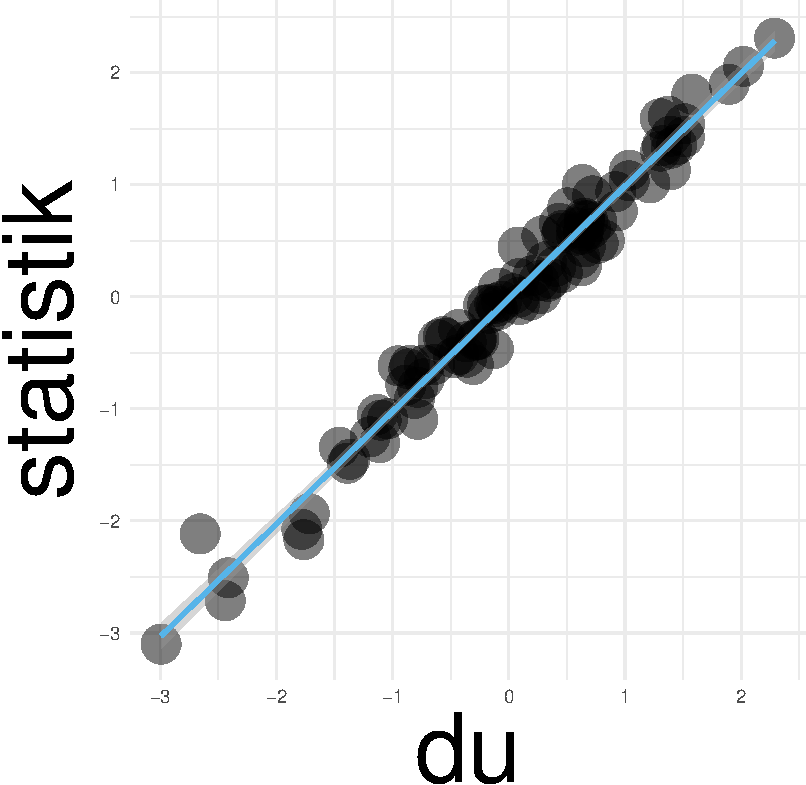
\includegraphics[width=0.33\linewidth,height=\textheight,keepaspectratio]{005-orga_files/figure-pdf/statistik-und-du-guter-fit-1.pdf}

}

\caption{Statistik und Du: Passt!}

\end{figure}%

\section{Es geht um Ihren Lernerfolg}\label{es-geht-um-ihren-lernerfolg}

Meister Yoda rät: Lesen Sie die folgenden Hinweise, s.
Abbildung~\ref{fig-yoda}.

\begin{figure}

\centering{


\includegraphics[width=0.5\linewidth,height=\textheight,keepaspectratio]{img/yoda.jpg}

}

\caption{\label{fig-yoda}Lesen die Inhalte du musst (imgflip, 2024c).}

\end{figure}%

\subsection{Lernziele}\label{lernziele}

\begin{itemize}
\item
  Die Studentis sind mit wesentlichen Methoden der explorativen
  Datenanalyse vertraut und können diese selbständig anwenden.
\item
  Die Studentis können gängige Forschungsfragen in lineare Modelle
  übersetzen, diese auf echte Datensätze anwenden und die Ergebnisse
  interpretieren.
\end{itemize}

\subsection{Was lerne ich hier und wozu ist das
gut?}\label{was-lerne-ich-hier-und-wozu-ist-das-gut}

\emph{Was lerne ich hier?}

Sie lernen das \emph{Handwerk der Datenanalyse} mit einem Schwerpunkt
auf Vorhersage. Anders gesagt: Sie lernen, \emph{Daten aufzubereiten}
und aus Daten \emph{Vorhersagen} abzuleiten. Zum Beispiel: Kommt ein
Student zu Ihnen und sagt \enquote{Ich habe 42 Stunden für die Klausur
gelernt, welche Note kann ich in der Klausur erwarten?}. Darauf Ihre
Antwort: \enquote{Auf Basis meiner Daten und meines Modells müsstest du
eine 2.7 schreiben!} Außerdem lernen Sie, wie man die Güte einer
Vorhersage auf Stichhaltigkeit prüft. Denn Vorhersagen kann man ja in
jeder Eckkneipe oder beim Wahrsager bekommen. Wir wollen aber belastbare
Vorhersagen und wollen zumindest wissen, wie gut die Vorhersagen bisher
waren.

\emph{Warum ist das wichtig?}

Wir wollen nicht auf Leuten vertrauen, die behaupten, sie wüssten, was
für uns gut ist. Wir wollen selber die Fakten beurteilen können.

\emph{Wozu brauche ich das im Job?}

Datenanalyse spielt bereits heute in vielen Berufen eine Rolle. Tendenz
stark zunehmend.

\emph{Wozu brauche ich das im Studium?}

In Forschungsarbeiten (wie in empirischen Forschungsprojekten, etwa in
der Abschlussarbeit) ist es üblich, statistische Ergebnisse hinsichtlich
quantitativ zu analysieren.

\emph{Ist Statistik nicht sehr abstrakt?}

Der Schwerpunkt dieses Kurses liegt auf Anwenden und Tun; ähnlich dem
Erlernen eines Handwerks. Theorien und Abstraktionen stehen nur am Rand.

\emph{Gibt es auch gute Jobs, wenn man sich mit Daten auskennt?}

Das World Economic Forum (2020) berichtet zu den \enquote{Top 20 job
roles in increasing and decreasing demand across industries} (S. 30,
Abb. 22):

\begin{enumerate}
\def\labelenumi{\arabic{enumi}.}
\tightlist
\item
  Data Analysts und Scientists
\item
  AI and Machine Learning Specialists
\item
  Big Data Specialists
\end{enumerate}

\subsection{Was ist hier das
Erfolgsgeheimnis?}\label{was-ist-hier-das-erfolgsgeheimnis}

Das Lesen einer Schwimmfibel nutzt wenig, wenn Sie Freischwimmer werden
wollen. Es hilft nichts: Rein in die Fluten! Wenn das Wasser nicht tief
ist und man jederzeit im Trockenen Pause machen kann, steht Ihrem
Fortschritt beim Lernen nichts im Weg. Ich gebe zu, der Vergleich ist
nicht gerade subtil. Aber es ist so: Sie lernen durch Tun (Lovett \&
Greenhouse, 2000). Dieses Buch bietet dafür reichhaltige Gelegenheit.
Nutzen Sie sie. Jedes Kapitel führt am Ende eine Reihe von Aufgaben auf,
alle mit Lösungen. So können Sie Ihren Lernfortschritt testen. Dass
Schwierigkeiten auftreten, wenn man etwas Neues lernt, ist normal. Das
geht fast allen so. Ihren Lernerfolg kann nur eine Sache gefährden: Wenn
Sie aufgeben. Bleiben Sie dran, und der Erfolg wird sich einstellen!
Abbildung~\ref{fig-lernen} zeigt Daten von \(n=1646\) Studentis, die
zeigen, dass regelmäßiges Üben und Dranbleiben mit Erfolg einhergeht
(Sauer, 2017).

\emph{Dran bleiben} ist der Schlüssel zum Erfolg. Üben Sie regelmäßig.
Geben Sie bei Schwierigkeiten nicht auf. \emoji{person-lifting-weights}
\emoji{clockwise-vertical-arrows} \emoji{key} \emoji{glowing-star}

\begin{figure}

\centering{

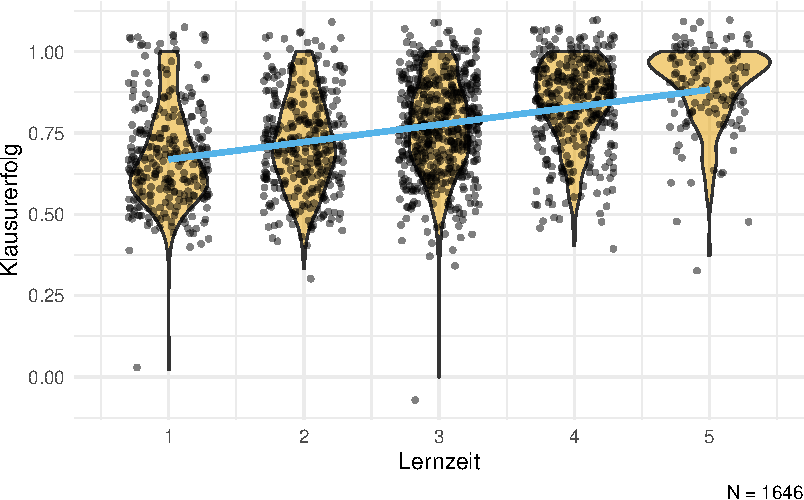
\includegraphics[width=1\linewidth,height=\textheight,keepaspectratio]{005-orga_files/figure-pdf/fig-lernen-1.pdf}

}

\caption{\label{fig-lernen}Der Zusammenhang von Lernzeit (1: gering bis
5:hoch) von Klausurerfolg}

\end{figure}%

\begin{figure}

\begin{minipage}{0.80\linewidth}
Motivation nötig? Dann schauen Sie sich das Video mit einer
\href{https://youtu.be/jtNlzpcPr5Y}{Ansprache zur Motivation}
an.\end{minipage}%
%
\begin{minipage}{0.20\linewidth}

\begin{center}

\includegraphics[width=0.75\linewidth,height=\textheight,keepaspectratio]{005-orga_files/figure-pdf/unnamed-chunk-2-1.pdf}
\end{center}

\end{minipage}%

\end{figure}%

\subsection{Voraussetzungen}\label{voraussetzungen}

Um von diesem Kurs am besten zu profitieren, sollten Sie Folgendes
mitbringen:

\begin{itemize}
\tightlist
\item
  Bereitschaft, Neues zu lernen
\item
  Bereitschaft, bei Schwierigkeiten nicht gleich aufzugeben
\item
  Kenntnis grundlegender Methoden wissenschaftlichen Arbeitens
\end{itemize}

Was Sie \emph{nicht} brauchen, sind besondere Mathe- oder
Statistik-Vorkenntnisse.

\subsection{Überblick über das
Buch}\label{uxfcberblick-uxfcber-das-buch}

Abb. Abbildung~\ref{fig-ueberblick} gibt einen Überblick über den
Verlauf und die Inhalte des Buches. Das Diagramm hilft Ihnen, zu
verorten, wo welches Thema im Gesamtzusammenhang steht.

\begin{figure}

\centering{

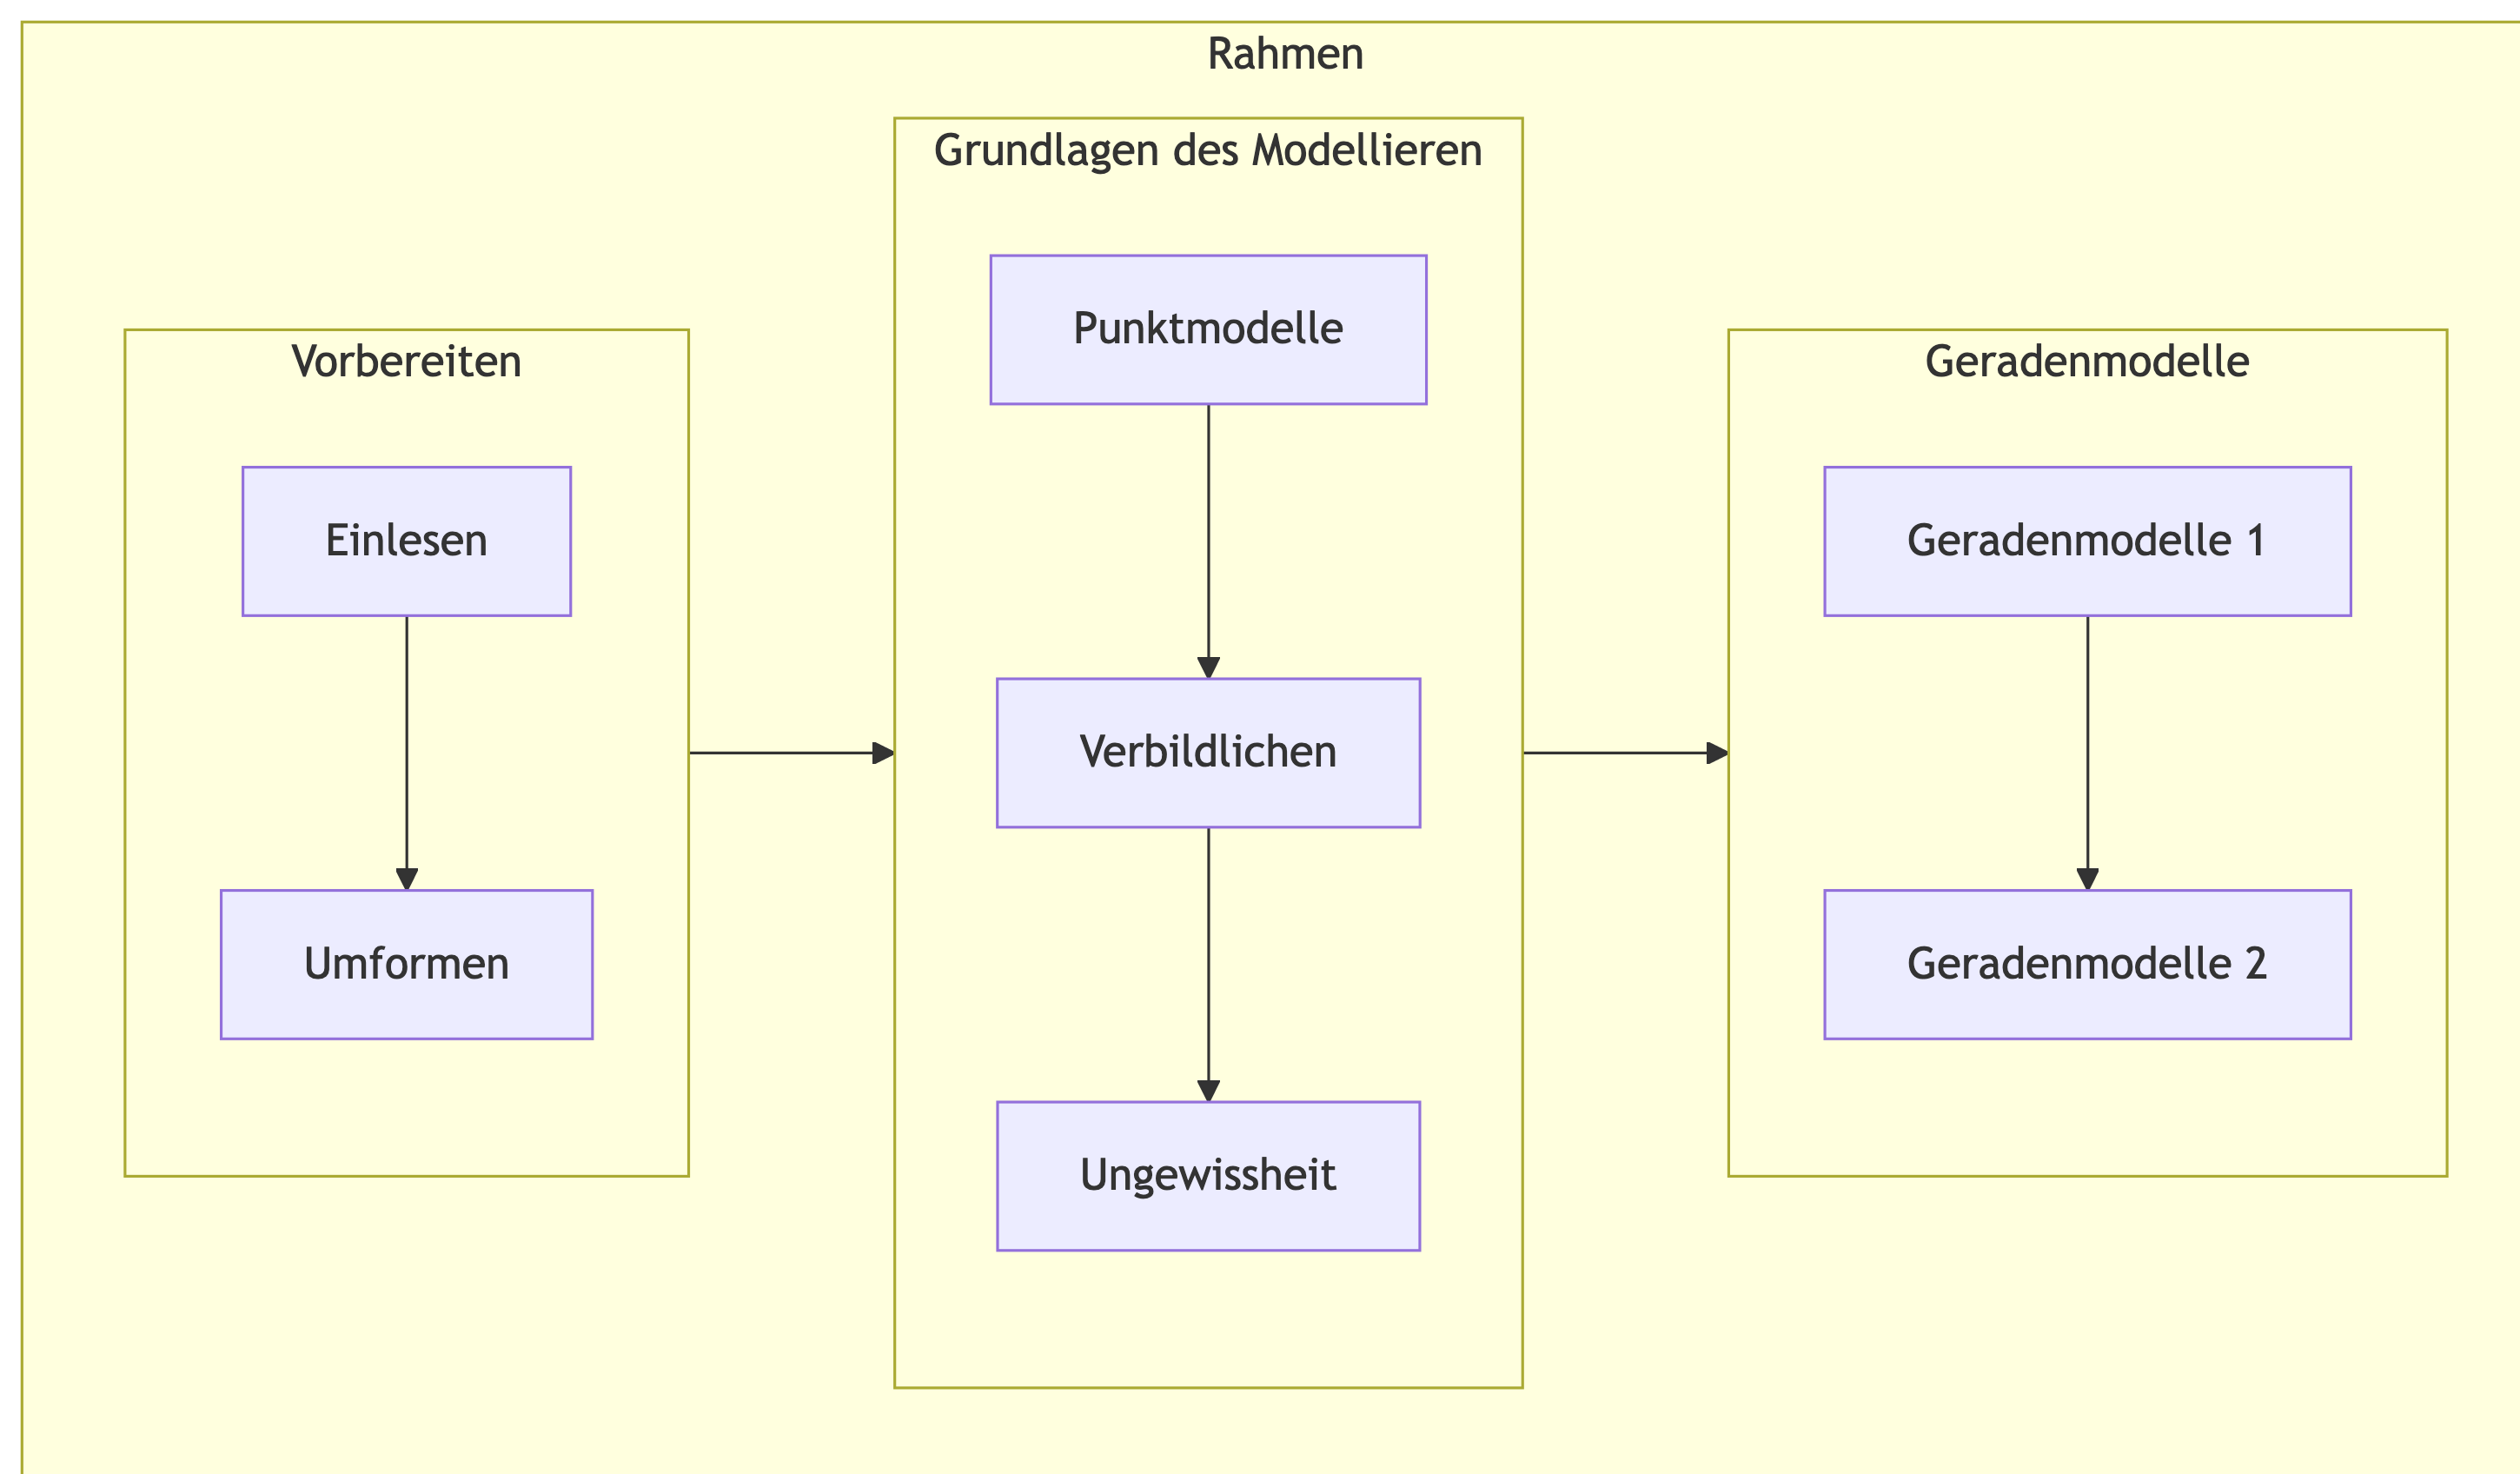
\includegraphics[width=4in,height=2.34in]{005-orga_files/figure-latex/mermaid-figure-1.png}

}

\caption{\label{fig-ueberblick}Überblick über den Inhalt und Verlauf des
Buches}

\end{figure}%

Das Diagramm zeigt auch den Ablauf einer typischen Datenanalyse.
Natürlich kann man sich auch andere sinnvolle Darstellungen dieses
Ablaufs vorstellen.

\section{Lernhilfen}\label{lernhilfen}

Auf der Webseite
\href{https://sebastiansauer.github.io/Datenwerk/}{\enquote{Datenwerk}}
wird eine große Zahl an Aufgaben bereitgestellt.\footnote{\url{https://sebastiansauer.github.io/Datenwerk/}}

\begin{figure}

\begin{minipage}{0.80\linewidth}
Am Ende jedes Kapitels dieses Buchs finden Sie eine Auswahl an
Aufgabennamen, die Sie im Datenwerk finden. Beachten Sie die
\href{https://sebastiansauer.github.io/Datenwerk/hinweise}{Hinweise zu
den Aufgaben}.\end{minipage}%
%
\begin{minipage}{0.20\linewidth}

\begin{center}

\includegraphics[width=0.75\linewidth,height=\textheight,keepaspectratio]{005-orga_files/figure-pdf/unnamed-chunk-4-1.pdf}
\end{center}

\end{minipage}%

\end{figure}%

Außerdem tauchen \emph{im Verlauf jedes Kapitels Übungsaufgaben} an
verschiedenen Stellen auf, so dass Sie den jeweiligen Stoff sofort üben
und Ihr Verständnis prüfen können. Im Buch finden sich mehrere Arten von
\emph{Hervorhebungen}, wie Beispiele, Fehlerquellen, Definitionen und
Hinweise (und verlinkt), sodass Sie schnell finden können, wonach Sie
suchen. Das Buch verweist auf eine Reihe von \emph{Online-Materialien}.
So ist der gesamte R-Code für dieses Buch auf dem Github-Repo dieses
Buches zu finden: \url{https://github.com/sebastiansauer/statistik1}.

\begin{figure}

\begin{minipage}{0.80\linewidth}
Schauen Sie sich mal den YouTube-Kanal \emph{sebastiansauerstatistics}
an und dort die
\href{https://www.youtube.com/playlist?list=PLRR4REmBgpIEaIyeNBgNGPgmhQJ_T1y8_}{Playlist
\enquote{R}}. Dort finden Sie \emph{Videos zum Thema dieses
Buches}.\end{minipage}%
%
\begin{minipage}{0.20\linewidth}

\begin{center}

\includegraphics[width=0.75\linewidth,height=\textheight,keepaspectratio]{005-orga_files/figure-pdf/unnamed-chunk-5-1.pdf}
\end{center}

\end{minipage}%

\end{figure}%

\section{Software}\label{software}

\subsection{R}\label{r}

Sie benötigen R, RStudio und einige R-Pakete für diesen Kurs. Dieses
Buch enthält \enquote{mittel} viel R. Auf fortgeschrittene R-Techniken
wurde aber komplett verzichtet. Dem einen Anfänger oder der anderen
Anfängerin mag es dennoch als \enquote{viel Code} erscheinen. Es wäre ja
auch möglich gewesen, auf R zu verzichten und stattdessen eine
\enquote{Klick-Software} zu verwenden.
\href{https://jasp-stats.org/}{JASP} oder
\href{https://www.jamovi.org/}{Jamovi} sind Beispiele für tolle Software
aus dieser Kategorie. Ich glaube aber, der Verzicht auf eine
Skriptsprache (R) wäre ein schlechter Dienst an den Studentis. Mit Blick
auf eine \enquote{High-Tech-Zukunft} sollte man zumindest mit etwas
Computer-Code vertraut sein. Auf Computercode zu verzichten, erschiene
mir daher fahrlässig für die \enquote{Zukunftsfestigkeit} der
Ausbildung.

Sie finden den R-Code für jedes Kapitel
\href{https://github.com/sebastiansauer/statistik1/tree/main/R-code-for-all-chapters}{im
Github-Repositorium dieses Buches}.\footnote{\url{https://github.com/sebastiansauer/statistik1/tree/main/R-code-for-all-chapters}}

\subsection{R-Pakete}\label{sec-rpckgs}

In den meisten Kapiteln dieses Buches benötigen Sie die folgenden zwei
R-Pakete: \texttt{tidyverse} und \texttt{easystats}.

\begin{Shaded}
\begin{Highlighting}[]
\FunctionTok{library}\NormalTok{(tidyverse)}
\FunctionTok{library}\NormalTok{(easystats)}
\end{Highlighting}
\end{Shaded}

Weitere Hinweise zu R finden Sie in Kapitel~\ref{sec-dateneinlesen}.

\section{Benötigte Daten}\label{benuxf6tigte-daten}

In den meisten Kapiteln dieses Buches analysieren wir Datensätze; meist
ist das der Datensatz \texttt{mariokart}, wo Auktionen zu diesem
Computerspiel in einigen Merkmalen aufgeführt sind. Sie können den
Datensatz auf folgende Art importieren, s.
Listing~\ref{lst-import-mario}.

\begin{codelisting}

\caption{\label{lst-import-mario}Mariokart-Datensatz importieren}

\centering{

\begin{Shaded}
\begin{Highlighting}[]
\NormalTok{mariokart }\OtherTok{\textless{}{-}} \FunctionTok{paste0}\NormalTok{(}
  \StringTok{"https://vincentarelbundock.github.io/Rdatasets/"}\NormalTok{,}
  \StringTok{"csv/openintro/mariokart.csv"}\NormalTok{)}

\NormalTok{mariokart }\OtherTok{\textless{}{-}} \FunctionTok{read.csv}\NormalTok{(mariokart\_path)}
\end{Highlighting}
\end{Shaded}

}

\end{codelisting}%

Ein Data-Dictionary (Codebook) finden Sie in Anhang~\ref{sec-data-dict}.

\part{Vorbereiten}

\chapter{Rahmen}\label{rahmen}

\[
\definecolor{ycol}{RGB}{230,159,0}
\definecolor{modelcol}{RGB}{86,180,233}
\definecolor{errorcol}{RGB}{0,158,115}
\definecolor{beta0col}{RGB}{213,94,0}
\definecolor{beta1col}{RGB}{0,114,178}
\definecolor{xcol}{RGB}{204,121,167}
\]

\section{Einstieg}\label{einstieg}

Abbildung~\ref{fig-ueberblick} zeigt den Standort dieses Kapitels im
Lernpfad und gibt damit einen Überblick über das Thema dieses Kapitels
im Kontext aller Kapitel. Abbildung~\ref{fig-tidy5} zeigt, dass unser
Vorgehen in diesem Buch einem Fließband gleicht: Schritt für Schritt, in
der richtigen Reihenfolge, vom Anfang bis Ende, erarbeiten wir unser
\enquote{Datenprodukt}.

\begin{figure}

\centering{

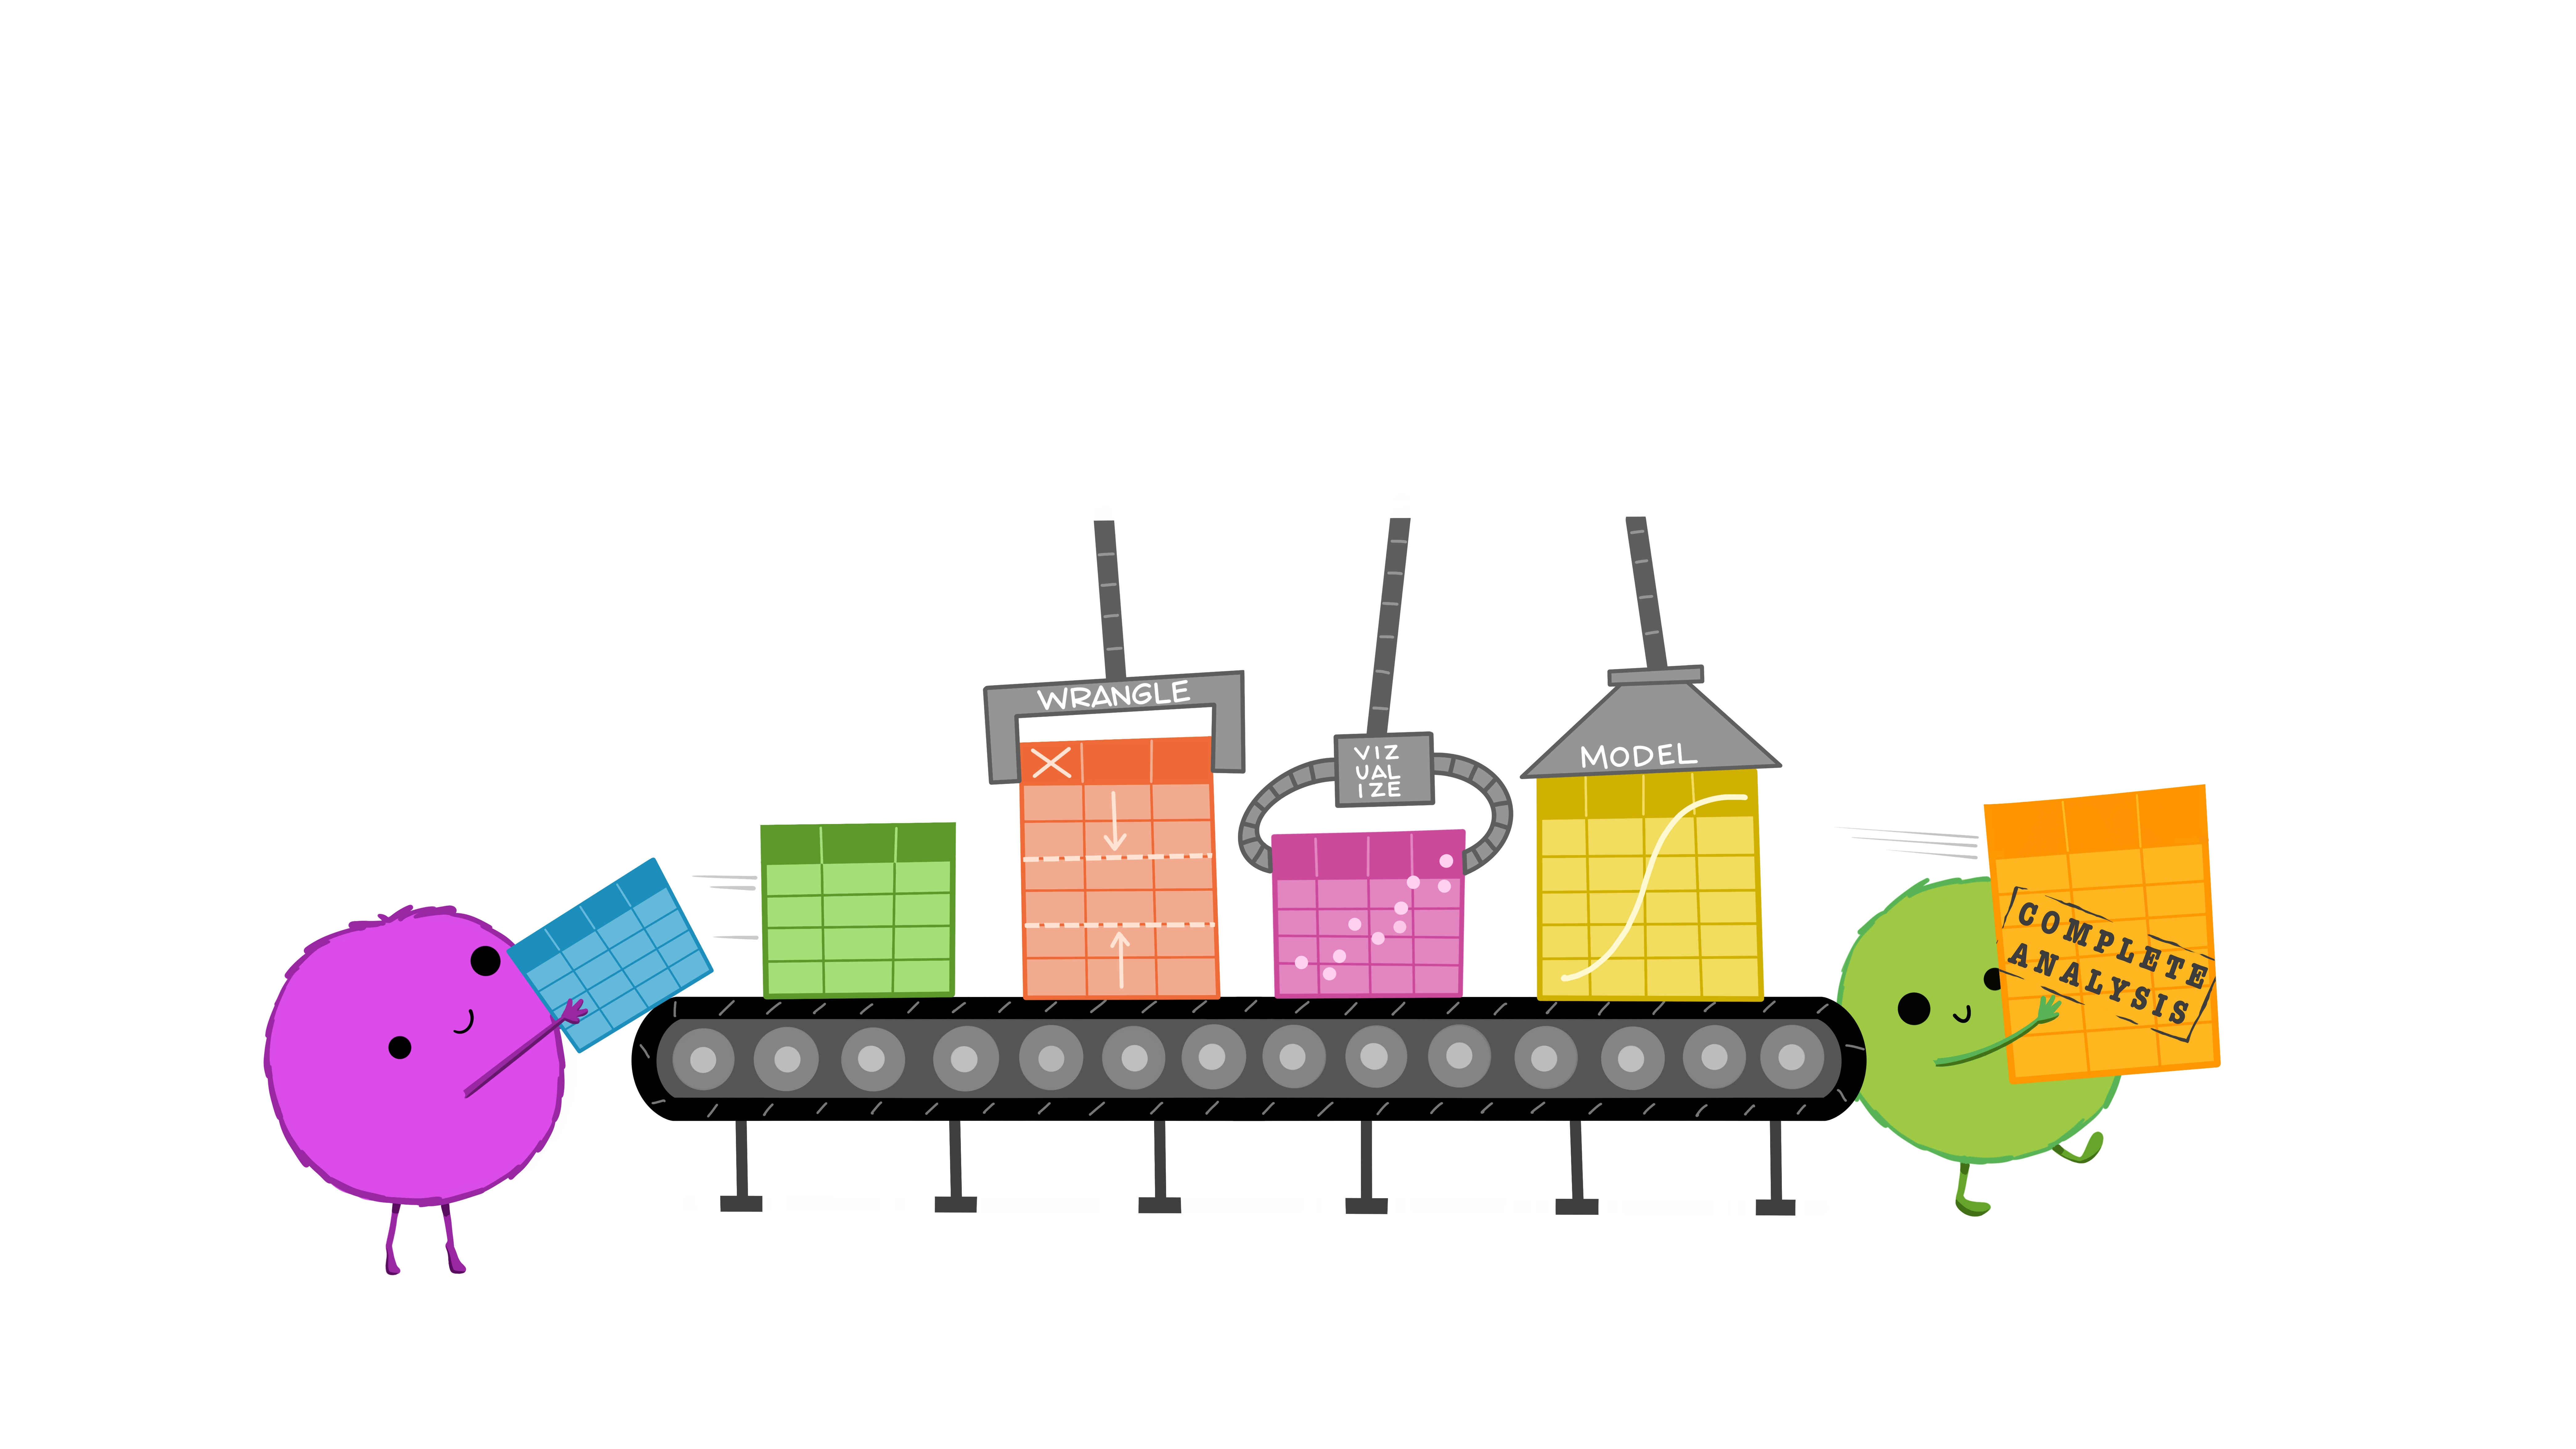
\includegraphics[width=0.75\linewidth,height=\textheight,keepaspectratio]{img/tidydata_5.jpg}

}

\caption{\label{fig-tidy5}Datenanalyse als eine Abfolge am Fließband
(Horst, 2024)}

\end{figure}%

\subsection{Lernziele}\label{lernziele-1}

\begin{itemize}
\tightlist
\item
  Sie können eine Definition von Statistik wiedergeben.
\item
  Sie können eine Definition von Daten wiedergeben.
\item
  Sie können den Begriff Tidy-Daten erläutern.
\item
  Sie können Beispiele für verschiedene Skalenniveaus nennen.
\end{itemize}

\subsection{Erfolgsgrezept}\label{erfolgsgrezept}

Drei Faktoren beeinflussen Ihren Lernerfolg: 1) Ihrer Lehrkraft, 2)
Ihrer Mitarbeit im Unterricht und 3) Ihrem Eigenstudium zuhause (Vor-
bzw. Nachbereitung des Unterrichts), s.
Abbildung~\ref{fig-erfolgsrezept}.

\begin{figure}

\centering{

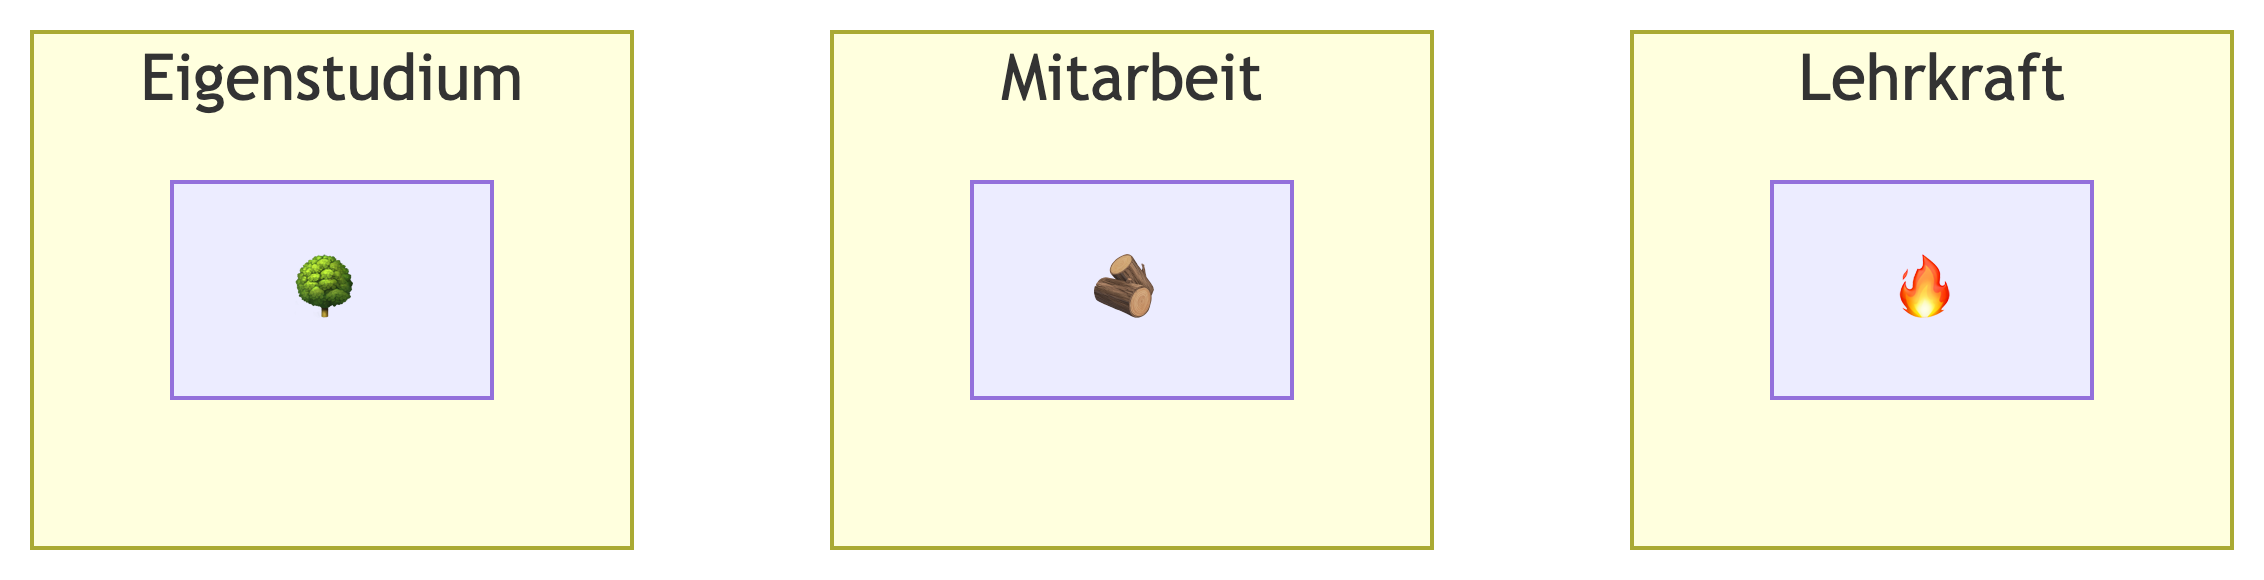
\includegraphics[width=4in,height=1.05in]{010-rahmen_files/figure-latex/mermaid-figure-1.png}

}

\caption{\label{fig-erfolgsrezept}Ihr Lernerfolg besteht aus drei
Komponenten: Der Lehrkraft, Ihrer Mitarbeit im Unterricht und Ihrem
Eigenstudium, d.h. Ihrer Vor- bzw. Nachbereitung zuhause.}

\end{figure}%

Eine gute Lehrkraft ist wie der Funke, der eine (Lern-)Flamme entzündet.
Aber es braucht Brennmaterial, einen Holzscheit, das ist Ihre
Konzentration im Unterricht. Ein Holzscheit allein reicht nicht aus; es
braucht mehr Brennmaterial, um das Feuer am Leben zu erhalten: Ihr
Eigenstudium, das stetige, selbständige Beschäftigen mit der Materie.

\section{Was ist Statistik und wozu ist sie
gut?}\label{was-ist-statistik-und-wozu-ist-sie-gut}

In diesem Buch werden die Begriffe \emph{Statistik}, \emph{Datenanalyse}
und \emph{Data Science} synonym verwendet.

\begin{exercise}[Nutzen von
Statistik]\protect\hypertarget{exr-nutzen-statistik}{}\label{exr-nutzen-statistik}

Fragen Sie einen Chatbot (wie ChatGPT), was der Nutzen von Statistik
ist. Diskutieren Sie die Antwort. \(\square\)

\end{exercise}

Fragen wir doch einen Chatbot wie ChatGPT, was er unter Statistik
versteht:

\begin{quote}
{\emoji{student}} Was ist Statistik? Bitte definiere verständlich.
\end{quote}

\begin{quote}
{\emoji{robot}} Statistik ist eine Wissenschaft, die sich mit der
Sammlung, Analyse, Interpretation, Präsentation und Übertragung von
Daten beschäftigt. Ziel ist es, Muster und Trends in den Daten zu
erkennen und verlässliche Schlussfolgerungen über eine größere Gruppe
(z.B. Bevölkerung) auf der Basis einer Stichprobe (Teilmenge) zu
treffen. Die Statistik hilft uns bei der Beantwortung von Fragen, indem
sie uns dabei hilft, die Unsicherheit in den Daten zu messen und zu
verstehen\footnote{Release 2023-Jan}.
\end{quote}

Es gibt mehrere Definition von Statistik. Hier ist eine, s.
Definition~\ref{def-statistik}.

\begin{definition}[Statistik]\protect\hypertarget{def-statistik}{}\label{def-statistik}

Statistik fasst Werte zusammen, quantifiziert deren Unterschiedlichkeit
und beschreibt die Ungewissheit unserer Schlüsse (Kaplan, 2009;
Poldrack, 2023) . \(\square\)

\end{definition}

Betrachten wir die drei Bestimmungsstücke einer Definition von Statistik
genauer: 1. Daten zusammenfassen, 2. Unterschiedlichkeit quantifizieren
und 3. Ungewissheit beschreiben.

\subsection{Daten zusammenfassen}\label{daten-zusammenfassen}

Abbildung~\ref{fig-zsmnfassen} verdeutlicht das Prinzip des
Zusammenfassens von Daten. Einfach ausgedrückt: Eine Menge von Zahlen
wird zu einer einzelnen Zahl \enquote{zusammengedampft}. Eine einzelne
Zahl ist wesentlich besser zu verstehen als eine große Menge von Zahlen.
Bei vielen Zahlen würde man den Überblick verlieren.

\begin{figure}

\begin{minipage}{0.45\linewidth}

\centering{

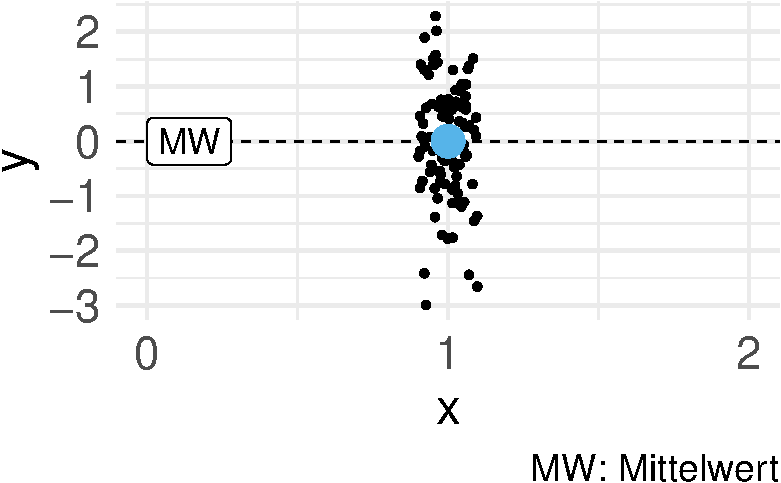
\includegraphics[width=1\linewidth,height=\textheight,keepaspectratio]{010-rahmen_files/figure-pdf/fig-zsmnfassen-1.pdf}

}

\subcaption{\label{fig-zsmnfassen-1}Zusammengefasst zu einem Punkt}

\end{minipage}%
%
\begin{minipage}{0.10\linewidth}
~\end{minipage}%
%
\begin{minipage}{0.45\linewidth}

\centering{

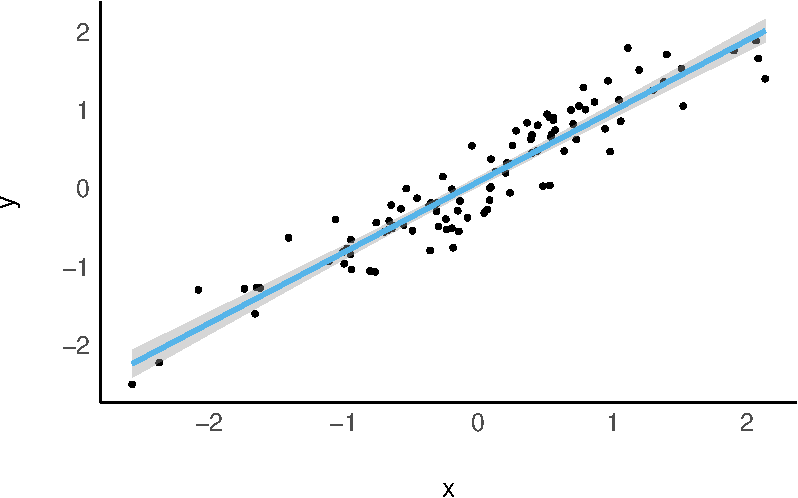
\includegraphics[width=1\linewidth,height=\textheight,keepaspectratio]{010-rahmen_files/figure-pdf/fig-zsmnfassen-2.pdf}

}

\subcaption{\label{fig-zsmnfassen-2}Zusammengefasst zu einer Geraden}

\end{minipage}%

\caption{\label{fig-zsmnfassen}Daten zusammenfassen. (a) Zusammenfassen
einer Variable zu einem Punktwert, hier zum Mittelwert. (b)
Zusammenfassen zweier Variablen zu einer Geraden.}

\end{figure}%

\subsection{Unterschiedlichkeit
quantifizieren}\label{unterschiedlichkeit-quantifizieren}

Eine allgegenwärtige Tatsache ist, dass die Dinge der Welt sich
unterscheiden, etwa, dass Exemplare einer Gattung sich unterscheiden. So
sind nicht alle Menschen gleich groß, nicht alle Bücher gleich lang oder
nicht alle Tage gleich warm.

Ein zentrales Vorgehen bei statistischen Analysen ist es, die
\emph{Unterschiedlichkeit der Dinge} zu beschreiben, präziser gesagt:
die \emph{Variation zu quantifizieren}. Betrachten wir dazu das Beispiel
in Abbildung~\ref{fig-groesse}.

\begin{figure}

\centering{

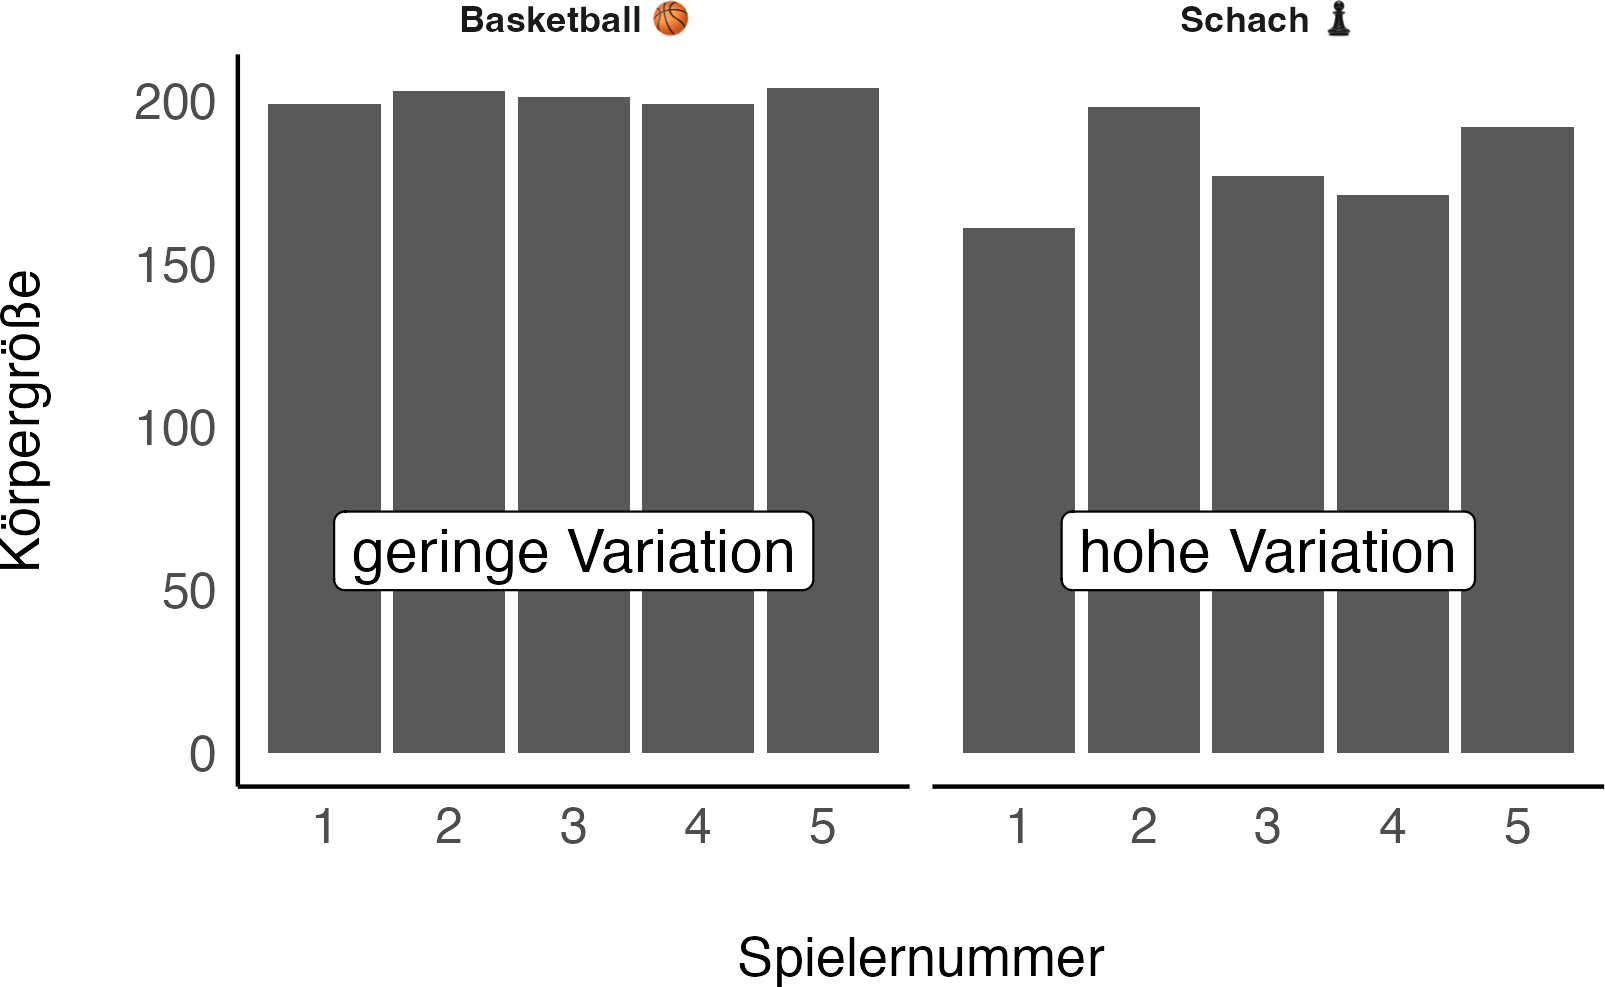
\includegraphics[width=0.75\linewidth,height=\textheight,keepaspectratio]{010-rahmen_files/figure-pdf/fig-groesse-1.png}

}

\caption{\label{fig-groesse}Wenig Variation in der Körpergröße bei den
Basketballern. Alles lange Kerle. Viel Variation bei den Schachspielern:
Manche sind klein, ander groß.}

\end{figure}%

Bei den Basketballern gibt es \emph{geringe} Variation in der
Körpergröße -- alle sind groß, ähnlich groß. Bei den Schachspielern gibt
es (im Verhältnis) \emph{hohe} Variation: Einige Personen sind groß,
andere klein.

Eine \emph{Abweichung} (auch \emph{Residuum}) genannt, zeigt hier die
Differenz von Mittelwert und dem Wert der Körpergröße bei der jeweiligen
Person. Nehmen wir an, wir sprechen allgemein von einer Person \(i\).
Wir bezeichnen das Merkmal Körpergröße mit \(X\) und den Mittelwert der
Körpergröße mit als \(\bar{x}\) (\enquote{x quer}). Dann können wir kdas
Residuum der \(i\)-ten Person mit \(r_i\) bezeichnen und entsprechend
definieren.

\begin{definition}[Residuum]\protect\hypertarget{def-residuum}{}\label{def-residuum}

Das Residuum des Merkmals \(X\) der \(i\)-ten Beobachtung ist definiert
als die Differenz vom Wert \(x_i\) und einem Referenzwert, etwa dem
Mittelwert (\(\bar{x}\)), d.h.: \(r_i = x_i - \bar{x}.\square\)

\end{definition}

\subsection{Ungewissheit beschreiben}\label{ungewissheit-beschreiben}

\begin{example}[]\protect\hypertarget{exm-ungewiss1}{}\label{exm-ungewiss1}

Anna hat eine Statistik-Klausur geschrieben. Sie hat keine Ahnung, ob
sie bestehen wird. Berta hingegen ist sich sehr sicher, dass sie
bestanden hat. Die beiden Studentinnen unterscheiden sich also stark in
der Ungewissheit hinsichtlich ihrer Einschätzung zum Klausurerfolg, s.
Abbildung~\ref{fig-ungewiss-anna-berta}. \(\square\)

\end{example}

\begin{figure}

\begin{minipage}{0.50\linewidth}

\centering{

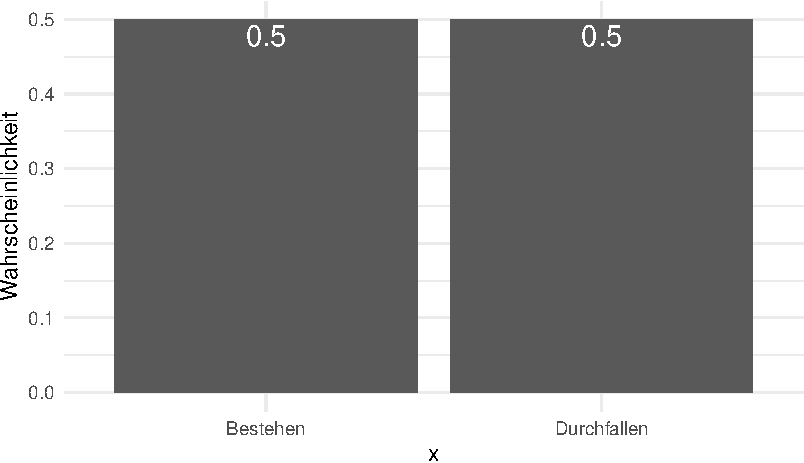
\includegraphics[width=1\linewidth,height=\textheight,keepaspectratio]{010-rahmen_files/figure-pdf/fig-ungewiss-anna-berta-1.pdf}

}

\subcaption{\label{fig-ungewiss-anna-berta-1}Was Anna denkt}

\end{minipage}%
%
\begin{minipage}{0.50\linewidth}

\centering{

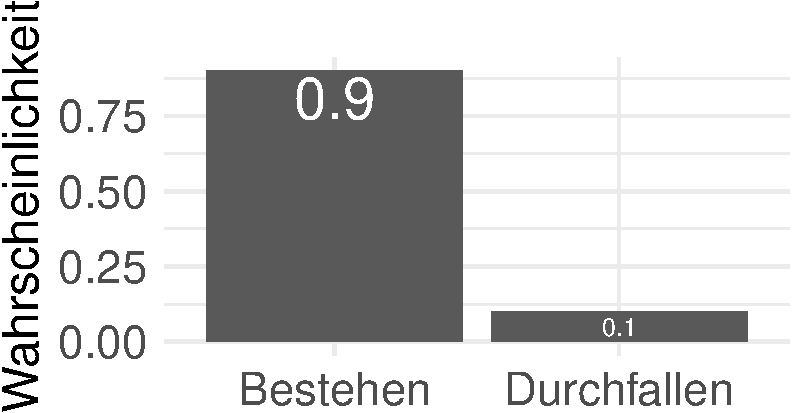
\includegraphics[width=1\linewidth,height=\textheight,keepaspectratio]{010-rahmen_files/figure-pdf/fig-ungewiss-anna-berta-2.pdf}

}

\subcaption{\label{fig-ungewiss-anna-berta-2}Was Berta denkt}

\end{minipage}%

\caption{\label{fig-ungewiss-anna-berta}Die Ungewissheit, die wir
Ereignissen zuschreiben, kann variieren}

\end{figure}%

\begin{example}[]\protect\hypertarget{exm-ungewiss2}{}\label{exm-ungewiss2}

Sagen wir, Sie haben sich mit einem zwielichten Statistiker auf ein
Glücksspiel eingelassen: Er wirft eine Münze 10 Mal; bei Kopf gewinnt
er, bei Zahl sie. Nun hat der Statistiker von den 10 Würfen 8 Mal
gewonnen. \emph{Sie} sind sich \emph{ziemlich} sicher, dass dieser Typ
Sie über den Tisch gezogen hat. Allerdings sind Sie nicht ganz sicher,
und beweisen können Sie es leider auch nicht. \emph{Der zwielichte
Statistiker} ist sich \emph{ganz sicher}: Er weiß, dass er Sie über den
Tisch gezogen hat, er weiß, dass seine Münze gezinkt ist. \(\square\)

\end{example}

\section{Was ist das Ziel Ihrer
Analyse?}\label{was-ist-das-ziel-ihrer-analyse}

\subsection{Arten von Zielen}\label{arten-von-zielen}

Statistische Analysen können drei Arten von Zielen verfolgen, s.
Abbildung~\ref{fig-ziele}.

\begin{figure}

\centering{

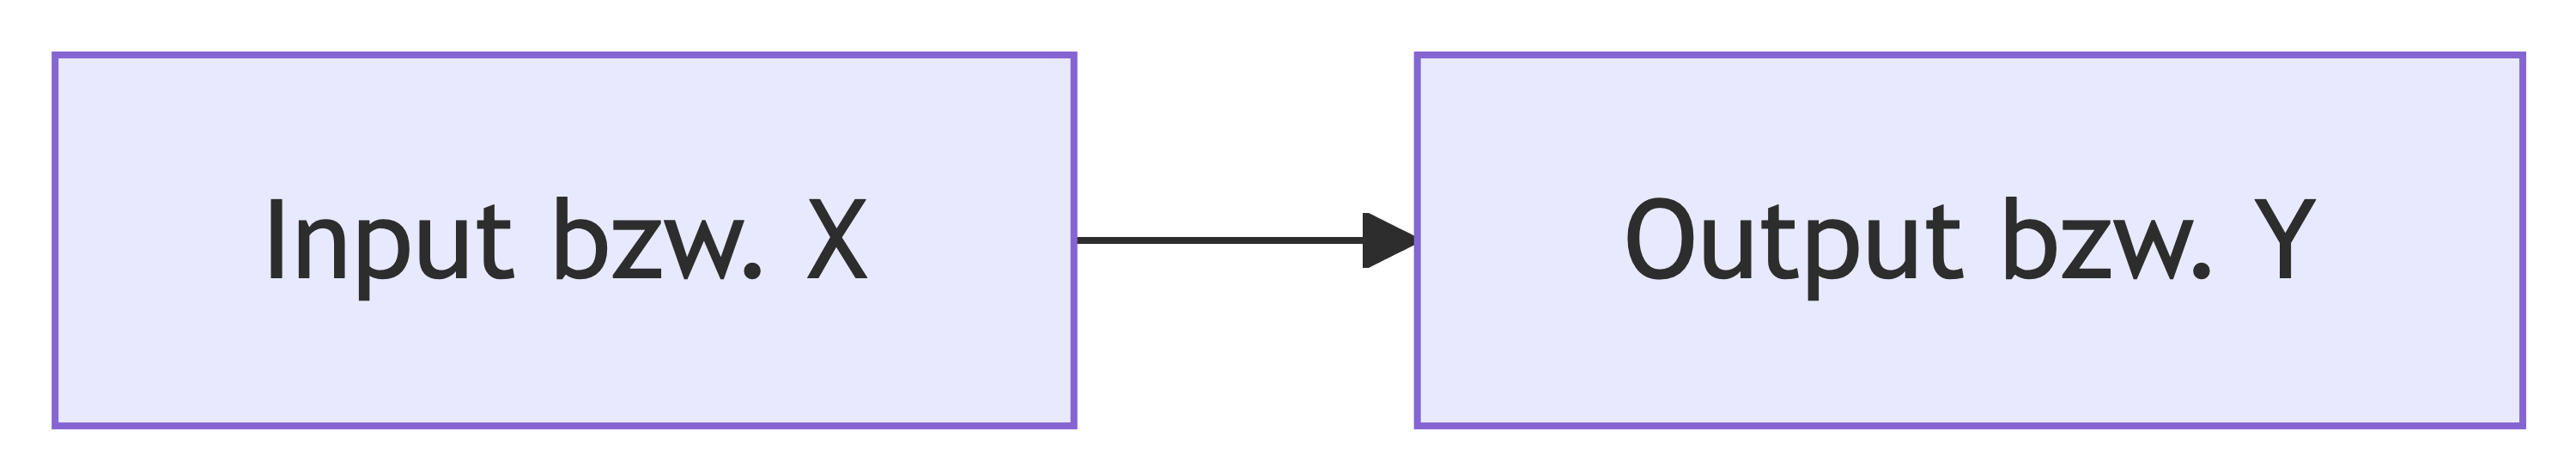
\includegraphics[width=4in,height=0.97in]{010-rahmen_files/figure-latex/mermaid-figure-6.png}

}

\caption{\label{fig-ziele}Zielarten einer Datenanalyse}

\end{figure}%

\begin{example}[]\protect\hypertarget{exm-zielarten}{}\label{exm-zielarten}

~

\begin{itemize}
\tightlist
\item
  \emph{Beschreiben}: Wie groß ist der Gender-Paygap in der Branche X im
  Zeitraum Y?
\item
  \emph{Vorhersagen}: Wenn ich 100 Stunden auf die Statistikklausur
  lernen, welche Note kann ich dann erwarten?
\item
  \emph{Erklären}: Wie viel bringt mir das Lernen auf die
  Statistikklausur? \(\square\)
\end{itemize}

\end{example}

\begin{exercise}[]\protect\hypertarget{exr-ziele-stat}{}\label{exr-ziele-stat}

Benennen Sie Beispiele für die die drei Zielarten von Datenanalysen!
\(\square\)

\end{exercise}

\subsection{Forschungsfrage}\label{forschungsfrage}

Eine Forschungsfrage ist die Leitfrage Ihrer Analyse. Sie definiert, was
Sie herausfinden wollen. Häufig fragen Forschungsfragen: \enquote{Hat X
einen (kausalen) Einfluss auf Y?}

Eine Forschungsfrage weist häufig folgende Struktur auf, s.
Abbildung~\ref{fig-fo-struktur}.

\begin{figure}

\centering{

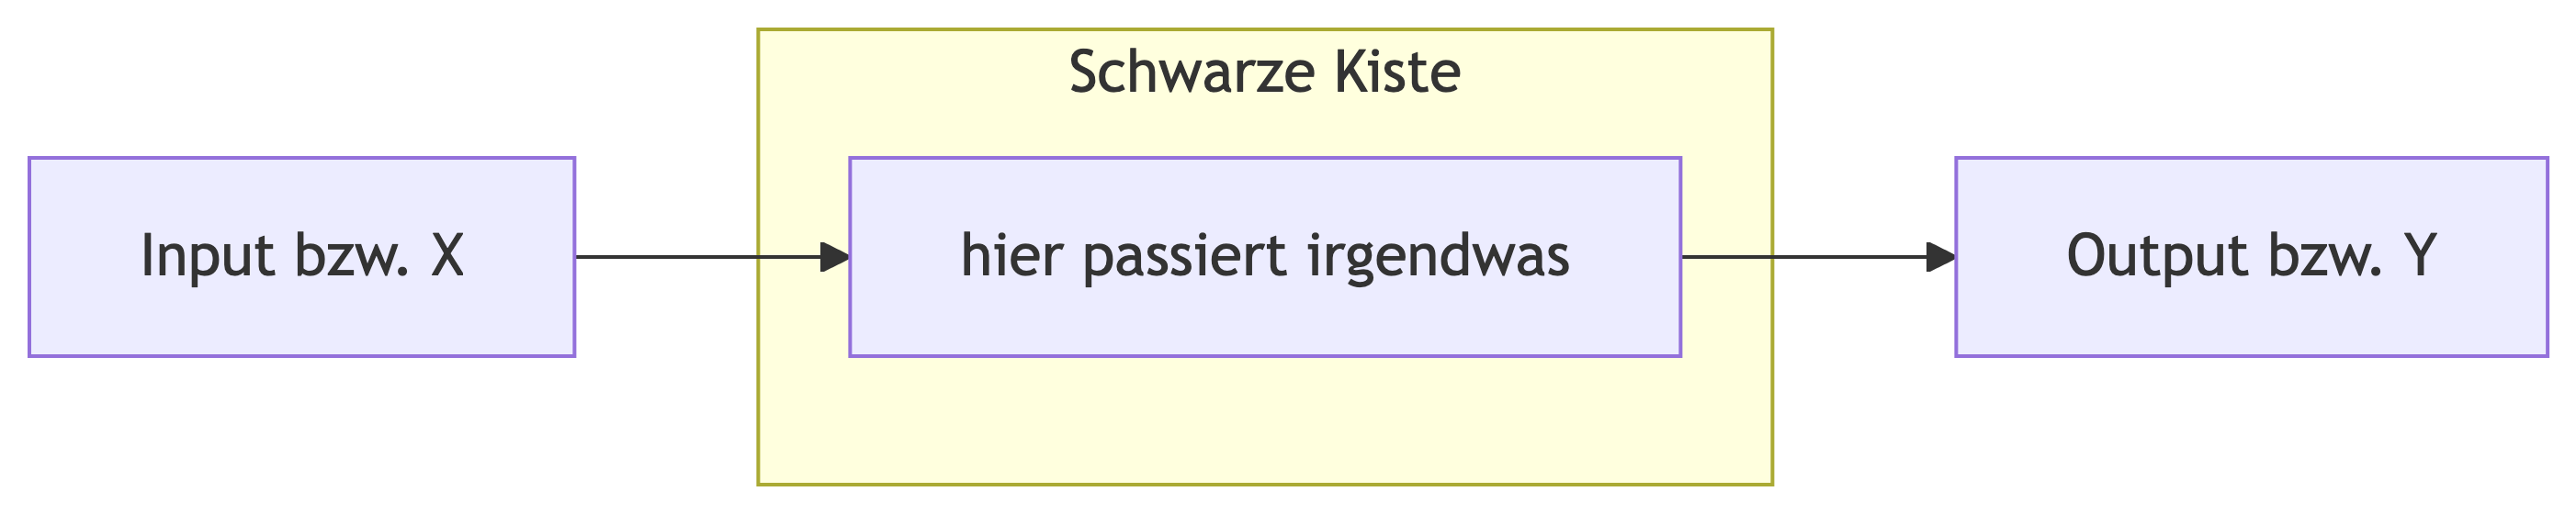
\includegraphics[width=4in,height=0.75in]{010-rahmen_files/figure-latex/mermaid-figure-5.png}

}

\caption{\label{fig-fo-struktur}Struktur eine Forschungsfrage}

\end{figure}%

\begin{example}[Forschungsfragen]\protect\hypertarget{exm-fofrage1}{}\label{exm-fofrage1}

~

\begin{quote}
Hat Lernen (X) einen Einfluss auf den Prüfungserfolg (Y)?
\end{quote}

\begin{quote}
Verringert Joggen (X) die Menge des Hüftgolds (Y)?
\end{quote}

\begin{quote}
Um welchen Betrag erhöht sich der Umsatz (Y), wenn wir 1000 € mehr für
Werbung ausgeben? (X)
\end{quote}

\begin{quote}
Verringert intensive Handynutzung die Konzentrationsfähigkeit?
\(\square\)
\end{quote}

\end{example}

\begin{example}[Forschungsfrage: Produktmerkmale und
Verkaufserlös]\protect\hypertarget{exm-fofrage2}{}\label{exm-fofrage2}

Nach dem Studium haben Sie bei einem großen Online-Auktionshaus
angeheuert. Da Sie angaben, sich im Studium \st{intensiv} etwas mit
Statistik beschäftigt zu haben, hat man Sie in die Abteilung für
Forschung und Entwicklung (F\&E) gesteckt. Heute ist es Ihre Aufgabe,
Auktionen zur Spielekonsole Wii zu analysieren, genauer gesagt geht es
um das Spiel Mariokart. Ihre Forschungsfrage lautet:

\begin{quote}
Welche Produktmerkmale stehen mit einem hohen Verkaufserlös in
Zusammenhang? \(\square\)
\end{quote}

\end{example}

\subsection{Aus der Forschung:
Smartphone-Brain-Drain}\label{aus-der-forschung-smartphone-brain-drain-1}

Ward et al. (2017) untersuchten die Forschungsfrage, ob die bloße
Gegenwart eines Handys (z.B. wenn es vor Ihnen auf dem Tisch liegt) dazu
führt, dass man abgelenkt wird und daher schlechtere kognitive
Leistungen zeigt.

Die Autoren formulieren ihre Hypothese leider nicht explizit, aber sie
lässt sich implizit aus dem Text herauslesen (S. 142):

\begin{quote}
First, smartphones may redirect the orientation of conscious attention
away from the focal task and toward thoughts or behaviors associated
with one's phone. Prior research provides ample evidence that \ldots{}
this digital distraction adversely affects both performance \ldots{} and
enjoyment.
\end{quote}

Später präzisieren sie ihre Hypothese (S. 143):

\begin{quote}
In two experiments, we test the hypothesis that the mere presence of
one's own smartphone reduces available cognitive capacity.
\end{quote}

Die Ergebnisse unterstützen Ihre Hypothese, s.
Abbildung~\ref{fig-braindrain}. Die kognitive Leistung (Y-Achse) ist
sowohl in der Kapazität des Arbeitsgedächtnisses als auch in der fluiden
Intelligenz geringer, wenn das Handy auf dem Schreibtisch liegt, als
wenn es nicht im Raum ist. Am besten ist die kognitive Leistung, wenn
das Handy nicht im Raum ist. \(\square\)

\begin{figure}

\centering{

\pandocbounded{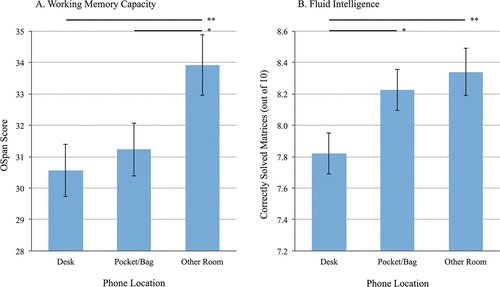
\includegraphics[keepaspectratio]{img/braindrain1.jpg}}

}

\caption{\label{fig-braindrain}Handy in Sichtweite verringert die
kognitiven Ressourcen, Ward et al. (2017), S. 145}

\end{figure}%

\begin{exercise}[]\protect\hypertarget{exr-braindrain-chatgpt}{}\label{exr-braindrain-chatgpt}

Fragen Sie einen Bot (z.B. ChatGPT) zum Stand der Forschung hinsichtlich
der Braindrain-Forschungsfrage. Diskutieren Sie die Antwort, auch in
ihren Grenzen. \(\square\)

\end{exercise}

\subsection{Der Prozess der
Datenanalyse}\label{der-prozess-der-datenanalyse}

Datenanalyse ist eine Art des Problemlösens. Anders gesagt, man macht es
nicht zum Spaß (jedenfalls nicht alle von uns), sondern um ein Ziel zu
erreichen, also ein Problem zu lösen. Daher analysiert man nicht gleich
zu Anfang wild drauf los. Zunächst 1) klärt man das Problem und das
Ziel. Dann 2) plant man das Vorgehen, z.B. welche Daten man erheben
möchte. Als nächstes 3) erhebt man die Daten und bereitet sie auf.
Schließlich kann man sie 4) endlich analysieren. Aber Daten sprechen
nicht für sich, man muss sie 5) interpretieren und Schlüsse daraus
ziehen. Dazu gehört auch, dass man die Schwächen der eigenen Analyse
kritisch beleuchtet, vgl. Abbildung~\ref{fig-ppdac}. Diesen Ablauf nennt
man auch das PPDAC-Modell (MacKay \& Oldford, 2000):

\begin{itemize}
\tightlist
\item
  P: \emph{Problem} (Problem und Ziel und Sachgegenstand verstehen)
\item
  P: \emph{Plan} (Vorgehen planen)
\item
  D: \emph{Data} (Daten erheben und aufbereiten)
\item
  A: \emph{Analysis} (Daten analysieren)
\item
  C: \emph{Conclusions} (Schlussfolgerungen ziehen)
\end{itemize}

\begin{figure}

\centering{

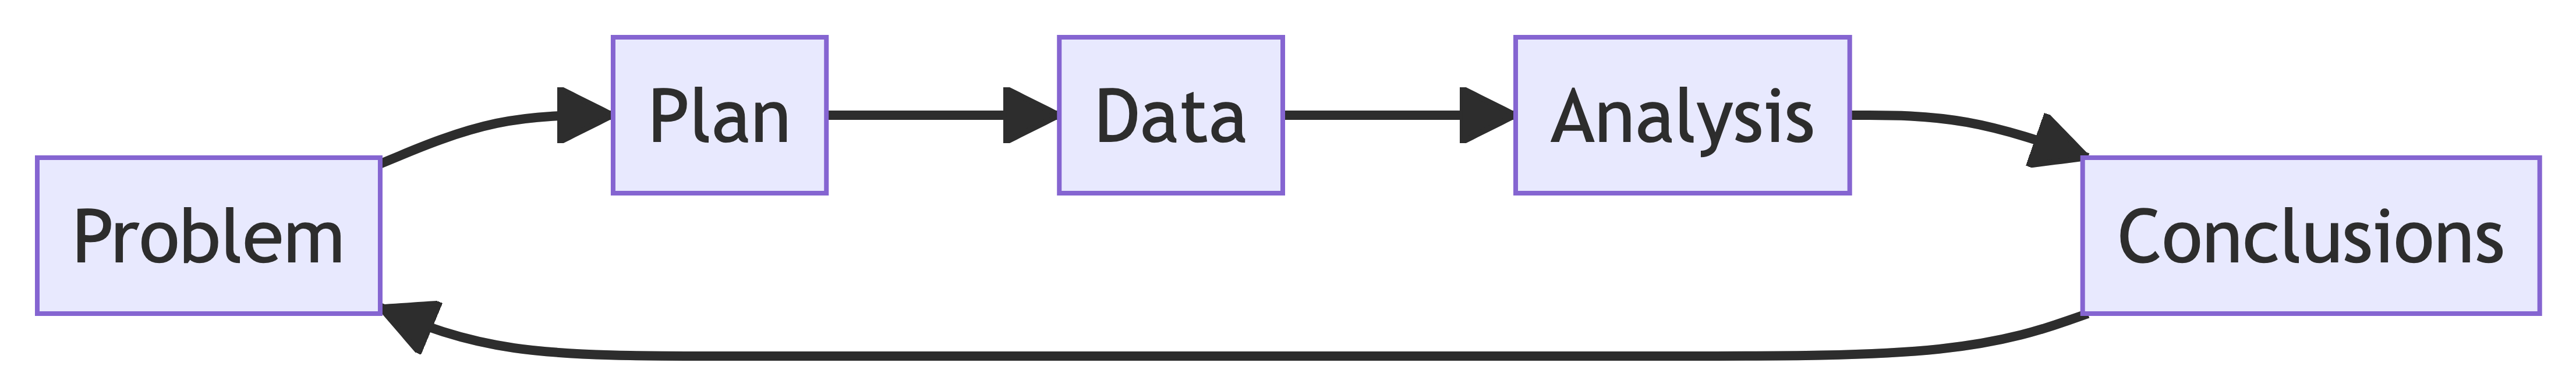
\includegraphics[width=4in,height=0.54in]{010-rahmen_files/figure-latex/mermaid-figure-4.png}

}

\caption{\label{fig-ppdac}Datenanalyse als Prozess: Das PPDAC-Modell}

\end{figure}%

\section{Was sind Daten?}\label{was-sind-daten}

\begin{definition}[Daten]\protect\hypertarget{def-daten}{}\label{def-daten}

Daten sind eine geordnete Folge von Zeichen. \(\square\)

\end{definition}

Tabellen sind oft das geeignetste Format für die Untersuchung von Daten.
Tabelle~\ref{tbl-daten} zeigt ein Beispiel für Daten. Die erste Spalte
\texttt{id} ist nur eine laufende Nummer. Sie dient dazu, die einzelnen
Beobachtungen (hier Studentis) identifizieren zu können und birgt
ansonsten keine Information. Beispiele für ID-Variablen sind z.B.
Matrikelnummer, Personalausweisnummern oder Bestellnummern.

\begin{longtable}[]{@{}rlr@{}}

\caption{\label{tbl-daten}So sehen Daten in Form einer Tabelle aus.}

\tabularnewline

\toprule\noalign{}
id & name & note \\
\midrule\noalign{}
\endhead
\bottomrule\noalign{}
\endlastfoot
1 & Anna & 1.3 \\
2 & Berta & 2.3 \\
3 & Carla & 3.0 \\

\end{longtable}

\begin{example}[Daten zur Forschungsfrage
2]\protect\hypertarget{exm-daten}{}\label{exm-daten}

Hier ist ein Auszug der Daten zur Tabelle \texttt{mariokart}, s.
Tabelle~\ref{tbl-mariokart}.

\begin{longtable}[]{@{}rrrr@{}}

\caption{\label{tbl-mariokart}Auszug aus der Tabelle mariokart}

\tabularnewline

\toprule\noalign{}
n\_bids & start\_pr & total\_pr & wheels \\
\midrule\noalign{}
\endhead
\bottomrule\noalign{}
\endlastfoot
20 & 0.99 & 52 & 1 \\
13 & 0.99 & 37 & 1 \\
16 & 0.99 & 46 & 1 \\
18 & 0.99 & 44 & 1 \\
20 & 0.01 & 71 & 2 \\
19 & 0.99 & 45 & 0 \\

\end{longtable}

Eine Erklärung (Data-Dictionary) aller Variablen des Datensatzes
\texttt{mariokart} findet sich
\href{https://www.openintro.org/data/index.php?data=mariokart}{hier}.\footnote{\url{https://www.openintro.org/data/index.php?data=mariokart}}
\(\square\)

\end{example}

\begin{definition}[Data-Dictionary]\protect\hypertarget{def-datadict}{}\label{def-datadict}

Eine Erklärung, was die Variablen (Spalten) einer Datentabelle bedeuten,
nennt man \emph{Codebook} or \emph{Data-Dictionary}. \(\square\)

\end{definition}

In den Spalten einer Tabelle stehen Merkmale (Variablen) von den Dingen,
die untersucht werden, z.B. Patienten, Kunden oder Videospiele. Die
untersuchten Dinge nennt man Beobachtungseinheiten. Die
Beobachtungseinheiten stehen in den Zeilen einer Tabelle.

\begin{definition}[Variable]\protect\hypertarget{def-var}{}\label{def-var}

Eine Variable ist ein Platzhalter für ein Merkmal, das verschiedene
Ausprägungen annehmen kann. \(\square\)

\end{definition}

Man kann sich eine Variable wie einen Behälter vorstellen, auf dem mit
einem Stift geschrieben steht, was für eine Art Inhalt darin ist, s.
Abbildung~\ref{fig-var-zuweisen}.

\begin{figure}

\centering{

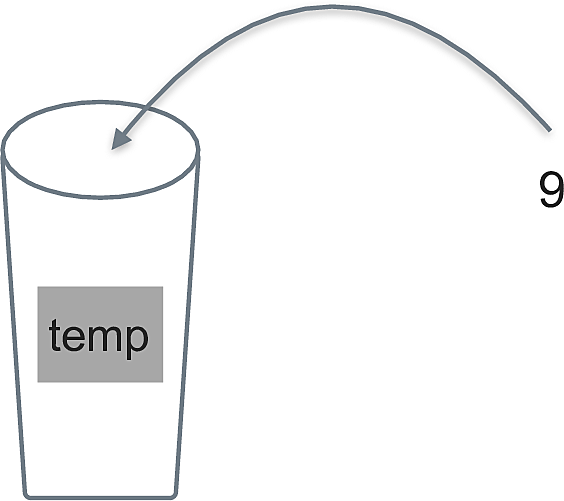
\includegraphics[width=0.25\linewidth,height=\textheight,keepaspectratio]{img/Variablen_zuweisen.png}

}

\caption{\label{fig-var-zuweisen}Wir definieren eine Variable
\enquote{temp} mit dem Inhalt \enquote{9}.}

\end{figure}%

\begin{definition}[Beobachtungseinheit]\protect\hypertarget{def-beobeinheit}{}\label{def-beobeinheit}

Beobachtungseinheiten sind die Dinge, die wir untersuchen (beobachten).
Beobachtungseinheiten sind die Träger von Variablen. \(\square\)

\end{definition}

Tabelle~\ref{tbl-daten} enthält drei Variablen (\texttt{id},
\texttt{Name} und \texttt{Note}) und Note) und drei
Beobachtungseinheiten (\emph{Anna}, \emph{Berta} und \emph{Carla}).
Beobachtungseinheiten werden auch kurz als \emph{Beobachtungen}
bezeichnet.

\begin{definition}[Wert]\protect\hypertarget{def-wert}{}\label{def-wert}

Ein \emph{Wert} ist der Inhalt einer Variablen. \(\square\)

\end{definition}

In Abbildung~\ref{fig-var-zuweisen} ist der Wert von \texttt{temp} 9. In
Tabelle~\ref{tbl-daten} nimmt die Variable \texttt{name} die Werte Anna,
Berta und Carla an.

\begin{definition}[Ausprägung]\protect\hypertarget{def-auspraegung}{}\label{def-auspraegung}

Als \emph{Ausprägungen} bezeichnet man die \emph{verschiedenen} Werte
einer Variablen. \(\square\)

\end{definition}

\begin{example}[]\protect\hypertarget{exm-geschlecht}{}\label{exm-geschlecht}

In einer Studie wurden zehn Probanden untersucht. Die Variable
\texttt{geschlecht} dokumentiert die Geschlechter der Personen:

\begin{Shaded}
\begin{Highlighting}[]
\NormalTok{geschlecht }\OtherTok{\textless{}{-}} \FunctionTok{c}\NormalTok{(}\StringTok{"Mann"}\NormalTok{, }\StringTok{"Frau"}\NormalTok{, }\StringTok{"Frau"}\NormalTok{, }\StringTok{"Frau"}\NormalTok{, }\StringTok{"Mann"}\NormalTok{,}
                \StringTok{"Frau"}\NormalTok{, }\StringTok{"Mann"}\NormalTok{, }\StringTok{"Mann"}\NormalTok{, }\StringTok{"divers"}\NormalTok{, }\StringTok{"Frau"}\NormalTok{)}
\NormalTok{geschlecht}
\DocumentationTok{\#\#  [1] "Mann"   "Frau"   "Frau"   "Frau"   "Mann"   "Frau"   "Mann"   "Mann"  }
\DocumentationTok{\#\#  [9] "divers" "Frau"}
\end{Highlighting}
\end{Shaded}

Die Variable enthält drei Ausprägungen: divers, Frau, Mann. \(\square\)

\end{example}

\begin{tcolorbox}[enhanced jigsaw, leftrule=.75mm, breakable, left=2mm, colback=white, colframe=quarto-callout-tip-color-frame, opacitybacktitle=0.6, coltitle=black, colbacktitle=quarto-callout-tip-color!10!white, arc=.35mm, bottomtitle=1mm, toprule=.15mm, rightrule=.15mm, toptitle=1mm, titlerule=0mm, title=\textcolor{quarto-callout-tip-color}{\faLightbulb}\hspace{0.5em}{Tipp}, bottomrule=.15mm, opacityback=0]

Gerade haben Sie etwas Computer-Syntax gesehen, genauer gesagt, Befehle
aus der Programmiersprache \emph{R}. Bisher haben wir diese Befehle
nicht kennengelernt. Sie verstehen Sie vermutlich (nicht ganz).
Ignorieren Sie diese Befehle einfach erst einmal.

\end{tcolorbox}

\subsection{Tidy Data}\label{tidy-data}

\begin{definition}[Tidy
Data]\protect\hypertarget{def-tidy}{}\label{def-tidy}

Unter \emph{Tidy Data} (tidy data, \enquote{Normalform}) versteht man
eine Tabelle, in der jede Zeile eine Beobachtungseinheit darstellt, jede
Spalte eine Variable und jede Zelle der Tabelle einen Wert, s.
Abbildung~\ref{fig-tidy1}. (Zusätzlich ist noch eine \enquote{Kopfzeile}
erlaubt, in der die Namen der Variablen stehen.) \(\square\)

\end{definition}

\begin{figure}

\centering{

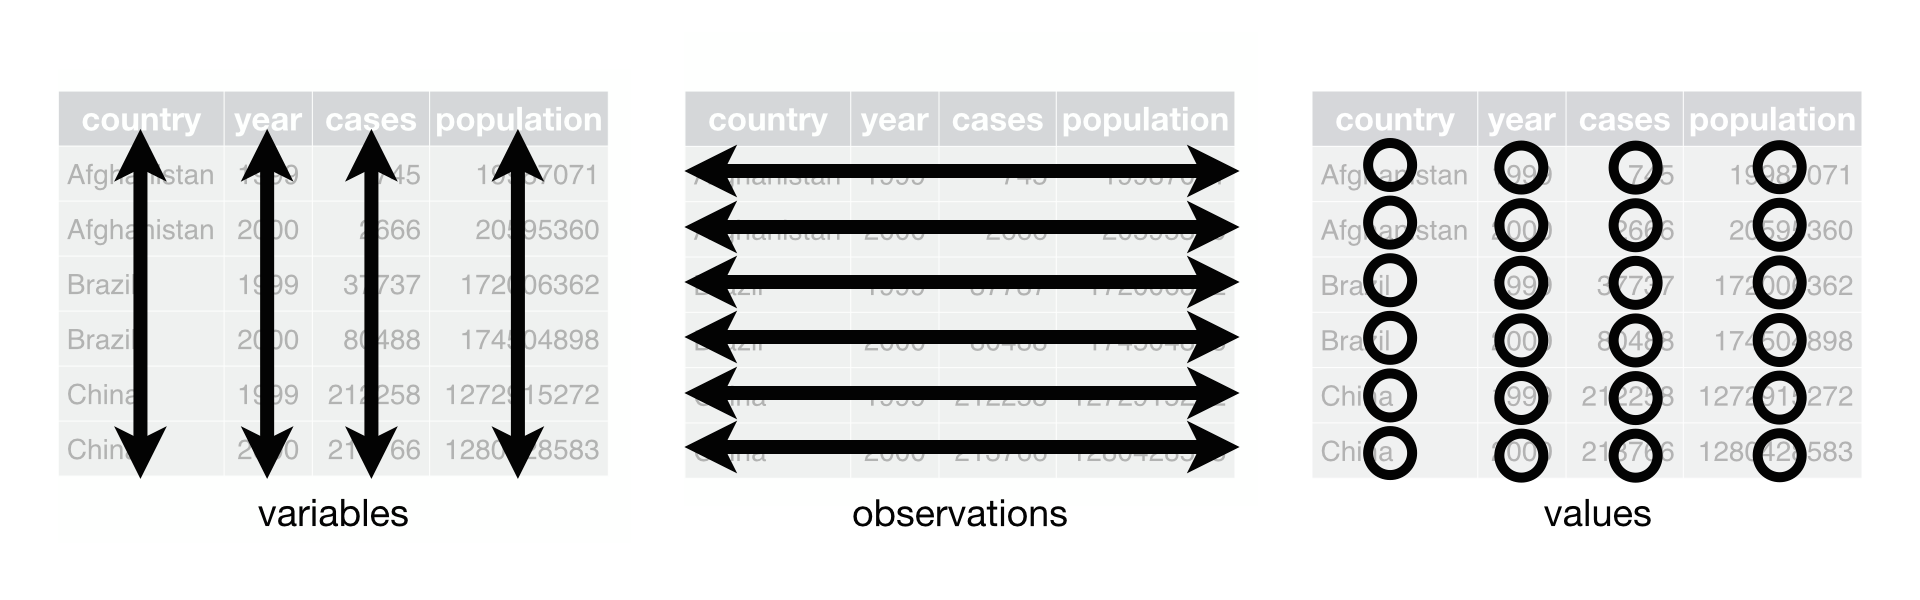
\includegraphics[width=0.75\linewidth,height=\textheight,keepaspectratio]{img/tidy-1.png}

}

\caption{\label{fig-tidy1}Tidy-Data-Sinnbild (Wickham, 2023)}

\end{figure}%

Tabelle~\ref{tbl-daten} ist ein Beispiel für Tidy-Data.
Abbildung~\ref{fig-tidy1} zeigt ein Sinnbild für Tidy-Data (Wickham \&
Grolemund, 2018). Für eine statistische Analyse ist es oft sinnvoll,
dass die Daten im Tidy-Format vorliegen. Der Vorteil des Tidy-Formats
ist es, dass man weiß, wie die Daten aufgebaut sind. Außerdem können
Statistikprogramme oft mit dieser Form am besten umgehen, s.
Abbildung~\ref{fig-tidy3}.

\begin{figure}

\centering{

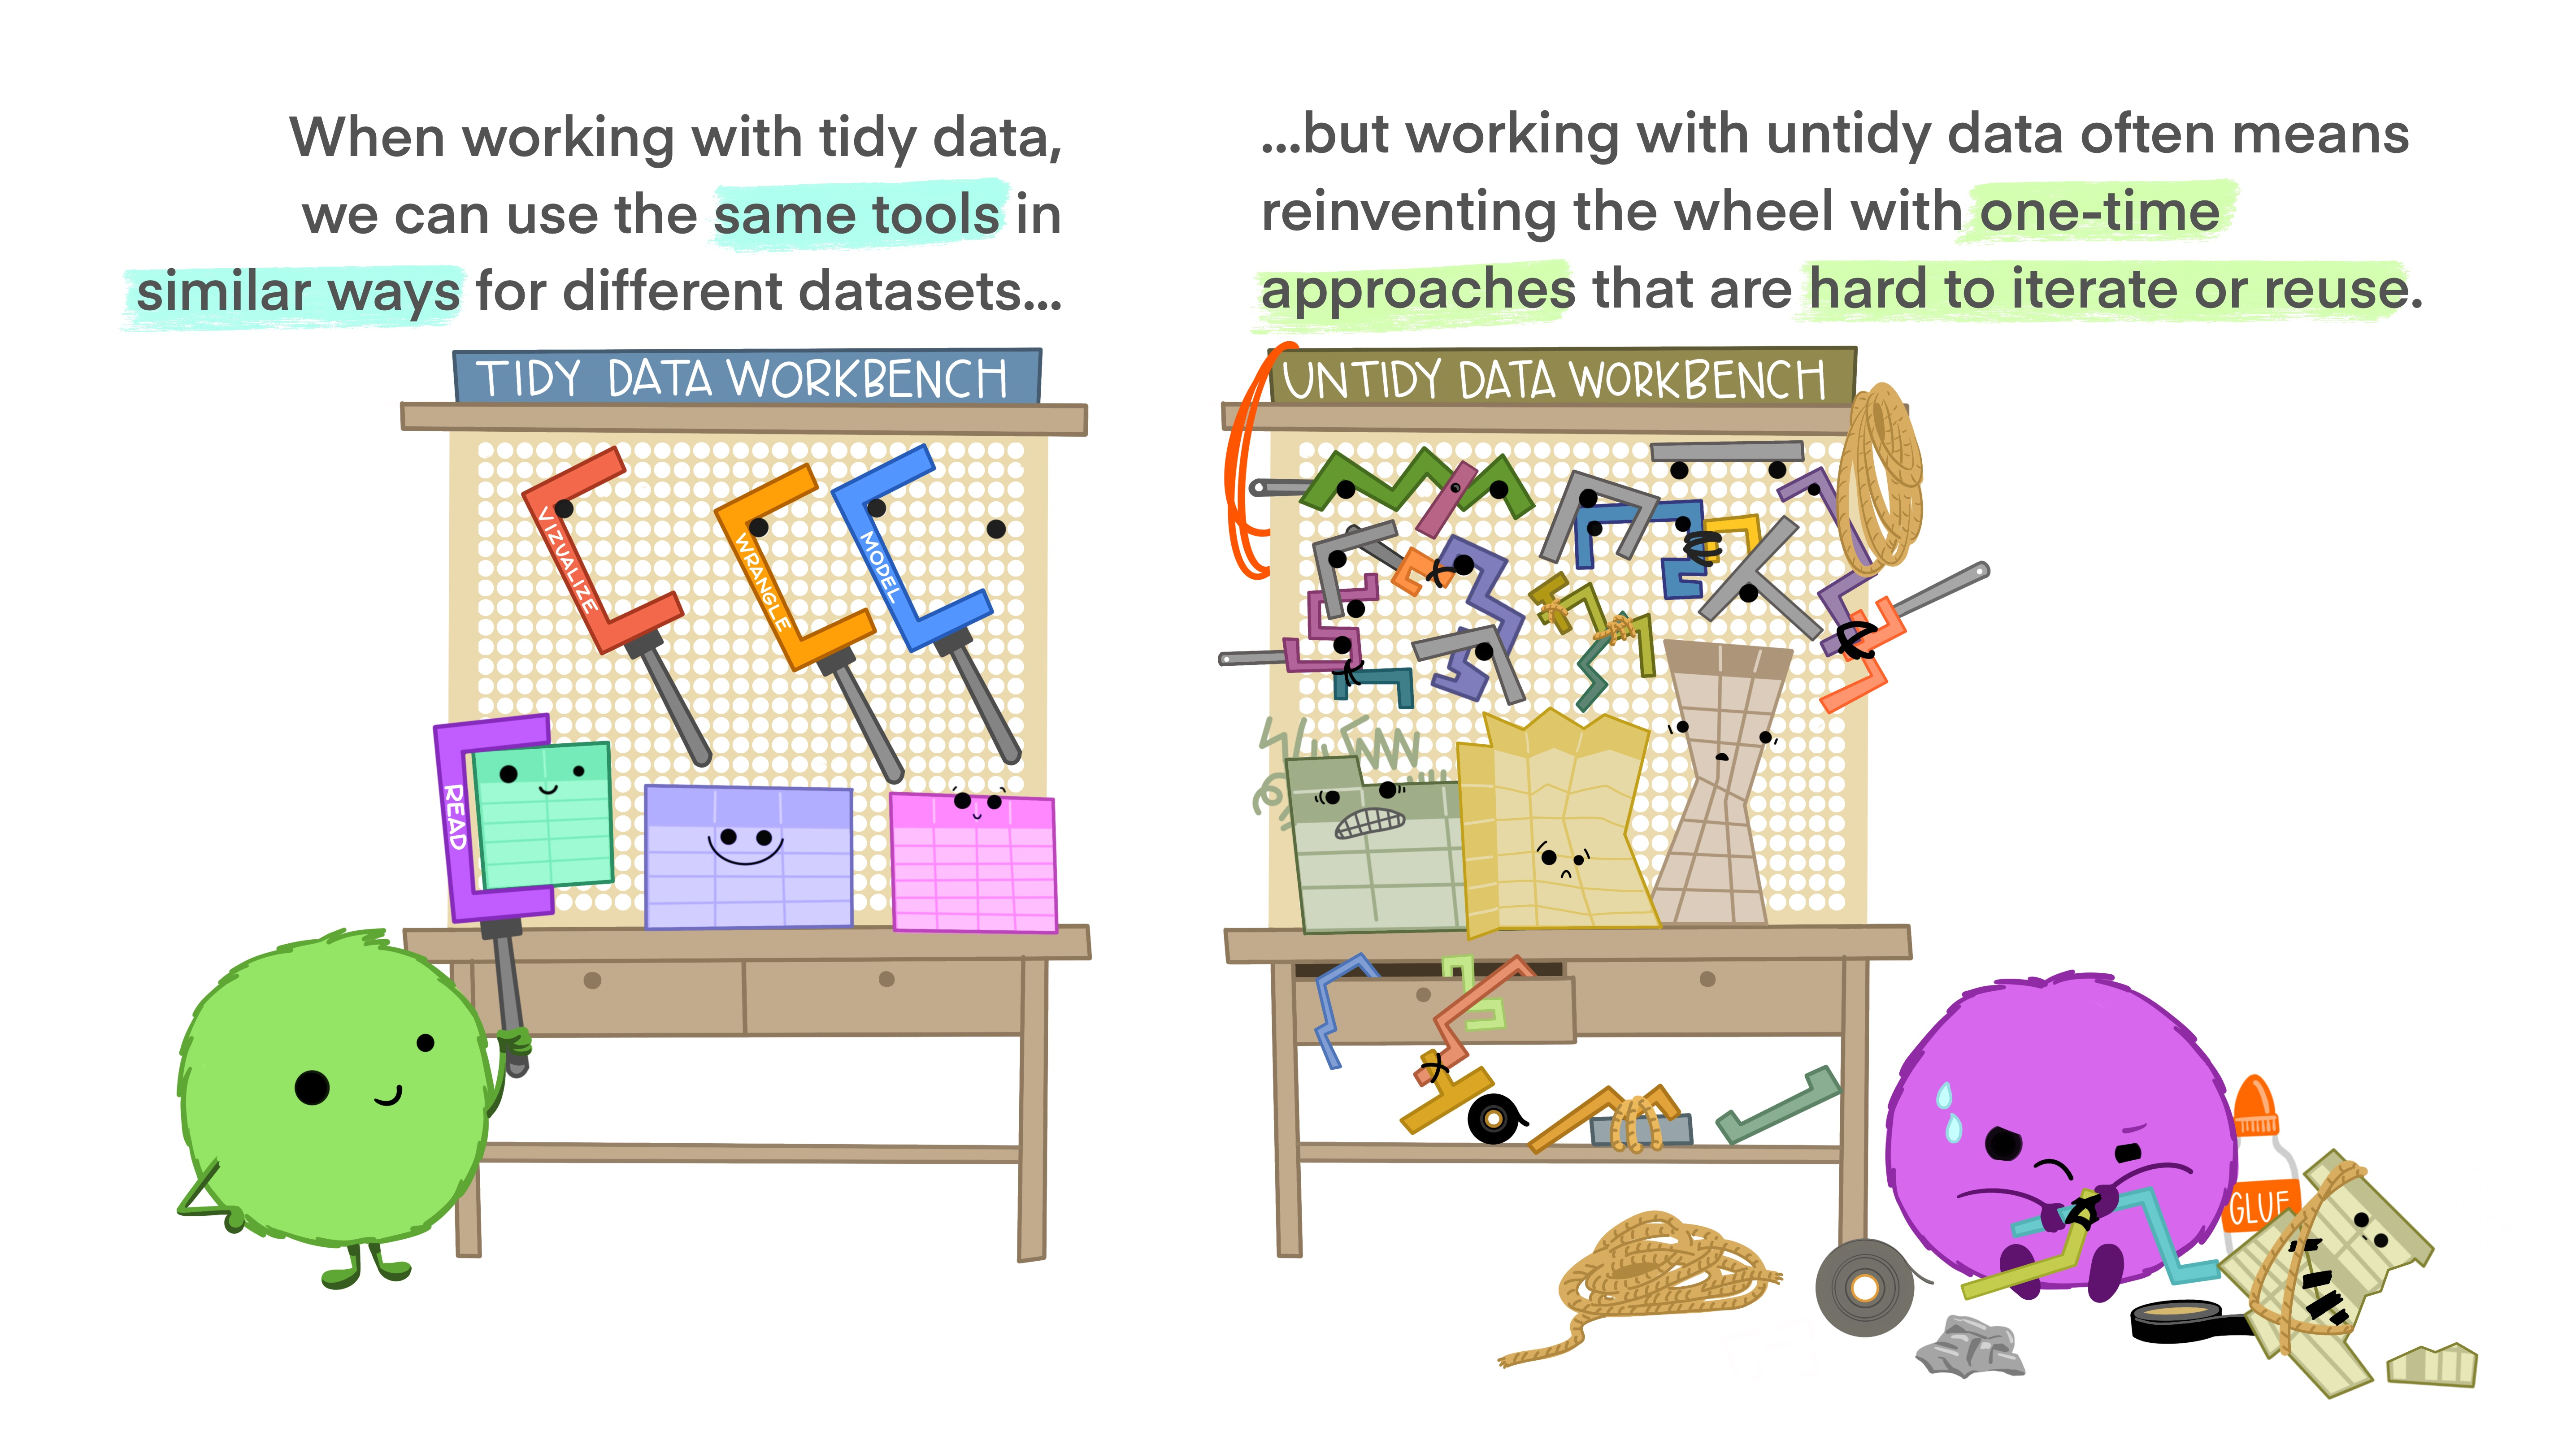
\includegraphics[width=0.75\linewidth,height=\textheight,keepaspectratio]{img/tidydata_3.jpg}

}

\caption{\label{fig-tidy3}Immer schön Ordnung halten\ldots{} (Horst,
2023)}

\end{figure}%

\begin{example}[]\protect\hypertarget{exm-widelong}{}\label{exm-widelong}

Ihre Firma produziert zwei Produkte: Hämmer und Nägel. Im Folgenden sind
zwei Tabellen dargestellt, die die gleichen Informationen darstellen:
den Umsatz Ihrer Firma für zwei Jahre. Einmal ist dazu eine
Nicht-Tidy-Tabelle (Tabelle~\ref{tbl-untidy1}; Breitformat) und einmal
eine Tidy-Tabelle (Tabelle~\ref{tbl-tidy1}; Langformat) verwendet.
\(\square\)

\end{example}

\begin{longtable}[]{@{}lrrr@{}}

\caption{\label{tbl-untidy1}Beispiel für eine NICHT-Tidy-Tabelle
(Breitformat)}

\tabularnewline

\toprule\noalign{}
Produkt & Umsatz\_2021 & Umsatz\_2022 & Umsatz\_2023 \\
\midrule\noalign{}
\endhead
\bottomrule\noalign{}
\endlastfoot
Hämmer & 10 & 11 & 12 \\
Nägel & 15 & 10 & 5 \\

\end{longtable}

\begin{longtable}[]{@{}llr@{}}

\caption{\label{tbl-tidy1}Beispiel für eine Tidy-Tabelle (Langformat)}

\tabularnewline

\toprule\noalign{}
Produkt & Jahr & Umsatz \\
\midrule\noalign{}
\endhead
\bottomrule\noalign{}
\endlastfoot
Hämmer & 2021 & 10 \\
Hämmer & 2022 & 11 \\
Hämmer & 2023 & 12 \\
Nägel & 2021 & 15 \\
Nägel & 2022 & 10 \\
Nägel & 2023 & 5 \\

\end{longtable}

\begin{exercise}[]\protect\hypertarget{exr-widelong}{}\label{exr-widelong}

Suchen Sie ein Beispiel für eine Konfiguration einer Tabelle im Lang-
vs.~Breitformat. \(\square\)

\end{exercise}

\begin{quote}
{\emoji{student}} Wozu braucht man Tidy Data?
\end{quote}

\begin{quote}
{\emoji{woman-teacher}} In vielen Software-Programmen der Datenanalyse
weißt man z.B. der X- oder Y-Variable eine Spalte einer Tabelle zu.
Möchte man etwa die Veränderung des Umsatzes im Verlauf der Jahre
visualisieren oder analysieren, so braucht es die Spalten
\enquote*{Jahr} und \enquote*{Umsatz}, also ein Tidy-Format,
Tabelle~\ref{tbl-untidy1} bzw. Tabelle~\ref{tbl-tidy1}.
\end{quote}

Abbildung~\ref{fig-tidy} stellt auf Basis einer \enquote{Tidy-Tabelle}
(Tabelle~\ref{tbl-tidy1}) ein Diagramm dar. Ohne Tidy-Daten wäre dieses
Diagramm nicht (so einfach) zu erstellen gewesen.

\begin{figure}

\centering{

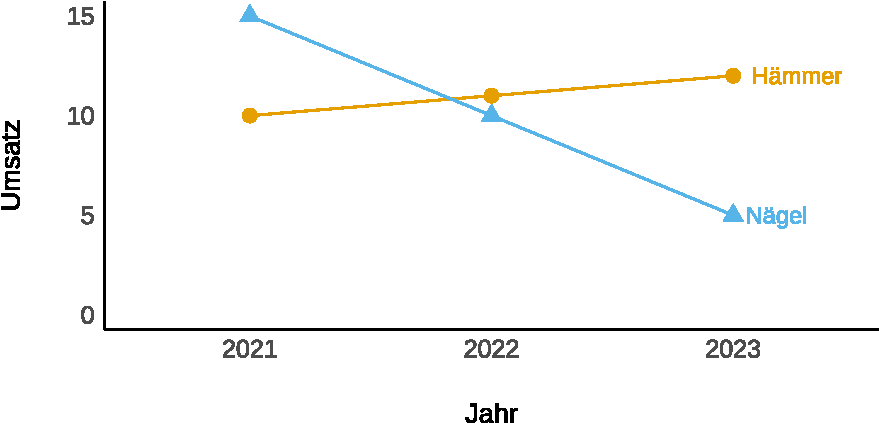
\includegraphics[width=0.75\linewidth,height=\textheight,keepaspectratio]{010-rahmen_files/figure-pdf/fig-tidy-1.pdf}

}

\caption{\label{fig-tidy}Beispiel für eine Visualisierung auf Basis
einer Tidy-Tabelle, vgl. Tabelle~\ref{tbl-tidy1}}

\end{figure}%

\subsection{Je mehr, desto besser (?)}\label{je-mehr-desto-besser}

Was Daten betrifft, könnte man behaupten: \enquote{Viel hilft viel} oder
\enquote{Je mehr, desto besser}. Natürlich unter sonst gleichen
Umständen.\footnote{Ceteris paribus, auf Latein, hört sich gleich viel
  schlauer an.} Viel Datenmüll ist natürlich nicht besser als ein paar
knappe, wasserdichte Fakten!

\begin{example}[]\protect\hypertarget{exm-samplesize}{}\label{exm-samplesize}

Um Ihre eigene Lehraktivität zu organisieren, wollen Sie sich ein Bild
machen, wie viel Ihre Nebensitzerinner und Nebensitzer im Hörsaal so
lernen. Sie blicken nach links und fragen \enquote{wie viel lernst du
so?}. Sie blicken nach recht und wiederholen die Frage gerichtet an den
Kommilitonen, der rechts neben Ihnen sitzt. Dann addieren Sie die zwei
Zahlen (unter der Annahme, dass Sie zwei Zahlen bekommen haben), und
teilen durch zwei, um den Mittelwert zu erhalten. \(\square\)

\end{example}

Ein kritischer Geist könnte anmerken, dass Sie besser die Untersuchung
nicht gemacht hätten (auch wenn Sie, vielleicht ohne zu wollen, eine
statistische Untersuchung angestellt haben). Denn bei so wenig befragten
Personen ist die Ungenauigkeit Ihrer Schätzung der typischen Lernzeit
bei Studierenden einfach zu hoch.

Abbildung~\ref{fig-sample-estimate} veranschaulicht, dass man einen
Mittelwert genauer schätzen kann, wenn man auf eine größere Stichprobe
zurückgreift. Das Teilbild links zeigt den Mittelwert einer Stichprobe
mit \(n=20\) Beobachtungen. Das Teilbild rechts zeigt den Mittelwert
einer Stichprobe mit \(n=200\) Beobachtungen (jeweils aus der gleichen
Grundgesamtheit). Wie man sieht, ist im linken Teilbild die Streuung
(Variation) höher als im rechten Teilbild:

\begin{figure}

\centering{

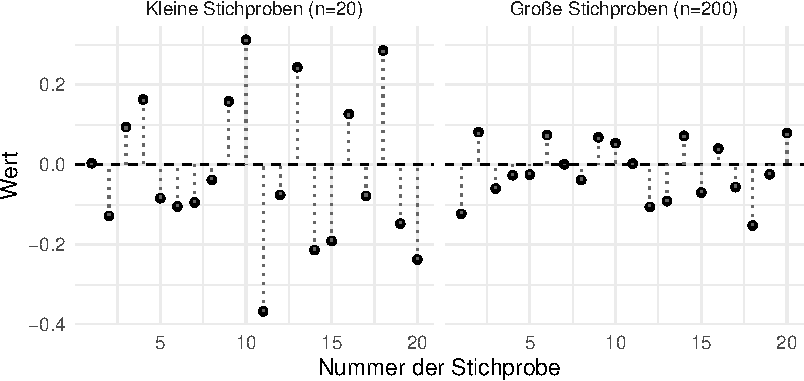
\includegraphics[width=1\linewidth,height=\textheight,keepaspectratio]{010-rahmen_files/figure-pdf/fig-sample-estimate-1.pdf}

}

\caption{\label{fig-sample-estimate}Schätzgenauigkeit als Funktion der
Stichprobengröße. Jeder Punkt stellt eine Stichprobe dar, entweder mit
\(n=20\) (links) oder mit \(n=200\) (rechts). Kleine Stichproben (links)
haben im Schnitt eine größere Abweichung vom wahren Mittelwert als
größere Stichproben (rechts).}

\end{figure}%

\begin{tcolorbox}[enhanced jigsaw, leftrule=.75mm, breakable, left=2mm, colback=white, colframe=quarto-callout-important-color-frame, opacitybacktitle=0.6, coltitle=black, colbacktitle=quarto-callout-important-color!10!white, arc=.35mm, bottomtitle=1mm, toprule=.15mm, rightrule=.15mm, toptitle=1mm, titlerule=0mm, title=\textcolor{quarto-callout-important-color}{\faExclamation}\hspace{0.5em}{Wichtig}, bottomrule=.15mm, opacityback=0]

Mehr Daten = genauere Ergebnisse (unter sonst gleichen Umständen)
\(\square\)

\end{tcolorbox}

\begin{exercise}[Live-Experiment zum Effekt der
Stichprobengröße]\protect\hypertarget{exr-kleine-grosse-stipro}{}\label{exr-kleine-grosse-stipro}

In diesem Live-Experiment untersuchen wir den Effekt der
\emph{Stichprobengröße} auf die Streuung des Mittelwerts in der
\emph{Stichprobe.} Streuen die Ergebnisse mehr in kleinen Stichproben
als in großen? Probieren wir es aus!

In diesem Experiment werfen Sie (in kleinen Gruppen) eine Münze (auf
faire Art und Weise) und notieren das Ergebnis (Kopf oder Zahl). Uns
interessiert dabei die Frage, ob die Ergebnisse bei kleinen Stichproben
(\(n=5\) Münzwürfe) anders streuen als in großen Stichproben (\(n=20\)
Münzwürfe).

\begin{figure}

\begin{minipage}{0.80\linewidth}
Sie brauchen nur experimentierfreudige Partner (Kleingruppen mit 2-4
Personen), eine faire Münze und dann kann's los gehen!
\href{https://docs.google.com/forms/d/e/1FAIpQLSeAwqNyZtyQwttq5JrQdQ2AO7w5vzcVDXjiejKnyFNxiWtEag/viewform?usp=sf_link}{Scannen
Sie den QR-Code, um mit dem Experiment zu starten}.\end{minipage}%
%
\begin{minipage}{0.20\linewidth}

\begin{center}

\includegraphics[width=0.75\linewidth,height=\textheight,keepaspectratio]{010-rahmen_files/figure-pdf/unnamed-chunk-17-1.pdf}
\end{center}

\end{minipage}%

\end{figure}%

Die Daten aller Versuche können Sie
\href{https://docs.google.com/spreadsheets/d/11mKFFpr-Y1CMPpq4dGA-JA_Z9jRkPbXolo54Y0G_2gE/edit?usp=sharing}{hier}
einsehen.\footnote{\url{https://tinyurl.com/3w8ke2n2}} \(\square\)

\end{exercise}

\begin{example}[Dorfschulen machen die schlauesten
Schüler?!]\protect\hypertarget{exm-schule-samplesize}{}\label{exm-schule-samplesize}

In einer Pressemitteilung sei zu lesen, dass die besten Schüler in den
Dorfschulen zu finden seien. (Das ist eine fiktive Geschichte.) Mit
etwas Recherche finden Sie heraus, dass diese Aussage auf belastbaren
Daten beruht: Tatsächlich sind die Notendurchschnitte auf den kleinen
Dorfschulen deutlich besser als in den großen Schulen in der Stadt. Also
stimmt die Behauptung der Pressemitteilung? Die gute Landluft lässt das
Hirn wachsen? Sie recherchieren noch etwas weiter in den Daten. Dann
fällt Ihnen auf: Die \emph{schlechtesten} Schüler kommen auch aus den
Dorfschulen! Eine statistische Erklärung bietet sich an: In den
Dorfschulen gibt es nur wenig Kinder und vergleichsweise‚ kleine Klassen
-- die Stichproben sind also klein. Bei kleinen Stichproben gibt es viel
Variation um den Mittelwert herum, s.
Abbildung~\ref{fig-sample-estimate}, und zwar nach oben (guter
Notenschnitt) und nach unten (schlechter Notenschnitt). \(\square\)

\end{example}

\section{Arten von Variablen}\label{sec-arten-variablen}

\subsection{Nach Position in der
Forschungsfrage}\label{nach-position-in-der-forschungsfrage}

Angenommen, Ihre Forschungsfrage lautet:

\begin{quote}
Hat Lernen einen Einfluss auf den Prüfungserfolg?
\end{quote}

In dem Fall gilt:

\emph{Lernen} ist die Input-Variable, X-Variable, Ursache, unabhängig
Variable (UV). \emph{Prüfungserfolg} ist die Output-Variable,
Y-Variable, Wirkung, abhängige Variable (AV)

Abbildung~\ref{fig-ueberblick-fragen} stellt diese beiden
\enquote{Positionen} einer Variable dar. Die erste Position ist vor dem
Pfeil (X). Die zweite Position ist nach dem Pfeil (Y).

\begin{figure}

\centering{

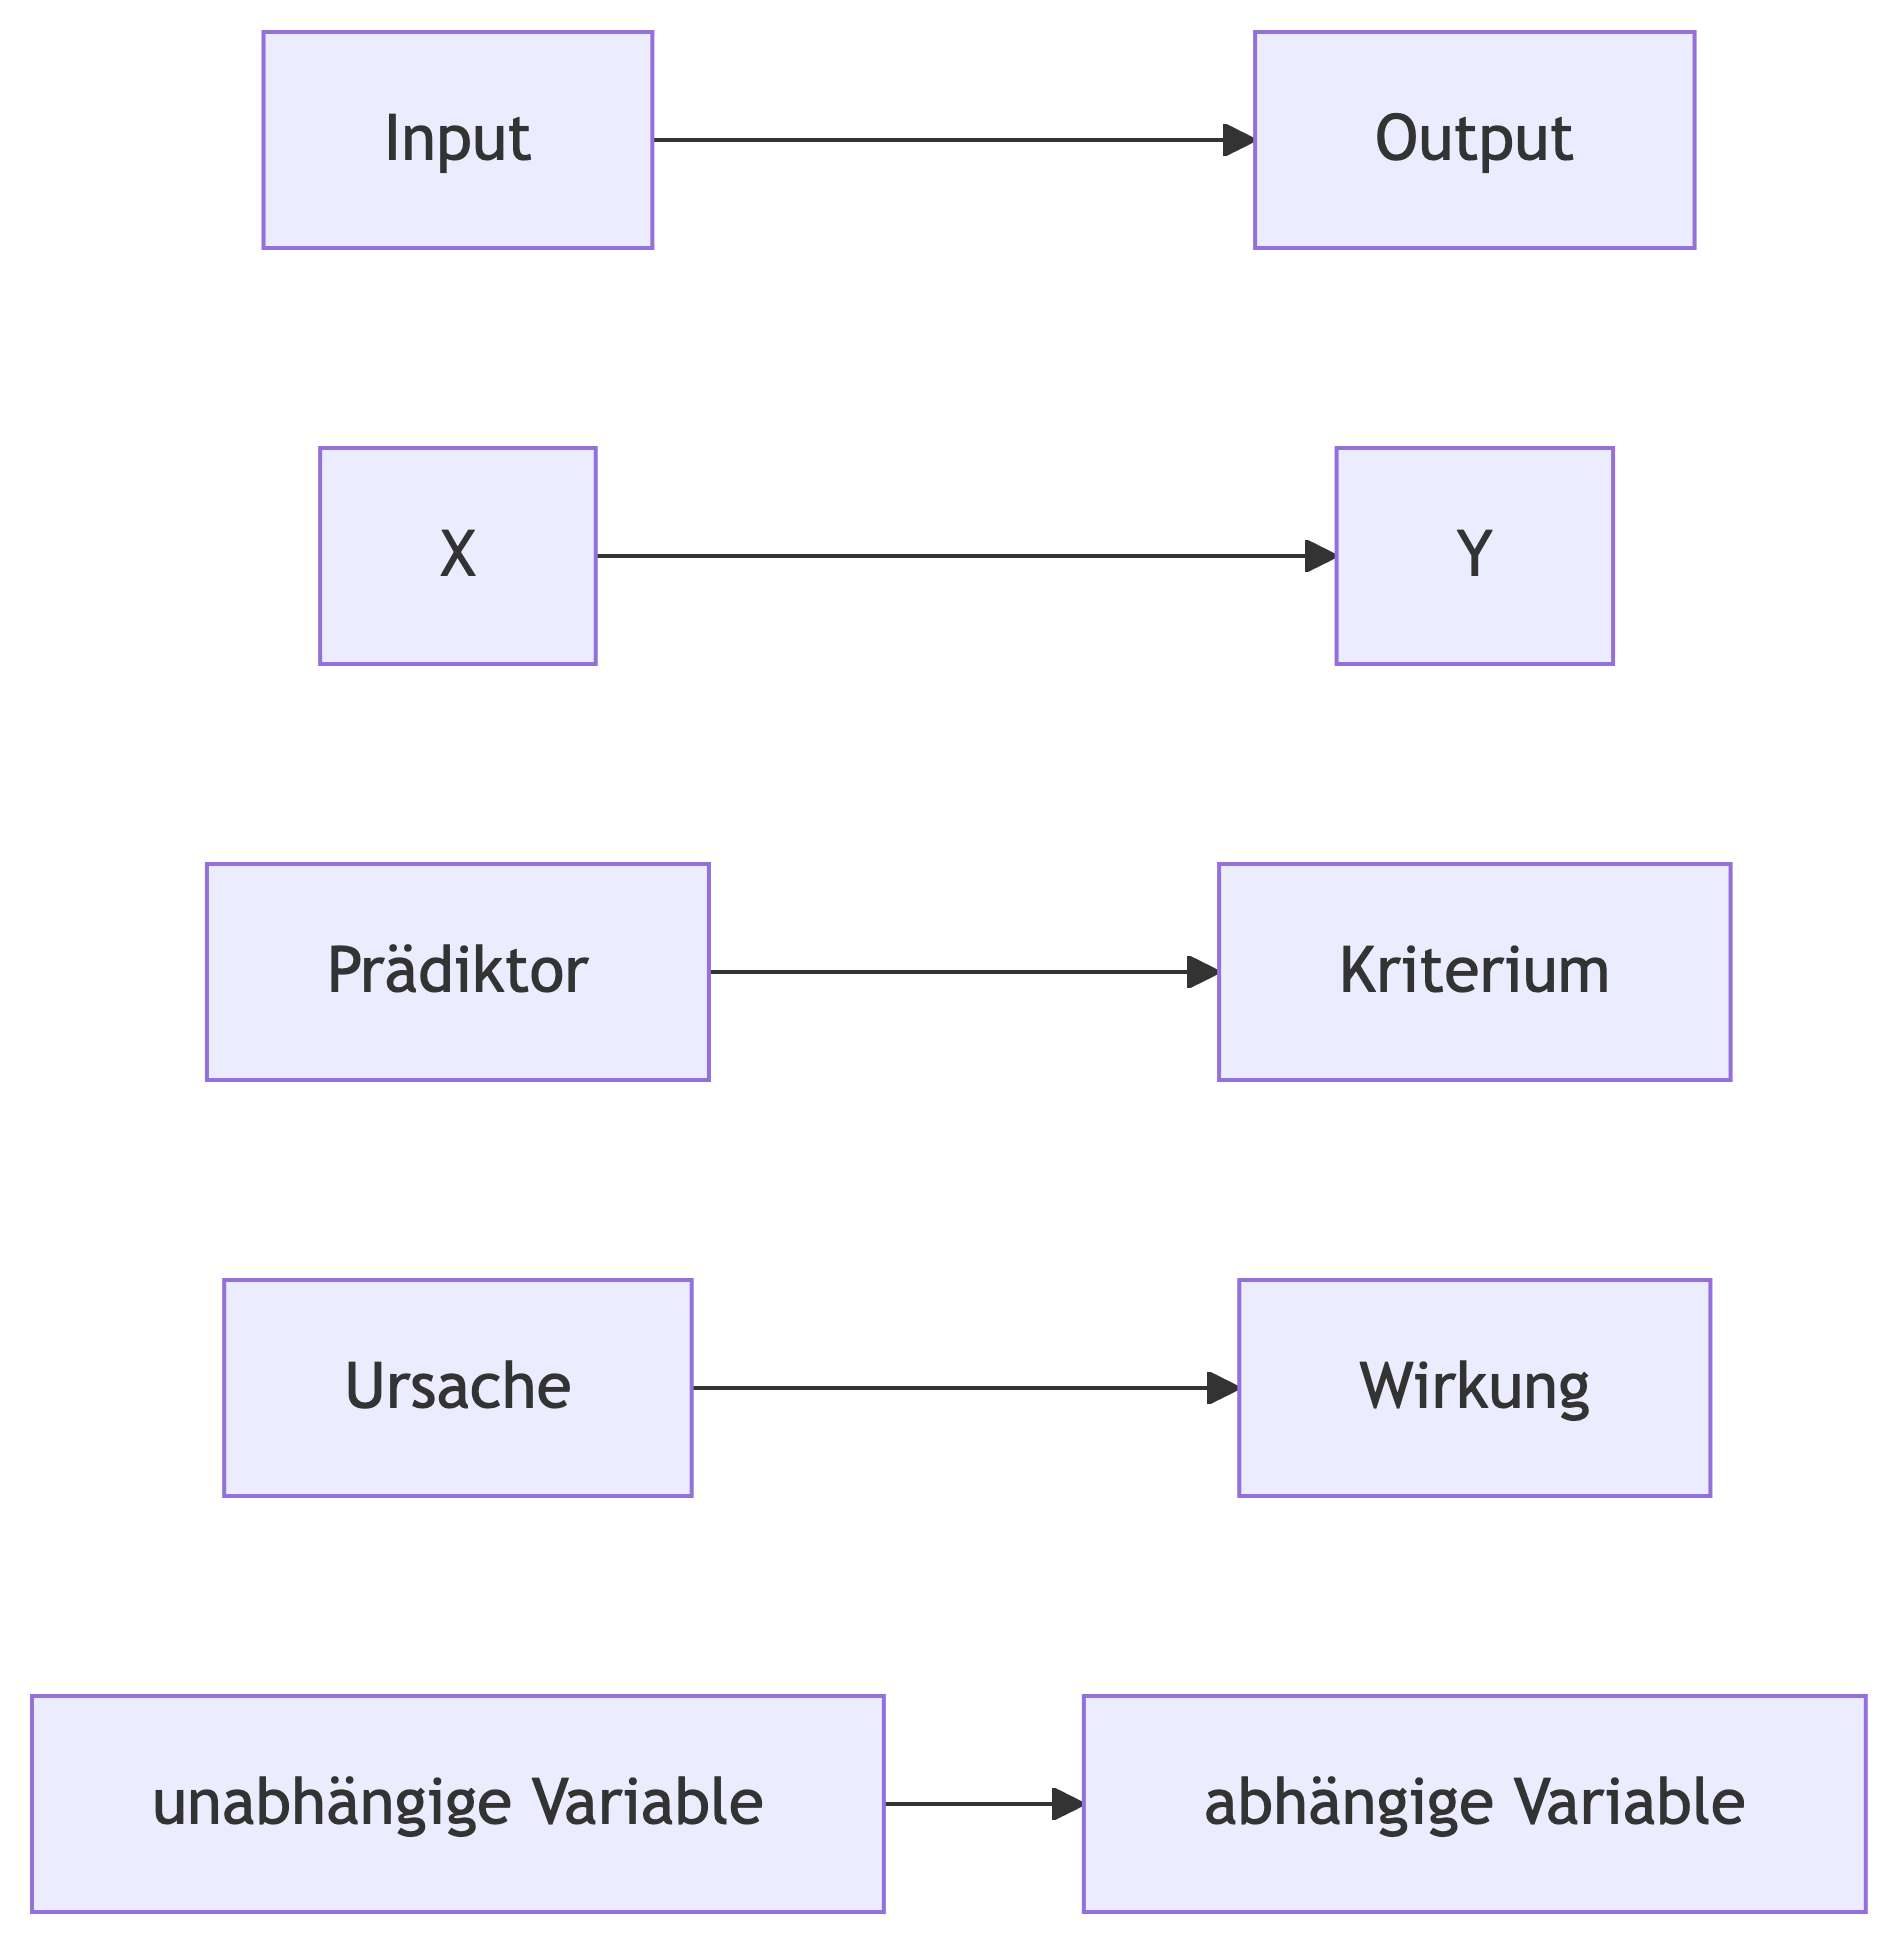
\includegraphics[width=1.63in,height=0.5in]{010-rahmen_files/figure-latex/mermaid-figure-3.png}

}

\caption{\label{fig-ueberblick-fragen}X und Y als synonyme Bezeichnungen
für Input- und Output-Variablen einer Forschungsfrage}

\end{figure}%

\begin{exercise}[]\protect\hypertarget{exr-uvav}{}\label{exr-uvav}

Überlegen Sie sich eine Forschungsfrage, die eine UV und eine AV
enthält. Nennen Sie einer anderen Person diese Forschungsfrage und
fragen Sie, was die UV und die AV ist. Bei richtiger Antwort belohnen
Sie großzügig. \(\square\)

\end{exercise}

\subsection{Nach dem Skalenniveau}\label{nach-dem-skalenniveau}

\begin{definition}[Skalenniveau]\protect\hypertarget{def-skalenniveau}{}\label{def-skalenniveau}

Der Begriff \emph{Skalenniveau} wird verwendet, um die Art und Menge der
Information, die in Variablen enthalten ist, zu benennen. Diese
Klassifikation basiert auf den Eigenschaften der Daten und den
mathematischen Operationen, die sinnvoll auf diese Daten angewendet
werden können. \(\square\)

\end{definition}

Abbildung~\ref{fig-skalenniveau} gibt einen Überblick über typisch
verwendete Skalenniveaus.

\begin{figure}

\centering{

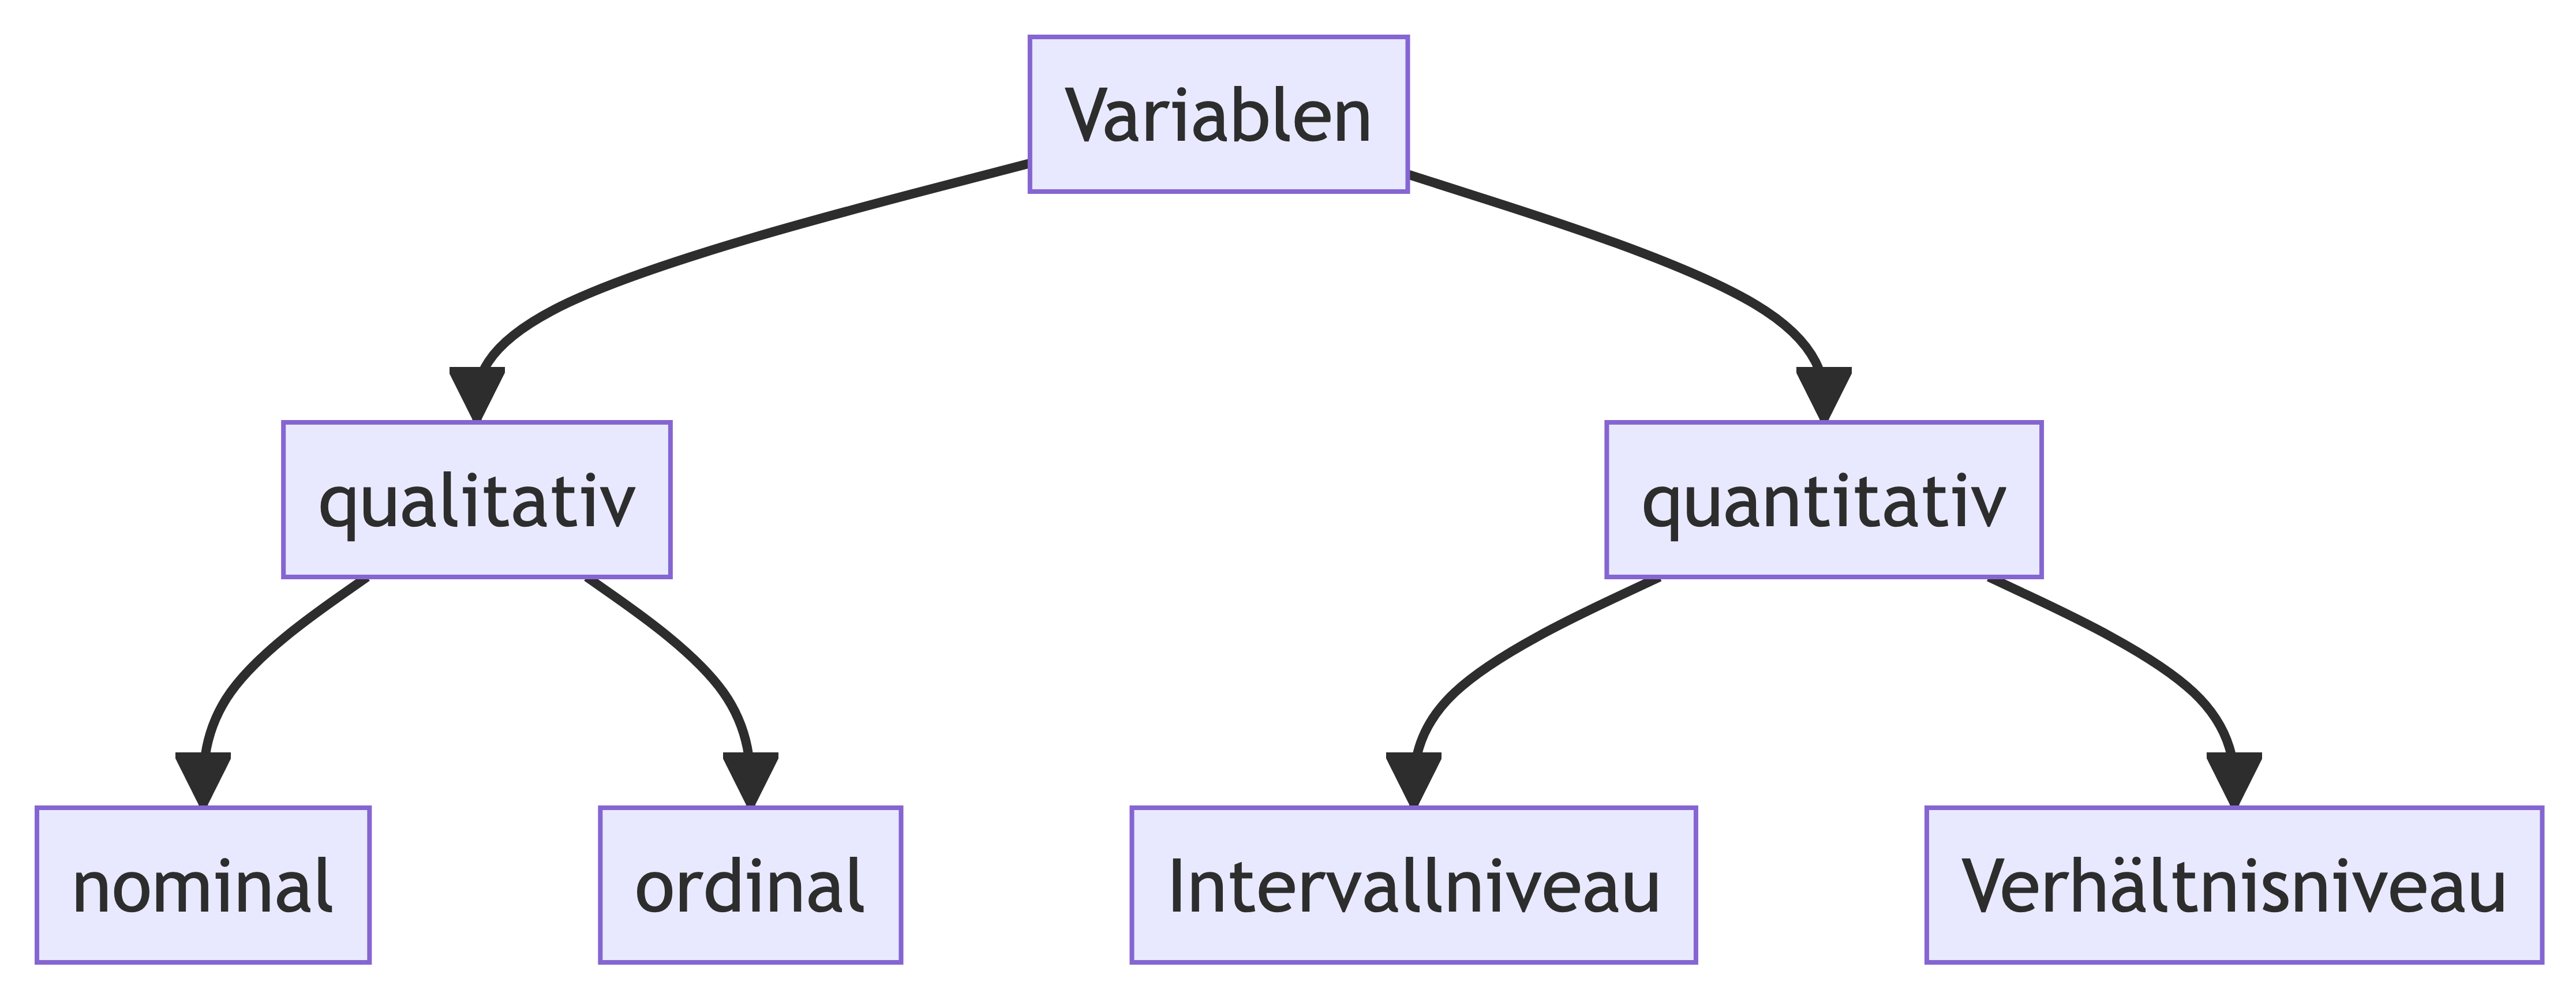
\includegraphics[width=4in,height=1.51in]{010-rahmen_files/figure-latex/mermaid-figure-2.png}

}

\caption{\label{fig-skalenniveau}Skalenniveaus}

\end{figure}%

\subsection{Beispiele für
Skalenniveaus}\label{beispiele-fuxfcr-skalenniveaus}

Beispiele zu den Skalenniveaus sind in Tabelle~\ref{tbl-skalen-bsps}
aufgeführt. \(\square\)

\begin{longtable}[]{@{}ll@{}}

\caption{\label{tbl-skalen-bsps}Beispiele für Skalenniveaus}

\tabularnewline

\toprule\noalign{}
Variable & Skalenniveau \\
\midrule\noalign{}
\endhead
\bottomrule\noalign{}
\endlastfoot
Haarfarbe & Nominalskala \\
Augenfarbe & Nominalskala \\
Geschlecht & Nominalskala \\
Automarke & Nominalskala \\
Partei & Nominalskala \\
Lieblingsessen & Ordinalskala \\
Medaillen beim 100-Meter-Lauf & Ordinalskala \\
Uniranking & Ordinalskala \\
IQ & Intervallskala \\
Extraversion & Intervallskala \\
Temperatur in Celsius & Intervallskala \\
Temperatur in Fahrenheit & Intervallskala \\
Temperatur in Kelvin & Verhältnisskala \\
Körpergröße & Verhältnisskala \\
Geschwindigkeit & Verhältnisskala \\
Länge & Verhältnisskala \\

\end{longtable}

Jenachdem, über welches Skalenniveau eine Variable verfügt, sind
verschiedenen Rechenoperationen erlaubt, s.
{Tabelle~\ref{tbl-skalenniveaus-pdf}}.

\begin{longtable}[]{@{}
  >{\raggedright\arraybackslash}p{(\linewidth - 10\tabcolsep) * \real{0.2073}}
  >{\raggedright\arraybackslash}p{(\linewidth - 10\tabcolsep) * \real{0.1585}}
  >{\raggedright\arraybackslash}p{(\linewidth - 10\tabcolsep) * \real{0.1585}}
  >{\raggedright\arraybackslash}p{(\linewidth - 10\tabcolsep) * \real{0.1585}}
  >{\raggedright\arraybackslash}p{(\linewidth - 10\tabcolsep) * \real{0.1585}}
  >{\raggedright\arraybackslash}p{(\linewidth - 10\tabcolsep) * \real{0.1585}}@{}}

\caption{\label{tbl-skalenniveaus-pdf}Erlaubte Rechenoperationen nach
Skalenniveau (ja, erlaubt: \(\checkmark\); nein, nicht erlaubt:
\(\times\))}

\tabularnewline

\toprule\noalign{}
\begin{minipage}[b]{\linewidth}\raggedright
Skalenniveau
\end{minipage} & \begin{minipage}[b]{\linewidth}\raggedright
Quantitativ
\end{minipage} & \begin{minipage}[b]{\linewidth}\raggedright
≠
\end{minipage} & \begin{minipage}[b]{\linewidth}\raggedright
\(\preceq\)
\end{minipage} & \begin{minipage}[b]{\linewidth}\raggedright
+
\end{minipage} & \begin{minipage}[b]{\linewidth}\raggedright
×
\end{minipage} \\
\midrule\noalign{}
\endhead
\bottomrule\noalign{}
\endlastfoot
Nominalniveau & \(\times\) & \(\checkmark\) & \(\times\) & \(\times\) &
\(\times\) \\
Ordinalniveau & \(\times\) & \(\checkmark\) & \(\checkmark\) &
\(\times\) & \(\times\) \\
Intervallniveau & \(\checkmark\) & \(\checkmark\) & \(\checkmark\) &
\(\checkmark\) & \(\times\) \\
Verhältnisniveau & \(\checkmark\) & \(\checkmark\) & \(\checkmark\) &
\(\checkmark\) & \(\checkmark\) \\

\end{longtable}

Was soll das bedeuten, \enquote{Rechenoperationen}? Schauen wir uns für
jedes Skalenniveau ein \enquote{Rechenbeispiel} an.

\emph{Nominalskala}: Die Variable \emph{Geschlecht} ist nominalskaliert.
Das bedeutet, dass ihre Ausprägungen \emph{Frau} und \emph{Mann} z.B.
nicht (sinnvoll) addiert oder sonstwie \enquote{verrechnet} werden
können. Man könnte, z.B. um das Eintippen zu erleichtern, Frauen mit
\texttt{1} kodieren und Männer mit \texttt{2}. Damit darf man aber nicht
rechnen! Nicht addieren, nicht multiplizieren, etc. Es macht keinen Sinn
zu sagen: \enquote{Ich habe eine Frau und einen Mann in meiner Tabelle,
das ist im Schnitt ein diverses Geschlecht, weil der Mittelwert von 1
und 2 ist 1,5!} Die \emph{einzige} \enquote{Rechenoperation}, die man
auf der Nominalskala machen darf, ist die Prüfung auf \emph{Gleichheit}:
Mann kann feststellen, ob ein Objekt gleich zu einem anderen ist oder
unterschiedlich. Also ob zwei Personen das gleiche Geschlecht haben oder
von unterschiedlichem Geschlecht sind. Anders ausgedrückt:

\begin{itemize}
\tightlist
\item
  FRAU \(\ne\) MANN
\item
  FRAU \(=\) FRAU
\item
  MANN \(=\) MANN
\end{itemize}

\emph{Ordinalskala}: Diese Skala stellt einer Rangordnung dar. Eine
Rangordnung ist etwa die geordnete Abfolge Ihres Leibgerichte (1. Pizza,
2. Spagetthi, 3. Schnitzel). Etwas \enquote{formaler} ausgedrückt, z.B.:

\begin{itemize}
\tightlist
\item
  \(\text{Pizza} \succ \text{Spagetthi} \succ \text{Schnitzel}\)
\end{itemize}

Das komische Zeichen \(\succ\) soll heißen: \enquote{Ist auf meiner
Liste von Leibgerichten weiter oben, mag ich lieber}. Man kann aber
\emph{nicht} sagen, \enquote{Ich mag aber Pizza um 42\% mehr als die
Spagetthi und die wieder um 73\% mehr als ein Schnitzel!}. Zumindest
kann man das nicht ohne weitere Informationen und Annahmen. Es gibt also
Dinge auf der Welt, die man (leicht in eine Rangordnung bringen kann,
aber die man nur schwer in der Größe der Unterschiede bemessen kann. Das
ist die Ordinalskala. Die Ordinalskale erlaubt also, Objekte zu ordnen
(hinsichtlich eines Merkmals). Die Abstände zwischen den Objekten können
dabei nicht quantifiziert werden.

\emph{Intervallskala}: Das ist vielleicht eine Überraschung für Sie:
Wenn es heute 10°C hat und morgen 5°C -- dann ist es heute \emph{nicht}
doppelt so warm wie morgen. Ja, 10 ist das Doppelte von 5. Aber
\emph{10° Celsius} ist \emph{nicht} doppelt so warm wie 20° Celsius.
Wenn Sie das verwundert: Das ist normal, so geht es vielen Leuten, wenn
sie das zum ersten Mal hören. Der Grund, dass es nicht erlaubt ist,
Verhältnisse (wie doppelt/halb so viel etc.) auf der Celsius-Skala zu
bilden, ist, dass der Nullpunkt der Skala, 0° C, kein echter,
physikalischer Nullpunkt ist. Bei 0° C liegt eben nicht Null
Wärmeenergie vor. Stattdessen wurde mit 0° C eine Wärmenergiemenge
gewählt, die für uns Menschen ganz praktisch, da augenfällig ist: der
Gefrierpunkt von Wasser. Was bei der Intervallskala erlaubt ist, ist das
Addieren (und Subtrahieren): heute 10°C, morgen 5°C, das ist ein
Unterschied von 5°C. Oder: Im Schnitt waren es 7,5°C, das ist genau in
der Mitte von 5 und 10°C. Abbildung~\ref{fig-intervall} versinnbildlicht
die Intervallskala.

\begin{figure}

\centering{

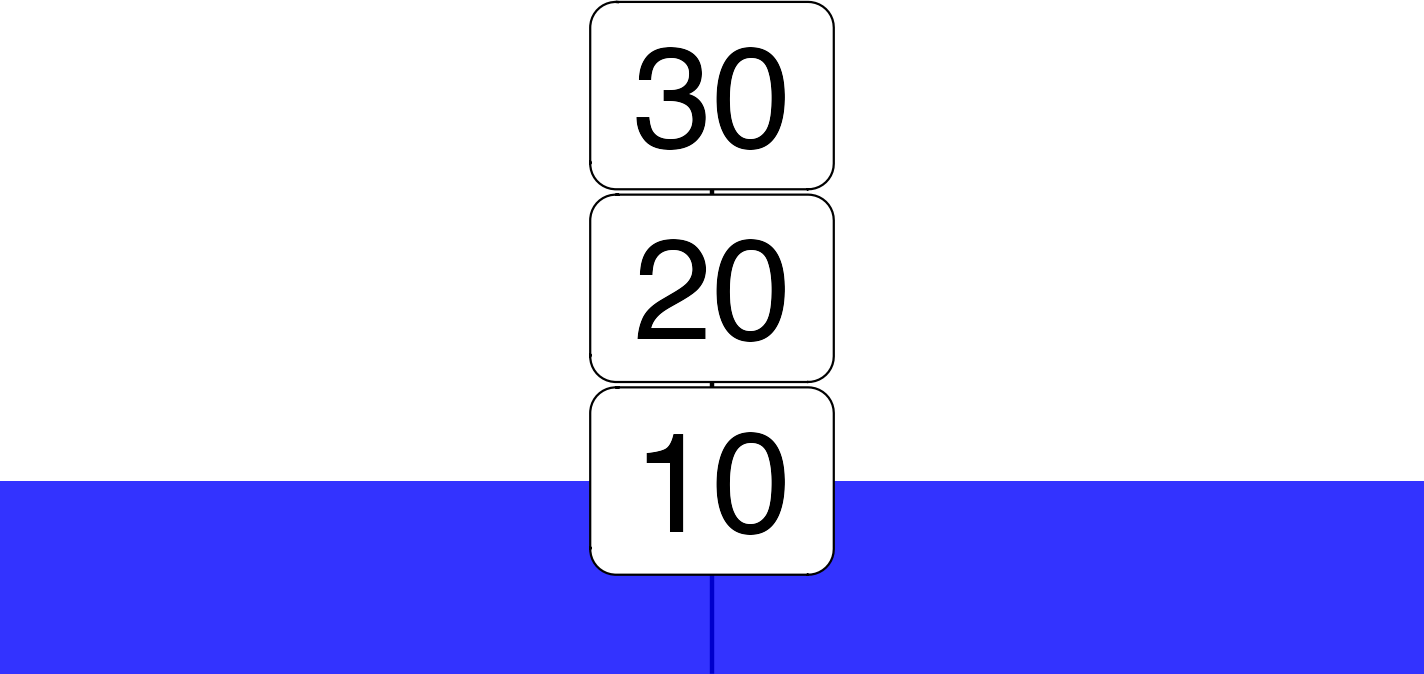
\includegraphics[width=1\linewidth,height=\textheight,keepaspectratio]{010-rahmen_files/figure-pdf/fig-intervall-1.png}

}

\caption{\label{fig-intervall}Ein Metermaß steckt im trüben Wasser. Auf
dem Metermaß können wir die aufgedruckten Zahlen ablesen. Aber wir
wissen nicht, ob der Metermaß auf dem Boden steht. Wir wissen demnach
nicht, ob der vom Metermaß angegebene Nullpunkt der wahre Nullpunkt
(Meeresboden) ist.}

\end{figure}%

\emph{Verhältnisskala}: Eine Verhältnisskala ist das, was man sich
gemeinhin unter einer metrische Variable vorstellt: Man kann
\enquote{normal} rechnen, alle Rechenoperationen sind erlaubt. Zuzüglich
zu denen, die auch in anderen, \enquote{niedrigeren} Skalenniveaus
erlaubt sind, ist das das Bilden von Verhältnissen -- Multiplizieren
(und damit auch Dividieren), s. Abbildung~\ref{fig-verhaeltnis}.

\begin{figure}

\centering{

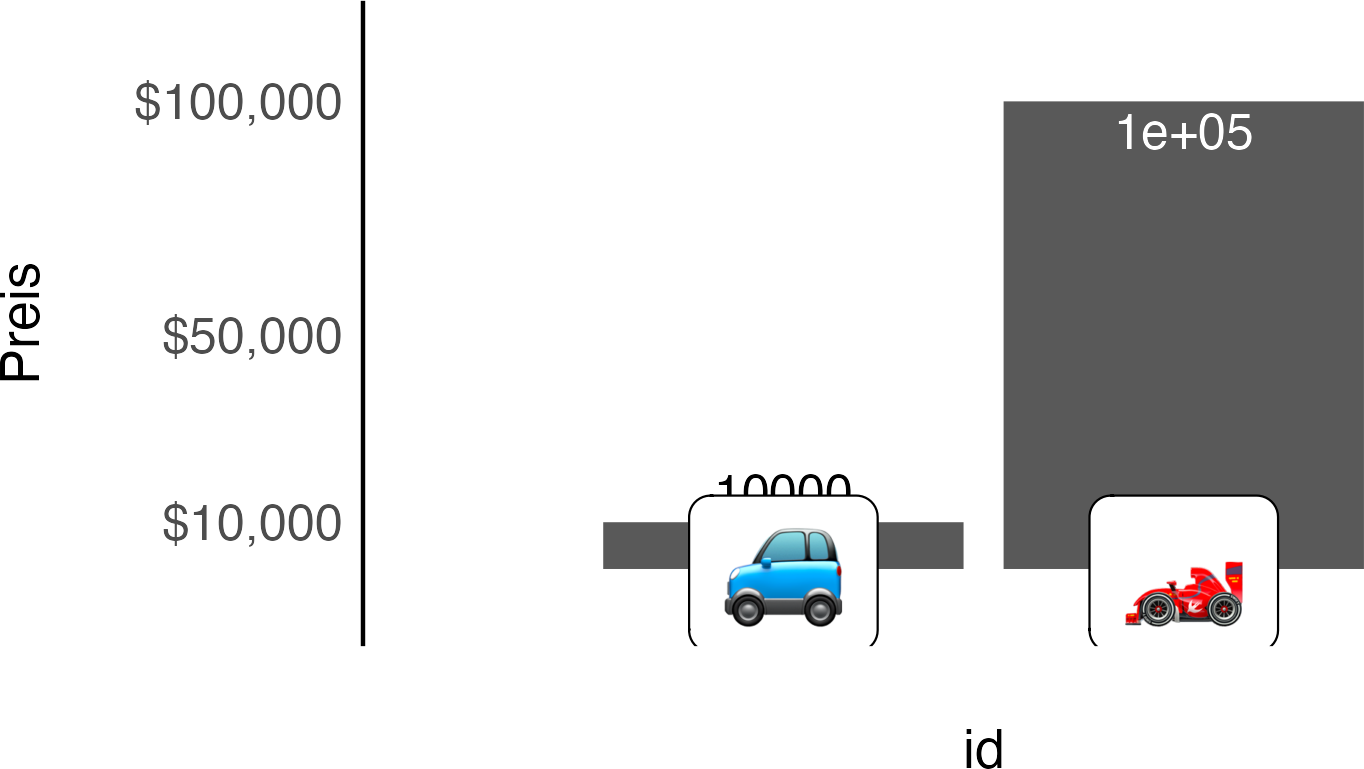
\includegraphics[width=1\linewidth,height=\textheight,keepaspectratio]{010-rahmen_files/figure-pdf/fig-verhaeltnis-1.png}

}

\caption{\label{fig-verhaeltnis}Puh! Der rote Flitzer ist 10 Mal so
teuer wie die blaue Möhre. Kohlen zusammenkratzen.}

\end{figure}%

\begin{figure}

\begin{minipage}{0.80\linewidth}
In \href{https://www.youtube.com/watch?v=_mN3kFe56ng}{diesem Video} gibt
es noch ausführlichere Erklärung zum Thema Skalenniveaus.\end{minipage}%
%
\begin{minipage}{0.20\linewidth}

\begin{center}

\includegraphics[width=0.75\linewidth,height=\textheight,keepaspectratio]{010-rahmen_files/figure-pdf/qr-youtube-skalenniveaus-1.pdf}
\end{center}

\end{minipage}%

\end{figure}%

Außerdem können quantitative Variablen wie folgt untergliedert werden:

\begin{itemize}
\tightlist
\item
  \emph{stetige} Variablen, das sind Variablen, bei denen man zwischen
  zwei Ausprägungen immer noch eine weitere quetschen kann. So gibt es
  einen Wert für die Köpergröße zwischen 1.60\,m und 1.61\,m. Und einen
  Wert zwischen 1.601\,m und 1.602\,m, etc.
\item
  \emph{diskrete} Variablen, das sind metrische Variablen, die nur
  bestimmte Ausprägungen haben, häufig sind das die natürlichen Zahlen:
  \(1,2,...\). Ein Beispiel wäre die Anzahl der Kinder in einer Familie.
\end{itemize}

Fragen nach Skalenniveaus gehören zu den Lieblingsprüfungsfragen in
diesem Themenbereich. Sie sind gut beraten, sich gerade mit dieser Frage
intensiver zu beschäftigen. Auch in thematisch angrenzenden Fächern wird
immer wieder die Frage nach dem Skalenniveau aufgeworfen. Das zeigt
natürlich auch die hohe Relevanz des Themas.

\begin{exercise}[]\protect\hypertarget{exr-skalenniveaus}{}\label{exr-skalenniveaus}

Überlegen Sie sich für einige Variablen die Skalenniveaus und befragen
Sie dann interessierte Mitmenschen dazu. \(\square\)

\end{exercise}

\section{Modelle}\label{modelle}

Woran denken Sie beim Wort \enquote{Modell}? Vielleicht an
Spielzeugautos, s. Abbildung~\ref{fig-matchbox}.

\begin{figure}

\centering{

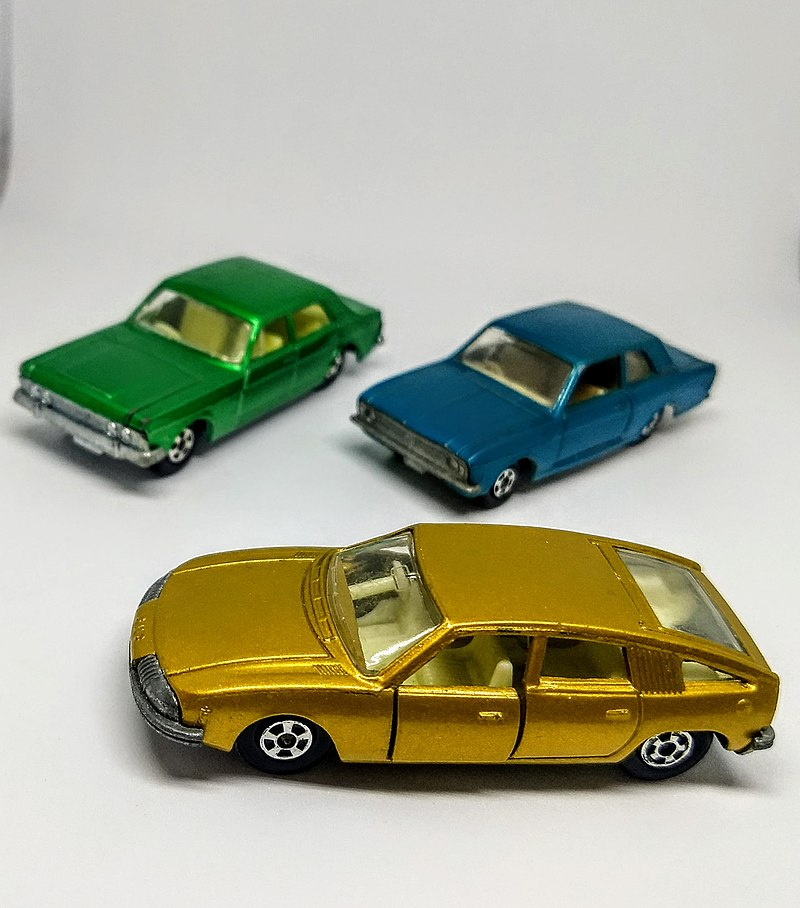
\includegraphics[width=0.25\linewidth,height=\textheight,keepaspectratio]{img/matchbox.jpg}

}

\caption{\label{fig-matchbox}Matchbox-Autos sind Modelle für Autos,
Spurzem (2017)}

\end{figure}%

\begin{definition}[Modelle]\protect\hypertarget{def-modelle}{}\label{def-modelle}

Modelle sind ein vereinfachtes Abbild der Realität, eine
\emph{Repräsentation} (Kaplan, 2009). \(\square\)

\end{definition}

\begin{example}[Beispiele für
Modelle]\protect\hypertarget{exm-Modelle}{}\label{exm-Modelle}

Puppen sind Modelle für Babies, Landkarten für Landstriche und das
Atommodell von Nils Bohr ist ein Modell für Atome. \(\square\)

\end{example}

Auch in der Statistik nutzen wir Modelle. Helfen Sie Prof.~Weiss-Ois: Er
blickt nicht durch, s. Beispiel~\ref{exm-weiss-ois}. Gerne würde er
wissen, wie viele Stunden seine Studentis auf die Prüfung lernen. Aber
mit so vielen Zahlen kann er nicht umgehen \ldots{} Geben Sie ihm ein
Modell: Sagen Sie ihm, wie lang die Studis typischerweise lernen (sagen
Sie ihm ein einfach den \emph{Mittelwert} der Lernzeiten, 9.6 Stunden).

\begin{example}[Prof Weiss-Ois blickt nicht
durch]\protect\hypertarget{exm-weiss-ois}{}\label{exm-weiss-ois}

~

\begin{quote}
{\emoji{teacher}} Vorher: 12, 8, 10, 11, 10, 9, 13, 9, 14, 9, 12, 14, 7,
9, 9, 11, 9, 4, 5, 12, 9, 6, 9, 12, 13, 9, 9, 6, 10\ldots{} Oh je, so
viele Zahlen! Ich check nix! Wie viel lernen denn jetzt meine Studis?!
\end{quote}

\begin{quote}
{\emoji{teacher}} Ah, 9.6 Stunden! Yeah, jetzt weiß ich, wie viel die
Studis so typischerweise lernen. Viel zu wenig natürlich!
\end{quote}

Prof.~I. Ch. Weiss-Ois hat den Mittelwert verstanden \ldots{}
\(\square\)

\end{example}

Der Nutzen von Modellen ist, dass sie komplexe Sachverhalte vereinfachen
und damit oft überhaupt erst dem Verständnis oder einer Untersuchung
zugänglich machen: Modelle ermöglichen Verständnis. In der Datenanalyse
bzw. Statistik (die beiden Begriffe werden hier weitgehend synonym
gebraucht) fassen Modelle oft viele Daten prägnant zusammen, z.B. zu
einer einzelnen Kennzahl. Das Verrückte an Modellen ist, dass man
Informationen wegwirft, um eine (andere, hoffentlich nützlichere)
Information zu bekommen (Stigler, 2016). Weniger ist mehr?!

\section{Praxisbezug}\label{praxisbezug}

Wir leben im Datenzeitalter; Daten durchdringen alle Bereiche des
beruflichen, gesellschaftlichen und privaten Lebens. Die Datenanalyse
hat sich in den letzten Jahren massiv verändert, da Datenmengen und
Methoden einen regelrechten Boom erlebt haben. Diese Entwicklung ist
durchaus auch kritisch zu betrachten; viele Menschen betrachten die
Entwicklung im Datenzeitalter -- Stichwort künstliche Intelligenz -- mit
Sorge. Egal ob man Daten als Segen oder Fluch betrachtet, in beiden
Fällen ist es wichtig, mit Daten umgehen zu können. Mit der wachsenden
Bedeutung von Daten wächst in gleichem Maße die Bedeutung von
Datenanalyse. Denn Daten ohne Sinn sind nutzlos. Aus diesem Grund kann
man sagen, dass Datenanalyse (und damit auch Statistik als eine
spezielle Art von Datenanalyse) zu stark nachgefragten Jobs gehören.

\section{Wie man mit Statistik
lügt}\label{wie-man-mit-statistik-luxfcgt}

Das \emph{File-Drawer-Problem}: Sie haben ein tolles Experiment
durchgeführt, viel Arbeit, viel Stress, endlich geschafft, puh. Von den
20 Variablen (als AV, s. Kapitel~\ref{sec-arten-variablen}), die Sie
untersucht haben, zeigt nur 1 einen interessanten Effekt, leider. 1 von
20, das hört sich nicht so toll an. Wäre es da nicht \enquote{elegant},
die 19 Variablen ohne schönen Effekt einfach in der Schublade liegen zu
lassen bis zum Sankt-Nimmerleins-Tag? Dann könnten Sie stattdessen als
Ergebnis nur die eine Variable mit schönen Ergebnis präsentieren, ganz
ohne widersprechende Befunde.

Dieser Versuchung nicht zu erliegen, kann schwer sein. Es ist aber
gefährlich, missliebige Ergebnisse zu verschweigen: Die anderen Menschen
bekommen dann ein falsches Bild der Ergebnislage; man spricht von
\href{https://de.wikipedia.org/wiki/Publikationsbias}{Publikationsbias}
(Marks-Anglin, Arielle and Chen, Yong, 2020). Wer Ergebnisse
verschweigt, verzerrt die gesamte Befundlage (Rothstein, 2014) -- ein
Fall von wissenschaftlichem Fehlverhalten.

\section{Fazit}\label{fazit-1}

Die Aufgabe von Statistik ist es, durch Zusammenfassen von Daten Modelle
zu bilden, die es uns einfacher machen, schwierige Sachverhalte zu
verstehen. Zentral ist dabei die Analyse von Variabilität der Daten.
Daten kommen in verschiedenen Varianten vor, typischerweise in
Tabellenform, möglichst im Tidy-Format.

\section{Aufgaben}\label{aufgaben}

Die Webseite \href{https://datenwerk.netlify.app}{datenwerk.netlify.app}
stellt eine Reihe von einschlägigen Übungsaufgaben bereit. Sie können
die Suchfunktion der Webseite nutzen, um die Aufgaben mit den folgenden
Namen zu suchen:

\begin{enumerate}
\def\labelenumi{\arabic{enumi}.}
\tightlist
\item
  \href{https://sebastiansauer.github.io/Datenwerk/posts/variation01/variation01.html}{variation01}
\item
  \href{https://sebastiansauer.github.io/Datenwerk/posts/def-statistik01/def-statistik01}{Def-Statistik01}
\item
  \href{https://sebastiansauer.github.io/Datenwerk/posts/tidy1/tidy1.html}{tidy1}
\item
  \href{https://sebastiansauer.github.io/Datenwerk/posts/skalenniveau1a/skalenniveau1a}{Skalenniveau1a}
\item
  \href{https://sebastiansauer.github.io/Datenwerk/posts/ziele-statistik/ziele-statistik}{Ziele-Statistik}
\item
  \href{https://sebastiansauer.github.io/Datenwerk/posts/variation02/variation02.html}{variation02}
\item
  \href{https://sebastiansauer.github.io/Datenwerk/posts/skalenniveau1b/skalenniveau1b}{Skalenniveau1b}
\item
  \href{https://sebastiansauer.github.io/Datenwerk/posts/tidydata1/tidydata1.html}{tidydata1}
\end{enumerate}

\section{Vertiefung}\label{vertiefung}

\subsection{Excel für Könner}\label{excel-fuxfcr-kuxf6nner}

In vielen Organisationen werden Exceltabellen für bestimmte Zwecke der
Datenverarbeitung verwendet. Excel und ähnliche Programme haben
bestimmte Stärken und Vorteile, aber auch gewisse Nachteile und
Schwäche; das liegt z.T. daran, dass Excel für bestimmte Aufgaben besser
und für andere weniger gut geeignet ist. Wenn man mit Excel arbeitet,
wiederholen sich erfahrungsgemäß immer wieder die gleichen Fehler bzw.
kommt es wiederholt zu einer suboptimalen Vorgehensweise zum Aufbau
einer Exceltabelle.

\href{https://www.tandfonline.com/doi/full/10.1080/00031305.2017.1375989}{Dieser
Artikel} von Broman \& Woo (2018) zeigt anhand einiger praktischer
Tipps, wie man Exceltabellen so aufbaut, dass Fehler minimiert werden.

\begin{exercise}[Fassen Sie den Artikel von Broman \& Woo (2018)
zusammen]\protect\hypertarget{exr-xls-paper}{}\label{exr-xls-paper}

Fassen Sie das \emph{Wesentliche} (und nur das Wesentliche) zum Artikel
zusammen. \(\square\)

\end{exercise}

\subsection{Sind Sie süchtig nach Ihrem
Handy?}\label{sind-sie-suxfcchtig-nach-ihrem-handy}

\begin{figure}

\begin{minipage}{0.80\linewidth}
Sind Sie süchtig nach Ihrem Handy? Lassen Sie uns eine kleine Studie
dazu (ggf. live im Hörsaal) durchführen. Füllen Sie
\href{https://forms.gle/PP8yb6Ubqq3JU78F9}{diese Umfrage} zum Thema
Smartphonse-Sucht aus (anonym und kein Muss).\end{minipage}%
%
\begin{minipage}{0.20\linewidth}

\begin{center}

\includegraphics[width=0.75\linewidth,height=\textheight,keepaspectratio]{010-rahmen_files/figure-pdf/qr-google-forms-handysucht-1.pdf}
\end{center}

\end{minipage}%

\end{figure}%

Kernstück der Umfrage ist die Smartphone-Sucht-Skala (Kwon et al.,
2013). Eine Studie fand, dass ca. ein Siebtel der Studierenden süchtig
nach ihrem Smartphone ist (Haug et al., 2015); demnach könnte dem Thema
eine hohe Bedeutsamkeit zukommen.

\section{Literaturhinweise}\label{literaturhinweise}

Einen Einblick in die Fundamente statistischer Analyse bietet Stigler
(2016). Cetinkaya-Rundel \& Hardin (2021) stellen grundlegende Konzepte
der Analyse von Daten im Kapitel 1, \enquote{Hello data}, vor. Downey
(2023) illustriert statistische Überraschungsmoment auf unterhaltsame,
und vor allem: sofataugliche Art.

\chapter{Daten einlesen}\label{sec-dateneinlesen}

\[
\definecolor{ycol}{RGB}{230,159,0}
\definecolor{modelcol}{RGB}{86,180,233}
\definecolor{errorcol}{RGB}{0,158,115}
\definecolor{beta0col}{RGB}{213,94,0}
\definecolor{beta1col}{RGB}{0,114,178}
\definecolor{xcol}{RGB}{204,121,167}
\]

\section{Einstieg}\label{einstieg-2}

Abb. Abbildung~\ref{fig-ueberblick} den Standort dieses Kapitels im
Lernpfad und gibt damit einen Überblick über das Thema dieses Kapitels
im Kontext aller Kapitel.

\subsection{Lernziele}\label{lernziele-2}

\begin{itemize}
\tightlist
\item
  Sie können R und RStudio starten.
\item
  Sie können R-Pakete installieren und starten.
\item
  Sie können Variablen in R zuweisen und auslesen.
\item
  Sie können Daten in R importieren.
\item
  Sie können den Begriff \emph{Reproduzierbarkeit} definieren.
\end{itemize}

\subsection{Ab diesem Kapitel benötigen Sie
R}\label{ab-diesem-kapitel-benuxf6tigen-sie-r}

Bitte stellen Sie sicher, dass Sie R rechtzeitig einsatzbereit haben.
Weiter unten in diesem Kapitel finden Sie Installationshinweise
(Kapitel~\ref{sec-install-r}). Falls Sie dieses Kapitel zum ersten Mal
bzw. sich noch nicht mit R auskennen, werden Sie vielleicht einigen
Inhalten begegnen, die Sie noch nicht gleich verstehen. Keine Sorge, das
ist normal. Mit etwas Übung wird Ihnen bald alles schnell von der Hand
gehen.

\section{Errrstkontakt}\label{errrstkontakt}

\subsection{Warum R?}\label{warum-r}

Gründe, die für den Einsatz von R sprechen:

\begin{enumerate}
\def\labelenumi{\arabic{enumi}.}
\item
  R ist kostenlos, andere Softwarepakete für Datenanalyse sind teuer.
\item
  R und R-Befehle sind quelloffen, d.h. man kann sich die
  zugrundeliegenden Computerbefehle anschauen. Jeder kann prüfen, ob R
  vernünftig arbeitet. Alle können beitragen.
\item
  R hat die neuesten Methoden.
\item
  R hat eine große Community.
\item
  R ist maßgeschneidert für Datenanalyse.
\end{enumerate}

Allerdings gibt es auch abweichende Meinungen, s.
Abbildung~\ref{fig-bill-excel}.

\begin{figure}

\centering{


\includegraphics[width=0.5\linewidth,height=\textheight,keepaspectratio]{img/bill-gates-excel.jpg}

}

\caption{\label{fig-bill-excel}Manche finden Excel cooler als R, nicht
wahr, Bill Gates? (imgflip, 2024a)}

\end{figure}%

\subsection{R und Reproduzierbarkeit}\label{r-und-reproduzierbarkeit}

\begin{definition}[Reproduzierbarkeit]\protect\hypertarget{def-repro}{}\label{def-repro}

Ein (wissenschaftlicher) Befunde ist reproduzierbar, wenn andere
Personen mit der Analysemethodik zum gleichen Ergebnis (wie in der
ursprünglichen Analyse) kommen (Plesser, 2018). \(\square\)

\end{definition}

Definition~\ref{def-repro} ist, etwas überspitzt, in
Abbildung~\ref{fig-repro} wiedergegeben.

\begin{figure}

\centering{


\includegraphics[width=0.5\linewidth,height=\textheight,keepaspectratio]{img/repro-star-struck.png}

}

\caption{\label{fig-repro}Daten + Syntax + genaue Beschreibung der
Messungen = reproduzierbar}

\end{figure}%

\begin{example}[Aus der Forschung: Reproduzierbarkeit in der
Psychologie]\protect\hypertarget{exm-repro}{}\label{exm-repro}

~

\begin{quote}
{\emoji{student}} Wie steht es um die Reproduzierbarkeit in der
Psychologie? Sind die Befunde zuverlässig?
\end{quote}

Obels et al. (2020) haben die Reproduzierbarkeit in psychologischen
Studien untersucht. Sie berichten folgendes Ergebnis (S. 229):

\begin{quote}
We examined data and code sharing for Registered Reports published in
the psychological literature from 2014 to 2018 and attempted to
independently computationally reproduce the main results in each
article. Of the 62 articles that met our inclusion criteria, 41 had data
available, and 37 had analysis scripts available. Both data and code for
36 of the articles were shared. We could run the scripts for 31
analyses, and we reproduced the main results for 21 articles.
\(\square\)
\end{quote}

\end{example}

\subsection{R \& RStudio}\label{r-rstudio}

Wenn wir sagen, \enquote{wir arbeiten mit R}, dann heißt das in unserem
Fall, wir arbeiten mit R und mit RStudio.

Ismay \& Kim (2020) zeigen in einer schönen Analogie, was den
Unterschied von \emph{R} und \emph{RStudio} ausmacht, s.
Abbildung~\ref{fig-r-rstudio}. (Streng genommen ist RStudio für die
Datenanalyse irrelevant, aber RStudio ist praktisch, Sie werden es nicht
missen wollen.)

\begin{figure}

\centering{

\pandocbounded{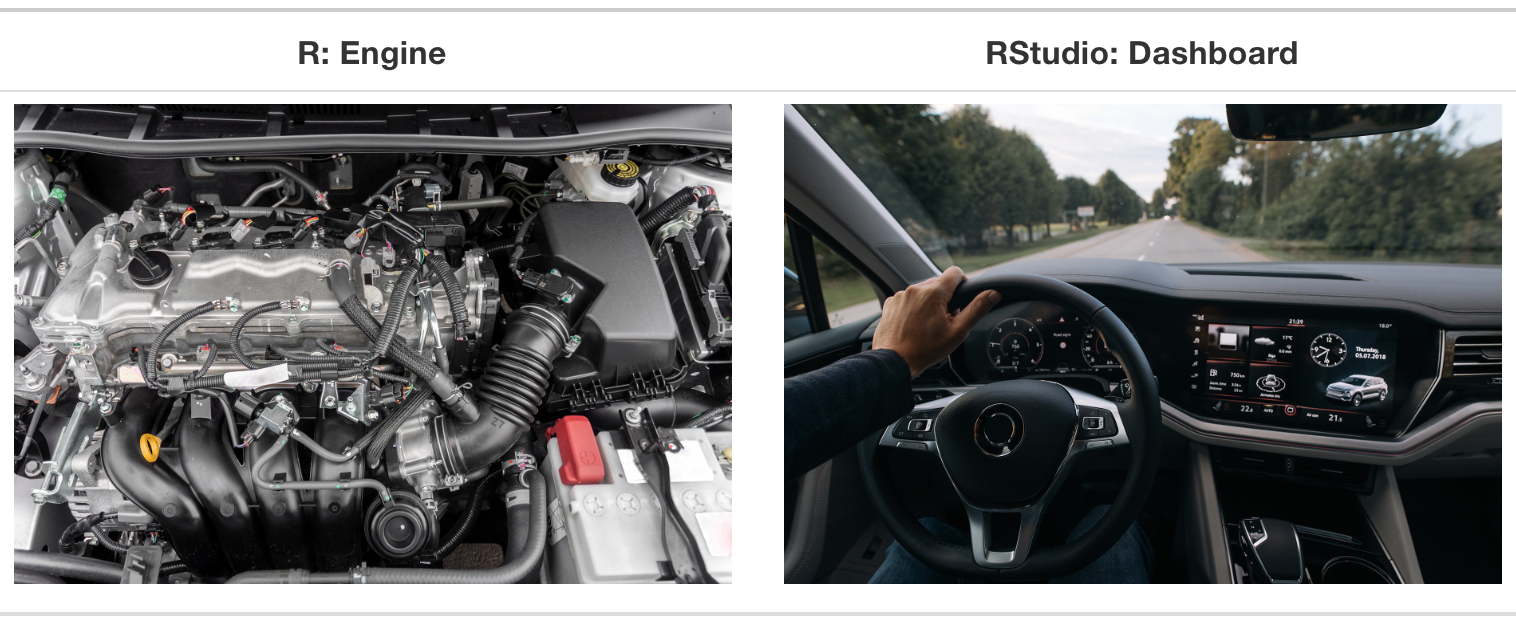
\includegraphics[keepaspectratio]{img/r_vs_rstudio_1.png}}

}

\caption{\label{fig-r-rstudio}R vs.~RStudio: R macht die Arbeit, RStudio
ist für Komfort und Übersicht (Ismay \& Kim, 2020).}

\end{figure}%

Kurz gesagt: Das eigentlich Arbeiten besorgt R. Für den Komfort und die
Schönheit ist RStudio zuständig. Auch eine Art von Arbeitsteilung!

\section{Installation von R und RStudio}\label{sec-install-r}

\subsection{Installation von R}\label{installation-von-r}

R ist ein Softwarepaket für statistische Berechnungen. Laden Sie es für
Ihr Betriebssytem herunter unter \url{https://cloud.r-project.org}.

Wenn Sie beim Herunterladen gefragt werden, dass Sie einen
\enquote{Mirror} auswählen sollen, heißt das, Sie sollen einen Computer
(Server) wählen, von dem Sie R herunterladen. Der sollte möglichst nicht
zu weit weg stehen, dann spart es vielleicht etwas Zeit und Bandbreite.

Wenn Sie die Installationsdatei heruntergeladen haben, öffnen Sie diese
Datei (Doppelklick) und Sie werden durch die Installation geführt. (Sie
benötigen Admin-Rechte auf Ihrem Computer.)

\subsection{Installation von RStudio
Desktop}\label{installation-von-rstudio-desktop}

RStudio ist eine \emph{graphische Benutzeroberfläche} (graphical user
interface, GUI) für R, plus ein paar Goodies (in Form einer
\emph{intergrierten Entwicklungsumgebung} (integrated development
environment, IDE). Laden Sie die \emph{Desktop-Version} von RStudio
herunter für Ihr Betriebssystem (Windows, MacOS, Linux) vom Anbieter
(Posit) herunter.\footnote{\url{https://posit.co/download/rstudio-desktop/}}
Wenn Sie die Installationsdatei heruntergeladen haben, öffnen Sie diese
Datei (Doppelklick) und Sie werden durch die Installation geführt. (Sie
benötigen u. U. Admin-Rechte auf Ihrem Computer.)

\subsection{Posit/RStudio Cloud}\label{positrstudio-cloud}

Posit Cloud bzw. RStudio Cloud (\url{https://rstudio.cloud/}) ist ein
Webdienst von Posit (zum Teil kostenlos), also ein \emph{RStudio
online}: Man kann damit online mit R arbeiten. Sie können es als
Alternative zur Installation von RStudio auf Ihrem Computer verwenden.
Ein Vorteil von RStudio Cloud ist, dass man als Nutzer \emph{nichts
installieren} muss und dass es \emph{auch auf Tablets} läuft (im
Gegensatz zur Desktop-Version von RStudio). Ein Nachteil ist, dass es
etwas langsamer ist und nur für ein gewisses Zeitvolumen kostenlos. Sie
müssen sich erst ein Konto beim Anbieter anlegen, um den Dienst nutzen
zu können.

\subsubsection{Vertiefung}\label{vertiefung-1}

Wenn Ihnen jemand (z.B. eine Lehrkraft) einen
RStudio-Cloud-Projektordner bzw. einen Link dazu bereitstellt, ist das
komfortabel, da die Lehrkraft dann schon Pakete installieren, Daten
bereitstellen und andere Nettigkeit vorbereiten kann für Sie. Allerdings
müssen Sie den Projektordner in Ihrem eigenen Konto abspeichern, wenn
Sie etwas speichern möchten, da Sie vermutlich keine Schreibrechte im
Projektordner dieser nettern Person (Ihrer Lehrkraft) haben. Klicken Sie
dazu auf \enquote{Save a permanent copy}, s.
Abbildung~\ref{fig-perm-copy}.

\begin{figure}

\centering{

\pandocbounded{
\includegraphics[keepaspectratio]{img/rstudio-save-a-permanent-copy.png}}

}

\caption{\label{fig-perm-copy}Einen Projektordner im eigenen Konto
abspeichern, um Schreibrechte zu haben}

\end{figure}%

Sie können auch von der Cloud exportieren, also Ihre Syntaxdatei
herunterladen. Klicken Sie dazu im Reiter \enquote{Files} auf
\texttt{More\ \textgreater{}\ Export}.

\begin{tcolorbox}[enhanced jigsaw, leftrule=.75mm, breakable, left=2mm, colback=white, colframe=quarto-callout-note-color-frame, opacitybacktitle=0.6, coltitle=black, colbacktitle=quarto-callout-note-color!10!white, arc=.35mm, bottomtitle=1mm, toprule=.15mm, rightrule=.15mm, toptitle=1mm, titlerule=0mm, title=\textcolor{quarto-callout-note-color}{\faInfo}\hspace{0.5em}{Hinweis}, bottomrule=.15mm, opacityback=0]

RStudio starten, nicht R. \(\square\)

\end{tcolorbox}

Wir verwenden beide Programme (R und RStudio). Aber wir \emph{öffnen
nur} RStudio. RStudio findet selbständig R und öffnet dieses
\enquote{heimlich}. Öffnen Sie nicht noch extra R (sonst wäre R zweifach
geöffnet). Anstelle von \emph{RStudio Desktop} (auf Ihrem
Computer/Desktop) können Sie auch die \emph{RStudio Cloud} (die
Online-Version) starten

\section{R-Pakete}\label{r-pakete}

\subsection{Was sind R-Pakete?}\label{was-sind-r-pakete}

Typisch für R ist sein modularer Aufbau: Man kann eine große Zahl an
Erweiterungen (\enquote{Pakete}, engl. \emph{packages}) installieren,
alle kostenlos. In R Paketen \enquote{wohnen} R-Befehle, also Dinge, die
R kann, \enquote{Skills} sozusagen. Außerdem können in R-Paketen auch
Daten bereitgestellt werden. Damit man die Inhalte eines R-Pakets nutzen
kann, muss man es zuerst installieren und dann verfügbar machen
(\enquote{starten}). Man kann sich daher ein R-Paket vorstellen wie ein
Buch: Wenn R es gelesen hat, dann kennt es die Inhalte. Diese Inhalte
könnten irgendwelche Formeln, also Berechnungen sein. Es könnte aber die
\enquote{Bauanleitung} für ein schönes Diagramm sein. Ist ein spezielles
R-Paket auf Ihrem Computer installiert, so können Sie diese
Funktionalität nutzen.

Die Anzahl der R-Pakete ist groß; allein auf dem \enquote{offiziellen
Web-Store} (nennt sich \enquote{CRAN}) von R gibt es ca. 20,000 Pakete
(Hornik et al., 2023). Und es kommen immer mehr dazu.

\subsection{Pakete installieren}\label{sec-install-r-pckgs}

Wie jede Software muss man Pakete (Erweiterungen für R) erst einmal
installieren, bevor man sie verwenden kann. Übrigens, \emph{einmal}
installieren reicht. Das Installieren geht komfortabel, wenn man beim
Reiter \emph{Packages} auf \emph{Install} klickt und dann den Namen des
zu installierenden Pakets eingibt.

\begin{quote}
{\emoji{student}} Welche R-Pakete sind denn schon installiert?
\end{quote}

Im Reiter \emph{Packages} können Sie nachschauen, welche Pakete auf
Ihrem Computer schon installiert sind.

Alternativ können Sie zum Installieren von Paketen auch den Befehl
\texttt{install.packages()} verwenden. Also zum Beispiel
\texttt{install.packages(tidyverse)}, um das Paket \texttt{tidyverse} zu
installieren.

\begin{quote}
{\emoji{student}} Ja, aber welche R-Pakete \enquote{soll} ich denn
installieren, welche brauche ich denn?
\end{quote}

Im Moment sollten Sie die folgenden Pakete installiert haben:

\begin{itemize}
\tightlist
\item
  \texttt{tidyverse}
\item
  \texttt{easystats}
\end{itemize}

Wenn Sie die noch nicht installiert haben sollten, dann können Sie das
jetzt ja nachholen. (Übrigens sind \texttt{tidyverse} und
\texttt{easystats} Pakete, die nur dafür da sind, mehrere Pakete zu
installieren. So gehören z.B. zu \texttt{tidyverse} die Pakete
\texttt{ggplot} (Daten verbildlichen) und \texttt{dplyr} (Datenjudo).
Damit wir nicht alle Pakete einzeln installieren und starten müssen,
bietet uns das Paket \texttt{tidyverse} den Komfort, alle die Pakete
dieser \enquote{Sammlung} auf einmal zu starten. Praktisch.)

\begin{tcolorbox}[enhanced jigsaw, leftrule=.75mm, breakable, left=2mm, colback=white, colframe=quarto-callout-caution-color-frame, opacitybacktitle=0.6, coltitle=black, colbacktitle=quarto-callout-caution-color!10!white, arc=.35mm, bottomtitle=1mm, toprule=.15mm, rightrule=.15mm, toptitle=1mm, titlerule=0mm, title=\textcolor{quarto-callout-caution-color}{\faFire}\hspace{0.5em}{Vorsicht}, bottomrule=.15mm, opacityback=0]

Bevor Sie ein R-Paket (oder überhaupt irgendwelche Software)
installieren/updaten, sollten Sie das entsprechende R-Paket
schließen/beenden. Sonst schrauben Sie sozusagen an einem elektrischen
Gerät herum, das noch unter Strom steht (nicht gut). Die einfachste Art,
alle Pakete zu beenden ist, \texttt{Session\ \textgreater{}\ Restart\ R}
zu klicken (in RStudio). \(\square\)

\end{tcolorbox}

\subsection{Pakete starten}\label{pakete-starten}

Wenn Sie ein Softwareprogramm installiert haben, müssen Sie es noch
\emph{starten}. Sie erkennen leicht, ob ein Paket bereitgestellt
(gestartet) ist, wenn Sie ein Häkchen vor dem Namen des Pakets in der
Paketliste (Reiter \emph{Packages}) sehen. Ein bestimmtes R-Paket muss
man nur \emph{einmalig installieren}. Aber man muss es \emph{jedes Mal
neu starten}, wenn man R (bzw. RStudio) startet.

\section{Mit R arbeiten}\label{mit-r-arbeiten}

\subsection{Projekte in R}\label{projekte-in-r}

Ein \emph{Projekt} in RStudio ist letztlich ein Ordner, der als
\enquote{Basis} für eine Reihe von zusammengehörigen Dateien verwendet
wird. Sagen wir, Sie nennen Ihr Projekt \texttt{cool\_stuff}. RStudio
legt uns diesen Ordner an einem von uns gewählten Platz auf unserem
Computer an. Das ist ganz praktisch, weil man dann sagen kann
\enquote{Hey R, nimmt die Datei \enquote*{daten.csv}}, ohne einen Pfad
anzugeben. Vorausgesetzt, die Datei liegt auch im Projektordner
(\texttt{cool\_stuff}). RStudio-Projekte kann anlegen mit Klick auf das
Icon, das einen Quader mit dem Buchstaben R darin anzeigen. Nutzen Sie
RStudio-Projekte, das macht Ihr Leben leichter. RStudio-Projekte zu
nutzen ist viel sicherer als das Arbeitsverzeichnis von Hand zu wählen
oder mit Pfaden herumzubasteln.

\subsection{Skriptdateien}\label{skriptdateien}

Die R-Befehle (\enquote{Syntax}) schreiben Sie am besten in eine
speziell dafür vorgesehene Textdatei in RStudio. Eine Sammlung von
(R-)Computer-Befehlen nennt man auch ein \emph{Skript}, daher spricht
man bei Dateien, die Syntax enthalten, von einer \emph{Skriptdatei}.

Um eine neue R-Skriptdatei zu erstellen, gibt es mehrere Wege. Einer
ist: klicken Sie auf das Icon, das ein weißes Blatt mit einem grünen
Pluszeichen zeigt, s. Abbildung~\ref{fig-script-new}.

\begin{figure}

\begin{minipage}{0.48\linewidth}

\centering{


\includegraphics[width=0.5\linewidth,height=\textheight,keepaspectratio]{img/script-new.png}

}

\subcaption{\label{fig-script-new1}Klick auf Icon}

\end{minipage}%
%
\begin{minipage}{0.05\linewidth}
~\end{minipage}%
%
\begin{minipage}{0.48\linewidth}

\centering{

\pandocbounded{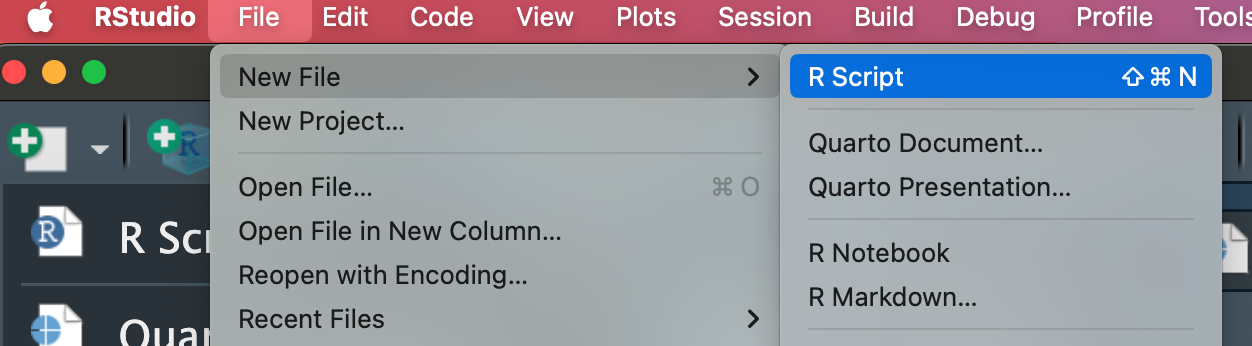
\includegraphics[keepaspectratio]{img/neue-skriptdatei.png}}

}

\subcaption{\label{fig-script-new2}Auswahl im Menu}

\end{minipage}%

\caption{\label{fig-script-new}Es gibt verschiedene Wege, um eine neue
R-Skript-Datei in RStudio zu öffnen. (a) Per Klick auf das Icon. (b) Im
Menü \texttt{File}, dann \texttt{R\ Script}.}

\end{figure}%

Vergessen Sie nicht zu \emph{speichern}, wenn Sie ein tolles Skript
geschrieben haben. Dafür gibt es mehrere Möglichkeiten:

\begin{enumerate}
\def\labelenumi{\arabic{enumi}.}
\tightlist
\item
  Tastaturkürzel \emph{Strg+S}
\item
  Menü: \texttt{File\ \textgreater{}\ Save}
\item
  Klick auf das Icon mit der Diskette, s.
  Abbildung~\ref{fig-script-new}.
\end{enumerate}

Eine existierende Skriptdatei können Sie in typischer Manier
\emph{öffnen}:

\begin{enumerate}
\def\labelenumi{\arabic{enumi}.}
\tightlist
\item
  Strg+O
\item
  Klick auf das Icon mit der Akte und dem grünen Pfeil (vgl.
  Abbildung~\ref{fig-script-new})
\item
  Menü: \texttt{File\ \textgreater{}\ Open\ File...}
\end{enumerate}

\subsection{Quarto-Dokumente}\label{quarto-dokumente}

\href{https://quarto.org/}{Quarto}\footnote{\url{https://quarto.org/}}
ist ein Programm zum Erstellen von Texten, in die man R-Syntax einfügen
kann. Die Ausgaben der R-Befehle werden dann direkt im Dokument
eingebunden. Quarto ist in RStudio integriert. Quarto ist eine
komfortable und leistungsfähige Methode, um Dokumente mit R-Syntax zu
schreiben. Sie sind aber nicht verpflichtet, Quarto zu nutzen.
Stattdessen können Sie Ihre Syntax auch in Skriptdateien schreiben.

Wenn Sie Quarto nutzen möchten, müssen Sie es zunächst installieren,
d.h. herunterladen. Dann können Sie in RStudio Quarto-Dateien erstellen.
Ein neues Quarto-Dokument können Sie erstellen mit Klick auf \emph{File
\textgreater{} New File \textgreater{} Quarto Document}.

\section{Errisch für Einsteiger}\label{errisch-fuxfcr-einsteiger}

\subsection{Variablen}\label{sec-rvars}

In jeder Programmiersprache kann man Variablen definieren, so auch in R:

\begin{Shaded}
\begin{Highlighting}[]
\NormalTok{richtige\_antwort }\OtherTok{=} \DecValTok{42}
\NormalTok{falsche\_antwort }\OtherTok{=} \DecValTok{43}
\NormalTok{typ }\OtherTok{=} \StringTok{"Antwort"}
\NormalTok{ist\_korrekt }\OtherTok{=} \ConstantTok{TRUE}
\end{Highlighting}
\end{Shaded}

Alternativ zum Gleichheitszeichen \texttt{=} können Sie auch (synonym)
den Zuweisungspfeil \texttt{\textless{}-} verwenden. Beides führt zum
gleichen Ergebnis. Allerdings ist der Zuweisungspfeil präziser, und
sollte daher \emph{bevorzugt} werden.

Der \emph{Zuweisungspfeil} \texttt{\textless{}-} bzw. das
Gleichheitszeichen \texttt{=} definiert eine neue \emph{Variable} (oder
überschreibt den Inhalt, wenn die Variable schon existiert).

\begin{Shaded}
\begin{Highlighting}[]
\NormalTok{richtige\_antwort }\OtherTok{\textless{}{-}} \DecValTok{42}
\NormalTok{falsche\_antwort }\OtherTok{\textless{}{-}} \DecValTok{43}
\NormalTok{typ }\OtherTok{\textless{}{-}} \StringTok{"Antwort"}
\NormalTok{ist\_korrekt }\OtherTok{\textless{}{-}} \ConstantTok{TRUE}
\end{Highlighting}
\end{Shaded}

Sie können sich eine Variable wie einen Becher oder Behälter vorstellen,
der bestimmte Werte enthält, z.B. den Wert \enquote{9° Celsius}. Auf dem
Becher steht der Name des Bechers geschrieben, z.B.
\enquote{Temperatur}. Natürlich können Sie die Werte aus dem Becher
entfernen und sie durch neue ersetzen (vgl.
Abbildung~\ref{fig-def-vars}).

\begin{figure}

\centering{

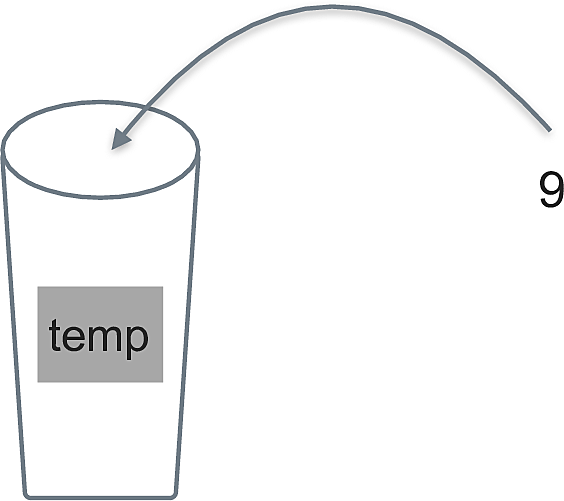
\includegraphics[width=0.25\linewidth,height=\textheight,keepaspectratio]{img/Variablen_zuweisen.png}

}

\caption{\label{fig-def-vars}Variablen zuweisen: Der Variable mit dem
Namen \texttt{temp} weisen wir den Wert \texttt{9} zu.}

\end{figure}%

R kann übrigens auch rechnen. Probieren Sie es doch gleich mal hier aus!

\begin{Shaded}
\begin{Highlighting}[]
\NormalTok{die\_summe }\OtherTok{\textless{}{-}}\NormalTok{ falsche\_antwort }\SpecialCharTok{+}\NormalTok{ richtige\_antwort}
\end{Highlighting}
\end{Shaded}

Aber was ist jetzt der Wert, der \enquote{Inhalt} der Variable
\texttt{die\_summe}?

Um den Wert, d.h. den Inhalt einer Variablen in R \emph{auszulesen},
geben wir einfach den Namen des Objekts ein:

\begin{Shaded}
\begin{Highlighting}[]
\NormalTok{die\_summe}
\DocumentationTok{\#\# [1] 85}
\end{Highlighting}
\end{Shaded}

Was passiert wohl, wenn wir \texttt{die\_summe} jetzt wie folgt
definieren?

\begin{Shaded}
\begin{Highlighting}[]
\NormalTok{die\_summe }\OtherTok{\textless{}{-}}\NormalTok{ falsche\_antwort }\SpecialCharTok{+}\NormalTok{ richtige\_antwort }\SpecialCharTok{+} \DecValTok{1}
\end{Highlighting}
\end{Shaded}

Wer hätt's geahnt:

\begin{Shaded}
\begin{Highlighting}[]
\NormalTok{die\_summe}
\DocumentationTok{\#\# [1] 86}
\end{Highlighting}
\end{Shaded}

Variablen können auch \enquote{leer} sein:

\begin{Shaded}
\begin{Highlighting}[]
\NormalTok{alter }\OtherTok{\textless{}{-}} \ConstantTok{NA}  \CommentTok{\# NA wie "not available", nicht vorhanden}
\NormalTok{alter}
\DocumentationTok{\#\# [1] NA}
\end{Highlighting}
\end{Shaded}

\texttt{NA} steht für \emph{not available}, nicht verfügbar und macht
deutlich, dass hier ein Wert fehlt.

\begin{quote}
{\emoji{student}} Wozu brauche ich bitte fehlende Werte?!
\end{quote}

Fehlende Werte sind ein häufiges Problem in der Praxis. Vielleicht hat
sich die befragte Person geweigert, ihr Alter anzugeben (Datenschutz!).
Oder als Sie die Daten in Ihren Computer eingeben wollten, ist Ihre
Katze über die Tastatur gelaufen und alles war futsch\ldots{}

\subsection{\texorpdfstring{Funktionen
(\enquote{Befehle})}{Funktionen (``Befehle'')}}\label{funktionen-befehle}

Das, was R kann, ist in \enquote{Funktionen} hinterlegt. Genauer gesagt
ist ein \enquote{Befehl} an R eine Funktion.

\begin{definition}[Funktion]\protect\hypertarget{def-fun}{}\label{def-fun}

Eine Funktion ist eine Regel, die jedem Eingabewert (auch Argument
genannt) einen Ausgabewert zuordnet. Man kann sich Funktionen als
Maschinen vorstellen, die Eingabedaten in Ausgabedaten umwandeln, vgl.
Abbildung~\ref{fig-function-schema}. \(\square\)

\end{definition}

Ein Beispiel für eine solche Funktion könnte sein: \enquote{Berechne den
Mittelwert dieser Datenreihe} (schauen wir uns gleich an). Das geht so:

\begin{Shaded}
\begin{Highlighting}[]
\NormalTok{Antworten }\OtherTok{\textless{}{-}} \FunctionTok{c}\NormalTok{(}\DecValTok{42}\NormalTok{, }\DecValTok{43}\NormalTok{)}
\end{Highlighting}
\end{Shaded}

Der Befehl \texttt{c} (c wie \emph{c}ombine) fügt mehrere Werte zusammen
zu einer \enquote{Liste} (einem Vektor). (Streng genommen sollte man
nicht von einer Liste sprechen, da es in R noch einen anderen Objekttyp
gibt, der \texttt{list} heißt, und eine verallgemeinerte Form eines
Vektors ist.)

\begin{definition}[Vektor]\protect\hypertarget{def-vektor}{}\label{def-vektor}

Als \emph{Vektor} (Datenreihe) bezeichnen wir eine geordnete Folge von
Werten. In R kann man sie mit der Funktion \texttt{c} erstellen. Die
Werte eines Vektors bezeichnet man als \emph{Elemente}. \(\square\)

\end{definition}

Mit dem Zuweisungspfeil geben wir diesem Vektor einen Namen, hier
\texttt{Antworten}. Dieser Vektor besteht aus zwei Werten, zuerst
\texttt{42}, dann kommt \texttt{43}.

\begin{example}[Beispiele für
Vektoren]\protect\hypertarget{exm-vektoren}{}\label{exm-vektoren}

Vektoren können (praktisch) beliebig lang sein, z.B. drei Elemente.

\begin{Shaded}
\begin{Highlighting}[]
\NormalTok{x }\OtherTok{\textless{}{-}} \FunctionTok{c}\NormalTok{(}\DecValTok{1}\NormalTok{, }\DecValTok{2}\NormalTok{, }\DecValTok{3}\NormalTok{)}
\NormalTok{y }\OtherTok{\textless{}{-}} \FunctionTok{c}\NormalTok{(}\DecValTok{2}\NormalTok{, }\DecValTok{1}\NormalTok{, }\DecValTok{3}\NormalTok{)  }\CommentTok{\# x und y sind ungleich (Reihenfolge der Werte)}
\NormalTok{z }\OtherTok{\textless{}{-}} \FunctionTok{c}\NormalTok{(}\FloatTok{3.14}\NormalTok{, }\FloatTok{2.71}\NormalTok{)  }
\NormalTok{namen }\OtherTok{\textless{}{-}} \FunctionTok{c}\NormalTok{(}\StringTok{"Anni"}\NormalTok{, }\StringTok{"Bert"}\NormalTok{, }\StringTok{"Charlie"}\NormalTok{) }\CommentTok{\# Text{-}Vektor}
\end{Highlighting}
\end{Shaded}

\end{example}

Zwei wichtige Typen von Vektoren sind numerische Vektoren (reelle
Zahlen; in R auch als \emph{numeric} oder \emph{double} bezeichnet) und
Textvektoren, in R auch als \emph{String} oder \emph{character}
bezeichnet.

\begin{example}[]\protect\hypertarget{exm-funs}{}\label{exm-funs}

Weitere Beispiel für Funktionen sind:

\begin{itemize}
\tightlist
\item
  \enquote{Erstelle eine Liste (Vektor) von Werten}.
\item
  \enquote{Lade dieses R-Paket.}
\item
  \enquote{Gib den größten Wert dieser Datenreihe aus.} \(\square\)
\end{itemize}

\end{example}

\subsection{Unsere erste statistische Funktion}\label{sec-first-fun}

Jetzt wird's ernst. Jetzt kommt die Statistik. Berechnen wir also unsere
erste statistische Funktion: Den Mittelwert. Puh.

\begin{Shaded}
\begin{Highlighting}[]
\FunctionTok{mean}\NormalTok{(Antworten)}
\DocumentationTok{\#\# [1] 42}
\end{Highlighting}
\end{Shaded}

Sie hätten \texttt{Antworten} auch durch \texttt{c(42,\ 43)} ersetzen
können, so haben Sie ja schließlich die Variable gerade definiert.

R arbeitet so einen \enquote{verschachtelten} Befehl \emph{von innen
nach außen} ab:

Start: \texttt{mean(Antworten)}

{\(\downarrow\)}

Schritt 1: \texttt{mean(c(42,\ 43))}

{\(\downarrow\)}

Schritt 2: \texttt{42.5}

Abbildung~\ref{fig-function-schema} stellt eine Funktion schematisch
dar.

\begin{figure}

\centering{

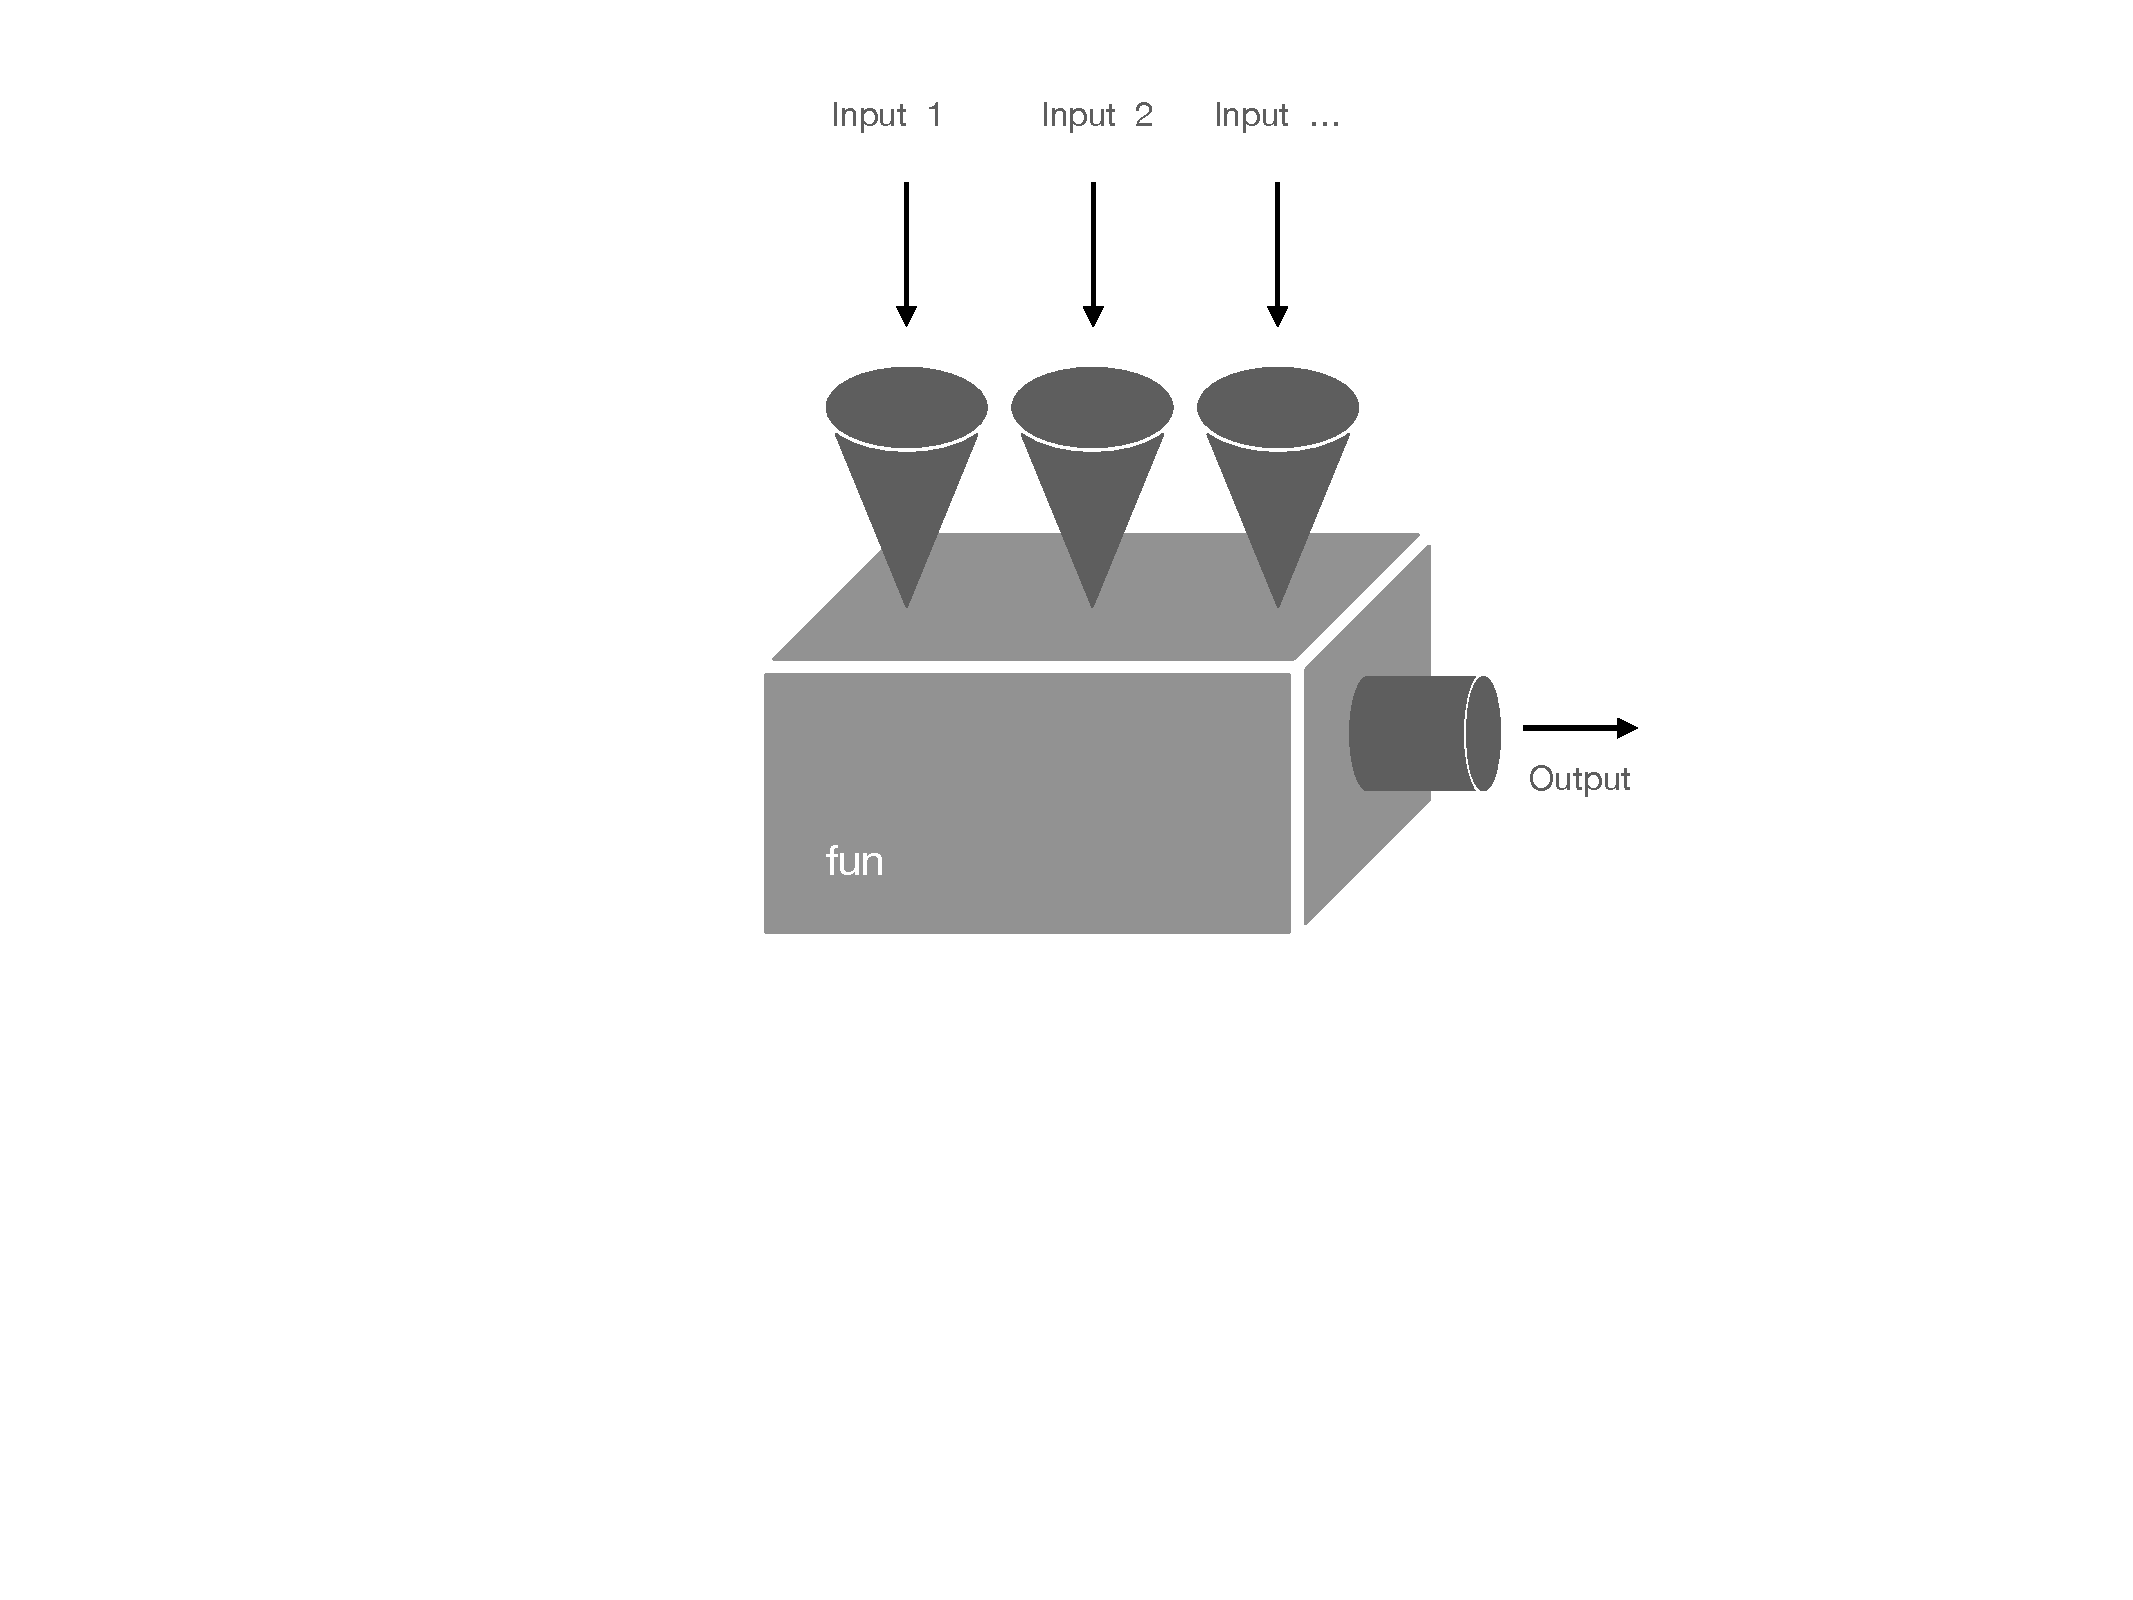
\includegraphics[width=0.75\linewidth,height=\textheight,keepaspectratio]{img/function-schema.pdf}

}

\caption{\label{fig-function-schema}Schema einer Funktion}

\end{figure}%

Eine Funktion hat einen oder mehrere \emph{Inputs} (s.
Abbildung~\ref{fig-function-schema}), das sind Daten oder
Verarbeitungshinweise, die man in die Funktion \texttt{fun}
\emph{eingibt}, bevor sie loslegt. Eine Funktion hat immer (genau) eine
\emph{Ausgabe} (Output), in der das Ergebnis einer Funktion ausgegeben
wird.

\begin{definition}[Argumente einer
Funktion]\protect\hypertarget{def-args}{}\label{def-args}

Die \enquote{Trichter} einer (R-)Funktion, in denen man die Eingaben
\enquote{einfüllt}, nennt man auch \emph{Argumente}. \(\square\)

\end{definition}

So hat die Funktion \texttt{mean} z.B. folgende Argumente, s.
Listing~\ref{lst-mean}.

\begin{codelisting}

\caption{\label{lst-mean}Die Argumente der R-Funktion \texttt{mean}}

\centering{

\begin{Shaded}
\begin{Highlighting}[]
\FunctionTok{mean}\NormalTok{(x, }\AttributeTok{trim =} \DecValTok{0}\NormalTok{, }\AttributeTok{na.rm =} \ConstantTok{FALSE}\NormalTok{, ...)}
\end{Highlighting}
\end{Shaded}

}

\end{codelisting}%

\begin{itemize}
\tightlist
\item
  \texttt{x}: das ist der Vektor, für den der Mittelwert berechnet
  werden soll
\item
  \texttt{trim\ =\ 0}: Sollen die extremsten Werte von \texttt{x} lieber
  \enquote{abgeschnitten} werden, also nicht in die Berechnung des
  Mittelwerts einfließen?
\item
  \texttt{na.rm\ =\ FALSE}: Wie soll mit fehlenden Werten \texttt{NA}
  umgegangen werden? Im Standard liefert \texttt{mean} (und viele andere
  arithmetische Funktionen in R) \texttt{NA} zurück. R schwenkt
  sozusagen die rote Fahne, um zu signalisieren: Achtung, Mensch, hier
  ist irgendwas nicht in Ordnung. Setzt man aber
  \texttt{na.rm\ =\ TRUE}, dann entfernt (remove, rm) R die fehlenden
  Werte und berechnet den Mittelwert, ohne weitere Hinweise zu den
  fehlenden Werten.
\item
  \texttt{...} heißt \enquote{sonstiges Zeugs, das manchmal eine Rolle
  spielen könnte}; darum kümmern wir uns jetzt nicht.
\end{itemize}

Einige Argumente haben einen \emph{Standardwert} bzw. eine
\emph{Voreinstellung} (engl. \emph{default}). So wird bei der Funktion
\texttt{mean} im Standard nicht getrimmt (\texttt{trim\ =\ 0}) und
fehlende Werte werden nicht entfernt (\texttt{na.rm\ =\ FALSE)}.

Wenn ein R-Befehl ein Argument mit Voreinstellung hat, brauchen Sie
dieses Argument \emph{nicht} zu befüllen. In dem Fall wird auf den Wert
der Voreinstellung zurückgegriffen. Argumente ohne Voreinstellung -- wie
\texttt{x} bei \texttt{mean} -- müssen Sie aber auf jeden Fall mit einem
Wert befüllen. Man würde also \texttt{mean} zumeist so aufrufen:
\texttt{mean(x)}.

Bei jedem R-Befehl haben die Argumente eine bestimmte Reihenfolge, etwa
bei \texttt{mean}:
\texttt{mean(x,\ trim\ =\ 0,\ na.rm\ =\ FALSE,\ ...)}.

(Nur) wenn man die Argumente in ihrer vorgegebenen Reihenfolge
anspricht, muss man \emph{nicht} den Namen des Arguments anführen:

\emoji{check-mark-button} \texttt{mean(Antworten,\ 0,\ FALSE)}

Hält man sich aber nicht an die vorgebene Reihenfolge, so weiß R nicht,
was zu tun ist und flüchtet sich in eine Fehlermeldung:

\begin{Shaded}
\begin{Highlighting}[]
\FunctionTok{mean}\NormalTok{(Antworten, }\ConstantTok{FALSE}\NormalTok{, }\DecValTok{0}\NormalTok{)  }\CommentTok{\# FALSCH, DON\textquotesingle{}T DO IT }
\DocumentationTok{\#\# Error in mean.default(Antworten, FALSE, 0): \textquotesingle{}trim\textquotesingle{} must be numeric of length one}
\end{Highlighting}
\end{Shaded}

Wenn man die Namen der Argumente anspricht, ist die Reihenfolge egal:

\begin{Shaded}
\begin{Highlighting}[]
\FunctionTok{mean}\NormalTok{(}\AttributeTok{na.rm =} \ConstantTok{FALSE}\NormalTok{, }\AttributeTok{x =}\NormalTok{ Antworten)  }\CommentTok{\# ok}
\FunctionTok{mean}\NormalTok{(}\AttributeTok{trim =} \DecValTok{0}\NormalTok{, }\AttributeTok{x =}\NormalTok{ Antworten, }\AttributeTok{na.rm =} \ConstantTok{TRUE}\NormalTok{)  }\CommentTok{\# ok}
\end{Highlighting}
\end{Shaded}

Übrigens: Leerzeichen sind R fast immer egal. Aus Gründen der
Übersichtlichkeit sollte man aber Leerzeichen verwenden. In diesen
Fällen sind Leerzeichen nicht erlaubt:

\begin{itemize}
\tightlist
\item
  \texttt{\textless{}-}
\item
  \texttt{\textless{}=} etc.
\item
  Variablennamen
\end{itemize}

\subsection{Vorsicht bei fehlenden
Werten}\label{vorsicht-bei-fehlenden-werten}

Sagen wir, wir haben einen fehlenden Wert in unseren Daten:

\begin{Shaded}
\begin{Highlighting}[]
\NormalTok{Antworten }\OtherTok{\textless{}{-}} \FunctionTok{c}\NormalTok{(}\DecValTok{42}\NormalTok{, }\DecValTok{43}\NormalTok{, }\ConstantTok{NA}\NormalTok{)}
\NormalTok{Antworten}
\DocumentationTok{\#\# [1] 42 43 NA}
\end{Highlighting}
\end{Shaded}

Wenn wir jetzt den Mittelwert berechnen wollen, quittiert R das mit
einem schnöden \texttt{NA}. \texttt{NA} steht für \emph{not available},
ist also ein Hinweis, dass Werte fehlen.

\begin{Shaded}
\begin{Highlighting}[]
\FunctionTok{mean}\NormalTok{(Antworten)}
\DocumentationTok{\#\# [1] NA}
\end{Highlighting}
\end{Shaded}

R meint es gut mit Ihnen\footnote{{\emoji{robot}} Naja, manchmal.}.
Stellen Sie sich vor, dass R Sie auf dieses Problem aufmerksam machen
möchte:

\begin{quote}
{\emoji{robot}} Achtung, NAs, fehlende Werte, lieber Herr und Gebieter,
du hast nicht mehr alle Latten am Zaun, will sagen, alle Daten im
Vektor!
\end{quote}

(Danke, R.)

Möchten Sie aber lieber R dieses Verhalten austreiben, so befüllen Sie
das Argument \texttt{na.rm} mit dem Wert \texttt{TRUE} (\texttt{na.rm}
steht für \emph{r}e\emph{m}ove die NA, also fehlenden Werte).

\begin{Shaded}
\begin{Highlighting}[]
\FunctionTok{mean}\NormalTok{(Antworten, }\AttributeTok{na.rm =} \ConstantTok{TRUE}\NormalTok{)}
\DocumentationTok{\#\# [1] 42}
\end{Highlighting}
\end{Shaded}

\subsection{Vektorielles Rechnen}\label{sec-veccalc}

\begin{definition}[Vektorielles
Rechnen]\protect\hypertarget{def-veccalc}{}\label{def-veccalc}

Das Rechnen mit Vektoren in R bezeichnen wir als \emph{vektorielles
Rechnen}. \(\square\)

\end{definition}

Vektorielles Rechnen ist ein praktische Angelegenheit, man kann z.B.
folgende Dinge einfach in R ausrechnen.

Gegeben sei \texttt{x} als Vektor \texttt{(1,\ 2,\ 3)}. Dann können wir
die Differenz (Abweichung) jedes Elements von \texttt{x} zum Mittelwert
von \texttt{x} komfortabel so ausrechnen:

\begin{Shaded}
\begin{Highlighting}[]
\NormalTok{x }\SpecialCharTok{{-}} \FunctionTok{mean}\NormalTok{(x)}
\DocumentationTok{\#\# [1] {-}1  0  1}
\end{Highlighting}
\end{Shaded}

Etwas eleganter ausgedrückt: Wir haben die Funktion mit Namen
\enquote{Differenz} (\enquote{Minus-Rechnen}) auf jedes Element von
\texttt{x} angewandt. Im Einzelnen haben wir also folgenden drei
Differenzen berechnet:

\begin{Shaded}
\begin{Highlighting}[]
\DecValTok{1} \SpecialCharTok{{-}} \DecValTok{2}
\DecValTok{2} \SpecialCharTok{{-}} \DecValTok{2}
\DecValTok{3} \SpecialCharTok{{-}} \DecValTok{2}
\end{Highlighting}
\end{Shaded}

Diese drei Rechenschritte sind symbolisch in
Abbildung~\ref{fig-vektoriell} dargestellt.

\begin{figure}

\centering{

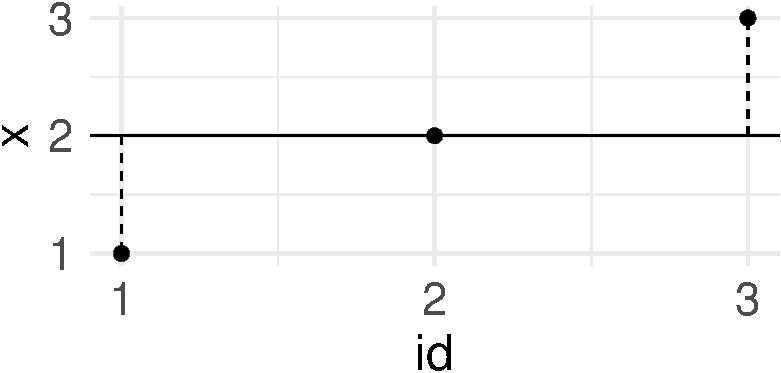
\includegraphics[width=0.5\linewidth,height=\textheight,keepaspectratio]{020-R_files/figure-pdf/fig-vektoriell-1.pdf}

}

\caption{\label{fig-vektoriell}Schema des vektoriellen Rechnens: Eine
Funktion wird auf jedes Element eines Vektors angewandt. Hier:
\(1-2=-1; 2-2=0; 3-2=1\)}

\end{figure}%

\subsection{R-Quiz}\label{r-quiz}

\begin{figure}

\begin{minipage}{0.80\linewidth}
Ihre R-Muskeln sind gestählt? Oder noch nicht so ganz? Macht nichts!
Trainieren Sie sich mit dem R-Quiz auf der
\href{https://sebastiansauer.github.io/Datenwerk/posts/r-quiz/r-quiz}{Datenwerk-Webseite}!
\(\square\)\end{minipage}%
%
\begin{minipage}{0.20\linewidth}

\begin{center}

\includegraphics[width=0.75\linewidth,height=\textheight,keepaspectratio]{020-R_files/figure-pdf/unnamed-chunk-24-1.pdf}
\end{center}

\end{minipage}%

\end{figure}%

\subsection{Ich brauche R-Hilfe!}\label{r-faq}

\begin{itemize}
\tightlist
\item
  \emph{Wo finde ich Hilfe zu einer bestimmten Funktion, z.B.
  \texttt{fun}?} Geben Sie dazu folgenden R-Befehl ein:
  \texttt{help(fun)}. Alternativ geben Sie den Namen der Funktion in
  RStudio im Suchfeld beim Reiter \texttt{Help} ein.
\item
  \emph{Wenn ich ein R-Paket installiere, fragt mich R manchmal, ob ich
  auch Pakete installieren, will, die \enquote{kompiliert} werden
  müssen. Soll ich das machen?} Nein, das ist zumeist nicht nötig; geben
  Sie \enquote{no} ein.
\item
  \emph{In welchem Paket wohnt meine R-Funktion}? Suchen Sie nach der
  Funktion auf der Webseite \emph{RDocumentation}\footnote{\url{https://www.rdocumentation.org/}}.
\item
  \emph{Ich weiß nicht, wie der R-Befehl funktioniert!} Vermutlich haben
  andere Ihr Problem auch, und meistens hat irgendwer das Problem schon
  gelöst. Am besten suchen Sie mal auf
  \textless www.stackoverflow.com\textgreater.
\item
  \emph{Ich muss mal grundlegend verstehen, wozu ein bestimmten R-Paket
  gut ist. Was tun?} Lesen Sie die Dokumenation (\enquote{Vignette})
  eines R-Pakets durch. Für das Paket \texttt{dplyr} bekommen Sie so
  einen Überblick über die verfügbaren Vignetten diese Pakets:
  \texttt{vignette(package\ =\ "dplyr")}. Dann suchen Sie sich aus der
  angezeigten Liste eine Vignette raus; mit \texttt{vignette("rowwise")}
  können Sie sich dann die gewünschte Vignette (z.B. \texttt{rowwise})
  anzeigen lassen.
\item
  \emph{Oh nein, ich seh rot, das heißt, R zeigt mir irgendwas in roter
  Schrift an. Ist jetzt was kaputt?} Keine Sorge, R ist in seiner
  Ausgabe nicht sparsam mit roter Farbe. Solange es nicht als
  Fehlermeldung (\texttt{ERROR}) erscheint, ist es meist kein Problem.
\item
  \emph{R hat sich aufgehängt oder bringt einen Fehler an einer Stelle,
  wo sonst alles funktioniert hat.} Probieren Sie auf jeden Fall mal das
  AEG-Prinzip (Aus-Ein-Gut): sprich, R neu starten.
\item
  \emph{Ich suche schon seit einer Stunde einen Fehler und finde ihn
  nicht. Ich habe schon verschiedene Gegenstände vor Wut an die Wand
  geworfen. Was soll ich tun?} Machen Sie eine Pause. Doch, das ist
  ernst gemeint. Meine Erfahrung: Mit etwas Abstand wird der Kopf klarer
  und man findet das Problem viel einfacher. (Und manchmal ist einem das
  Problem danach schlichtweg egal.)
\item
  \emph{Irgendwie reagiert R komisch, vielleicht hat es sich
  aufgehängt?} Starten Sie R neu. Klicken Sie auf \emph{Session
  \textgreater{} Restart R}.
\item
  \emph{Ich muss mal klar Schiff machen und alle (oder einige) Variablen
  löschen. Wie werd ich das Zeug wieder los?} Beim Neustart von R werden
  alle Objekte (Variablen) gelöscht. Einzelne Objekte können Sie
  selektiv löschen mit dem Befehl \texttt{rm}, so löscht
  \texttt{rm(mariokart)} das Objekt namens \texttt{mariokart}.
\end{itemize}

\begin{tcolorbox}[enhanced jigsaw, leftrule=.75mm, breakable, left=2mm, colback=white, colframe=quarto-callout-caution-color-frame, opacitybacktitle=0.6, coltitle=black, colbacktitle=quarto-callout-caution-color!10!white, arc=.35mm, bottomtitle=1mm, toprule=.15mm, rightrule=.15mm, toptitle=1mm, titlerule=0mm, title=\textcolor{quarto-callout-caution-color}{\faFire}\hspace{0.5em}{Vorsicht}, bottomrule=.15mm, opacityback=0]

R ist penibel: So sind \texttt{name} und \texttt{Name} zwei verschiedene
Variablen für R. \(\square\)

\end{tcolorbox}

Groß- und Kleinschreibung wird von R streng beachtet! Hingegen ist es R
egal, ob Sie zur besseren Übersichtlichkeit Leerzeichen in Ihre Syntax
tippen. Ausnahme sind spezielle Operatoren wie \texttt{\textless{}-}
oder \texttt{\textless{}=}.

Eine gute Nachricht: Wenn R etwas von \texttt{WARNING} (bzw. Warnung)
sagt, können Sie das zumeist ignorieren. Eine \emph{Warnung} ist kein
Fehler (\texttt{ERROR}) und meistens nicht gravierend oder nicht
dringend. Ihre Syntax läuft trotzdem durch. Im Zweifel ist Googeln eine
gute Idee. Nur wenn R von \texttt{Error} spricht, ist es auch ein Fehler
und Ihre Syntax läuft nicht durch.

\section{Mit Daten arbeiten}\label{mit-daten-arbeiten}

\subsection{Wo sind meine Daten?}\label{wo-sind-meine-daten}

Damit Sie eine Datendatei importieren können, müssen Sie wissen, wo die
Datei ist. Schauen wir uns zwei Möglichkeiten an, wo Ihre Datei liegen
könnte.

\begin{enumerate}
\def\labelenumi{\arabic{enumi}.}
\tightlist
\item
  Irgendwo im Internet\footnote{z.B. hier:
    \url{https://vincentarelbundock.github.io/Rdatasets/csv/openintro/mariokart.csv}}
\item
  Irgendwo auf Ihrem Computer, z.B. in Ihrem R-Projektordner
\end{enumerate}

In beiden Fällen wird der \enquote{Aufenthaltsort} der Datei durch den
\emph{Pfad} (Der Pfad einer Datei gibt an, in welchem Ordner und
Unterordner (und Unter-Unterordner) die gesuchte Datei liegt. Ein Pfad
könnte z.B. so aussehen:
\enquote{/Users/sebastiansaueruser/github-repos/statistik1/}.) und den
Namen der Datei definiert.

\begin{tcolorbox}[enhanced jigsaw, leftrule=.75mm, breakable, left=2mm, colback=white, colframe=quarto-callout-note-color-frame, opacitybacktitle=0.6, coltitle=black, colbacktitle=quarto-callout-note-color!10!white, arc=.35mm, bottomtitle=1mm, toprule=.15mm, rightrule=.15mm, toptitle=1mm, titlerule=0mm, title=\textcolor{quarto-callout-note-color}{\faInfo}\hspace{0.5em}{Hinweis}, bottomrule=.15mm, opacityback=0]

Wir werden in diesem Kurs häufiger mit dem Daten \texttt{mariokart}
arbeiten; Sie finden ihn
\href{https://vincentarelbundock.github.io/Rdatasets/csv/openintro/mariokart.csv}{hier}.\footnotemark{}

\end{tcolorbox}

\footnotetext{Auf dieser Webseite
\url{https://vincentarelbundock.github.io/Rdatasets/articles/data.html}
finden Sie eine große Zahl an Datensätzen. Nur für den Fall, dass Ihnen
langweilig ist.}

\subsection{Gebräuchliche
Datenformate}\label{gebruxe4uchliche-datenformate}

Daten werden in verschiedenen Formaten im Computer abgespeichert;
Tabellen häufig als

\begin{itemize}
\tightlist
\item
  Excel-Datei
\item
  CSV-Datei
\end{itemize}

In der Datenanalyse ist das gebräuchlichste Format für Daten in
Tabellenform die \emph{CSV-Datei}. Der Grund ist die technische
Einfachheit dieses Formats.. Für uns Endverbraucher tut das nichts groß
zur Sache, die CSV-Datei beherbergt einfach eine brave Tabelle in einer
\emph{Textdatei}, sonst nichts. In diesem Buch werden wir mit einem
Datensatz namens \texttt{mariokart} arbeiten.

\begin{exercise}[CSV-Datei
öffnen]\protect\hypertarget{exr-csv}{}\label{exr-csv}

~

Öffnen Sie die CSV-Datei \texttt{mariokart.csv} mit einem
\emph{Texteditor} (nicht mit Word und auch nicht mit Excel). Schauen Sie
sich gut an, was Sie dort sehen und erklären Sie die Datenstruktur.

\textbf{Lösung}

Eine CSV-Datei repräsentiert eine Datentabelle. Eine Spaltengrenze wird
mittels eines Kommas dargestellt (man kann auch andere Zeichen wählen,
um Spalten voneinander abzugrenzen).

\end{exercise}

\subsection{Daten importieren}\label{sec-import-mariokart}

Sie können Daten aus verschiedenen Quellen in R importieren: Aus einem
R-Paket, von einer Webseite oder von Ihrem Computer. Dabei ist es egal,
ob Sie die Desktop- oder die Cloud-Version von RStudio nutzen.

Ist Ihr Datensatz schon in einem R-Paket gespeichert, können Sie ihn aus
diesem R-Paket starten. Das ist die bequemste Option. Zum Beispiel
\enquote{wohnt} der Datensatz \texttt{mariokart} im R-Paket
\texttt{openintro}.

\begin{tcolorbox}[enhanced jigsaw, leftrule=.75mm, breakable, left=2mm, colback=white, colframe=quarto-callout-tip-color-frame, opacitybacktitle=0.6, coltitle=black, colbacktitle=quarto-callout-tip-color!10!white, arc=.35mm, bottomtitle=1mm, toprule=.15mm, rightrule=.15mm, toptitle=1mm, titlerule=0mm, title=\textcolor{quarto-callout-tip-color}{\faLightbulb}\hspace{0.5em}{Tipp}, bottomrule=.15mm, opacityback=0]

Häufig wird vergessen, dass ein R-Paket vor der Nutzung installiert
werden muss. \(\square\)

\end{tcolorbox}

Auf der anderen Seite muss man ein R-Paket (wie andere Software auch)
nur \emph{ein} Mal installieren -- das Paket muss man ein Paket
\emph{nach jedem Neustart} von RStudio mit \texttt{library} starten.

\begin{Shaded}
\begin{Highlighting}[]
\FunctionTok{data}\NormalTok{(}\StringTok{"mariokart"}\NormalTok{, }\AttributeTok{package =} \StringTok{"openintro"}\NormalTok{) }\CommentTok{\# Paket muss installiert sein}
\end{Highlighting}
\end{Shaded}

Eine Data-Dictionary findet sich in Anhang~\ref{sec-data-dict}.

Der Befehl \texttt{read.csv} bietet eine Möglichkeit, Daten (in Form
einer Tabelle) von einer Webseite (URL) in R zu importieren, s.
Listing~\ref{lst-mariokart}.

\begin{codelisting}

\caption{\label{lst-mariokart}Mariokart-Datensatz importieren (mit
\texttt{read.csv})}

\centering{

\begin{Shaded}
\begin{Highlighting}[]
\NormalTok{mariokart }\OtherTok{\textless{}{-}} \FunctionTok{read.csv}\NormalTok{(}\FunctionTok{paste0}\NormalTok{(}
  \StringTok{"https://vincentarelbundock.github.io/Rdatasets/"}\NormalTok{,}
  \StringTok{"csv/openintro/mariokart.csv"}\NormalTok{))}
\end{Highlighting}
\end{Shaded}

}

\end{codelisting}%

Es liegt bei Ihnen, welchen Namen Sie der Tabelle geben. Ich persönlich
wähle oft den Namen \texttt{d}, \emph{d} die Daten. \texttt{d} ist ein
kurzer Namen, muss man nicht so viel tippen. Auf der anderen Seite ist
\texttt{d} nicht gerade präzise.

Werfen Sie einen Blick in die Tabelle (engl. \emph{to glimpse}).

\begin{Shaded}
\begin{Highlighting}[]
\FunctionTok{glimpse}\NormalTok{(d)}
\end{Highlighting}
\end{Shaded}

\href{https://vincentarelbundock.github.io/Rdatasets/doc/openintro/mariokart.html}{Online}
findet sich eine Erklärung (Data-Dictionary) des Datensatzes.\footnote{\url{https://vincentarelbundock.github.io/Rdatasets/doc/openintro/mariokart.html}}

Sie können auch von Ihrem Computer aus Daten in RStudio importieren.

Gehen wir davon aus, dass sich die Datendatei im gleichen Ordner wie die
R-Datei (\texttt{.R}- oder \texttt{.qmd}-Datei) befindet, in der Sie den
Befehl zum Importieren schreiben. Dann können Sie die Datei einfach so
importieren:

\begin{Shaded}
\begin{Highlighting}[]
\NormalTok{d }\OtherTok{\textless{}{-}} \FunctionTok{read.csv}\NormalTok{(}\StringTok{"mariokart.csv"}\NormalTok{)}
\end{Highlighting}
\end{Shaded}

\begin{figure}

\begin{minipage}{0.80\linewidth}
\href{https://youtu.be/B_nuN-M0pQM}{Dieses Video} erklärt die Schritte
des Importierens einer Datendatei von Ihrem Computer.\end{minipage}%
%
\begin{minipage}{0.20\linewidth}

\begin{center}

\includegraphics[width=0.75\linewidth,height=\textheight,keepaspectratio]{020-R_files/figure-pdf/unnamed-chunk-30-1.pdf}
\end{center}

\end{minipage}%

\end{figure}%

\subsubsection{Importieren von Ihrem Computer in RStudio
Cloud}\label{importieren-von-ihrem-computer-in-rstudio-cloud}

Das Importieren in von Ihrem Computer zu RStudio Cloud ist identisch zum
Importieren von Ihrem Computer in RStudio Desktop. Nur dass Sie die
Datendatei vorab hochladen müssen, schließlich ist RStudio Cloud in der
Cloud und nicht auf Ihrem Computer. Klicken Sie dazu auf das Icon
\texttt{Upload} im Reiter \texttt{Files}, s.
Abbildung~\ref{fig-upload-to-posit-cloud}. Wählen Sie am besten den
Ordner als Ziel, in dem sich auch die R-Datei, von der aus Sie den
Befehl zum Daten importieren schreiben, befindet.

\begin{figure}

\centering{

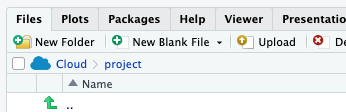
\includegraphics[width=0.5\linewidth,height=\textheight,keepaspectratio]{img/upload-to-posit-cloud.png}

}

\caption{\label{fig-upload-to-posit-cloud}}

\end{figure}%

Es gibt verschiedene Formate, in denen (Tabellen-)Dateien in einem
Computer abgespeichert werden. Die gebräuchlichsten sind CSV und XLSX.
Es gibt auch mehrere R-Befehle, um Daten in R zu importieren, z.B.
\texttt{read.csv} oder \texttt{data\_read}. Praktischerweise kann der
R-Befehl \texttt{data\_read} viele verschiedene Formate automatisch
einlesen, so dass wir uns nicht weiter um das Format kümmern brauchen.
Der Vorteil von \texttt{read.csv} ist, dass Sie kein Extra-Paket
installiert bzw. gestartet haben müssen.

Die GUI (Benutzeroberfläche) von RStudio erlaubt es Ihnen auch, Daten
per Klick, also ohne R-Befehle, zu importieren. Sie können über diese
Maske sowohl CSV-Dateien, Excel-Dateien (XLS, XLSX) oder Daten-Dateien
aus anderen Statistik-Programmen (z.B. SPSS) importieren auf diese
Weise. Zur Erinnerung: CSV-Dateien sind Textdateien, wählen Sie in dem
Fall also \texttt{From\ Text}. Ich empfehle die Variante
\texttt{From\ Text\ (readr)\ ...}.

In der sich öffnenden Maske können Sie unter \texttt{Browse} die zu
importierende Datendatei auswählen. Mit Klick auf \texttt{Import} wird
die Datei schließlich in R importiert.

\subsection{Dataframes}\label{dataframes}

Eine in R importierte Tabelle (mit bestimmten Eigenschaften) heißt
\emph{Dataframe}. Dataframes sind in der Datenanalyse von großer
Bedeutung. Tabelle~\ref{tbl-mariokart} ist die Tabelle mit den
Mariokart-Daten; etwas präziser gesprochen ein Dataframe mit Namen
\texttt{mariokart}. Übrigens ist Tabelle~\ref{tbl-mariokart} in
Normalform (Tidy-Format), vgl. Definition~\ref{def-tidy}.

\begin{definition}[Dataframe]\protect\hypertarget{def-dataframe}{}\label{def-dataframe}

Ein Dataframe (engl. data frame; auch \enquote{Tibble} genannt; von
\enquote{tbl} wie Table) ist ein Datenobjekt in R zur Darstellung von
Tabellen. Dataframes bestehen aus einer oder mehreren Spalten. Spalten
haben einen Namen, sozusagen einen \enquote{Spaltenkopf}. Alle Spalten
müssen die gleiche Länge haben; anschaulich gesprochen ist eine Tabelle
(in R) rechteckig. Jede Spalte einzeln betrachtet kann als Vektor
aufgefasst werden. \(\square\)

\end{definition}

Geben Sie den Namen eines Dataframes ein, um sich den Inhalt anzeigen zu
lassen. Beachten Sie, dass Sie die Daten auf diese Weise nur anschauen,
nicht ändern können.

\subsection{Tabellen in R betrachten}\label{sec-viewtab}

Wenn Sie in R z.B. die Tabelle \texttt{mariokart} in einer
Excel-typischen Ansicht betrachten wollen, klicken Sie am besten auf das
Tabellen-Icon im Reiter \emph{Environment}, gleich neben dem Namen
\texttt{mariokart}, s. Abbildung~\ref{fig-view-mariokart}.

\begin{figure}

\centering{


\includegraphics[width=0.5\linewidth,height=\textheight,keepaspectratio]{img/rstudio-environment-mariokart.png}

}

\caption{\label{fig-view-mariokart}Per Klick auf das Tabellen-Icon
können Sie eine Tabellenansicht der Tabelle \texttt{mariokart} öffnen}

\end{figure}%

Alternativ öffnet der Befehl \texttt{View(mariokart)} die gleiche
Ansicht.

\section{Logikprüfung}\label{sec-logic}

\begin{quote}
{\emoji{student}} Wer will schon wieder wen prüfen?!
\end{quote}

In diesem Abschnitt schauen wir uns \emph{Logikprüfungen} an: Wir lassen
R prüfen, ob eine Variable einen bestimmten Wert hat oder größer/kleiner
als ein Referenzwert ist.

Definieren wir zuerst eine Variable, \texttt{x}.

\begin{Shaded}
\begin{Highlighting}[]
\NormalTok{x }\OtherTok{\textless{}{-}} \DecValTok{42}
\end{Highlighting}
\end{Shaded}

Dann fragen wir R, ob diese Variable den Wert \texttt{42} hat.

\begin{Shaded}
\begin{Highlighting}[]
\NormalTok{x }\SpecialCharTok{==} \DecValTok{42}
\DocumentationTok{\#\# [1] TRUE}
\end{Highlighting}
\end{Shaded}

\begin{quote}
{\emoji{robot}} Hallo, Mensch. Ja, diese Variable hat den Wert 42.
\end{quote}

(Danke, R.)

Möchte man mit R prüfen, ob eine Variable \texttt{x} einen bestimmten
\texttt{Wert} (\enquote{Inhalt}) hat, so schreibt man:

\texttt{x\ ==\ Wert}.

Man beachte das \emph{doppelte} Gleichheitszeichen. Zur Prüfung auf
Gleichheit muss man das doppelte Gleichheitszeichen verwenden.

\begin{tcolorbox}[enhanced jigsaw, leftrule=.75mm, breakable, left=2mm, colback=white, colframe=quarto-callout-caution-color-frame, opacitybacktitle=0.6, coltitle=black, colbacktitle=quarto-callout-caution-color!10!white, arc=.35mm, bottomtitle=1mm, toprule=.15mm, rightrule=.15mm, toptitle=1mm, titlerule=0mm, title=\textcolor{quarto-callout-caution-color}{\faFire}\hspace{0.5em}{Vorsicht}, bottomrule=.15mm, opacityback=0]

Ein beliebter Fehler ist es, bei der Prüfung auf Gleichheit, nur ein
Gleichheitszeichen zu verwenden, z.B. so: \texttt{x\ =\ 73}. Mit einem
Gleichheitszeichen prüft man aber \emph{nicht} auf Gleichheit, sondern
man definiert die Variable oder bestimmt ein Funktionsargument, s.
Kapitel~\ref{sec-rvars}. \(\square\)

\end{tcolorbox}

Tabelle~\ref{tbl-lgl} gibt einen Überblick über wichtige Logikprüfungen
in R. (Um das Zeichen für das logische ODER, \texttt{\textbar{}} auf
einer Mac-Tastatur zu erhalten, drückt man \emph{Option+7}.)

\begin{longtable}[]{@{}ll@{}}

\caption{\label{tbl-lgl}Logische Prüfungen in R}

\tabularnewline

\toprule\noalign{}
Prüfung.auf & R-Syntax \\
\midrule\noalign{}
\endhead
\bottomrule\noalign{}
\endlastfoot
Gleichheit & x == Wert \\
Ungleichheit & x != Wert \\
Größer als Wert & x \textgreater{} Wert \\
Größer oder gleich Wert & x \textgreater= Wert \\
Kleiner als Wert & x \textless{} Wert \\
Kleiner oder gleich Wert & x \textless= Wert \\
Logisches UND & (x \textless{} Wert1) \& (x \textgreater{} Wert2) \\
Logisches ODER & (x \textless{} Wert1) \textbar{} (x \textgreater{}
Wert2) \\

\end{longtable}

\section{Praxisbezug}\label{praxisbezug-1}

\begin{quote}
{\emoji{student}} R in der Praxis wirklich genutzt? Oder ist R nur der
Traum von (vielleicht verwirrten) Profs im Elfenbeinturm?
\end{quote}

Schauen wir uns dazu die Suchanfragen bei
\href{www.stackoverflow.com}{stackoverflow.com} an, dem größten
FAQ-Forum für Software-Entwicklung. Wir vergleichen Suchanfragen mit dem
Tag \texttt{{[}r{]}} zu Suchanfragen mit dem Tag
\texttt{{[}spss{]}}(SPSS ist eine an Hochschulen verbreitete
Statistik-Software). Die Ergebnisse sind in Abbildung
Abbildung~\ref{fig-stackoverflow1} dargestellt\footnote{Die Daten wurden
  am 2022-02-24, 17:21 CET, abgerufen.}

\begin{figure}

\centering{

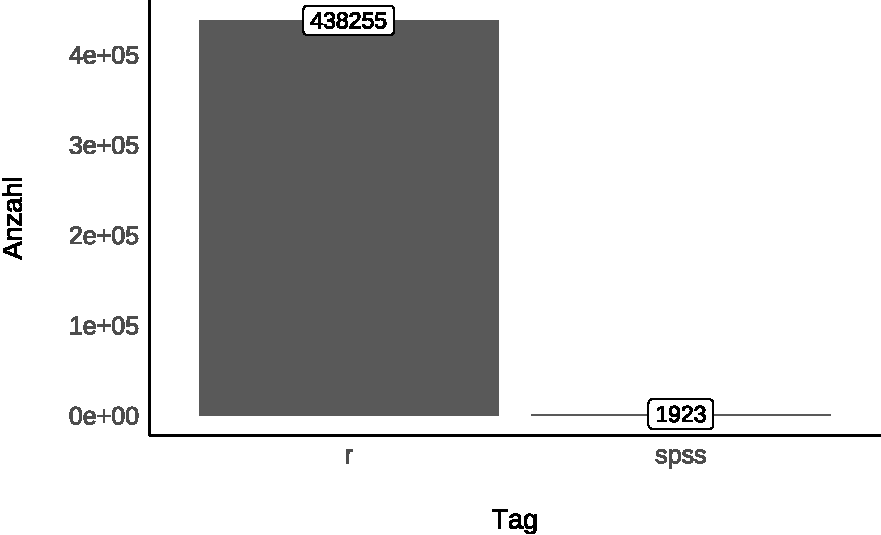
\includegraphics[width=0.75\linewidth,height=\textheight,keepaspectratio]{020-R_files/figure-pdf/fig-stackoverflow1-1.pdf}

}

\caption{\label{fig-stackoverflow1}Suchanfragen nach R bzw SPSS, Stand
2022-02-24}

\end{figure}%

Das ist grob gerechnet ein Faktor von 200 (der Unterschied von R zu
SPSS). Dieses Ergebnis lässt darauf schließen, dass R in der Praxis viel
mehr als SPSS gebraucht wird.

\begin{quote}
{\emoji{student}} Aber ist R wirklich ein Werkzeug, das mir im Job
hilft?
\end{quote}

\begin{quote}
{\emoji{teacher}} Viele Firmen weltweit nutzen R zur
Datenanalyse.\footnote{wie diese Liste zeigt:
  \url{https://www.quora.com/Which-organizations-use-R?share=1} zeigt}.
\end{quote}

\begin{quote}
{\emoji{woman-student}} R ist \emph{der} Place-to-be für die
Datenanalyse.
\end{quote}

\begin{quote}
{\emoji{student}} Aber ist Datenanalyse wirklich etwas, womit ich in
Zukunft einen guten Job bekomme?
\end{quote}

\begin{quote}
{\emoji{teacher}} Berufe mit Bezug zu Daten, Datenanalyse oder,
allgemeiner, Künstlicher Intelligenz (artificial intelligence) gehören
zu den stark wachsenden Berufen:
\end{quote}

\begin{quote}
Artificial intelligence (AI) continues to make a strong showing on our
Emerging Jobs lists, which is no surprise. Many jobs that have risen up
as a result of AI in fields like cybersecurity and data science and
because it's is so pervasive many roles may demand more knowledge of AI
than you may think. For example, real estate and business development
roles (Berger, 2019).
\end{quote}

\section{Aufgaben}\label{aufgaben-1}

\begin{exercise}[Statistik-Meme]\protect\hypertarget{exr-meme}{}\label{exr-meme}

Suchen Sie ein schönes Meme zum Thema Statistik, Datenanalyse und Data
Science. \(\square\)

\end{exercise}

Die Webseite \href{https://datenwerk.netlify.app}{datenwerk.netlify.app}
stellt eine Reihe von einschlägigen Übungsaufgaben bereit. Sie können
die Suchfunktion der Webseite nutzen, um die Aufgaben mit den folgenden
Namen zu suchen:

\begin{enumerate}
\def\labelenumi{\arabic{enumi}.}
\tightlist
\item
  \href{https://sebastiansauer.github.io/Datenwerk/posts/typ-fehler-r-01/typ-fehler-r-01.html}{Typ-Fehler-R-01}
\item
  \href{https://sebastiansauer.github.io/Datenwerk/posts/typ-fehler-r-02/typ-fehler-r-02.html}{Typ-Fehler-R-02}
\item
  \href{https://sebastiansauer.github.io/Datenwerk/posts/typ-fehler-r-03/typ-fehler-r-03.html}{Typ-Fehler-R-03}
\item
  \href{https://sebastiansauer.github.io/Datenwerk/posts/typ-fehler-r-04/typ-fehler-r-04.html}{Typ-Fehler-R-04}
\item
  \href{https://sebastiansauer.github.io/Datenwerk/posts/typ-fehler-r-06a/typ-fehler-r-06a.html}{Typ-Fehler-R-06a}
\item
  \href{https://sebastiansauer.github.io/Datenwerk/posts/typ-fehler-r-07/typ-fehler-r-07.html}{Typ-Fehler-R-07}
\item
  \href{https://sebastiansauer.github.io/Datenwerk/posts/typ-fehler-r-08-name-clash/typ-fehler-r-08-name-clash}{Typ-Fehler-R-08-name-clash}
\item
  \href{https://sebastiansauer.github.io/Datenwerk/posts/logikpruefung1/logikpruefung1}{Logikpruefung1}
\item
  \href{https://sebastiansauer.github.io/Datenwerk/posts/logikpruefung2/logikpruefung2}{Logikpruefung2}
\item
  \href{https://sebastiansauer.github.io/Datenwerk/posts/there-is-no-package/there-is-no-package.html}{there-is-no-package}
\item
  \href{https://sebastiansauer.github.io/Datenwerk/posts/wertberechnen2/wertberechnen2}{Wertberechnen2}
\item
  \href{https://sebastiansauer.github.io/Datenwerk/posts/wertzuweisen_mc/wertzuweisen_mc}{Wertzuweisen\_mc}
\item
  \href{https://sebastiansauer.github.io/Datenwerk/posts/argumente/argumente.html}{argumente}
\item
  \href{https://sebastiansauer.github.io/Datenwerk/posts/import-mtcars/import-mtcars.html}{import-mtcars}
\item
  \href{https://sebastiansauer.github.io/Datenwerk/posts/wertzuweisen/wertzuweisen}{Wertzuweisen}
\item
  \href{https://sebastiansauer.github.io/Datenwerk/posts/wertpruefen/wertpruefen}{Wertpruefen}
\item
  \href{https://sebastiansauer.github.io/Datenwerk/posts/wrangle1/wrangle1.html}{wrangle1}
\item
  \href{https://sebastiansauer.github.io/Datenwerk/posts/repro1-sessioninfo/repro1-sessioninfo.html}{repro1-sessioninfo}
\item
  \href{https://sebastiansauer.github.io/Datenwerk/posts/mw-berechnen/mw-berechnen}{mw-berechnen}
\end{enumerate}

Prüfen Sie Ihr Wissen zu R mit
\href{https://sebastiansauer.github.io/Datenwerk/posts/r-quiz/r-quiz}{einem
Quiz}!\footnote{\url{https://sebastiansauer.github.io/Datenwerk/posts/r-quiz/r-quiz}}
Noch nicht genug? Checken Sie alle Aufgaben mit dem Tag
\href{https://sebastiansauer.github.io/Datenwerk/\#category=R}{R} auf
dem Datenwerk aus.\footnote{\url{https://sebastiansauer.github.io/Datenwerk/\#category=R}}

\begin{tcolorbox}[enhanced jigsaw, leftrule=.75mm, breakable, left=2mm, colback=white, colframe=quarto-callout-note-color-frame, opacitybacktitle=0.6, coltitle=black, colbacktitle=quarto-callout-note-color!10!white, arc=.35mm, bottomtitle=1mm, toprule=.15mm, rightrule=.15mm, toptitle=1mm, titlerule=0mm, title=\textcolor{quarto-callout-note-color}{\faInfo}\hspace{0.5em}{Hinweis}, bottomrule=.15mm, opacityback=0]

Die Webseite
\href{https://sebastiansauer.github.io/Datenwerk/}{Datenwerk} stellt
eine Reihe von Aufgaben zum Thema Statistik bereit. \(\square\)

\end{tcolorbox}

Jeder Aufgabe sind im Datenwerk ein oder mehrere Schlagwörter (Tags)
zugeordnet. Wenn Sie auf ein Schlagwort klicken, sehen Sie die Liste der
Aufgaben mit diesem Schlagwort. Es kann aber sein, dass Sie einige
Aufgabe nicht lösen können, da Wissen vorausgesetzt wird, das Sie (noch)
nicht haben. Lassen Sie sich davon nicht ins Boxhorn jagen. Ignorieren
Sie solche Aufgaben fürs Erste.

\section{Vertiefung}\label{vertiefung-2}

\subsection{\texorpdfstring{Alternativen zu
\texttt{read.csv}}{Alternativen zu read.csv}}\label{alternativen-zu-read.csv}

Eine weitere Möglichkeit, um Daten von einem Ordner (egal ob dieser sich
im Internet oder auf Ihrem Computer befindet) einzulesen, stellt die
Funktion \texttt{data\_read} bereit:

\begin{Shaded}
\begin{Highlighting}[]
\FunctionTok{library}\NormalTok{(easystats)  }\CommentTok{\# Das Paket muss installiert sein}
\NormalTok{d }\OtherTok{\textless{}{-}} \FunctionTok{data\_read}\NormalTok{(}\FunctionTok{paste0}\NormalTok{(}
  \StringTok{"https://vincentarelbundock.github.io/Rdatasets/"}\NormalTok{,}
  \StringTok{"csv/openintro/mariokart.csv"}\NormalTok{))}
\end{Highlighting}
\end{Shaded}

Der Unterschied ist, dass \texttt{data\_read} eine Vielzahl an Formaten
von Daten (XLSX, CSV, SPSS, \ldots) verkraftet, wohingegen
\texttt{read.csv} nur Standard-CSV einlesen kann.

Schauen wir uns die letzte R-Syntax im Detail an:

\begin{verbatim}
Hey R,
hol das "Buch" easystats aus der Bücherei und lies es
definiere als "d" die Tabelle,
die du unter der angegebenen URL findest.
\end{verbatim}

In R gibt es oft viele Möglichkeiten, ein Ziel zu erreichen. Zum
Beispiel haben wir hier den Befehl \texttt{data\_read} verwendet, um
Daten zu importieren. Andere, gebräuchliche Befehle, die CSV-Dateien
importieren, heißen \texttt{read.csv} (aus dem Standard-R, kein
Extra-Paket nötig) und \texttt{read\_csv} (aus dem Meta-Paket
\texttt{tidyverse}).

\subsection{Importieren von
Excel-Tabellen}\label{importieren-von-excel-tabellen}

Mit der Funktion \texttt{data\_read} aus \texttt{\{easystats\}} kann man
viele verschiedene Datenformate importieren, auch Excel-Tabellen (.xls,
.xlsx).

Als Beispiel betrachten wir den Datensatz \texttt{extra} aus dem R-Paket
\texttt{\{pradadata\}}\footnote{\url{https://github.com/sebastiansauer/pradadata}}.
In diesem Datensatz werden die Ergebnisse einer Umfrage zu den
Korrelaten von Extraversion beschrieben. Details zu der zugrunde
liegenden Studie finden Sie hier: \url{https://osf.io/4kgzh}.\footnote{Ein
  Daten-Dictionary findet sich hier:
  \url{https://github.com/sebastiansauer/statistik1/raw/main/data/extra-dictionary.md}.}
Laden Sie die Excel-Datei herunter. Angenommen, Sie speichern die
Excel-Datei in einem Unterordner namens \texttt{daten} Ihres aktuellen
Projektordners. Dann können Sie die Daten so importieren:

\begin{Shaded}
\begin{Highlighting}[]
\FunctionTok{library}\NormalTok{(easystats)}
\NormalTok{extra }\OtherTok{\textless{}{-}} \FunctionTok{data\_read}\NormalTok{(}\StringTok{"data/extra.xls"}\NormalTok{)}
\end{Highlighting}
\end{Shaded}

Allerdings kann \texttt{data\_read} keine Dateien aus dem Internet
importieren, was praktisch wäre. Stattdessen muss die Datei lokal auf
Ihrer Festplatte liegen.

Wenn Sie allerdings \enquote{remote}, also aus dem Internet, eine
Excel-Datei importieren möchten, so können Sie das mit \texttt{import}
aus dem R-Paket \texttt{\{rio\}} tun:

\begin{Shaded}
\begin{Highlighting}[]
\FunctionTok{library}\NormalTok{(rio)}
\NormalTok{extra\_path }\OtherTok{\textless{}{-}} \FunctionTok{paste0}\NormalTok{(}
  \StringTok{"https://github.com/sebastiansauer/statistik1/"}\NormalTok{,}
  \StringTok{"raw/main/data/extra.xls"}\NormalTok{)}
\NormalTok{extra }\OtherTok{\textless{}{-}} \FunctionTok{import}\NormalTok{(extra\_path)}
\end{Highlighting}
\end{Shaded}

CSV-Dateien werden auf vielen Computern als eine Datei erkannt, die
Excel öffnen kann und das auch tut, wenn man eine CSV-Datei
doppelklickt. Dennoch ist das CSV-Format keine Datei im Excel-Format,
sondern eine einfache Text-Datei, die auch mit jedem Text-Editor
geöffnet und bearbeitet werden kann. Alternativ können Sie in RStudio
auch Excel-Dateien \emph{ohne} R-Code importieren.

\subsection{Der Dollar-Operator}\label{sec-dollar-op}

In Definition~\ref{def-veccalc} hatten wir Vektoren definiert. Solche
Vektoren fliegen sozusagen frei in Ihrem \texttt{Environment} herum
(Schauen Sie mal dort nach!) Die Spalten einer Tabelle sind aber auch
Vektoren, nur eben nicht frei im \texttt{Environment}, sondern in eine
Tabelle eingebunden. Möchte man diese Vektoren direkt ansprechen, so
kann man das mit dem sog. \emph{Dollar-Operator} \texttt{\$} tun.
Angenommen, Sie möchten sich die Verkaufspreise (\texttt{total\_pr}) aus
der Tabelle \texttt{mariokart} herausziehen, dann können Sie das mit dem
Dollar-Operator tun:

\begin{Shaded}
\begin{Highlighting}[]
\NormalTok{mariokart}\SpecialCharTok{$}\NormalTok{total\_pr }\SpecialCharTok{|\textgreater{}} \FunctionTok{head}\NormalTok{()}
\DocumentationTok{\#\# [1] 52 37 46 44 71 45}
\end{Highlighting}
\end{Shaded}

Der Dollar-Operator trennt den Namen der Tabelle vom Namen der Spalte.

Natürlich können Sie mit dem resultierenden Vektor beliebig
weiterarbeiten, etwa ihn in einem anderen Vektor speichern oder eine
Funktion anwenden:

\begin{Shaded}
\begin{Highlighting}[]
\NormalTok{verkaufspreise }\OtherTok{\textless{}{-}}\NormalTok{ mariokart}\SpecialCharTok{$}\NormalTok{total\_pr}
\FunctionTok{mean}\NormalTok{(verkaufspreise)}
\FunctionTok{mean}\NormalTok{(mariokart}\SpecialCharTok{$}\NormalTok{total\_pr)  }\CommentTok{\# synonym zur obigen Zeile}
\DocumentationTok{\#\# [1] 50}
\DocumentationTok{\#\# [1] 50}
\end{Highlighting}
\end{Shaded}

\subsection{R-Funktionen
verschachteln}\label{r-funktionen-verschachteln}

Das Kombinieren von Funktionen kann kompliziert werden:

\begin{codelisting}

\caption{\label{lst-schachtel}Verschachtelte Funktionen}

\centering{

\begin{Shaded}
\begin{Highlighting}[]
\NormalTok{x }\OtherTok{\textless{}{-}} \FunctionTok{c}\NormalTok{(}\DecValTok{1}\NormalTok{, }\DecValTok{2}\NormalTok{, }\DecValTok{3}\NormalTok{)}
\FunctionTok{sum}\NormalTok{(}\FunctionTok{abs}\NormalTok{(}\FunctionTok{mean}\NormalTok{(x)}\SpecialCharTok{{-}}\NormalTok{x)) }
\DocumentationTok{\#\# [1] 2}
\end{Highlighting}
\end{Shaded}

}

\end{codelisting}%

Die Funktion \texttt{abs(x)} gibt den (Absolut-)Betrag von \texttt{x}
zurück (entfernt das Vorzeichen).

Verschachtelte Ausdrücke lesen sich von innen nach außen (und werden in
dieser Reihenfolge abgearbeitet). Für unser Beispiel
(Listing~\ref{lst-schachtel}):

\begin{enumerate}
\def\labelenumi{\arabic{enumi}.}
\tightlist
\item
  Berechne den Mittelwert von \texttt{x}
\item
  Ziehe vom Mittelwert jeweils die Elemente von \texttt{x} ab
\item
  Nimm vom Ergebnis jeweils den Absolutwert
\item
  Summiere diese Werte
\end{enumerate}

Kurz gesagt: Hier haben wir die mittlere Absolutabweichung der Elemente
von \texttt{x} zum Mittelwert ausgerechnet.

\subsection{R und Friends updaten}\label{r-und-friends-updaten}

Irgendwann werden wir mit unsere Version von R und RStudio veraltet
sein. Installieren Sie dann einfach die neue Version von R und RStudio
wie oben beschrieben, s. Kapitel~\ref{sec-install-r}.

So updaten Sie Ihre R-Pakete: Klicken Sie im Reiter \texttt{Packages}
(in RStudio) auf \texttt{Update}. Wenn die Anzahl der zu
aktualisierenden Pakete groß ist, dann besser nicht alle auswählen,
sondern nur ein paar. Dann die nächsten paar Pakete usw. Denken Sie
daran, dass Sie die Software (R, RStudio, R-Paket), die Sie
updaten/installieren, nicht ausgefüht werden darf.

\subsection{Benötigte Daten}\label{benuxf6tigte-daten-1}

Sie benötigen in diesem Kapitel den Datensatz \texttt{mariokart}, der
entweder online\footnote{ über diese Internetadresse:
  \url{https://vincentarelbundock.github.io/Rdatasets/csv/openintro/mariokart.csv}}
oder über R-Paket \texttt{openintro} importiert werden kann.

Import via Download:

\begin{Shaded}
\begin{Highlighting}[]
\NormalTok{mariokart }\OtherTok{\textless{}{-}} \FunctionTok{read.csv}\NormalTok{(}\FunctionTok{paste0}\NormalTok{(}
  \StringTok{"https://vincentarelbundock.github.io/Rdatasets/"}\NormalTok{,}
  \StringTok{"csv/openintro/mariokart.csv"}\NormalTok{))}
\end{Highlighting}
\end{Shaded}

Import via R-Paket:

\begin{Shaded}
\begin{Highlighting}[]
\CommentTok{\# Das Paket \textquotesingle{}openintro\textquotesingle{} muss installiert sein:}
\FunctionTok{data}\NormalTok{(mariokart, }\AttributeTok{package =} \StringTok{"openintro"}\NormalTok{) }
\end{Highlighting}
\end{Shaded}

\section{Literaturhinweise}\label{literaturhinweise-1}

\enquote{Warum R? Warum, R?} heißt ein Kapitel in Sauer (2019), das
einiges zum Pro und Contra von R ausführt. Kapitel 3 in derselben Quelle
enthält Hinweise zum Starten von R. Kapitel 4 erläutert die Grundlagen
von \enquote{Errisch}. Kapitel 5 führt in die Datenstrukturen von R ein
(etwas anspruchsvoller). Alternativ bietet
\href{https://moderndive.com/1-getting-started.html}{Kapitel 1} von
Ismay \& Kim (2020) einen guten und anwenderfreundlichen Überblick. Das
Buch hat auch den Vorteil, dass es komplett frei online verfügbar ist.
Vergleichbar dazu ist Cetinkaya-Rundel \& Hardin (2021), vielleicht
einen Tick formaler; auf jeden Fall genau das richtige Niveau für
Bachelor-Statistik in angewandten nicht-technischen Studiengängen.

\chapter{Daten umformen}\label{daten-umformen}

\[
\definecolor{ycol}{RGB}{230,159,0}
\definecolor{modelcol}{RGB}{86,180,233}
\definecolor{errorcol}{RGB}{0,158,115}
\definecolor{beta0col}{RGB}{213,94,0}
\definecolor{beta1col}{RGB}{0,114,178}
\definecolor{xcol}{RGB}{204,121,167}
\]

\section{Einstieg}\label{einstieg-3}

\subsection{Lernziele}\label{lernziele-3}

\begin{itemize}
\tightlist
\item
  Sie können folgende Verben des Datenjudo anwenden: \texttt{arrange},
  \texttt{filter}, \texttt{select}, \texttt{summarise},
  \texttt{group\_by}, \texttt{mutate}.
\item
  Sie können R-Befehle mit der \enquote{Pfeife} verketten.
\end{itemize}

\begin{exercise}[Mariokart
importieren]\protect\hypertarget{exr-los}{}\label{exr-los}

Importieren Sie den Datensatz \texttt{mariokart}, s
Kapitel~\ref{sec-import-mariokart}. Probieren Sie alle vorgestellten
Verben des Datenjudos aus, zunächst, indem Sie einfach den R-Code
kopieren und selber ausführen. \(\square\)

\end{exercise}

\subsection{Frag den Bot}\label{frag-den-bot}

\begin{quote}
{\emoji{student}} Erkläre einem Fünfjährigen, warum Statistik nützlich
ist.
\end{quote}

\begin{quote}
{\emoji{robot}} Okay, hör zu. Stell dir vor, du hast viele
Spielzeugautos und du willst herausfinden, welches Auto am meisten
bespielt wird. Du kannst jeden Tag zählen, wie oft du jedes Auto benutzt
hast. Aber das wäre sehr mühsam und könnte schnell durcheinander
gebracht werden. Stattdessen kannst du mit Statistik eine einfachere
Methode finden. Du kannst zum Beispiel eine Liste machen und jedes Auto
mit einer bestimmten Farbe markieren. Dann kannst du jeden Tag einfach
zählen, wie oft du jede Farbe verwendet hast. Am Ende kannst du
herausfinden, welches Auto am meisten bespielt wurde, indem du siehst,
welche Farbe am meisten verwendet wurde. Das ist ein Beispiel dafür, wie
Statistik uns dabei helfen kann, Muster in großen Datensätzen zu finden
und Entscheidungen zu treffen, ohne alles einzeln zu zählen.\footnote{Quelle:
  ChatGTP 3.5, 2023-02-09}
\end{quote}

\begin{definition}[Datenjudo]\protect\hypertarget{def-datenjudo}{}\label{def-datenjudo}

Mit \emph{Datenjudo} meint man den Prozess der Aufbereitens, Umformens
oder Zusammenfassen von Daten, sowohl für einzelne Beobachtungen (Zeilen
einer Datentabelle) oder Variablen (Spalten einer Datentabelle) oder
einer ganzen Datentabelle. \(\square\)

\end{definition}

\subsection{Praxisbezug: Aus dem Alltag des Data
Scientisten}\label{praxisbezug-aus-dem-alltag-des-data-scientisten}

Denkt man an Data Science, stellt man sich coole Leute vor (in San
Francisco oder Berlin), die an abgefahrenen Berechnungen mit hoch
komplexen statistischen Modellen für gigantische Datenmengen basteln.
Laut dem \emph{Harvard Business Review} allerdings, verbringen Data
Scientisten \enquote{80\%} ihrer Zeit mit dem \emph{Aufbereiten} von
Daten (Bowne-Anderson, 2018). Ja: mit uncoolen Tätigkeiten wie
Tippfehler aus Datensätzen entfernen oder die Daten überhaupt nutzbar
und verständlich zu machen.

Das zeigt zumindest, dass das Aufbereiten von Daten a) wichtig ist und
b) dass man allein damit schon weit kommen kann. Eine gute Nachricht ist
(vielleicht), dass das Aufbereiten von Daten keine aufwändige Mathematik
verlangt, stattdessen muss man ein paar Handgriffe und Kniffe kennen.
Daher passt der Begriff \emph{Datenjudo} vielleicht ganz gut. Kümmern
wir uns also um das Aufbereiten bzw. Umformen von Daten, um das
Datenjudo. \(\square\)

\begin{example}[Beispiel für
Datenjudo]\protect\hypertarget{exm-datenjudo}{}\label{exm-datenjudo}

Beispiele für typische Tätigkeiten des Datenjudos sind:

\begin{itemize}
\tightlist
\item
  Zeilen \emph{filtern} (z.B. nur Studentis des Studiengangs X)
\item
  Zeilen \emph{sortieren} (z.B. Studenten mit guten Noten in den oberen
  Zeilen)
\item
  Spalten \emph{wählen} (z.B. 100 weitere Produkte ausblenden)
\item
  Spalten in eine Zahl \emph{zusammenfassen} (z. B. Notenschnitt der 1.
  Klausur)
\item
  Tabelle \emph{gruppieren} (z.B. Analyse getrennt nach Standorten)
\item
  Werte aus einer Spalte \emph{verändern} oder \emph{neue Spalte} bilden
  (z. B. Punkte in Prozent-Richtige umrechnen).
\item
  \ldots{} \(\square\)
\end{itemize}

\end{example}

\subsection{Mach's einfach}\label{machs-einfach}

Es gibt einen (einfachen) Trick, wie man umfangreiche Datenaufbereitung
elegant geregelt kriegt.

Der Trick besteht darin, komplexe Operationen in mehrere einfache
Teilschritte zu zergliedern. (In gewisser Weise besteht das Wesen einer
Analyse eben darin: die Zerlegung eines Gegenstands in seine
Bestandteile.) Man könnte vom \enquote{Lego-Prinzip} sprechen, s.
Abbildung~\ref{fig-lego}. Im linken Teil von Abbildung~\ref{fig-lego}
sieht man ein (recht) komplexes Gebilde. Zerlegt man es aber in seine
Einzelteile, so sind es deutlich einfachere geometrische Objekte wie
Dreiecke oder Quadrate (rechter Teil des Diagramms). Damit Sie es selber
einfach machen können, müssen Sie selber Hand anlegen. Importieren Sie
daher den Datensatz \texttt{mariokart}, s.
Kapitel~\ref{sec-import-mariokart}.

\begin{figure}

\centering{


\includegraphics[width=0.75\linewidth,height=\textheight,keepaspectratio]{img/Bausteine_dplyr_crop.pdf}

}

\caption{\label{fig-lego}Das Lego-Prinzip (Sauer, 2019)}

\end{figure}%

\begin{example}[Der Datenguru in
Aktion]\protect\hypertarget{exm-datenjudo}{}\label{exm-datenjudo}

Sie arbeiten immer noch bei dem großen Online-Auktionshaus. Mittlerweile
haben Sie sich den Ruf des \enquote{Datenguru} erworben. Vielleicht,
weil Sie behauptet haben, Data Science sei zu 80\% Datenjudo, das hat
irgendwie Eindruck geschindet\ldots{} Naja, jedenfalls müssen Sie jetzt
mal zeigen, dass Sie nicht nur schlaue Sprüche draufhaben, sondern auch
die Daten ordentlich abbürsten können. Sie analysieren dafür im
Folgenden den Datensatz \texttt{mariokart}. Na, dann los. \(\square\)

\end{example}

\section{Die Verben des Datenjudos}\label{die-verben-des-datenjudos}

Im R-Paket \texttt{dplyr}, das wiederum Teil des R-Pakets
\texttt{tidyverse} ist, gibt es eine Reihe von R-Befehlen, die das
Datenjudo in eine Handvoll einfacher Verben herunterbrechen. (Falls Sie
das R-Paket \texttt{tidyverse} noch nicht installiert haben sollten,
wäre jetzt ein guter Zeitpunkt dafür.) Die wichtigsten Verben des
Datenjudos schauen wir uns im Folgenden an.

Wir betrachten dazu im Folgenden einen einfachen (Spielzeug-)Datensatz,
an dem wir zunächst die Verben des Datenjudos vorstellen, s.
Tabelle~\ref{tbl-datenjudo}.

\begin{longtable}[]{@{}rllr@{}}

\caption{\label{tbl-datenjudo}Ein einfacher Datensatz von schlichtem
Gemüt}

\tabularnewline

\toprule\noalign{}
id & name & gruppe & note \\
\midrule\noalign{}
\endhead
\bottomrule\noalign{}
\endlastfoot
1 & Anni & A & 2.7 \\
2 & Berti & A & 2.7 \\
3 & Charli & B & 1.7 \\

\end{longtable}

Die Verben des Datenjudos wohnen im Paket \texttt{dplyr}, welches
gestartet wird, wenn Sie \texttt{library(tidyverse)} eingeben. Falls Sie
vergessen , das Paket \texttt{tidyverse} zu starten, dann funktionieren
diese Befehle nicht.

\subsection{\texorpdfstring{Tabelle sortieren:
\texttt{arrange}}{Tabelle sortieren: arrange}}\label{tabelle-sortieren-arrange}

\emph{Sortieren} der Zeilen ist eine einfache, aber häufige Tätigkeit
des Datenjudos, s. Abbildung~\ref{fig-arrange}.

\begin{figure}

\centering{

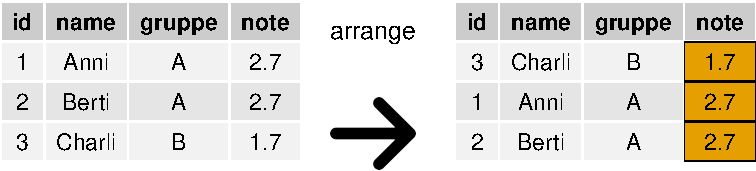
\includegraphics[width=1\linewidth,height=\textheight,keepaspectratio]{030-aufbereiten_files/figure-pdf/fig-arrange-1.pdf}

}

\caption{\label{fig-arrange}Sinnbild für das Sortieren einer Tabelle mit
\texttt{arrange}}

\end{figure}%

\begin{example}[Was sind die höchsten
Preise?]\protect\hypertarget{exm-arrange1}{}\label{exm-arrange1}

Sie wollen mal locker anfangen. Daher stellen Sie sich folgende Frage:
Was sind denn eigentlich die höchsten Preise, für die das Spiel
\emph{Mariokart} über den Online-Ladentisch geht? Die Spalte für den
Verkaufsprei heißt offenbar \texttt{total\_pr} (s. Datensatz
\texttt{mariokart}). In Excel kann die Spalte, nach der man die Tabelle
sortieren möchte, einfach anklicken. Ob das in R auch so einfach geht?

Die Funktion \texttt{arrange} macht es uns ziemlich einfach, s.
tbl-arrange-pdf.

\begin{Shaded}
\begin{Highlighting}[]
\FunctionTok{arrange}\NormalTok{(mariokart, total\_pr) }
\end{Highlighting}
\end{Shaded}

\begin{longtable}[]{@{}rr@{}}

\caption{\label{tbl-arrange-pdf}Die Datentabelle, sortiert nach
\texttt{total\_pr}}

\tabularnewline

\toprule\noalign{}
total\_pr & start\_pr \\
\midrule\noalign{}
\endhead
\bottomrule\noalign{}
\endlastfoot
29 & 0.99 \\
30 & 0.01 \\
31 & 0.99 \\
31 & 1.99 \\
31 & 30.00 \\
31 & 0.01 \\

\end{longtable}

Übersetzen wir die R-Syntax ins Deutsche:

\begin{verbatim}
Hey R,
arrangiere (sortiere) `mariokart` nach der Spalte `total_pr` (aufsteigend).
\end{verbatim}

Gar nicht so schwer. \(\square\)

\end{example}

Übrigens wird in \texttt{arrange} per Voreinstellung aufsteigend
sortiert. Setzt man ein Minus vor der zu sortierenden Spalte, wird
umgekehrt, also \emph{absteigend} sortiert:

\begin{Shaded}
\begin{Highlighting}[]
\NormalTok{mario\_sortiert }\OtherTok{\textless{}{-}} \FunctionTok{arrange}\NormalTok{(mariokart, }\SpecialCharTok{{-}}\NormalTok{total\_pr)}
\end{Highlighting}
\end{Shaded}

\begin{exercise}[]\protect\hypertarget{exr-arrange2}{}\label{exr-arrange2}

Sortieren Sie die Mariokart-Daten absteigend nach der Anzahl der
beigelegten Lenkräder. \(\square\)

\end{exercise}

\subsection{\texorpdfstring{Zeilen filtern:
\texttt{filter}}{Zeilen filtern: filter}}\label{zeilen-filtern-filter}

Zeilen \emph{filtern} bedeutet, dass man nur \emph{bestimmte}
\emph{Zeilen} (Beobachtungen) \emph{behalten} möchte, die restlichen
Zeilen brauchen wir nicht, weg mit ihnen. Wir haben also ein
Filterkriterium im Kopf, anhand dessen wir die Tabelle filern, s.
Abbildung~\ref{fig-filter}.

\begin{figure}

\centering{

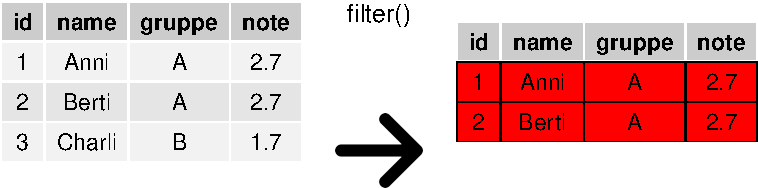
\includegraphics[width=1\linewidth,height=\textheight,keepaspectratio]{030-aufbereiten_files/figure-pdf/fig-filter-1.pdf}

}

\caption{\label{fig-filter}Sinnbild für das Filtern einer Tabelle mit
\texttt{filter}}

\end{figure}%

\begin{example}[Ob ein Foto für den Verkaufspreis nützlich
ist?]\protect\hypertarget{exm-filter}{}\label{exm-filter}

Als nächstes kommt Ihnen die Idee, mal zu schauen, ob Auktionen mit
Photo der Ware einen höheren Verkaufspreis erzielen als Auktionen ohne
Photo.

\begin{Shaded}
\begin{Highlighting}[]
\NormalTok{mariokart\_neu }\OtherTok{\textless{}{-}} \FunctionTok{filter}\NormalTok{(mariokart, stock\_photo }\SpecialCharTok{==} \StringTok{"yes"}\NormalTok{)}
\end{Highlighting}
\end{Shaded}

Sie filtern also die Tabelle so, dass \emph{nur} diese Auktionen im
Datensatz verbleiben, welche mind. ein Photo haben, mit anderen Worten,
Auktionen (Beobachtungen) bei denen gilt:
\texttt{stock\_photo\ ==\ TRUE}. \(\square\)

\end{example}

Angestachelt von Ihren Erfolgen möchten Sie jetzt komplexere Hypothesen
prüfen: Erzielen Auktionen von \emph{neuen} Spielen und zwar \emph{mit}
Photo einen höheren Preis als die übrigen Auktionen?

Anders gesagt haben Sie zwei Filterkriterien im Blick: Neuheit
\texttt{cond} und Photo \texttt{stock\_photo}. Nur diejenigen Auktionen,
die \emph{sowohl} Neuheit \emph{als auch} Photo erfüllen, möchten Sie
näher untersuchen (Filtern mit dem logischen UND):

\begin{Shaded}
\begin{Highlighting}[]
\NormalTok{mario\_filter1 }\OtherTok{\textless{}{-}} 
  \FunctionTok{filter}\NormalTok{(mariokart,  }\CommentTok{\# "\&" heißt UND:}
\NormalTok{         stock\_photo }\SpecialCharTok{==} \StringTok{"yes"} \SpecialCharTok{\&}\NormalTok{ cond }\SpecialCharTok{==} \StringTok{"new"}\NormalTok{)}
\end{Highlighting}
\end{Shaded}

Hm. Was ist mit den Auktionen, die \emph{entweder} über (mind.) ein
Photo verfügen \emph{oder auch} neu sind, oder beides (Filtern mit dem
logischen ODER)?

\begin{Shaded}
\begin{Highlighting}[]
\NormalTok{mario\_filter2 }\OtherTok{\textless{}{-}} 
  \FunctionTok{filter}\NormalTok{(mariokart,  }\CommentTok{\# "|" heißt ODER:}
\NormalTok{         stock\_photo }\SpecialCharTok{==} \StringTok{"yes"} \SpecialCharTok{|}\NormalTok{ cond }\SpecialCharTok{==} \StringTok{"new"}\NormalTok{)}
\end{Highlighting}
\end{Shaded}

Zur Erinnerung: Logische Operatoren sind in Kapitel~\ref{sec-logic}
erläutert.

\begin{exercise}[]\protect\hypertarget{exr-hyps-filter}{}\label{exr-hyps-filter}

Hier könnte man noch viele interessante Hypothesen prüfen, denken Sie
sich und tun das auch. \(\square\)

\end{exercise}

\begin{exercise}[]\protect\hypertarget{exr-filter2}{}\label{exr-filter2}

Filtern Sie die Spiele mit nur einem Lenkrad und ohne Versandkosten.
\(\square\)

\end{exercise}

\begin{exercise}[]\protect\hypertarget{exr-filter3}{}\label{exr-filter3}

Filtern Sie die Spiele mit nur einem Lenkrad, die einen
überdurchschnittlichen Verkaufspreis erzielen. Tipp: Nutzen Sie die
Funktion \texttt{describe\_distribution}, um den Mittelwert einer
Variable des Datensatzes zu erfahren (diese Funktion wohnt im R-Paket
\texttt{easystats}). \(\square\)

\end{exercise}

\subsection{\texorpdfstring{Spalten auswählen mit
\texttt{select}}{Spalten auswählen mit select}}\label{spalten-auswuxe4hlen-mit-select}

Eine Tabelle mit vielen Spalten kann schnell unübersichtlich werden. Da
lohnt es sich, eine alte goldene Regel zu beachten: Mache die Dinge so
einfach wie möglich, aber nicht einfacher. Wählen wir also \emph{nur}
die Spalten aus, die uns interessieren und entfernen wir die restlichen,
s. Abbildung~\ref{fig-select} als Beispiel.

\begin{figure}

\centering{

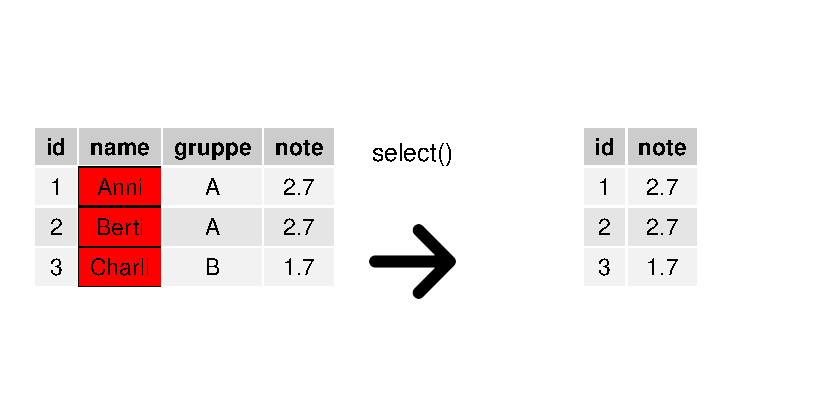
\includegraphics[width=1\linewidth,height=\textheight,keepaspectratio]{030-aufbereiten_files/figure-pdf/fig-select-1.pdf}

}

\caption{\label{fig-select}Sinnbild für das Auswählen von Spalten mit
\texttt{select}}

\end{figure}%

\begin{example}[Fokus auf nur zwei
Spalten]\protect\hypertarget{exm-select}{}\label{exm-select}

Ob wohl gebrauchte Spiele deutlich geringere Preise erzielen im
Vergleich zu neuwertigen Spielen? Sie entschließen sich, mal ein
Stündchen auf die relevanten Daten zu starren. Dafür wählen Sie mit
\texttt{select} die relevanten Spalten aus. \(\square\)

\end{example}

\begin{Shaded}
\begin{Highlighting}[]
\NormalTok{mario\_select1 }\OtherTok{\textless{}{-}} \FunctionTok{select}\NormalTok{(mariokart, cond, total\_pr)}
\end{Highlighting}
\end{Shaded}

Der Befehl \texttt{select} erwartet als Input eine Tabelle und gibt (als
Output) eine Tabelle zurück -- genau wie die meisten anderen Befehle des
Datenjudos. Auch wenn Sie nur eine Spalte auswählen, bleibt es eine
Tabelle, eben eine Tabelle mit nur einer Spalte.

\texttt{select} erlaubt Komfort; Sie können Spalten auf mehrere Arten
auswählen:

\begin{Shaded}
\begin{Highlighting}[]
\FunctionTok{select}\NormalTok{(mariokart, }\DecValTok{1}\NormalTok{, }\DecValTok{2}\NormalTok{)  }\CommentTok{\# Spalten 1 und 2}
\FunctionTok{select}\NormalTok{(mariokart, }\DecValTok{2}\SpecialCharTok{:}\DecValTok{5}\NormalTok{)  }\CommentTok{\#  Spalten 2 *bis* 5 }
\FunctionTok{select}\NormalTok{(mariokart, }\SpecialCharTok{{-}}\DecValTok{1}\NormalTok{)  }\CommentTok{\# Alle Spalte *außer* Spalte 1}
\end{Highlighting}
\end{Shaded}

\begin{exercise}[]\protect\hypertarget{exr-select}{}\label{exr-select}

Wählen Sie die Spalten \texttt{total\_pr}, \texttt{cond} sowie die
zweite Spalte der Tabelle \texttt{mariokart} aus!\footnote{\texttt{select(mariokart,\ total\_pr,\ cond,\ 2)}}
\(\square\)

\end{exercise}

Vertiefte Informationen zum Auswählen von Spalten mit \texttt{select}
finden sich
\href{https://tidyr.tidyverse.org/reference/tidyr_tidy_select.html}{hier}.\footnote{\url{https://tidyr.tidyverse.org/reference/tidyr_tidy_select.html}}

\subsection{\texorpdfstring{Spalten zu einer Zahl zusammenfassen mit
\texttt{summarise}}{Spalten zu einer Zahl zusammenfassen mit summarise}}\label{spalten-zu-einer-zahl-zusammenfassen-mit-summarise}

\begin{example}[Was ist der mittlere
Verkaufspreis?]\protect\hypertarget{exm-summarise}{}\label{exm-summarise}

Mit \texttt{summarise}, s. Listing~\ref{lst-summarise}, können wir den
mittleren Verkaufspreis der Mariokart-Spiele berechnen (50). \(\square\)

\end{example}

So eine lange Spalte mit Zahlen -- mal ehrlich: Wer blickt da schon
durch? Machen wir uns das Leben leichter, indem wir eine lange Spalte
mit Zahlen zu einer einzigen Zahl zusammenfassen. Sagen wir, drei
Studierende -- Anni, Berti, Charli -- haben eine Statistikklausur
geschrieben. Die Noten waren 2.7, 2.7 und 1.7. Damit lag der
Notenschnitt (der Mittelwert) bei 2.4; s. Abbildung~\ref{fig-summarise}.

\begin{figure}

\centering{

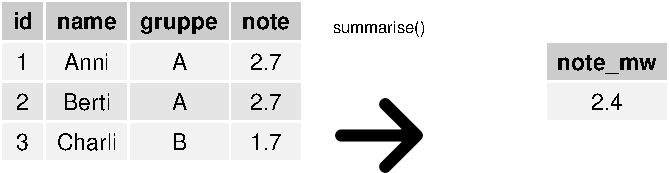
\includegraphics[width=1\linewidth,height=\textheight,keepaspectratio]{030-aufbereiten_files/figure-pdf/fig-summarise-1.pdf}

}

\caption{\label{fig-summarise}Spalten zu einer einzelnen Zahl
zusammenfassen mit \texttt{summarise}}

\end{figure}%

Fassen wir als Nächstes die Spalte \texttt{total\_pr} zu einer Zahl
zusammen, und zwar zum Mittelwert. Dann wissen wir, für welchen Preis
ein Spiel im Durchschnitt verkauft wird, s. Listing~\ref{lst-summarise}.

\begin{codelisting}

\caption{\label{lst-summarise}Die R-Funktion summarise fasst einen
Vektor z u einer Zahl zusammen}

\centering{

\begin{Shaded}
\begin{Highlighting}[]
\NormalTok{mariokart\_mittelwert }\OtherTok{\textless{}{-}} \FunctionTok{summarise}\NormalTok{(mariokart,}
                                  \AttributeTok{preis\_mw =} \FunctionTok{mean}\NormalTok{(total\_pr))}
\NormalTok{mariokart\_mittelwert}
\end{Highlighting}
\end{Shaded}

}

\end{codelisting}%

\begin{longtable}[]{@{}r@{}}
\toprule\noalign{}
preis\_mw \\
\midrule\noalign{}
\endhead
\bottomrule\noalign{}
\endlastfoot
50 \\
\end{longtable}

Aha! Etwa 50 € erzielt so eine Auktion im Schnitt.

Ein bisschen abstrakter gesprochen fasst \texttt{summarise} eine
\emph{Spalte} zu einer (einzelnen) \emph{Zahl} zusammen, s.
Abbildung~\ref{fig-desk-summ}.

\begin{figure}

\centering{

\includegraphics[width=0.25\linewidth,height=\textheight,keepaspectratio]{img/desk-stats-zsmnfassen-crop.png}

}

\caption{\label{fig-desk-summ}\texttt{summarise} fasst eine Spalte (oder
mehrere) zu einer einzelnen Zahl zusammen}

\end{figure}%

\emph{Auf welche Art} zusammengefasst werden soll, z.B. anhand des
Mittelwerts oder Maximalwerts, muss noch zusätzlich innerhalb von
\texttt{summarise} angegeben werden.

\begin{exercise}[]\protect\hypertarget{exr-summarise}{}\label{exr-summarise}

Identifizieren Sie den höchsten Kaufpreis eines
Mariokart-Spiels!\footnote{\texttt{summarise(mariokart,\ hoechster\_preis\ =\ max(total\_pr))}}
\(\square\)

\end{exercise}

\begin{exercise}[]\protect\hypertarget{exr-summarise2}{}\label{exr-summarise2}

Identifizieren Sie den Mittelwert der Versandkostenpauschale!\footnote{\texttt{summarise(mariokart,\ mw\_versand\ =\ mean(total\_pr))}}
\(\square\)

\end{exercise}

\subsection{Tabelle gruppieren}\label{tabelle-gruppieren}

Es ist ja gut und schön, zu wissen, was so ein Spiel im Schnitt kostet.
Aber viel interessanter wäre es doch, denken Sie sich, zu wissen, ob die
neuen Spiele im Schnitt mehr kosten als die alten? Ob R Ihnen so etwas
ausrechnen kann?

\begin{quote}
{\emoji{student}} Hallo R, kannst du mir die mittleren Verkaufspreise
von alten und neuen Spielen ausrechnen?
\end{quote}

\begin{quote}
{\emoji{robot}} Ich tue fast alles für dich. {\emoji{heart}}
\end{quote}

Also gut, R, dann gruppiere die Tabelle, s. Abbildung~\ref{fig-group}.

\begin{figure}

\centering{

\includegraphics[width=1\linewidth,height=\textheight,keepaspectratio]{030-aufbereiten_files/figure-pdf/fig-group-1.pdf}

}

\caption{\label{fig-group}Gruppieren von Datensätzen mit
\texttt{group\_by}}

\end{figure}%

Durch das Gruppieren wird die Tabelle in \enquote{Teiltabellen} --
entsprechend der Gruppen -- aufgeteilt. Das sieht man der R-Tabelle aber
nicht wirklich an. Aber alle nachfolgenden Berechnungen werden \emph{für
jede Teiltabelle} einzeln ausgeführt.

\begin{example}[Mittlerer Preis pro
Gruppe]\protect\hypertarget{exm-groupby}{}\label{exm-groupby}

Gruppieren alleine liefert Ihnen zwei (oder mehrere) Teiltabellen, etwa
neue Spiele (Gruppe 1, \texttt{new}) vs.~gebrauchte Spiele (Gruppe 2,
\texttt{used}). Mit anderen Worten: Wir gruppieren anhand der Variable
\texttt{cond}.

\begin{Shaded}
\begin{Highlighting}[]
\NormalTok{mariokart\_gruppiert }\OtherTok{\textless{}{-}} \FunctionTok{group\_by}\NormalTok{(mariokart, cond)}
\end{Highlighting}
\end{Shaded}

Wenn Sie die neue Tabelle betrachte, sehen Sie wenig Aufregendes, nur
einen Hinweis, dass die Tabelle gruppiert ist. Jetzt können Sie an jeder
Teiltabelle Ihre weiteren Berechnungen vornehmen, etwa die Berechnung
des mittleren Verkaufspreises.

\begin{Shaded}
\begin{Highlighting}[]
\FunctionTok{summarise}\NormalTok{(mariokart\_gruppiert, }\AttributeTok{preis\_mw =} \FunctionTok{mean}\NormalTok{(total\_pr))}
\end{Highlighting}
\end{Shaded}

\begin{longtable}[]{@{}lr@{}}
\toprule\noalign{}
cond & preis\_mw \\
\midrule\noalign{}
\endhead
\bottomrule\noalign{}
\endlastfoot
new & 54 \\
used & 47 \\
\end{longtable}

Ah, die neuen Spiele sind teuerer, wer hätt's gedacht! Langsam fühlen
Sie sich wie ein Datenchecker \ldots{} \(\square\)

\end{example}

\begin{exercise}[]\protect\hypertarget{exr-groupby}{}\label{exr-groupby}

~

\textbf{Aufgabe} Berechnen Sie den mittleren und maximalen Verkaufspreis
getrennt für Spiele mit und ohne Foto!

\textbf{Lösung}

\begin{Shaded}
\begin{Highlighting}[]
\NormalTok{mariokart\_gruppiert\_foto }\OtherTok{\textless{}{-}} \FunctionTok{group\_by}\NormalTok{(mariokart, stock\_photo)}

\NormalTok{mariokart\_verkaufspreis\_foto }\OtherTok{\textless{}{-}} 
  \FunctionTok{summarise}\NormalTok{(mariokart\_gruppiert\_foto,}
            \AttributeTok{total\_pr\_avg =} \FunctionTok{mean}\NormalTok{(total\_pr),}
            \AttributeTok{total\_pr\_max =} \FunctionTok{max}\NormalTok{(total\_pr))}

\NormalTok{mariokart\_verkaufspreis\_foto}
\end{Highlighting}
\end{Shaded}

\begin{longtable}[]{@{}lrr@{}}
\toprule\noalign{}
stock\_photo & total\_pr\_avg & total\_pr\_max \\
\midrule\noalign{}
\endhead
\bottomrule\noalign{}
\endlastfoot
no & 54 & 327 \\
yes & 48 & 75 \\
\end{longtable}

Bei Auktionen mit Foto wird im Schnitt ein höherer Preis erzielt als
ohne Foto. \(\square\)

\end{exercise}

\subsection{\texorpdfstring{Spalten verändern mit
\texttt{mutate}}{Spalten verändern mit mutate}}\label{spalten-veruxe4ndern-mit-mutate}

Immer mal wieder möchte man \emph{Spalten verändern}, bzw. deren Werte
umrechnen, s. Abbildung~\ref{fig-mutate}.

\begin{figure}

\centering{

\includegraphics[width=1\linewidth,height=\textheight,keepaspectratio]{030-aufbereiten_files/figure-pdf/fig-mutate-1.pdf}

}

\caption{\label{fig-mutate}Spalten verändern/neu berechnen mit
\texttt{mutate}}

\end{figure}%

\begin{example}[]\protect\hypertarget{exm-mutate}{}\label{exm-mutate}

Der Hersteller des Computerspiels \emph{Mariokart} kommt aus Japan;
daher erscheint es Ihnen opportun für ein anstehendes Meeting mit dem
Hersteller die Verkaufspreise von Dollar in japanische Yen umzurechnen.
Nach etwas Googeln finden Sie einen Umrechnungskurs von 1:133.

\begin{Shaded}
\begin{Highlighting}[]
\NormalTok{mariokart\_yen }\OtherTok{\textless{}{-}} 
  \FunctionTok{mutate}\NormalTok{(mariokart, }\AttributeTok{total\_pr\_yen =}\NormalTok{ total\_pr }\SpecialCharTok{*} \DecValTok{133}\NormalTok{)}
\NormalTok{mariokart\_yen }\OtherTok{\textless{}{-}} \FunctionTok{select}\NormalTok{(mariokart\_yen, total\_pr\_yen, total\_pr)}
\NormalTok{mariokart\_yen }\SpecialCharTok{|\textgreater{}} \FunctionTok{head}\NormalTok{()  }\CommentTok{\# nur die ersten paar Zeilen}
\end{Highlighting}
\end{Shaded}

\begin{longtable}[]{@{}rr@{}}
\toprule\noalign{}
total\_pr\_yen & total\_pr \\
\midrule\noalign{}
\endhead
\bottomrule\noalign{}
\endlastfoot
6856 & 52 \\
4926 & 37 \\
6052 & 46 \\
5852 & 44 \\
9443 & 71 \\
5985 & 45 \\
\end{longtable}

Sicherlich werden Sie Ihre Gesprächspartner beeindrucken. \(\square\)

\end{example}

Mit \texttt{mutate} berechnen Sie eine Spalte \texttt{x} (in einer
Tabelle) neu. Die Funktion, die Sie in \texttt{mutate} benennen wird für
jede Zeile der Spalte \texttt{x} angewendet.

\begin{example}[Beispiele für Funktionen für
\texttt{mutate}]\protect\hypertarget{exm-mutate2}{}\label{exm-mutate2}

\texttt{mutate} eignet sich, z.B. um Spalten zu addieren, zu
multiplizieren oder sonst wie zu transformieren (z.B. den Logarithmus
anwenden oder den Mittelwert der Spalte von jeder Zeile abziehen).
\(\square\)

\end{example}

\subsection{\texorpdfstring{Zeilen zählen mit
\texttt{count}}{Zeilen zählen mit count}}\label{zeilen-zuxe4hlen-mit-count}

Arbeitet man mit nominalskalierten Daten, ist (fast) alles, was man tun
kann, die entsprechenden Zeilen der Tabelle zu zählen: Man könnte z.B.
fragen, wie viele neue und wie viele alte Spiele in der Tabelle
(Dataframe) \texttt{mariokart} vorhanden sind.

\begin{example}[]\protect\hypertarget{exm-count}{}\label{exm-count}

Nach der letzten Präsentation Ihrer Analyse hat Ihre Chefin gestöhnt:
\enquote{Oh nein, alles so kompliziert. Statistik! Himmel hilf! Kann man
das nicht einfacher machen?} Anstelle von irgendwelchen komplizierten
Berechnungen (Mittelwert?) möchten Sie ihr beim nächsten Treffen nur
zeigen, wie viele Computerspiele neu und wie viele gebraucht sind (in
Ihrem Datensatz). Schlichte Häufigkeiten also. Hoffentlich ist Ihre
Chefin nicht wieder überfordert\ldots{}

\begin{Shaded}
\begin{Highlighting}[]
\NormalTok{mariocart\_counted }\OtherTok{\textless{}{-}} \FunctionTok{count}\NormalTok{(mariokart, cond)}
\NormalTok{mariocart\_counted}
\end{Highlighting}
\end{Shaded}

\begin{longtable}[]{@{}lr@{}}
\toprule\noalign{}
cond & n \\
\midrule\noalign{}
\endhead
\bottomrule\noalign{}
\endlastfoot
new & 59 \\
used & 84 \\
\end{longtable}

Aha! Es gibt mehr gebrauchte als neue Spiele. \(\square\)

\end{example}

Jetzt könnte man noch den \emph{Anteil} (engl. \emph{proportion})
ergänzen: Welcher \emph{Anteil} (der 143 Spiele in \texttt{mariokart})
ist neu, welcher gebraucht?

\begin{Shaded}
\begin{Highlighting}[]
\FunctionTok{mutate}\NormalTok{(mariocart\_counted, }\AttributeTok{Anteil =}\NormalTok{ n }\SpecialCharTok{/} \FunctionTok{sum}\NormalTok{(n))}
\end{Highlighting}
\end{Shaded}

\begin{longtable}[]{@{}lrr@{}}
\toprule\noalign{}
cond & n & Anteil \\
\midrule\noalign{}
\endhead
\bottomrule\noalign{}
\endlastfoot
new & 59 & 0.41 \\
used & 84 & 0.59 \\
\end{longtable}

\begin{exercise}[]\protect\hypertarget{exr-count}{}\label{exr-count}

Zählen Sie Sie, wie viele Auktionen ein Foto enthalten.\footnote{\texttt{count(mariokart,\ stock\_photo)}}
\(\square\)

\end{exercise}

\begin{exercise}[]\protect\hypertarget{exr-count2}{}\label{exr-count2}

Zählen Sie Sie, wie viele Auktionen ein Foto enthalten -- innerhalb der
gebrauchten Spiele und innerhalb der neuen Spiele. Anders gesagt: Teilen
Sie den Datensatz sowohl nach Zustand als auch nach Foto auf und zählen
Sie jeweils, wie viele Spiele/Auktionen in die jeweilige Gruppe
gehören.\footnote{\texttt{count(mariokart,\ stock\_photo,\ cond)}}
\(\square\)

\end{exercise}

\subsection{Fazit: Verben am
Fließband}\label{fazit-verben-am-flieuxdfband}

Die Befehle (\enquote{Verben}) des Tidyverse sind jeweils für einzelne,
typische Aufgaben des Datenaufbereitens (\enquote{Datenjudo}) zuständig.
Typischerweise erwarten diese Befehle eine Tabelle (\faIcon{table}) als
Input und liefern eine Tabelle aus Output zurück, s.
Abbildung~\ref{fig-tbl-in-out}. Die Verben des Datenjudos werden beim
\href{https://tidydatatutor.com/}{\enquote{Tidydatatutor}} anschaulich
illustriert.\footnote{\url{https://tidydatatutor.com}}

\begin{figure}

\centering{

\includegraphics[width=4in,height=0.63in]{030-aufbereiten_files/figure-latex/mermaid-figure-1.png}

}

\caption{\label{fig-tbl-in-out}Tidyverse-Befehle erwarten normalerweise
eine Tabelle (tibble) als Input und geben auch eine Tabelle zurück als
Output}

\end{figure}%

\section{Die Pfeife}\label{sec-pipe}

\href{https://en.wikipedia.org/wiki/The_Treachery_of_Images}{Das ist
keine Pfeife}, wie René Magritte 1929 in seinem
\href{https://en.wikipedia.org/wiki/File:MagrittePipe.jpg}{berühmten
Bild} schrieb, s. Abbildung~\ref{fig-pfeifen}.

\begin{figure}

\centering{

\begin{figure}[H]

\begin{minipage}{0.42\linewidth}
\pandocbounded{\includegraphics[keepaspectratio]{img/800px-Pipa_savinelli.jpg}}\end{minipage}%
%
\begin{minipage}{0.08\linewidth}

\end{minipage}%
%
\begin{minipage}{0.25\linewidth}

\%\textgreater\%

\end{minipage}%
%
\begin{minipage}{0.25\linewidth}

\textbar\textgreater{}

\end{minipage}%

\end{figure}%

}

\caption{\label{fig-pfeifen}So sieht die Pfeife in R aus (Jaja, das ist
keine Pfeife, sondern ein Symbol einer Pfeife\ldots). Links: Ein
\emph{Bild} einer Pfeife (M7, 2004). Mitte und Rechts: Die zwei
R-Symbole für eine \enquote{Pfeife} (pipe).}

\end{figure}%

\subsection{Russische Puppen}\label{russische-puppen}

Computerbefehle und im Speziellen R-Befehle kann man
\enquote{aufeinander} -- oder vielmehr: ineinander -- stapeln, so
ähnlich wie eine russische Puppe (vgl. Kapitel~\ref{sec-first-fun}).
Schauen wir uns das in einem Beispiel an. Dazu definieren wir zuerst
einen Vektor \texttt{x} aus drei Zahlen:

\begin{Shaded}
\begin{Highlighting}[]
\NormalTok{x }\OtherTok{\textless{}{-}} \FunctionTok{c}\NormalTok{(}\DecValTok{1}\NormalTok{, }\DecValTok{2}\NormalTok{, }\DecValTok{3}\NormalTok{)}
\end{Highlighting}
\end{Shaded}

Und dann kommt unser verschachtelter Befehl:

\begin{Shaded}
\begin{Highlighting}[]
\FunctionTok{sum}\NormalTok{(x }\SpecialCharTok{{-}} \FunctionTok{mean}\NormalTok{(x))}
\DocumentationTok{\#\# [1] 0}
\end{Highlighting}
\end{Shaded}

Wie schon erwähnt, arbeitet R so einen \enquote{verschachtelten} Befehl
\emph{von innen nach außen} ab:

Start: \texttt{sum(x\ -\ mean(x))}

{\(\downarrow\)}

Schritt 1: \texttt{sum(x\ -\ 2)}

{\(\downarrow\)}

Schritt 2: \texttt{sum(-1,\ 0,\ 1)}

{\(\downarrow\)}

Schritt 3: \texttt{0}. Fertig. Ganz schön kompliziert!

Soweit kann man noch einigermaßen folgen. Aber das Verschachteln kann
man noch extremer machen, dann wird's wild. Schauen Sie sich mal
folgende (Pseudo-)Syntax an:

\begin{codelisting}

\caption{\label{lst-schachtel}Eine wild verschachtelte Sequenz von
R-Befehlen}

\centering{

\begin{Shaded}
\begin{Highlighting}[]
\FunctionTok{fasse\_zusammen}\NormalTok{(}
  \FunctionTok{gruppiere}\NormalTok{(}
\NormalTok{    wähle}\FunctionTok{\_spalten}\NormalTok{(}
      \FunctionTok{filter\_zeilen}\NormalTok{(meine\_daten))))}
\end{Highlighting}
\end{Shaded}

}

\end{codelisting}%

\begin{tcolorbox}[enhanced jigsaw, leftrule=.75mm, breakable, left=2mm, colback=white, colframe=quarto-callout-caution-color-frame, opacitybacktitle=0.6, coltitle=black, colbacktitle=quarto-callout-caution-color!10!white, arc=.35mm, bottomtitle=1mm, toprule=.15mm, rightrule=.15mm, toptitle=1mm, titlerule=0mm, title=\textcolor{quarto-callout-caution-color}{\faFire}\hspace{0.5em}{Vorsicht}, bottomrule=.15mm, opacityback=0]

Ein beliebter Fehler ist es übrigens, nicht die richtige Zahl an
schließenden Klammern hinzuschreiben, z.B.
\texttt{d(c(b(a(meine\_daten))} FALSCHE ZAHL AN KLAMMERN. \(\square\)

\end{tcolorbox}

\subsection{Die Pfeife zur Rettung}\label{die-pfeife-zur-rettung}

Listing~\ref{lst-schachtel} ist schon harter Tobak, was für echte Fans.
Wäre es nicht einfacher, man könnte Listing~\ref{lst-schachtel} wie
folgt schreiben:

\begin{verbatim}
Nimm "meine_daten" *und dann*
  filter gewünschte Zeilen *und dann*
  wähle gewünschte Spalten *und dann*
  teile in Subgruppen *und dann*
  fasse sie zusammen.
\end{verbatim}

\begin{definition}[Pfeife]\protect\hypertarget{def-pipe}{}\label{def-pipe}

\enquote{Und dann} heißt auf Errisch \texttt{\%\textgreater{}\%} oder
(synonym) \texttt{\textbar{}\textgreater{}}. Man nennt diesen Befehl
\enquote{Pfeife} (engl. \emph{pipe}). \(\square\)

\end{definition}

\begin{tcolorbox}[enhanced jigsaw, leftrule=.75mm, breakable, left=2mm, colback=white, colframe=quarto-callout-note-color-frame, opacitybacktitle=0.6, coltitle=black, colbacktitle=quarto-callout-note-color!10!white, arc=.35mm, bottomtitle=1mm, toprule=.15mm, rightrule=.15mm, toptitle=1mm, titlerule=0mm, title=\textcolor{quarto-callout-note-color}{\faInfo}\hspace{0.5em}{Hinweis}, bottomrule=.15mm, opacityback=0]

Der Befehl \texttt{\%\textgreater{}\%} \emph{verknüpft} Befehle. Der
Shortcut für diesen Befehl ist Strg-Shift-M. Die Pfeife
\texttt{\%\textgreater{}\%} \enquote{wohnt} im Paket
\texttt{tidyverse}.\footnotemark{}

\end{tcolorbox}

\footnotetext{Genauer gesagt im Paket \texttt{magrittr}, welches aber
von \texttt{tidyverse} geladen wird. Also nichts, um das Sie sich
kümmern müssten.}

Mittlerweile (Seit R 4.1) ist auch im Standard-R eine Pfeife eingebaut.
Die sieht so aus: \texttt{\textbar{}\textgreater{}}. Die eingebaute
Pfeife funktioniert praktisch gleich zur anderen Pfeife
\texttt{\%\textgreater{}\%}, hat aber den Vorteil, dass Sie nicht
\texttt{tidyverse} starten müssen. Da wir \texttt{tidyverse} aber
sowieso praktisch immer starten werden, bringt es uns keinen Vorteil,
die neuere Pfeife des Standard-R \texttt{\textbar{}\textgreater{}} zu
verwenden. Aber auch keinen Nachteil. Unter \emph{Tools \textgreater{}
Global Options\ldots{}} können Sie einstellen, dass der Shortcut
Strg-Shift-M die eingebaute Pfeife verwendet.

\begin{figure}

\centering{

\includegraphics[width=4.71in,height=0.4in]{030-aufbereiten_files/figure-latex/mermaid-figure-2.png}

}

\caption{\label{fig-pfeife}Illustration für eine Pfeifensequenz, es geht
vorwärts wie am Fließband.}

\end{figure}%

\begin{codelisting}

\caption{\label{lst-pfeife}Eine Pfeifen-Befehlssequenz (Pseudo-Syntax)}

\centering{

\begin{Shaded}
\begin{Highlighting}[]
\NormalTok{meine\_daten }\SpecialCharTok{\%\textgreater{}\%}
\NormalTok{  filter\_gewünschte}\FunctionTok{\_zeilen}\NormalTok{() }\SpecialCharTok{\%\textgreater{}\%}
\NormalTok{  wähle\_gewünschte}\FunctionTok{\_spalten}\NormalTok{() }\SpecialCharTok{\%\textgreater{}\%}
  \FunctionTok{gruppiere}\NormalTok{() }\SpecialCharTok{\%\textgreater{}\%}
  \FunctionTok{fasse\_zusammen}\NormalTok{() }
\end{Highlighting}
\end{Shaded}

}

\end{codelisting}%

Und jetzt kommt's: So eine Art von Befehls-Verkettung gibt es in R.
Schauen Sie sich mal Listing~\ref{lst-pfeife} an. So eine
Pfeifen-Befehlsequenz ist ein wie ein Fließband, an dem es mehrere
Arbeitsstationen gibt, s. Abbildung~\ref{fig-pfeife}. Unser Datensatz
wird am Fließband von Station zu Station weitergereicht und an jeder
Stelle weiterverarbeitet. So könnte Ihre \enquote{Pfeifen-Sequenz} für
den Mariokart-Datensatz aussehen, s. Listing~\ref{lst-ihre-pfeife}.

\begin{codelisting}

\caption{\label{lst-ihre-pfeife}Mariokart am Fließband: Die
\enquote*{Pfeifen-Syntax}}

\centering{

\begin{Shaded}
\begin{Highlighting}[]
\CommentTok{\# Hey R, nimm die Tabelle "mariokart":}
\NormalTok{mariokart }\SpecialCharTok{\%\textgreater{}\%}  
   \CommentTok{\# filter nur die günstigen Spiele:}
  \FunctionTok{filter}\NormalTok{(total\_pr }\SpecialCharTok{\textless{}} \DecValTok{100}\NormalTok{) }\SpecialCharTok{\%\textgreater{}\%} 
  \CommentTok{\# wähle die zwei Spalten:}
  \FunctionTok{select}\NormalTok{(cond, total\_pr) }\SpecialCharTok{\%\textgreater{}\%}  
  \CommentTok{\# gruppiere die Tabelle nach Zustand des Spiels:}
  \FunctionTok{group\_by}\NormalTok{(cond) }\SpecialCharTok{\%\textgreater{}\%}  
  \CommentTok{\# fasse beide Gruppen nach dem mittleren Preis zusammen:}
  \FunctionTok{summarise}\NormalTok{(}\AttributeTok{total\_pr\_mean =} \FunctionTok{mean}\NormalTok{(total\_pr))  }
\end{Highlighting}
\end{Shaded}

}

\end{codelisting}%

\begin{longtable}[]{@{}lr@{}}
\toprule\noalign{}
cond & total\_pr\_mean \\
\midrule\noalign{}
\endhead
\bottomrule\noalign{}
\endlastfoot
new & 54 \\
used & 43 \\
\end{longtable}

Die Syntax \texttt{filter(mariokart,\ total\_pr\ \textless{}\ 100)} und
die Syntax
\texttt{mariokart\ \textbar{}\textgreater{}\ filter(total\_pr\ \textless{}\ 100)}
sind identisch. Allgemeiner: \texttt{d\ \textbar{}\textgreater{}\ f(x)}
= \texttt{f(d,\ x)}.

\section{Beispiele für
Forschungsfragen}\label{beispiele-fuxfcr-forschungsfragen}

\begin{exercise}[]\protect\hypertarget{exr-fallbsps}{}\label{exr-fallbsps}

Bevor Sie die Lösungen der folgenden Fallbeispiele lesen, versuchen Sie
die Aufgaben selbst zu lösen. Ja, ich weiß, es ist hart, nicht gleich
auf die Lösungen zu schauen! \(\square\)

\end{exercise}

Sie arbeiten als \st{Diener} strategischer Assistent der
Geschäftsführerin und sind für Faktenchecks und andere Daten-Aufgaben
zuständig. Heute sollen Sie zeigen, was Sie können (Schluck).

\begin{exercise}[Das teuerste
Spiel?]\protect\hypertarget{exr-fofrage1}{}\label{exr-fofrage1}

~

\begin{quote}
{\emoji{woman}} Ich würde von Ihnen gerne wissen, was das teuerste Spiel
ist, aber jeweils für neue und gebrauchte Spiele. Aber nur für Spiele,
die mit Foto verkauft wurden!
\end{quote}

\textbf{Lösung}

\begin{Shaded}
\begin{Highlighting}[]
\NormalTok{mariokart }\SpecialCharTok{\%\textgreater{}\%} 
  \FunctionTok{filter}\NormalTok{(stock\_photo }\SpecialCharTok{==} \StringTok{"yes"}\NormalTok{) }\SpecialCharTok{\%\textgreater{}\%} 
  \FunctionTok{group\_by}\NormalTok{(cond) }\SpecialCharTok{\%\textgreater{}\%} 
  \FunctionTok{summarise}\NormalTok{(}\AttributeTok{total\_pr\_max =} \FunctionTok{max}\NormalTok{(total\_pr))}
\end{Highlighting}
\end{Shaded}

\begin{longtable}[]{@{}lr@{}}
\toprule\noalign{}
cond & total\_pr\_max \\
\midrule\noalign{}
\endhead
\bottomrule\noalign{}
\endlastfoot
new & 75 \\
used & 62 \\
\end{longtable}

Die Funktion \texttt{max} liefert den größten Wert eines Vektors zurück:

\begin{Shaded}
\begin{Highlighting}[]
\NormalTok{x }\OtherTok{\textless{}{-}} \FunctionTok{c}\NormalTok{(}\DecValTok{1}\NormalTok{, }\DecValTok{2}\NormalTok{, }\DecValTok{10}\NormalTok{)}
\FunctionTok{max}\NormalTok{(x)}
\DocumentationTok{\#\# [1] 10}
\end{Highlighting}
\end{Shaded}

Das teuerste Spiel mit Foto kostet \texttt{75} Dollar, wenn es neu ist
und \texttt{62}, wenn es gebraucht ist. \(\square\)

\end{exercise}

\begin{exercise}[Die mittlere
Versandpauschale?]\protect\hypertarget{exr-Forschungsfrage2}{}\label{exr-Forschungsfrage2}

~

\begin{quote}
{\emoji{woman}} Ich würde gerne die mittlere Versandpauschale wissen,
aber getrennt nach Anzahl der Lenkräder, die dem Spiel beigelegt sind.
Und ich will nur Gruppen berücksichtigen, die aus mindestens 10 Spielen
bestehen!
\end{quote}

\textbf{Lösung}

Wenn wir die Anzahl der Spiele zählen in Abhängigkeit der beigelegten
Lenkräder (\texttt{wheels}), bekommen wir eine Tabelle mit zwei Spalten:
\texttt{wheels} und \texttt{n}. \texttt{n} zählt, wie viele Spiele
(Zeilen) in der jeweiligen Gruppe (\enquote{Teiltabelle}) von
\texttt{wheels} sind.

\begin{Shaded}
\begin{Highlighting}[]
\NormalTok{mariokart }\SpecialCharTok{\%\textgreater{}\%}
  \FunctionTok{count}\NormalTok{(wheels)}
\end{Highlighting}
\end{Shaded}

\begin{longtable}[]{@{}rr@{}}
\toprule\noalign{}
wheels & n \\
\midrule\noalign{}
\endhead
\bottomrule\noalign{}
\endlastfoot
0 & 37 \\
1 & 52 \\
2 & 51 \\
3 & 2 \\
4 & 1 \\
\end{longtable}

Aus dieser Tabelle sehen wir, dass 3 oder 4 Lenkräder nur selten (2 bzw.
1 Mal) beigelegt wurden und wir solche Spiele herausfiltern sollten,
bevor wir den Mittelwert der Versandkosten ausrechnen:

\begin{Shaded}
\begin{Highlighting}[]
\NormalTok{mariokart }\SpecialCharTok{\%\textgreater{}\%}
  \FunctionTok{filter}\NormalTok{(wheels }\SpecialCharTok{\textless{}} \DecValTok{3}\NormalTok{) }\SpecialCharTok{\%\textgreater{}\%} 
  \FunctionTok{group\_by}\NormalTok{(wheels) }\SpecialCharTok{\%\textgreater{}\%} 
  \FunctionTok{summarise}\NormalTok{(}\AttributeTok{mittlere\_versandkosten =} \FunctionTok{mean}\NormalTok{(ship\_pr),}
            \AttributeTok{anzahl\_spiele =} \FunctionTok{n}\NormalTok{())}
\end{Highlighting}
\end{Shaded}

\begin{longtable}[]{@{}rrr@{}}
\toprule\noalign{}
wheels & mittlere\_versandkosten & anzahl\_spiele \\
\midrule\noalign{}
\endhead
\bottomrule\noalign{}
\endlastfoot
0 & 2.7 & 37 \\
1 & 3.6 & 52 \\
2 & 2.9 & 51 \\
\end{longtable}

Die Funktion \texttt{n} gibt die Anzahl der Zeilen pro Teiltabelle
zurück.

Die mittleren Versandkosten bewegen sich also zwischen 2.7 Dollar und
3.6 Dollar, je nach Anzahl der beigelegten Lenkräder. \(\square\)

\end{exercise}

\begin{exercise}[Verkaufspreis in
Yen?]\protect\hypertarget{exr-Forschungsfrage3}{}\label{exr-Forschungsfrage3}

~

\begin{quote}
{\emoji{woman}} Ich würde gerne den Verkaufspreis in Yen wissen, nicht
in Euro. Dann rechne mal den mittleren Verkaufspreis aus und ziehe 10 \%
ab, die wir als Provision unseren Verkäufern zahlen müssen.
\end{quote}

\textbf{Lösung}

\begin{Shaded}
\begin{Highlighting}[]
\NormalTok{mariokart }\SpecialCharTok{\%\textgreater{}\%} 
  \FunctionTok{select}\NormalTok{(total\_pr) }\SpecialCharTok{\%\textgreater{}\%} 
  \FunctionTok{mutate}\NormalTok{(}\AttributeTok{total\_pr\_yen =}\NormalTok{ total\_pr }\SpecialCharTok{*} \DecValTok{133}\NormalTok{) }\SpecialCharTok{\%\textgreater{}\%} 
  \FunctionTok{summarise}\NormalTok{(}
    \AttributeTok{preis\_yen\_mw =} \FunctionTok{mean}\NormalTok{(total\_pr\_yen),}
    \AttributeTok{preis\_yen\_mw\_minus\_10proz =}\NormalTok{ preis\_yen\_mw }\SpecialCharTok{{-}} \FloatTok{0.1}\SpecialCharTok{*}\NormalTok{preis\_yen\_mw)}
\end{Highlighting}
\end{Shaded}

\begin{longtable}[]{@{}rr@{}}
\toprule\noalign{}
preis\_yen\_mw & preis\_yen\_mw\_minus\_10proz \\
\midrule\noalign{}
\endhead
\bottomrule\noalign{}
\endlastfoot
6634 & 5971 \\
\end{longtable}

Wie man sieht kann man in \texttt{summarise} auch mehr als eine
Berechnung einstellen. In diesem Fall haben wir zwei Berechnungen
angestellt: Einmal den Mittelwert und einmal den Mittelwert minus 10\%
(des Mittelwerts).

\end{exercise}

\begin{exercise}[Do It
Yourself]\protect\hypertarget{exr-diy}{}\label{exr-diy}

Denken Sie sich selber ähnliche Forschungsfragen aus. Stellen Sie diese
einer vertrauenswürdigen Kommilitonen bzw. einem vertrauenswürdigen
Kommilitonen. DIY! Schauen Sie, ob Ihre Aufgabe richtig gelöst wird.
Prüfen Sie streng\ldots{} \(\square\)

\end{exercise}

\section{Praxisbezug}\label{praxisbezug-2}

Die Covid19-Epidemie hatte weltweit massive Auswirkungen; auch
psychologischer Art wie Vereinsamung, Angst oder Depression. Mulukom et
al. (2020) berichten eine Studie, die die psychologischen Auswirkungen
untersucht; die Studie ist \href{https://osf.io/tsjnb/}{unter der
Projekt-ID \emph{tsjnb} bei der Open Science Foundation (OSF),
\textless https://osf.io/tsjnb/\textgreater, angemeldet}. Die Daten
wurden mit R ausgewertet. Beispielhaft ist unter
\url{https://osf.io/4b9p2} die R-Syntax zu sehen, die die Autoren zur
Datenaufbereitung verwendet haben. Einen guten Teil dieser Syntax kennen
Sie aus diesem Kapitel. Diese Studie ist, neben einigen vergleichbaren,
ein schönes Beispiel, wie Forschung und Praxis ineinander greifen
können: Angewandte Forschung als Beitrag zur Lösung eines akuten
Problems, der Corona-Pandemie.

\section{Wie man mit Statistik
lügt}\label{wie-man-mit-statistik-luxfcgt-1}

Ein (leider) immer mal wieder zu beobachtender \enquote{Trick}, um Daten
zu frisieren ist, nur die Daten zu berichten, die einem in den Kram
passen.

\begin{example}[]\protect\hypertarget{exm-luege-filter}{}\label{exm-luege-filter}

Eine Analystin {\emoji{woman}} möchte zeigen, dass der Verkaufspreis von
Mariokart-Spielen \enquote{viel zu niedrig} ist. Es muss ein höherer
Wert rauskommen, findet die Analystin. Der mittlere Verkaufspreis (im
Datensatz \texttt{mariokart}) liegt bei 50 Euro.

\begin{quote}
{\emoji{woman}} Kann man den Wert nicht \ldots{} \enquote{kreativ
verbessern}? Ein paar Statistik-Tricks anwenden?
\end{quote}

Um dieses Ziel zu erreichen, teilt die Analystin den Datensatz in
Gruppen nach Anzahl der dem Spiel beigelegten Lenkräder
(\texttt{wheels}). Dann wird der Mittelwert pro Gruppe berechnet.

\begin{Shaded}
\begin{Highlighting}[]
\NormalTok{mariokart\_wheels }\OtherTok{\textless{}{-}} 
\NormalTok{mariokart }\SpecialCharTok{\%\textgreater{}\%} 
  \FunctionTok{group\_by}\NormalTok{(wheels) }\SpecialCharTok{\%\textgreater{}\%} 
  \FunctionTok{summarise}\NormalTok{(}\AttributeTok{pr\_mean =} \FunctionTok{mean}\NormalTok{(total\_pr),}
            \AttributeTok{count\_n =} \FunctionTok{n}\NormalTok{())  }\CommentTok{\# \textasciigrave{}n\textasciigrave{} gibt die Anzahl der Zeilen pro Gruppe an}

\NormalTok{mariokart\_wheels}
\end{Highlighting}
\end{Shaded}

\begin{longtable}[]{@{}rrr@{}}
\toprule\noalign{}
wheels & pr\_mean & count\_n \\
\midrule\noalign{}
\endhead
\bottomrule\noalign{}
\endlastfoot
0 & 41 & 37 \\
1 & 44 & 52 \\
2 & 61 & 51 \\
3 & 70 & 2 \\
4 & 65 & 1 \\
\end{longtable}

Schließlich berechnet unsere Analystin den \emph{ungewichteten}
Mittelwert über diese 5 Gruppen:

\begin{Shaded}
\begin{Highlighting}[]
\NormalTok{mariokart\_wheels }\SpecialCharTok{\%\textgreater{}\%} 
  \FunctionTok{summarise}\NormalTok{(}\FunctionTok{mean}\NormalTok{(pr\_mean))}
\end{Highlighting}
\end{Shaded}

\begin{longtable}[]{@{}r@{}}
\toprule\noalign{}
mean(pr\_mean) \\
\midrule\noalign{}
\endhead
\bottomrule\noalign{}
\endlastfoot
56 \\
\end{longtable}

Und das Ergebnis lautet: 56 Euro! Das ist doch schon etwas
\enquote{besser} als 50 Euro.

Natürlich ist es \emph{falsch} und irreführend, hier einen ungewichteten
Mittelwert zu berechnen. Der gewichtete Mittelwert würde wiederum zum
korrekten Ergebnis, 50 Euro, führen. \(\square\)

\end{example}

\section{Fallstudien}\label{fallstudien}

\subsection{Die Pinguine}\label{die-pinguine}

\begin{figure}

\centering{

\includegraphics[width=0.5\linewidth,height=\textheight,keepaspectratio]{img/penguins.png}

}

\caption{\label{fig-penguins}Possierlich: Die Pinguine (Horst, 2024)}

\end{figure}%

\begin{exercise}[]\protect\hypertarget{exr-peng-start}{}\label{exr-peng-start}

Machen Sie sich zunächst mit dem Pinguin-Datensatz vertraut. Sie finden
den Datensatz \texttt{penguins} im R-Paket \texttt{palmerpenguins}, das
Sie auf gewohnte Art installieren können (vgl.
Kapitel~\ref{sec-install-r-pckgs}); im Internet findet man den Datensatz
auch als CSV-Datei. Fokussieren Sie Ihre Analyse auf die Zielvariable
\emph{Gewicht}. \(\square\)

\end{exercise}

Forschungsfragen:

\begin{enumerate}
\def\labelenumi{\arabic{enumi}.}
\tightlist
\item
  Was ist das mediane Gewicht von Pinguinen, gruppiert nach Spezies und
  nach Gewicht?
\item
  Wie viele Pinguine gibt es pro Spezies?
\item
  Wie viel wiegt der schwerste und der leichteste Pinguin pro Spezies?
\end{enumerate}

\subsection{Fallstudie COVIDiSTRESS}\label{fallstudie-covidistress}

\begin{figure}[H]

{\centering \includegraphics[width=0.5\linewidth,height=\textheight,keepaspectratio]{img/Covidistress1.jpg}

}

\caption{Studie COVIDiSTTRESS (Lieberoth et al., 2020)}

\end{figure}%

Lesen Sie die Beschreibung der Studie COVIDiSTRESS (Lieberoth et al.,
2022). Hier ist ein Abstract:

\begin{quote}
The COVIDiSTRESS global survey is an international collaborative
undertaking for data gathering on human experiences, behavior and
attitudes during the COVID-19 pandemic. In particular, the survey
focuses on psychological stress, compliance with behavioral guidelines
to slow the spread of Coronavirus, and trust in governmental
institutions and their preventive measures, but multiple further items
and scales are included for descriptive statistics, further analysis and
comparative mapping between participating countries. Round one data
collection was concluded May 30. 2020. To gather comparable data swiftly
from across the globe, when the Coronavirus started making a critical
impact on societies and individuals, the collaboration and survey was
constructed as an urgent collaborative process. Individual contributors
and groups in the COVIDiSTRESS network (see below) conducted
translations to each language and shared online links by their own best
means in each country.
\end{quote}

\href{https://osf.io/z39us/files/osfstorage}{Die Daten} stehen unter
\url{https://osf.io/z39us} zur freien Verfügung. Sie können diese echten
Daten eigenständig analysieren.

\section{Aufgaben}\label{aufgaben-2}

\begin{tcolorbox}[enhanced jigsaw, leftrule=.75mm, breakable, left=2mm, colback=white, colframe=quarto-callout-tip-color-frame, opacitybacktitle=0.6, coltitle=black, colbacktitle=quarto-callout-tip-color!10!white, arc=.35mm, bottomtitle=1mm, toprule=.15mm, rightrule=.15mm, toptitle=1mm, titlerule=0mm, title=\textcolor{quarto-callout-tip-color}{\faLightbulb}\hspace{0.5em}{ChatGPT}, bottomrule=.15mm, opacityback=0]

Nutzen Sie einen Chat-Bot wie ChatGPT, um sich Hilfe für die R-Syntax
geben zu lassen. \(\square\)

\end{tcolorbox}

Die Webseite \href{https://datenwerk.netlify.app}{datenwerk.netlify.app}
stellt eine Reihe von einschlägigen Übungsaufgaben bereit. Sie können
die Suchfunktion der Webseite nutzen, um die Aufgaben mit den folgenden
Namen zu suchen:

\begin{enumerate}
\def\labelenumi{\arabic{enumi}.}
\tightlist
\item
  \href{https://sebastiansauer.github.io/Datenwerk/posts/wrangle3/wrangle3.html}{wrangle3}
\item
  \href{https://sebastiansauer.github.io/Datenwerk/posts/wrangle4/wrangle4.html}{wrangle4}
\item
  \href{https://sebastiansauer.github.io/Datenwerk/posts/wrangle5/wrangle5.html}{wrangle5}
\item
  \href{https://sebastiansauer.github.io/Datenwerk/posts/wrangle7/wrangle7.html}{wrangle7}
\item
  \href{https://sebastiansauer.github.io/Datenwerk/posts/wrangle9/wrangle9.html}{wrangle9}
\item
  \href{https://sebastiansauer.github.io/Datenwerk/posts/wrangle10/wrangle10.html}{wrangle10}
\item
  \href{https://sebastiansauer.github.io/Datenwerk/posts/tidydata1/tidydata1.html}{tidydata1}
\item
  \href{https://sebastiansauer.github.io/Datenwerk/posts/affairs-dplyr/affairs-dplyr.html}{affairs-dplyr}
\item
  \href{https://sebastiansauer.github.io/Datenwerk/posts/dplyr-uebersetzen/dplyr-uebersetzen.html}{dplyr-uebersetzen}
\item
  \href{https://sebastiansauer.github.io/Datenwerk/posts/haeufigkeit01/haeufigkeit01.html}{haeufigkeit01}
\item
  \href{https://sebastiansauer.github.io/Datenwerk/posts/mariokart-mean1/mariokart-mean1.html}{mariokart-mean1}
\item
  \href{https://sebastiansauer.github.io/Datenwerk/posts/mariokart-mean2/mariokart-mean2.html}{mariokart-mean2}
\item
  \href{https://sebastiansauer.github.io/Datenwerk/posts/mariokart-mean3/mariokart-mean3.html}{mariokart-mean3}
\item
  \href{https://sebastiansauer.github.io/Datenwerk/posts/mariokart-mean4/mariokart-mean4.html}{mariokart-mean4}
\item
  \href{https://sebastiansauer.github.io/Datenwerk/posts/mariokart-max1/mariokart-max1.html}{mariokart-max1}
\item
  \href{https://sebastiansauer.github.io/Datenwerk/posts/mariokart-max2/mariokart-max2.html}{mariokart-max2}
\item
  \href{https://sebastiansauer.github.io/Datenwerk/posts/filter01/filter01.html}{filter01}
\item
  \href{https://sebastiansauer.github.io/Datenwerk/posts/affairs-dplyr/affairs-dplyr.html}{affairs-dplyr}
\item
  \href{https://sebastiansauer.github.io/Datenwerk/posts/summarise01/summarise01.html}{summarise01}
\item
  \href{https://sebastiansauer.github.io/Datenwerk/posts/summarise02/summarise02.html}{summarise02}
\item
  \href{https://sebastiansauer.github.io/Datenwerk/posts/mutate01/mutate01.html}{mutate01}
\item
  \href{https://sebastiansauer.github.io/Datenwerk/posts/wrangle3/wrangle3}{wrangle3}
\end{enumerate}

\section{Vertiefung}\label{vertiefung-3}

\subsection{Fortgeschrittenes R}\label{fortgeschrittenes-r}

\begin{tcolorbox}[enhanced jigsaw, leftrule=.75mm, breakable, left=2mm, colback=white, colframe=quarto-callout-note-color-frame, opacitybacktitle=0.6, coltitle=black, colbacktitle=quarto-callout-note-color!10!white, arc=.35mm, bottomtitle=1mm, toprule=.15mm, rightrule=.15mm, toptitle=1mm, titlerule=0mm, title=\textcolor{quarto-callout-note-color}{\faInfo}\hspace{0.5em}{Hinweis}, bottomrule=.15mm, opacityback=0]

In weiterführendem Material werden Sie immer wieder auf Inhalte treffen,
die Sie noch nicht kennen, die etwa noch nicht im Unterricht behandelt
wurden. Seien Sie unbesorgt: In der Regel können Sie diese Inhalte
einfach auslassen, ohne den Anschluss zu verlieren. Einfach ignorieren.

\end{tcolorbox}

Häufig ist es nützlich, die Werte einer Variablen umzukodieren, z.B.
\enquote{weiblich} in \enquote{w} oder in \texttt{0}. Eine gute
Möglichkeit, dies in R umzusetzen, bietet der Befehl
\texttt{case\_when}; der Befehl wohnt im Tidyverse.\footnote{\url{https://www.statology.org/dplyr-case_when/}}
Im Datenwerk finden Sie dazu Übungen, etwa
\href{https://sebastiansauer.github.io/Datenwerk/posts/mutate03/mutate03.html}{mutate03}.

\subsection{Hilfe?! Erbie!}\label{sec-erbie}

R will nicht, so wie Sie wollen? Sie haben das Gefühl, R verweigert
störrisch den Dienst, vermutlich rein aus Boshaftigkeit, rein um Sie zu
ärgern? Ausführliches Googeln und ChatGPT befragen hat keine Lösung
gebracht? Kurz, Sie brauchen die Hilfe eines kundigen Menschens?
\href{https://data-se.netlify.app/2022/01/31/erbie-einfache-reproduzierbare-beispiele-ihres-problems-mit-r-syntax/}{Sie
sollten Ihren Hilfeschrei so artikulieren}, dass er nicht nur gehört,
sondern auch verstanden wird und einen anderen Menschen veranlasst und
ermöglicht Ihnen zu helfen.

Also: Sie müssen Ihr Problem nachvollziehbar aber prägnant formulieren.
Das nennt man auch ein \emph{ERBie}, ein \emph{einfaches,
reproduzierbare Beispiel} Ihres Problems mit (R-)Syntax:

\begin{itemize}
\tightlist
\item
  \emph{einfach}: die einfachste Syntax, die Ihr Problem bzw. die
  Fehlermeldung produziert. Es bietet sich an, einen einfachen,
  allgemein bekannten Datensatz zu verwenden, etwa \texttt{mtcars}
\item
  \emph{reproduzierbar}: Code (z.B. als Textdatei oder in einem Post),
  der die Fehlermeldung entstehen lässt
\end{itemize}

\begin{example}[Beispiel für ein
Erbie]\protect\hypertarget{exm-erbie}{}\label{exm-erbie}

\emph{Problem:} Ich verstehe nicht, warum eine Fehlermeldung kommt.

\emph{Ziel:} Ich möchte die Automatikautos filtern (am = 0).

\emph{Was ich schon versucht habe:} Ich habe folgende Posts gelesen
\ldots, aber ohne Erfolg.

\emph{Erbie}:

\begin{Shaded}
\begin{Highlighting}[]
\FunctionTok{data}\NormalTok{(mtcars)}
\FunctionTok{library}\NormalTok{(dplyr)  }\CommentTok{\# nicht "tidyverse", denn "dplyr" reicht}

\NormalTok{mtcars }\SpecialCharTok{\%\textgreater{}\%} 
  \FunctionTok{filter}\NormalTok{(}\AttributeTok{am =} \DecValTok{0}\NormalTok{)  }\CommentTok{\# den kürzesten Code, der Ihren Fehler entstehen lässt!}

\FunctionTok{sessionInfo}\NormalTok{()  }\CommentTok{\# gibt Infos zur R{-}Version etc. aus}
\end{Highlighting}
\end{Shaded}

Mit dem Paket \texttt{reprex} kann man sich R-Syntax schön formuliert
ausgeben lassen. Das ist perfekt, um den Code dann in einem Forum (oder
Mail) einzustellen. Dafür müssen Sie nur den Code auswählen,
\texttt{Strg-c} drücken und dann \texttt{reprex::reprex} ausführen. Mit
\texttt{Strg-v} können Sie die schön formatierte Syntax (sowie die
Ausgabe, auch schön formatiert) dann irgendwohin pasten.

\end{example}

\begin{tcolorbox}[enhanced jigsaw, leftrule=.75mm, breakable, left=2mm, colback=white, colframe=quarto-callout-tip-color-frame, opacitybacktitle=0.6, coltitle=black, colbacktitle=quarto-callout-tip-color!10!white, arc=.35mm, bottomtitle=1mm, toprule=.15mm, rightrule=.15mm, toptitle=1mm, titlerule=0mm, title=\textcolor{quarto-callout-tip-color}{\faLightbulb}\hspace{0.5em}{Tipp}, bottomrule=.15mm, opacityback=0]

\begin{figure}[H]

\begin{minipage}{0.80\linewidth}
Posten Sie Ihr Erbie bei \url{https://gist.github.com/} als
\enquote{public gist}.
\href{https://gist.github.com/sebastiansauer/0649a0453b5cc7c6a1d16ac760667215}{Hier}
ist ein Beispiel. \(\square\)\end{minipage}%
%
\begin{minipage}{0.20\linewidth}

\begin{center}
\includegraphics[width=0.75\linewidth,height=\textheight,keepaspectratio]{030-aufbereiten_files/figure-pdf/unnamed-chunk-49-1.pdf}
\end{center}

\end{minipage}%

\end{figure}%

\end{tcolorbox}

\section{Literaturhinweise}\label{literaturhinweise-2}

Sauer (2019), Kap. 7, gibt eine Einführung in die Datenaufbereitung (mit
Hilfe von R), ähnlich zu den Inhalten dieses Kapitels. Mehr in die Tiefe
des \enquote{Datenjudo} führen ; der Autor Hadley Wickham ist in der
R-Community sehr bekannt. Er ist einer der Hauptautoren von beliebten
R-Paketen wie \texttt{dplyr} und \texttt{ggplot2}. Wickham \& Grolemund
(2018) Kap. 5 behandelt (etwas ausführlicher) die Themen dieses
Kapitels.

\part{Grundlagen des Modellieren}

\chapter{Daten verbildlichen}\label{daten-verbildlichen}

\[
\definecolor{ycol}{RGB}{230,159,0}
\definecolor{modelcol}{RGB}{86,180,233}
\definecolor{errorcol}{RGB}{0,158,115}
\definecolor{beta0col}{RGB}{213,94,0}
\definecolor{beta1col}{RGB}{0,114,178}
\definecolor{xcol}{RGB}{204,121,167}
\]

\section{Einstieg}\label{einstieg-4}

\subsection{Lernziele}\label{lernziele-4}

\begin{itemize}
\tightlist
\item
  Sie können erläutern, wann und wozu das Visualisieren statistischer
  Inhalte sinnvoll ist.
\item
  Sie kennen typische Arten von Datendiagrammen.
\item
  Sie können typische Datendiagramme mit R visualisieren.
\item
  Sie können zentrale Ergebnisse aus Datendiagrammen herauslesen.
\end{itemize}

\subsection{Benötigte R-Pakete und
Daten}\label{benuxf6tigte-r-pakete-und-daten}

Neben den üblichen Paketen \texttt{tidyverse} und \texttt{easystats}
benötigen Sie in diesem Kapitel noch \texttt{DataExplorer} und optional
\texttt{ggpubr} und \texttt{ggstatsplot}.

\begin{Shaded}
\begin{Highlighting}[]
\FunctionTok{library}\NormalTok{(tidyverse)}
\FunctionTok{library}\NormalTok{(easystats)}
\FunctionTok{library}\NormalTok{(DataExplorer)  }\CommentTok{\# nicht vergessen zu installieren}
\FunctionTok{library}\NormalTok{(ggpubr)  }\CommentTok{\# optional, Datenvisualisierung}
\FunctionTok{library}\NormalTok{(ggstatsplot)  }\CommentTok{\# optional, Datenvisualisierung}
\end{Highlighting}
\end{Shaded}

Wir arbeiten wieder mit dem Datensatz \texttt{mariokart}, s.
Kapitel~\ref{sec-import-mariokart}.

\subsection{Wozu das alles?}\label{wozu-das-alles}

\begin{quote}
{\emoji{ninja}} Wir müssen die Galaxis retten, Kermit!
\end{quote}

\begin{quote}
{\emoji{frog}} \emph{Schlock}
\end{quote}

\section{Ein Dino sagt mehr als 1000
Worte}\label{ein-dino-sagt-mehr-als-1000-worte}

Es heißt, ein Bild sage mehr als 1000 Worte. Schon richtig, aber ein
Dinosaurier sagt auch mehr als 1000 Worte, s. Abbildung~\ref{fig-dino1}.
In Abbildung~\ref{fig-dino1} sieht man verschiedene \enquote{Bilder},
also Datensätze: etwa einen Dino und einmal einen Kreis. Obwohl die
Bilder grundverschieden sind, sind die zentralen statistischen Kennwerte
(praktisch) identisch. In dieselbe Bresche schlägt \enquote{Anscombes
Quartett} (Anscombe, 1973). Es zeigt vier Datensätze, in denen die
zentralen Statistiken fast identisch sind, also Mittelwerte, Streuungen,
Korrelationen. Aber die Streudiagramme sind grundverschieden. Anscombes
Beispiel zeigt (zugespitzt): Eine Visualisierung enthüllt, was der
Statistik (als Kennzahl) verhüllt bleibt. Statistische Diagramme können
Einblicke geben, die sich nicht (leicht) in grundlegenden Statistiken
(Kennwerten) abbilden. Unter visueller Cortex ist sehr leistungsfähig.
Wir können ohne Mühe eine große Anzahl an Informationen aufnehmen und
parallel verarbeiten. Aus diesem Grund sind Datendiagramme eine
effektive und einfache Art, aus Daten Erkenntnisse zu ziehen. Nutzen Sie
Datendiagramme umfassend; sie sind einfach zu verstehen und doch sehr
mächtig.

\begin{figure}

\centering{

\includegraphics[width=1\linewidth,height=\textheight,keepaspectratio]{040-verbildlichen_files/figure-pdf/fig-dino1-1.pdf}

}

\caption{\label{fig-dino1}Alle Diagramme haben gleiche statistische
Koeffizienten, wie Mittelwert und Streuung und Korrelation, aber die
Datengrundlage sind komplett verschieden.}

\end{figure}%

\begin{definition}[Datendiagramm]\protect\hypertarget{def-datendiagramm}{}\label{def-datendiagramm}

Ein \emph{Datendiagramm} (kurz: Diagramm) ist ein Diagramm, das Daten
und Statistiken zeigt, mit dem Zweck, Erkenntnisse daraus zu ziehen.

\end{definition}

\begin{example}[Aus der Forschung: Ein aufwändiges (und ansprechendes)
Datendiagramm]\protect\hypertarget{exm-datendiagramm}{}\label{exm-datendiagramm}

~

Auf Basis des Korruptionsindex von Transparency International (2017)
erstellt Wilke (2019/2024) ein Diagramm zum Zusammenhang vom
Entwicklungsindex (Lebenserwartung, Bildung, Einkommen; vgl. Hou et al.
(2015)) und Korruption, jeweils auf Landesebene, s.
Abbildung~\ref{fig-develop-corrupt}.

Es finden sich in der Literatur (im Internet) viele weitere Beispiele
für handwerklich meisterhaft erstelle Datendiagramme, die in vielen
Fällen mit R erstellt werden (vgl. Scherer et al., 2019).

\begin{figure}

\centering{

\includegraphics[width=0.75\linewidth,height=\textheight,keepaspectratio]{img/develop-corrupt.png}

}

\caption{\label{fig-develop-corrupt}Der Zusammenhang von
Entwicklungindex und und Korruption}

\end{figure}%

\end{example}

Abbildung~\ref{fig-many-dims} zeigt ein Bild mit mehreren (5) Variablen,
die jeweils einer \enquote{Dimension} entsprechen. Wie man (nicht)
sieht, wird es langsam unübersichtlich. Offenbar kann man in einem Bild
nicht beliebig viele Variablen sinnvoll reinquetschen. Die
\enquote{Dimensionalität} eines Diagramms hat ihre Grenzen, vielleicht
bei vier bis sechs Variablen. Möchten wir den Zusammenhang von vielen
Variablen, z.B. mehr als mher, verstehen, kommen wir mit Bildern nicht
weiter. Dann brauchen wir andere Werkzeuge: Statistik, komm zu Hilfe.
Bei klaren Zusammenhängen und wenig Variablen braucht man keine
(aufwändige) Statistik. Ein Bild, also ein Datendiagramm, ist dann oft
ausreichend. Man könnte sagen, dass es Statistik nur deshalb gibt, weil
unser Auge mit mehr als ca. vier bis sechs Variablen nicht gleichzeitig
umgehen kann.

\begin{figure}

\centering{

\includegraphics[width=0.75\linewidth,height=\textheight,keepaspectratio]{040-verbildlichen_files/figure-pdf/fig-many-dims-1.pdf}

}

\caption{\label{fig-many-dims}Ein Diagramm kann nur eine begrenzte
Anzahl von Variablen zeigen. Wenn Sie dieses Bild nicht checken: Prima.
Genau das soll das Bild zeigen.}

\end{figure}%

\begin{exercise}[]\protect\hypertarget{exr-anz-dims}{}\label{exr-anz-dims}

Wie viele Variablen sind in Abbildung~\ref{fig-many-dims}
dargestellt?\footnote{5}

\end{exercise}

\section{Nomenklatur von
Datendiagrammen}\label{nomenklatur-von-datendiagrammen}

Tabelle~\ref{tbl-nom-plots} zeigt eine -- sehr kurze Nomenklatur -- von
Datendiagrammen. Weitere Nomenklaturen sind möglich, aber wir halten
hier die Sache einfach. Wer an Vertiefung interessiert ist, findet bei
data-to-vis einen Überblick über verschiedene Typen an Diagrammen, sogar
in Form einer systematischen Nomenklatur:
\url{https://www.data-to-viz.com/}.

\begin{longtable}[]{@{}
  >{\raggedright\arraybackslash}p{(\linewidth - 4\tabcolsep) * \real{0.2143}}
  >{\raggedright\arraybackslash}p{(\linewidth - 4\tabcolsep) * \real{0.3571}}
  >{\raggedright\arraybackslash}p{(\linewidth - 4\tabcolsep) * \real{0.4286}}@{}}

\caption{\label{tbl-nom-plots}Ein (sehr kurze) Nomenklatur von
Datendiagrammen}

\tabularnewline

\toprule\noalign{}
\begin{minipage}[b]{\linewidth}\raggedright
Erkenntnisziel
\end{minipage} & \begin{minipage}[b]{\linewidth}\raggedright
qualitativ
\end{minipage} & \begin{minipage}[b]{\linewidth}\raggedright
quantitativ
\end{minipage} \\
\midrule\noalign{}
\endhead
\bottomrule\noalign{}
\endlastfoot
Verteilung & Balkendiagramm & Histogramm und Dichtediagramm \\
Zusammenhang & gefülltes Balkendiagramm & Streudiagramm \\
Unterschied & gefülltes Balkendiagramm & Boxplot \\

\end{longtable}

\section{Verteilungen verbildlichen}\label{verteilungen-verbildlichen}

\subsection{Verteilung einer nominalen
Variable}\label{verteilung-einer-nominalen-variable}

\begin{definition}[Verteilung]\protect\hypertarget{def-verteilung}{}\label{def-verteilung}

Eine (Häufigkeits-)Verteilung einer Variablen \(X\) schlüsselt auf, wie
häufig jede Ausprägung von \(X\) ist. \(\square\)

\end{definition}

\begin{example}[]\protect\hypertarget{exm-verteilung1}{}\label{exm-verteilung1}

Tabelle~\ref{tbl-wheels-n} zeigt die Häufigkeitsverteilung von
\texttt{cond} (condition, also der Zustand des Artikels, neu oder
gebraucht) aus dem Datensatz \texttt{mariokart}. Die Variable hat 5
Ausprägungen; z.B. kommt die Ausprägung \texttt{new} 59 mal vor.
\(\square\)

\end{example}

\begin{longtable}[]{@{}ll@{}}

\caption{\label{tbl-wheels-n}Häufigkeitsverteilung von \texttt{cond} aus
dem Datensatz \texttt{mariokart}}

\tabularnewline

\toprule\noalign{}
cond & n \\
\midrule\noalign{}
\endhead
\bottomrule\noalign{}
\endlastfoot
new & 59 \\
used & 84 \\

\end{longtable}

Zugegeben, das Datendiagramm von \texttt{cond} ist nicht so aufregend,
s. Abbildung~\ref{fig-mario-n-plot-cond}. Wie man sieht, besteht so ein
Diagramm aus \emph{Balken}, daher heißt es \emph{Balkendiagramm}
(synonym: Säulendiagramm). Man kann so ein Diagramm um 90° drehen; keine
Ausrichtung ist grundsätzlich besser als die andere.

\begin{definition}[Balkendiagramm]\protect\hypertarget{def-balken}{}\label{def-balken}

Ein Balkendiagramm ist eine grafische Darstellung von Werten, zumeist
für die Häufigkeiten bestimmter Kategorien, also Ausprägungen nominaler
Variablen. Dabei werden rechteckige Balken verwendet, und die Länge
eines Balkens ist proportional zur dargestellten Häufigkeit. \(\square\)

\end{definition}

\begin{figure}

\begin{minipage}{0.50\linewidth}

\centering{

\includegraphics[width=0.75\linewidth,height=\textheight,keepaspectratio]{040-verbildlichen_files/figure-pdf/fig-mario-n-plot-cond-1.pdf}

}

\subcaption{\label{fig-mario-n-plot-cond-1}horizontale Balken}

\end{minipage}%
%
\begin{minipage}{0.50\linewidth}

\centering{

\includegraphics[width=0.75\linewidth,height=\textheight,keepaspectratio]{040-verbildlichen_files/figure-pdf/fig-mario-n-plot-cond-2.pdf}

}

\subcaption{\label{fig-mario-n-plot-cond-2}vertikale Balken}

\end{minipage}%

\caption{\label{fig-mario-n-plot-cond}Häufigkeitsverteilung der Variable
\texttt{cond}}

\end{figure}%

Es gibt viele Methoden, sich mit R ein Balkendiagramm ausgeben zu
lassen. Eine einfache, komfortable ist die mit dem Paket
\texttt{DataExplorer}, s. Abbildung~\ref{fig-mario-n-plot-cond}; wir
betrachten gleich die Syntax. Zuerst importieren wir die Daten, s.
Listing~\ref{lst-mariokart}. Außerdem nicht vergessen, das Paket
\texttt{DataExplorer} mit dem Befehl \texttt{library} zu starten.
(Natürlich müssen Sie das Paket einmalig installiert haben, bevor Sie es
starten können.) In diesem Paket \enquote{wohnen} die Befehle, die wir
zum Erstellen der Datendiagramme nutzen werden. Listing~\ref{lst-de1}
zeigt die Syntax, um ein Balkendiagramm zu erstellen. Auf der Hilfeseite
der Funktion finden Sie weitere Details zur Funktion.

\begin{codelisting}

\caption{\label{lst-de1}Syntax zur Erstellung eines Balkendiagramms}

\centering{

\begin{Shaded}
\begin{Highlighting}[]
\FunctionTok{library}\NormalTok{(DataExplorer)}

\NormalTok{mariokart }\SpecialCharTok{\%\textgreater{}\%} 
  \FunctionTok{select}\NormalTok{(cond) }\SpecialCharTok{\%\textgreater{}\%} 
  \FunctionTok{plot\_bar}\NormalTok{()}
\end{Highlighting}
\end{Shaded}

}

\end{codelisting}%

\begin{figure}[H]

\centering{

\includegraphics[width=0.5\linewidth,height=\textheight,keepaspectratio]{040-verbildlichen_files/figure-pdf/fig-de1-1.pdf}

}

\caption{\label{fig-de1}Ein Balkendiagramm. Unglaublich.}

\end{figure}%

Die Syntax ist in Listing~\ref{lst-de1} abgedruckt (Zur Erinnerung:
\texttt{\%\textgreater{}\%} nennt man die \enquote{Pfeife und lässt sich
als}und dann'' übersetzen, vgl. Kapitel~\ref{sec-pipe}). Übersetzen wir
die Syntax ins Deutsche:

\begin{verbatim}
Nimm den Datensatz `mariokart` *und dann*
  wähle die Spalte cond *und dann*
  zeichne ein Balkendiagramm. Fertig!
\end{verbatim}

\begin{exercise}[Spalten wählen für das
Balkendiagramm]\protect\hypertarget{exr-de1}{}\label{exr-de1}

Hätten wir andere Spalten ausgewählt, so würde das Balkendiagramm die
Verteilung jener Variablen zeigen. Ja, Sie können auch mehrere Variablen
auf einmal auswählen. Probieren Sie das doch mal aus! \(\square\)

\end{exercise}

\begin{exercise}[Visualisieren Sie die Verteilung von
\texttt{stock\_photo}!]\protect\hypertarget{exr-balken}{}\label{exr-balken}

Erstellen Sie ein geeignetes Diagramm, um die Häufigkeit jeder
Ausprägung von \texttt{stock\_photo} (Datensatz \texttt{mariokart})
darzustellen.

\textbf{Lösung}

\begin{Shaded}
\begin{Highlighting}[]
\NormalTok{mariokart }\SpecialCharTok{|\textgreater{}} 
  \FunctionTok{select}\NormalTok{(stock\_photo) }\SpecialCharTok{|\textgreater{}} 
  \FunctionTok{plot\_bar}\NormalTok{()}
\end{Highlighting}
\end{Shaded}

Mit \texttt{plot\_bar} aus \texttt{DataExplorer} kann man
Balkendiagramme darstellen. \(\square\)

\end{exercise}

\subsection{Verteilung einer quantitativen
Variable}\label{verteilung-einer-quantitativen-variable}

Bei einer quantitativen Variablen mit vielen Ausprägungen wäre ein
Balkendiagramm nicht so aussagekräftig, s.
Abbildung~\ref{fig-balken-hist} (links). Es gibt einfach zu viele
Ausprägungen.

Die Lösung: Wir reduzieren die Anzahl der Ausprägungen, in dem wir auf
ganze Dollar runden. Oder, um noch weniger Ausprägungen zu bekommen,
können wir einfach Gruppen definieren, z.B.

\begin{itemize}
\tightlist
\item
  Gruppe 1: 0-5 Dollar
\item
  Gruppe 2: 6-10 Dollar
\item
  Gruppe 3: 11-15 Dollar
\item
  \ldots{}
\end{itemize}

In Abbildung~\ref{fig-balken-hist} (rechts) sind z.B. die Ausprägungen
des Verkaufspreises (\texttt{total\_pr}) in Gruppen der Breite von 5
Dollar aufgeteilt worden. Zusätzlich sind noch die einzelnen Werte als
schwarze Punkte gezeigt.

\begin{figure}

\begin{minipage}{0.50\linewidth}

\centering{

\includegraphics[width=1\linewidth,height=\textheight,keepaspectratio]{040-verbildlichen_files/figure-pdf/fig-balken-hist-1.pdf}

}

\subcaption{\label{fig-balken-hist-1}Balkendiagramm}

\end{minipage}%
%
\begin{minipage}{0.50\linewidth}

\centering{

\includegraphics[width=1\linewidth,height=\textheight,keepaspectratio]{040-verbildlichen_files/figure-pdf/fig-balken-hist-2.pdf}

}

\subcaption{\label{fig-balken-hist-2}Histogramm}

\end{minipage}%

\caption{\label{fig-balken-hist}Balkendiagramm vs.~Histogramm für den
Gesamtpreis (\texttt{total\_pr})}

\end{figure}%

\begin{definition}[Histogramm]\protect\hypertarget{def-histogramm}{}\label{def-histogramm}

Ein Histogramm ist ein Diagramm zur Darstellung der
Häufigkeitsverteilung einer quantitativen Variablen. Die Daten werden in
Gruppen (Klassen) eingeteilt, die dann durch einen Balken (pro Klasse)
dargestellt werden. Die Höhe der Balken zeigt die Häufigkeit der Daten
in dieser Gruppe/in diesem Balken (bei konstanter Balkenbreite).

\end{definition}

Es gibt keine klare Regel, in wie viele Balken ein Histogramm gegliedert
sein sollte. Nur: Es sollten werder sehr viele noch zu wenige sein, s.
Abbildung~\ref{fig-zu-wenig-viele} (links) bzw.
Abbildung~\ref{fig-zu-wenig-viele} (rechts). Zur Erstellung eines
Histogramms können Sie die Syntax Listing~\ref{lst-de2} nutzen, vgl.
Abbildung~\ref{fig-de-hist-density}, links.

\begin{figure}

\begin{minipage}{0.50\linewidth}

\centering{

\includegraphics[width=1\linewidth,height=\textheight,keepaspectratio]{040-verbildlichen_files/figure-pdf/fig-zu-wenig-viele-1.pdf}

}

\subcaption{\label{fig-zu-wenig-viele-1}Zu viele Gruppen (Balken)}

\end{minipage}%
%
\begin{minipage}{0.50\linewidth}

\centering{

\includegraphics[width=1\linewidth,height=\textheight,keepaspectratio]{040-verbildlichen_files/figure-pdf/fig-zu-wenig-viele-2.pdf}

}

\subcaption{\label{fig-zu-wenig-viele-2}Zu wenige Gruppen (Balken)}

\end{minipage}%

\caption{\label{fig-zu-wenig-viele}Nicht zu wenig und nicht zu viele
Balken im Histogramm}

\end{figure}%

\begin{codelisting}

\caption{\label{lst-de2}Syntax zur Erstellung eines Histogramms}

\centering{

\begin{Shaded}
\begin{Highlighting}[]
\NormalTok{mariokart }\SpecialCharTok{\%\textgreater{}\%} 
  \FunctionTok{select}\NormalTok{(total\_pr) }\SpecialCharTok{\%\textgreater{}\%} 
  \FunctionTok{filter}\NormalTok{(total\_pr }\SpecialCharTok{\textless{}} \DecValTok{100}\NormalTok{) }\SpecialCharTok{\%\textgreater{}\%}  \CommentTok{\# ohne Extremwerte}
  \FunctionTok{plot\_histogram}\NormalTok{()}
\end{Highlighting}
\end{Shaded}

}

\end{codelisting}%

\begin{figure}

\begin{minipage}{0.50\linewidth}

\centering{

\includegraphics[width=1\linewidth,height=\textheight,keepaspectratio]{040-verbildlichen_files/figure-pdf/fig-de-hist-density-1.pdf}

}

\subcaption{\label{fig-de-hist-density-1}Histogramm}

\end{minipage}%
%
\begin{minipage}{0.50\linewidth}

\centering{

\includegraphics[width=1\linewidth,height=\textheight,keepaspectratio]{040-verbildlichen_files/figure-pdf/fig-de-hist-density-2.pdf}

}

\subcaption{\label{fig-de-hist-density-2}Dichtediagramm}

\end{minipage}%

\caption{\label{fig-de-hist-density}Eine stetige Verteilung
verbildlichen}

\end{figure}%

Abbildung~\ref{fig-balken-total-pr-hist-dens} fügt zum Histogramm ein
\emph{Dichtediagramm} hinzu (durchgezogene Linie). Ein Dichtediagramm
ähnelt einem \enquote{glattgeschmirgelten} Histogramm.

\begin{definition}[Dichtediagramm]\protect\hypertarget{def-dichtediagramm}{}\label{def-dichtediagramm}

Ein Dichtediagramm visualisiert die Verteilung einer stetigen Variablen.
Im Gegensatz zum Histogramm wird der Verlauf der Kurve geglättet, so
kann Rauschen (Zufallsschwankung) besser ausgeblendet werden. (Mit
\emph{Dichte} ist die relative Anzahl der Beobachtungen pro Einheit der
Variablen auf der X-Achse gemeint.)

\end{definition}

\begin{figure}

\centering{

\includegraphics[width=0.75\linewidth,height=\textheight,keepaspectratio]{040-verbildlichen_files/figure-pdf/fig-balken-total-pr-hist-dens-1.pdf}

}

\caption{\label{fig-balken-total-pr-hist-dens}Histogramm (graue Balken)
und Dichtediagramm (orange Linie) für \texttt{total\_pr}}

\end{figure}%

\begin{exercise}[]\protect\hypertarget{exr-plot-density}{}\label{exr-plot-density}

Erstellen Sie das Diagramm Abbildung~\ref{fig-de-hist-density}, rechtes
Teildiagramm!\footnote{Grob gesagt:
  \texttt{mariokart\ \%\textgreater{}\%\ plot\_density()}.}\(\square\)

\end{exercise}

Verteilungen unterscheiden sich z.B. einerseits in ihrem
\enquote{typischen} oder \enquote{mittleren} Wert (vgl.
Kapitel~\ref{sec-lage}) und anderseits in ihrer Streuung (vgl.
Kapitel~\ref{sec-streuung}). (Diagramme von) Verteilungen können
symmetrisch oder schief (nicht symmetrisch) sein, s.
Abbildung~\ref{fig-symm-schief}.

\begin{figure}

\begin{minipage}{0.50\linewidth}

\centering{

\includegraphics[width=1\linewidth,height=\textheight,keepaspectratio]{040-verbildlichen_files/figure-pdf/fig-symm-schief-1.pdf}

}

\subcaption{\label{fig-symm-schief-1}Symmetrisch (Normal)}

\end{minipage}%
%
\begin{minipage}{0.50\linewidth}

\centering{

\includegraphics[width=1\linewidth,height=\textheight,keepaspectratio]{040-verbildlichen_files/figure-pdf/fig-symm-schief-2.pdf}

}

\subcaption{\label{fig-symm-schief-2}Schief}

\end{minipage}%

\caption{\label{fig-symm-schief}Symmetrische vs.~schiefe Verteilung,
verbildlicht}

\end{figure}%

Abbildung~\ref{fig-plot-distribs} zeigt verschiedene Formen von
Verteilungen. \enquote{Bimodal} meint \enquote{zweigipflig} und
\enquote{multimodal} entsprechend \enquote{mehrgipflig}.\footnote{Quelle:
  ifes/FOM Hochschule,
  \url{https://github.com/FOM-ifes/VL-Vorlesungsfolien}}

\begin{figure}

\centering{

\includegraphics[width=1\linewidth,height=\textheight,keepaspectratio]{040-verbildlichen_files/figure-pdf/fig-plot-distribs-1.pdf}

}

\caption{\label{fig-plot-distribs}Verschiedene Verteilungsformen}

\end{figure}%

\begin{exercise}[Verteilungsform von
\texttt{total\_pr}?]\protect\hypertarget{exr-verteilungsform-total-pr}{}\label{exr-verteilungsform-total-pr}

Benennen Sie die am besten passende Verteilungsform für die Variable
\texttt{total\_pr}.

\textbf{Lösung}

Die Verteilung ist rechtsschief. \(\square\)

\end{exercise}

\subsection{Spezialfall
Normalverteilung}\label{spezialfall-normalverteilung}

Eine Normalverteilung ist eine bestimmte Art von Verteilung einer
quantitativen Variablen. Aber sie ist besonders wichtig, nd wird daher
hier besonders uhervorgehoben. Eine Normalverteilung sehen Sie in
Abbildung~\ref{fig-symm-schief}, links. Die Normalverteilung ist in der
Statistik von hoher Bedeutung, da sie sich unter (recht häufigen)
Bedingungen zwangsläufig ergeben muss. Sie hat u.a. folgende
Eigenschaften:

\begin{itemize}
\tightlist
\item
  symmetrisch
\item
  glockenförmig
\item
  stetig
\item
  eingipflig (unimodal)
\item
  Mittelwert, Median und Modus sind identisch
\end{itemize}

\begin{example}[]\protect\hypertarget{exm-norm}{}\label{exm-norm}

Beispiele für normalverteilte Variablen sind Körpergröße von Männern
oder Frauen, IQ-Werte, Prüfungsergebnisse, Messfehler, Lebensdauer von
Glühbirnen, Gewichte von Brotlaiben, Milchproduktion von Kühen,
Brustumfang schottischer Soldaten (Lyon, 2014). \(\square\)

\end{example}

\begin{definition}[Normalverteilung]\protect\hypertarget{def-norm}{}\label{def-norm}

Eine Normalverteilung ist eine spezielle Art von Verteilung einer
quantitativen Variablen. Sie ist symmetrisch, glockenförmig, stetig,
unimodal und hat Mittelwert, Median und Modus identisch. Sie lässt sich
durch zwei Parameter vollständig beschreiben: Mittelwert (\(\mu\)) und
Streuung (\(\sigma\)). \(\square\)

\end{definition}

\begin{definition}[Entstehung einer
Normalverteilung]\protect\hypertarget{def-normal-galton}{}\label{def-normal-galton}

Wenn sich eine Variable \(X\) als Summe mehrerer, unabhängiger, etwa
gleich starker Summanden, dann kann man erwarten, dass sich diese
Variable \(X\) tendenziell normalverteilt. \(\square\)

\end{definition}

\begin{figure}

\begin{minipage}{0.80\linewidth}
Dieses Phänomen kann man gut anhand des
\href{https://www.youtube.com/watch?v=3m4bxse2JEQ}{Galton-Bretts}
veranschaulichen.\end{minipage}%
%
\begin{minipage}{0.20\linewidth}

\begin{center}
\includegraphics[width=0.75\linewidth,height=\textheight,keepaspectratio]{040-verbildlichen_files/figure-pdf/unnamed-chunk-17-1.pdf}
\end{center}

\end{minipage}%

\end{figure}%

Eine Normalverteilung lässt sich exakt beschreiben anhand zweier
Parameter: ihres zentralen Werts (Mittelwerts), \(\mu\), und ihrer
Streuung (Standardabweichung), \(\sigma\).

Kennt man diese beiden Parameter, so kann man einfach angeben, welcher
Anteil der Fläche sich in einem bestimmten Bereich befindet, s.
Abbildung~\ref{fig-norm-perc}.

Davon leitet sich die \enquote{68-95-99.7-Prozentregel} ab:

\begin{itemize}
\tightlist
\item
  \(68\,\%\) der Werte im Bereich \(\mu\pm 1 \cdot \sigma\)
\item
  \(95\,\%\) der Werte im Bereich \(\mu\pm 2 \cdot \sigma\)
\item
  \(99{,}7\,\%\) der Werte im Bereich \(\mu\pm 3 \cdot \sigma\)
\end{itemize}

\begin{figure}

\centering{

\includegraphics[width=0.75\linewidth,height=\textheight,keepaspectratio]{img/Standard_deviation_diagram_micro.svg.png}

}

\caption{\label{fig-norm-perc}Die Flächeninhalte
(Wahrscheinlichkeitsmasse) einer Normalverteilung in Abhängigkeit der
SD-Einheiten (Ainali, 2007)}

\end{figure}%

\section{Zusammenhänge
verbildlichen}\label{zusammenhuxe4nge-verbildlichen}

\subsection{Zusammenhang nominaler
Variablen}\label{zusammenhang-nominaler-variablen}

\begin{example}[Beispiele für Zusammenhänge bei nominalen
Variablen]\protect\hypertarget{exm-nom-zshg}{}\label{exm-nom-zshg}

~

\begin{itemize}
\tightlist
\item
  Hängt Berufserfolg (Führungskraft ja/nein) mit dem Geschlecht
  zusammen?
\item
  Hängt der Beruf des Vaters mit dem Schulabschluss des Kindes (Abitur,
  Realschule, Mittelschule) zusammen?
\item
  Gibt es einen Zusammenhang zwischen Automarke und politische Präferenz
  einer Partei? \(\square\)
\end{itemize}

\end{example}

Sagen wir, Sie arbeiten immer noch beim Online-Auktionshaus und Sie
fragen sich, ob ein Produktfoto wohl primär bei neuwertigen Produkten
beiliegt, aber nicht bei gebrauchten? Dazu betrachten Sie wieder die
\texttt{mariokart}-Daten, s. Abbildung~\ref{fig-zshg-nom1}.

\begin{figure}

\begin{minipage}{0.45\linewidth}

\centering{

\includegraphics[width=1\linewidth,height=\textheight,keepaspectratio]{040-verbildlichen_files/figure-pdf/fig-zshg-nom1-1.pdf}

}

\subcaption{\label{fig-zshg-nom1-1}starker Zusammenhang}

\end{minipage}%
%
\begin{minipage}{0.10\linewidth}
~\end{minipage}%
%
\begin{minipage}{0.45\linewidth}

\centering{

\includegraphics[width=1\linewidth,height=\textheight,keepaspectratio]{040-verbildlichen_files/figure-pdf/fig-zshg-nom1-2.pdf}

}

\subcaption{\label{fig-zshg-nom1-2}schwacher Zusammenhang}

\end{minipage}%

\caption{\label{fig-zshg-nom1}Zusammenhang zwischen nominalskalierten
Variablen verbildlichen. (a) Es findet sich ein Zusammenhang von Foto
und Zustand in den Daten. (b) Es findet sich (fast) kein Zusammenhang
von \texttt{wheel} und Foto in den Daten}

\end{figure}%

Tatsächlich: Es findet sich ein Zusammenhang zwischen der Tatsache, ob
dem versteigerten Produkt ein Foto bei lag und ob es neuwertig oder
gebraucht war (Abbildung~\ref{fig-zshg-nom1}, links). Bei neuen Spielen
war fast immer (ca. 90\%) ein Foto dabei; bei gebrauchten Spielen
immerhin bei gut der Hälfte der Fälle.

Anders sieht es aus für die Frage, ob ein (oder mehrere) Lenkräder dem
Spiel beilagen (oder nicht) in Zusammenhang mit der Fotofrage Hier gab
es fast keinen Unterschied zwischen neuen und alten Spielen, was die
Frage nach \enquote{Foto des Produkts dabei} betraf
(Abbildung~\ref{fig-zshg-nom1}, rechts), der Anteil betrug jeweils ca.
70\%. Das zeigt, dass es keinen Zusammenhang zwischen Foto und
Neuwertigkeit des Spiels gibt (laut unseren Daten).

Bildlich gesprochen: Unterscheiden sich die \enquote{Füllhöhe} in den
Diagrammen, so gibt es einen Unterschied hinsichtlich \enquote{Foto ist
dabei} zwischen den beiden Gruppen (linker vs.~rechter Balken).
Unterscheiden sich die Anteile in den Gruppen (neuwertige vs.~gebrauchte
Spiele), so spielt z.B. die Variable \enquote{Foto dabei} offenbar eine
Rolle. Dann hängen Neuwertigkeit und \enquote{Foto dabei} also zusammen!

So können Sie sich in R ein gefülltes Balkendiagramm ausgeben lassen,
z.B. mit \texttt{plot\_bar(mariokart,\ by\ =\ "cond")} (Paket
\texttt{DataExplorer}). Diese Darstellung eignet sich, um Zusammenhänge
zwischen zwei zweistufigen nominalskalierten Variablen zu verbildlichen.
Die verschiedenen Werte der Füllfarbe werden den Stufen der Variablen
\texttt{cond} zugewiesen, s. Listing~\ref{lst-plot-bar}.

\begin{codelisting}

\caption{\label{lst-plot-bar}R-Syntax für ein gefülltes Balkendiagramm}

\centering{

\begin{Shaded}
\begin{Highlighting}[]
\NormalTok{mariokart }\SpecialCharTok{\%\textgreater{}\%} 
  \FunctionTok{select}\NormalTok{(cond, stock\_photo) }\SpecialCharTok{\%\textgreater{}\%} 
  \FunctionTok{plot\_bar}\NormalTok{(}\AttributeTok{by =} \StringTok{"cond"}\NormalTok{)  }\CommentTok{\# aus dem Paket DataExplorer}
\end{Highlighting}
\end{Shaded}

}

\end{codelisting}%

\emph{Gefüllte Balkendiagramme} eignen sich zur Analyse eines
Zusammenhangs zwischen nominalskalierten Variablen. Allerdings sollte
eine der beiden Variablen nur zwei Ausprägungen aufweisen, sonst sind
die Zusammenhänge nicht mehr so gut zu erkennen. Außerdem sollten die
Balken auf gleiche Länge (100\%) ausgerichtet sein.

\begin{exercise}[Zusammenhang
visualisieren]\protect\hypertarget{exr-zsmnhang-cond-wheels}{}\label{exr-zsmnhang-cond-wheels}

Visualisieren Sie den Zusammenhang der beiden nominalen Variablen
\texttt{cond} und \texttt{wheels}!

\begin{Shaded}
\begin{Highlighting}[]
\NormalTok{mariokart }\SpecialCharTok{|\textgreater{}} 
  \CommentTok{\# Mache aus einer metrischen eine nominale Variable: }
  \FunctionTok{mutate}\NormalTok{(}\AttributeTok{wheels =} \FunctionTok{factor}\NormalTok{(wheels)) }\SpecialCharTok{|\textgreater{}} 
  \FunctionTok{select}\NormalTok{(cond, wheels) }\SpecialCharTok{|\textgreater{}} 
  \FunctionTok{plot\_bar}\NormalTok{(}\AttributeTok{by =} \StringTok{"cond"}\NormalTok{)}
\end{Highlighting}
\end{Shaded}

\textbf{Lösung}

\texttt{wheels} ist als metrische Variable (\texttt{int}: Integer, d.h.
Ganzzahl) formatiert im Datensatz \texttt{mariokart}. Wir müssen Sie
zunächst als Faktorvariable umformatieren, damit R sie als nominal
skalierte Variable erkennt. \(\square\)

\end{exercise}

\subsection{Zusammenhang bei metrischen Variablen}\label{sec-zshg-metr}

Den (etwaigen) Zusammenhang zweier metrischer Variablen kann man mit
einem \emph{Streudiagramm} visualisieren (engl. scatterplot).
Abbildung~\ref{fig-streu1} links untersucht den Zusammenhang des
Einstiegpreises (X-Achse) und Abschlusspreises (Y-Achse) von Geboten bei
Versteigerungen des Computerspiels Mariokart. In dem Diagramm ist eine
\enquote{Trendgerade} (Regressionsgerade), um die Art des Zusammenhangs
besser zu verdeutlichen. Die Trendgerade steigt an (von links nach
recht). Daraus kann man schließen: Es handelt sich um einen
\emph{gleichsinnigen} (positiven) Zusammenhang: Je höher der Startpreis,
desto \emph{höher} der Abschlusspreis, zumindest tendenziell. Diese
Gerade verläuft \enquote{mittig} in den Daten (wir definieren das später
genauer). Diese Trendgerade gibt Aufschluss über \enquote{typische}
Werte: Welcher Y-Wert ist \enquote{typisch} für einen bestimmten X-Wert?
Abbildung~\ref{fig-streu1} rechts untersucht den Zusammenhang zwischen
Anzahl der Gebote (X-Achse) und Abschlusspreises (Y-Achse). Es handelt
sich um einen negativen Zusammenhang: Je mehr Gebote, desto
\emph{geringer} der Abschlusspreis. Das erkennt man an der sinkenden
Trendgeraden. Die Ellipse zeigt an, wie eng die Daten um die Trendgerade
streuen. Daraus kann man ableiten, wie stark der Absolutwert des
Zusammenhangs ist, vgl. Abbildung~\ref{fig-cors}.

\begin{figure}

\begin{minipage}{0.50\linewidth}

\centering{

\includegraphics[width=1\linewidth,height=\textheight,keepaspectratio]{040-verbildlichen_files/figure-pdf/fig-streu1-1.pdf}

}

\subcaption{\label{fig-streu1-1}positiver, mittelstarker Zusammenhang}

\end{minipage}%
%
\begin{minipage}{0.50\linewidth}

\centering{

\includegraphics[width=1\linewidth,height=\textheight,keepaspectratio]{040-verbildlichen_files/figure-pdf/fig-streu1-2.pdf}

}

\subcaption{\label{fig-streu1-2}negativer, schwacher Zusammenhang}

\end{minipage}%

\caption{\label{fig-streu1}Streudiagramm zur Darstellung eines
Zusammenhangs zweier metrischer Variablen}

\end{figure}%

\begin{definition}[Linearer
Zusammenhang]\protect\hypertarget{def-lin-zshg}{}\label{def-lin-zshg}

Lässt sich die Beziehung zwischen zwei Variablen mit einer Geraden
visualisieren, so spricht man von einem linearen Zusammenhang. Ändert
man eine der beiden Variablen um einen bestimmten Wert (z.B. 1), so
ändert sich die andere um einen proportionalen Wert (z.B. 0.5).
\(\square\)

\end{definition}

Natürlich könnte man auch nicht-lineare Zusammenhänge untersuchen, aber
der Einfachheit halber konzentrieren wir uns hier auf lineare; Beispiele
für nicht-lineare Zusammenhänge sind in Abbildung~\ref{fig-nonlinear} zu
sehen.

\begin{figure}

\centering{

\includegraphics[width=1\linewidth,height=\textheight,keepaspectratio]{040-verbildlichen_files/figure-pdf/fig-nonlinear-1.pdf}

}

\caption{\label{fig-nonlinear}Beispiele nichtlinearer Zusammenhänge}

\end{figure}%

\begin{definition}[Richtung und Stärke eines
Zusammenhang]\protect\hypertarget{def-zshg}{}\label{def-zshg}

\emph{Gleichsinnige} (positive) Zusammenhänge erkennt man an
\emph{aufsteigenden} Trendgeraden \(\nearrow\); \emph{gegensinnige}
(negative) Zusammenhänge an \emph{absteigenden} Trendgeraden
\(\searrow\). \(\square\)

\end{definition}

Starke Zusammenhänge erkennt man an schmalen Ellipsen
(\enquote{Baguette} ); schwache Zusammenhänge an breiten Ellipsen
(\enquote{Torte} ). Abbildung~\ref{fig-cors} bietet einen Überblick über
verschiedene Beispiele von Richtung und Stärke von
Zusammenhängen.\footnote{Quelle: Aufbauend auf FOM/ifes, Autor: Norman
  Markgraf} In Abbildung~\ref{fig-cors} ist für jedes Teildiagramm eine
Zahl angegeben: der \emph{Korrelationskoeffizient}. Diese Statistik
quantifiziert Richtung und Stärke des Zusammenhangs (mehr dazu in Kap.
Kapitel~\ref{sec-zusammenhaenge}). Ein positives Vorzeichen steht für
einen positiven Zusammenhang, ein negatives Vorzeichen für einen
negativen Zusammenhang. Der (Absolut-)Wert gibt die Stärke des linearen
Zusammenhangs an (Cohen, 1992):

\begin{itemize}
\tightlist
\item
  ±0: Kein Zusammenhang
\item
  ±0.1: schwacher Zusammenhang
\item
  ±0.3: mittlerer Zusammenhang
\item
  ±0.5: starker Zusammenhang
\item
  ±1: perfekter Zusammenhang
\end{itemize}

\begin{figure}

\centering{

\includegraphics[width=0.5\linewidth,height=\textheight,keepaspectratio]{040-verbildlichen_files/figure-pdf/fig-cors-1.pdf}

}

\caption{\label{fig-cors}Lineare Zusammenhänge verschiedener Stärke und
Richtung}

\end{figure}%

Abbildung~\ref{fig-cors2} hat die gleiche Aussage wie
Abbildung~\ref{fig-cors}, ist aber plakativer, indem \emph{Stärke}
(schwach, stark) und \emph{Richtung} (positiv, negativ)
gegenübergestellt sind.

\begin{figure}

\centering{

\includegraphics[width=0.75\linewidth,height=\textheight,keepaspectratio]{040-verbildlichen_files/figure-pdf/fig-cors2-1.pdf}

}

\caption{\label{fig-cors2}Überblick über starke vs.~schwache bzw.
positive vs.~negative Zusammenhänge}

\end{figure}%

Man sieht in Abbildung~\ref{fig-cors} und Abbildung~\ref{fig-cors2},
dass ein \emph{negativer} Korrelationskoeffizient mit einer
\emph{absinkenden} Trendgerade (synonym: Regressionsgerade; blaue Linie)
einhergeht. Umgekehrt geht ein \emph{positiver} Trend mit einer
\emph{ansteigenden} Trendgerade einher. Zweitens erkennt man, dass
\emph{starke} Zusammenhänge mit einer \emph{schmalen} Ellipse
einhergehen und \emph{schwache} Zusammenhänge mit einer \emph{breiten}
Ellipse einhergehen.

\begin{example}[]\protect\hypertarget{exm-scatter}{}\label{exm-scatter}

Sie arbeiten nach wie vor bei einem Online-Auktionshaus, und manchmal
gehört Datenanalyse zu Ihren Aufgaben. Daher interessiert Sie, ob welche
Variablen mit dem Abschlusspreis (\texttt{total\_pr}) im Datensatz
\texttt{mariokart} zusammenhängen. Sie verbildlichen die Daten mit R,
und zwar nutzen Sie das Paket \texttt{DataExplorer}. Außerdem müssen wir
noch die Daten importieren, falls noch nicht getan, s.
Listing~\ref{lst-mariokart}.

So, jetzt kann die eigentliche Arbeit losgehen. Da Sie sich nur auf
metrische Variablen konzentrieren wollen, wählen Sie (mit
\texttt{select}) nur diese Variablen aus. Dann weisen Sie R an, einen
Scatterplot zu malen (\texttt{plot\_scatterplot}) und zwar jeweils den
Zusammenhang einer der gewählten Variablen mit dem Abschlusspreis
(\texttt{total\_pr}), da das die Variable ist, die Sie primär
interessiert. Das Ergebnis sieht man in \textbf{?@fig-mario-scatter}.
\(\square\)

\end{example}

\begin{Shaded}
\begin{Highlighting}[]
\NormalTok{mariokart }\SpecialCharTok{\%\textgreater{}\%} 
  \FunctionTok{select}\NormalTok{(duration, n\_bids, start\_pr,}
\NormalTok{         total\_pr, wheels) }\SpecialCharTok{\%\textgreater{}\%} 
  \FunctionTok{plot\_scatterplot}\NormalTok{(}\AttributeTok{by =} \StringTok{"total\_pr"}\NormalTok{, }\AttributeTok{nrow =} \DecValTok{1}\NormalTok{)}
\end{Highlighting}
\end{Shaded}

\begin{figure}[H]

\centering{

\includegraphics[width=0.5\linewidth,height=\textheight,keepaspectratio]{040-verbildlichen_files/figure-pdf/fig-mario-scatter-1.pdf}

}

\caption{\label{fig-mario-scatter-1}Der Zusammenhang metrischer
Variablen mit Abschlusspreis}

\end{figure}%

\begin{figure}[H]

\centering{

\includegraphics[width=0.5\linewidth,height=\textheight,keepaspectratio]{040-verbildlichen_files/figure-pdf/fig-mario-scatter-2.pdf}

}

\caption{\label{fig-mario-scatter-2}Der Zusammenhang metrischer
Variablen mit Abschlusspreis}

\end{figure}%

Aha\ldots{} Was sagt uns das Bild? Hm. Es scheint einige Extremwerte zu
geben, die dafür sorgen, dass der Rest der Daten recht
zusammengequetscht auf dem Bild erscheint. Vielleicht sollten Sie solche
Extremwerte lieber entfernen? Sie entscheiden sich, nur Verkäufe mit
einem Abschlusspreis von weniger als 100 Dollar anzuschauen
(\texttt{total\_pr\ \textless{}\ 100}), s. Listing~\ref{lst-no-extreme}.

\begin{codelisting}

\caption{\label{lst-no-extreme}Mariokart ohne Extremwerte}

\centering{

\begin{Shaded}
\begin{Highlighting}[]
\NormalTok{mariokart\_no\_extreme }\OtherTok{\textless{}{-}}
\NormalTok{  mariokart }\SpecialCharTok{\%\textgreater{}\%} 
  \FunctionTok{filter}\NormalTok{(total\_pr }\SpecialCharTok{\textless{}} \DecValTok{100}\NormalTok{)}
\end{Highlighting}
\end{Shaded}

}

\end{codelisting}%

Ohne Extremwerte schält sich ein deutlicheres Bild hervor: Startpreis
(\texttt{start\_pr}) und Anzahl der Räder (\texttt{wheels}) scheinen am
stärksten mit dem Abschlusspreis zusammenzuhängen. Das Argument
\texttt{by\ =\ "total\_pr"} bei \texttt{plot\_scatterplot} weist R an,
als Y-Variable stets \texttt{total\_pr} zu verwenden. Alle übrigen
Variablen kommen jeweils einmal als X-Variable vor. \(\square\)

\begin{exercise}[Zuammenhang
visualisieren]\protect\hypertarget{exr-zsmnhang-metrisch}{}\label{exr-zsmnhang-metrisch}

Visualisieren Sie den Zusammenhang der beiden metrischen Variablen
\texttt{start\_pr} und \texttt{total\_pr}. Verwenden Sie den Datensatz
ohne Extremwerte wie oben definiert.

\textbf{Lösung}

\begin{Shaded}
\begin{Highlighting}[]
\NormalTok{mariokart\_no\_extreme }\SpecialCharTok{|\textgreater{}} 
  \FunctionTok{select}\NormalTok{(start\_pr, total\_pr) }\SpecialCharTok{|\textgreater{}} 
  \FunctionTok{plot\_scatterplot}\NormalTok{(}\AttributeTok{by =} \StringTok{"total\_pr"}\NormalTok{)}
\end{Highlighting}
\end{Shaded}

Zuerst wählt man die Spalten (mit \texttt{select}), die man
visualisieren möchte, dann ruft man die Funktion
\texttt{plot\_scatterplot} auf. \(\square\)

\end{exercise}

\section{Unterschiede verbildlichen}\label{unterschiede-verbildlichen}

\subsection{Unterschiede bei nominalen
Variablen}\label{unterschiede-bei-nominalen-variablen}

Gute Nachrichten: Für nominale Variablen bieten sich Balkendiagramme
sowohl zur Darstellung von Zusammenhängen als auch von Unterschieden an.
Genau genommen zeigt ja Abbildung~\ref{fig-zshg-nom1} (links) den
\emph{Unterschied} zwischen neuen und gebrauchten Spielen hinsichtlich
der Frage, ob Fotos beiliegen. Und wie man in
Abbildung~\ref{fig-zshg-nom1} sieht, ist der Anteil der Spiele mit Foto
bei den neuen Spielen höher als bei gebrauchten Spielen.

\subsection{Unterschiede bei quantitativen
Variablen}\label{unterschiede-bei-quantitativen-variablen}

Eine typische Analysefrage ist, ob sich zwei Gruppen hinsichtlich einer
metrischen Zielvariablen deutlich unterscheiden. Genauer gesagt
untersucht man z.B. oft, ob sich die Mittelwerte der beiden Gruppen
zwischen der Zielvariablen deutlich unterscheiden. Das hört sich
abstrakt an? Am besten wir schauen uns einige Beispiele an, s.
Abbildung~\ref{fig-compare-groups1}.

\begin{figure}

\begin{minipage}{0.50\linewidth}

\centering{

\includegraphics[width=1\linewidth,height=\textheight,keepaspectratio]{040-verbildlichen_files/figure-pdf/fig-compare-groups1-1.pdf}

}

\subcaption{\label{fig-compare-groups1-1}Histogramm pro Gruppe}

\end{minipage}%
%
\begin{minipage}{0.50\linewidth}

\centering{

\includegraphics[width=1\linewidth,height=\textheight,keepaspectratio]{040-verbildlichen_files/figure-pdf/fig-compare-groups1-2.pdf}

}

\subcaption{\label{fig-compare-groups1-2}Boxplot pro Gruppe}

\end{minipage}%

\caption{\label{fig-compare-groups1}Unterschiede zwischen zwei Gruppen:
Metrische Y-Variable, nominale X-Variable}

\end{figure}%

Das linke Teildiagramm von Abbildung~\ref{fig-compare-groups1} zeigt das
Histogramm von \texttt{total\_pr}, getrennt für neue und gebrauchte
Spiele, vgl. Abbildung~\ref{fig-de-hist-density}. Das rechte
Teildiagramm zeigt die gleichen Verteilungen, aber mit einer
vereinfachten, groberen Darstellungsform, den \emph{Boxplot}.\footnote{Übrigens:
  Freunde lassen Freunde nicht Balkendiagramme verwenden, um Mittelwerte
  darzustellen:
  \url{https://github.com/cxli233/FriendsDontLetFriends\#1-friends-dont-let-friends-make-bar-plots-for-means-separation}.}
Was ein \enquote{deutlicher} (substanzieller, bedeutsamer, relevanter
oder signifikanter) Zusammenhang ist, ist keine statistische, sondern
inhaltliche Frage, die man mit Sachverstand zum Forschungsgegenstand
beantworten muss.

\begin{definition}[Boxplot]\protect\hypertarget{def-boxplot}{}\label{def-boxplot}

Der Boxplot ist eine Vereinfachung bzw. eine Zusammenfassung eines
Histograms. Damit stellt der Boxplot auch eine Verteilung (einer
metrischen Variablen) dar. \(\square\)

\end{definition}

In Abbildung~\ref{fig-hist-to-box} sieht man die \enquote{Übersetzung}
von Histogramm (oben) zu einem Boxplot (unten). Ob der Boxplot
horizontal oder vertikal steht, ist Ihrem Geschmack überlassen.

\begin{figure}

\centering{

\includegraphics[width=1\linewidth,height=\textheight,keepaspectratio]{040-verbildlichen_files/figure-pdf/fig-hist-to-box-1.pdf}

}

\caption{\label{fig-hist-to-box}Übersetzung eines Histogramms zu einem
Boxplot}

\end{figure}%

Schauen wir uns die \enquote{Anatomie} des Boxplots näher an:

\begin{enumerate}
\def\labelenumi{\arabic{enumi}.}
\tightlist
\item
  Der \emph{dicke Strich} in der Box zeigt den Median der Verteilung,
  vgl. Kapitel~\ref{sec-median}.
\item
  Die \emph{Enden der Box} zeigen das 1. Quartil (41) bzw. das 3.
  Quartil (54). Damit zeigt die Breite der Box die Streuung der
  Verteilung an, genauer gesagt die Streuung der inneren 50\% der
  Beobachtungen. Je breiter die Box, desto größer die Streuung. Die
  Breite der Box nennt man auch den \emph{Interquartilsabstand} (IQR).
\item
  Die \enquote{\emph{Antennen}} des Boxplots zeigen die Streuung in den
  kleinsten 25\% der Werte (linke Antenne) bzw. die Streuung der größten
  25\% der Werte (rechte Antennen). Je länger die Antenne, desto größer
  die Streuung.
\item
  Falls es aber \emph{Extremwerte} gibt, so sollten die lieber einzeln,
  separat, außerhalb der Antennen gezeigt werden. Daher ist die
  Antennenlänge auf die 1,5-fache Länge der Box beschränkt. Werte die
  außerhalb dieses Bereichs liegen (also mehr als das 1,5-fache der
  Boxlänge von Q3 entfernt sind) werden mittels eines Punktes
  dargestellt.
\item
  Liegt der Median-Strich in der Mitte der Box, so ist die Verteilung
  \emph{symmetrisch} (bezogen auf die inneren 50\% der Werte), liegt der
  Median-Strich nicht in der Mitte der Box, so ist die Verteilung nicht
  symmetrisch (d.h. sie ist \emph{schief}). Gleiches gilt für die
  Antennenlängen: Sind die Antennen gleich lang, so ist der äußere Teil
  der Verteilung symmetrisch, andernfalls schief.
\end{enumerate}

\begin{example}[]\protect\hypertarget{exm-Boxplots}{}\label{exm-Boxplots}

In einer vorherigen Analyse haben Sie den Zusammenhang von
Abschlusspreis und der Anzahl der Lenkräder untersucht. Jetzt möchten
Sie eine sehr ähnliche Fragestellung betrachten: Wie
\emph{unterscheiden} sich die Verkaufspreise je nach Anzahl der
beigelegten Lenkräder? Flink erstellen Sie dazu folgendes Diagramm,
Abbildung~\ref{fig-box-wheels1}, links. Es zeigt die Verteilung des
Abschlusspreises, aufgebrochen nach Anzahl Lenkräder
(\texttt{by\ =\ "wheels"}). \(\square\)

\end{example}

Aber ganz glücklich sind Sie mit dem Diagramm nicht: R hat die Variable
\texttt{wheels} komisch aufgeteilt. Es wäre eigentlich ganz einfach,
wenn R die Gruppen \texttt{0}, \texttt{1}, \texttt{2}, \texttt{3} und
\texttt{4} aufteilen würde. Aber schaut man sich die Y-Achse (im linken
Teildiagramm von Abbildung~\ref{fig-box-wheels1}) an, so erkennt man,
dass R \texttt{wheels} als stetige Zahl betrachtet und nicht in ganze
Zahlen gruppiert. Vielleicht so, dass in jeder Gruppe gleich viele Werte
sind? Aber wir möchten jeden einzelnen Wert von \texttt{wheels} (0, 1,
2, 3, 4) als \emph{Gruppe} verstehen. Mit anderen Worten, wir möchten
\texttt{wheels} als nominale Variable definieren. Das kann man mit dem
Befehl \texttt{factor(wheels)} erreichen (verpackt in \texttt{mutate}),
s. Abbildung~\ref{fig-box-wheels1} rechts.

\begin{Shaded}
\begin{Highlighting}[]
\NormalTok{mariokart\_no\_extreme }\SpecialCharTok{|\textgreater{}} 
  \FunctionTok{ggplot}\NormalTok{(}\FunctionTok{aes}\NormalTok{(}\AttributeTok{x =}\NormalTok{ total\_pr, }\AttributeTok{y =}\NormalTok{ wheels)) }\SpecialCharTok{+}
  \FunctionTok{geom\_boxplot}\NormalTok{()}
\end{Highlighting}
\end{Shaded}

\begin{Shaded}
\begin{Highlighting}[]
\NormalTok{mariokart\_no\_extreme }\SpecialCharTok{\%\textgreater{}\%} 
  \FunctionTok{select}\NormalTok{(total\_pr, wheels) }\SpecialCharTok{\%\textgreater{}\%} 
  \FunctionTok{plot\_boxplot}\NormalTok{(}\AttributeTok{by =} \StringTok{"wheels"}\NormalTok{) }

\NormalTok{mariokart\_no\_extreme }\SpecialCharTok{\%\textgreater{}\%} 
  \FunctionTok{select}\NormalTok{(total\_pr, wheels) }\SpecialCharTok{\%\textgreater{}\%} 
  \FunctionTok{mutate}\NormalTok{(}\AttributeTok{wheels =} \FunctionTok{factor}\NormalTok{(wheels)) }\SpecialCharTok{\%\textgreater{}\%} 
  \FunctionTok{plot\_boxplot}\NormalTok{(}\AttributeTok{by =} \StringTok{"wheels"}\NormalTok{) }
\end{Highlighting}
\end{Shaded}

\begin{figure}

\begin{minipage}{0.50\linewidth}

\centering{

\includegraphics[width=1\linewidth,height=\textheight,keepaspectratio]{040-verbildlichen_files/figure-pdf/fig-box-wheels1-1.pdf}

}

\subcaption{\label{fig-box-wheels1-1}\texttt{wheels} als metrische
Variable}

\end{minipage}%
%
\begin{minipage}{0.50\linewidth}

\centering{

\includegraphics[width=1\linewidth,height=\textheight,keepaspectratio]{040-verbildlichen_files/figure-pdf/fig-box-wheels1-2.pdf}

}

\subcaption{\label{fig-box-wheels1-2}\texttt{wheels} als nominale
Variable}

\end{minipage}%

\caption{\label{fig-box-wheels1}Abschlusspreis nach Anzahl von
beigelegten Lenkrädern}

\end{figure}%

Sie schließen aus dem Bild, dass Lenkräder und Preis (positiv)
zusammenhängen. Allerdings scheint es wenig Daten für
\texttt{wheels\ ==\ 4} zu geben. Das prüfen Sie nach:

\begin{Shaded}
\begin{Highlighting}[]
\NormalTok{mariokart\_no\_extreme }\SpecialCharTok{\%\textgreater{}\%} 
  \FunctionTok{count}\NormalTok{(wheels)}
\end{Highlighting}
\end{Shaded}

\begin{longtable}[]{@{}rr@{}}
\toprule\noalign{}
wheels & n \\
\midrule\noalign{}
\endhead
\bottomrule\noalign{}
\endlastfoot
0 & 36 \\
1 & 52 \\
2 & 50 \\
3 & 2 \\
4 & 1 \\
\end{longtable}

Tatsächlich gibt es (in \texttt{mariokart\_no\_extreme}) auch für 3
Lenkräder schon wenig Daten, so dass wir die Belastbarkeit dieses
Ergebnisses skeptisch betrachten sollten. Übrigens bezeichnet Sie Ihre
Chefin nur noch als \enquote{Datengott}.

\begin{exercise}[Visualisieren Sie den Unterschied im Verkaufspreis
zwischen gebrauchten und neuen
Spielen.]\protect\hypertarget{exr-diff-plot}{}\label{exr-diff-plot}

Es gibt mehrere Diagrammtypen, die sich anbieten; mehrere Lösungen sind
also mögliche.

\textbf{Lösung}

\begin{Shaded}
\begin{Highlighting}[]
\NormalTok{mariokart\_no\_extreme }\SpecialCharTok{|\textgreater{}} 
  \FunctionTok{select}\NormalTok{(cond, total\_pr) }\SpecialCharTok{|\textgreater{}} 
  \FunctionTok{plot\_boxplot}\NormalTok{(}\AttributeTok{by =} \StringTok{"cond"}\NormalTok{)}
\end{Highlighting}
\end{Shaded}

Boxplots sind eine gute Möglichkeit, die Verteilung einer metrischen
Variablen, aufgebrochen auf mehrere Gruppen, zu visualisieren.
\(\square\)

\end{exercise}

\begin{exercise}[Verkaufspreis im
Vergleich]\protect\hypertarget{exr-diff-plot}{}\label{exr-diff-plot}

Visualisieren Sie den Unterschied im Verkaufspreis abhängig von
\texttt{ship\_pr}; betrachten Sie \texttt{ship\_pr} als ein
Gruppierungsvariable. Interpretieren Sie das Ergebnis.

\textbf{Lösung}

\begin{Shaded}
\begin{Highlighting}[]
\NormalTok{mariokart\_no\_extreme }\SpecialCharTok{|\textgreater{}} 
  \FunctionTok{select}\NormalTok{(ship\_pr, total\_pr) }\SpecialCharTok{|\textgreater{}} 
  \FunctionTok{plot\_boxplot}\NormalTok{(}\AttributeTok{by =} \StringTok{"ship\_pr"}\NormalTok{)}
\end{Highlighting}
\end{Shaded}

\texttt{plot\_boxplot} gruppiert \emph{metrische} Variablen, wie
\texttt{ship\_pr} automatisch in fünf Gruppen (mit gleichen Ranges). Wir
müssen also nichts tun, um die metrische Variable \texttt{ship\_pr} in
eine Gruppierungsvariable (Faktorvariable) umzuwandeln. Es sieht so aus,
als würde der Median zwischen den Gruppen leicht steigen, mit Ausnahme
der mittleren Gruppe. \(\square\)

\end{exercise}

\section{So lügt man mit Statistik}\label{so-luxfcgt-man-mit-statistik}

Diagramme werden mitunter eingesetzt, um die Wahrheit
\enquote{aufzuhübschen}. Hier folgen einige gebräuchliche
Täuschungsmanöver.

\begin{figure}

\begin{minipage}{0.41\linewidth}

\centering{

\includegraphics[width=1\linewidth,height=\textheight,keepaspectratio]{040-verbildlichen_files/figure-pdf/fig-lie1-1.pdf}

}

\subcaption{\label{fig-lie1-1}Oh nein, dramatischer Einbruch des
Umsatzes!}

\end{minipage}%
%
\begin{minipage}{0.18\linewidth}
~\end{minipage}%
%
\begin{minipage}{0.41\linewidth}

\centering{

\includegraphics[width=1\linewidth,height=\textheight,keepaspectratio]{040-verbildlichen_files/figure-pdf/fig-lie1-2.pdf}

}

\subcaption{\label{fig-lie1-2}Kaum der Rede wert, ist nur ein bisschen
Schwankung!}

\end{minipage}%

\caption{\label{fig-lie1}Strecken und Stauchen der Y-Achse, um mit
Statistik zu lügen}

\end{figure}%

\begin{figure}

\begin{minipage}{0.50\linewidth}

\centering{

\includegraphics[width=1\linewidth,height=\textheight,keepaspectratio]{040-verbildlichen_files/figure-pdf/fig-lie2-1.pdf}

}

\subcaption{\label{fig-lie2-1}Oh nein, dramatischer Einbruch des
Umsatzes!}

\end{minipage}%
%
\begin{minipage}{0.50\linewidth}

\centering{

\includegraphics[width=1\linewidth,height=\textheight,keepaspectratio]{040-verbildlichen_files/figure-pdf/fig-lie2-2.pdf}

}

\subcaption{\label{fig-lie2-2}Kaum der Rede wert, ist nur ein bisschen
Schwankung!}

\end{minipage}%

\caption{\label{fig-lie2}Abschneiden der Y-Achse, um mit Statistik zu
lügen}

\end{figure}%

Achsen zu stauchen, ist ein einfacher Trick, s.
Abbildung~\ref{fig-lie1}. Natürlich kann man auch durch
\enquote{Abschneiden} der Y-Achse einen eindrucksvollen Effekt erzielen,
s. Abbildung~\ref{fig-lie2}. Scheinkorrelationen als \enquote{echte},
also kausale Effekte zu verkaufen, ist ein anderer Trick, den man immer
mal wieder beobachten kann. Ein Beispiel: Messerli (2012) berichtet von
einem Zusammenhang von Schokoladenkonsum und Anzahl von Nobelpreisen
(Beobachtungseinheit: Länder), s. Abbildung~\ref{fig-choc}. Das ist doch
ganz klar: Schoki futtern macht schlau und Nobelpreise! (?) Leider ist
hier von einer \emph{Scheinkorrelation} auszugehen: Auch wenn die beiden
Variablen \emph{Schokoladenkonsum} und \emph{Nobelpreise}
zusammenhängen, heißt das \emph{nicht}, dass die Variable die Ursache
und die andere die Wirkung sein muss. So könnte auch eine Drittvariable
im Hintergrund die gleichzeitige Ursache von Schokoladenkonsum und
Nobelpreise sein, etwa der \emph{allgemeine Entwicklungsstand} des
Landes: In höher entwickelten Ländern wird mehr Schokolade konsumiert
und es werden mehr Nobelpreise gewonnen im Vergleich zu Ländern mit
geringerem Entwicklungsstand.

\begin{figure}

\centering{

\includegraphics[width=0.75\linewidth,height=\textheight,keepaspectratio]{img/choc.jpeg}

}

\caption{\label{fig-choc}Schokoladenkonsum und Nobelpreise}

\end{figure}%

\section{Praxisbezug}\label{praxisbezug-3}

Ein, wie ich finde, schlagendes Beispiel zur Stärke von Datendiagrammen
ist Abbildung~\ref{fig-vaccine}. Das Diagramm zeigt die Häufigkeit von
Masern, vor und nach der Einführung der Impfung. Die Daten und die Idee
zur Visualisierung gehen auf van Panhuis et al. (2013) zurück.

\begin{figure}

\centering{

\includegraphics[width=0.75\linewidth,height=\textheight,keepaspectratio]{img/vaccine.jpg}

}

\caption{\label{fig-vaccine}Häufigkeit von Masern und Impfung in den USA
(Moore, 2015)}

\end{figure}%

In der \enquote{freien Wildbahn} findet man häufig sog.
\enquote{Tortendiagramme}. Zwar sind sie beliebt, doch
\href{https://www.data-to-viz.com/caveat/pie.html}{von ihrer Verwendung
ist zumeist abzuraten}, denn bei Tortenstücken ist es schwer, die Größe
zu vergleichen.

\section{Vertiefung}\label{vertiefung-4}

\subsection{Schicke Diagramme}\label{schicke-diagramme}

Ein Teil der Diagramme dieses Kapitels wurden mit dem R-Paket
\href{https://rpkgs.datanovia.com/ggpubr/}{ggpubr} erstellt. Mit diesem
Paket lassen sich einfach ansprechende Datendiagramme erstellen.

\begin{Shaded}
\begin{Highlighting}[]
\FunctionTok{library}\NormalTok{(ggpubr)  }\CommentTok{\# einmalig instalieren nicht vergessen}
\NormalTok{mariokart }\SpecialCharTok{\%\textgreater{}\%} 
  \FunctionTok{filter}\NormalTok{(total\_pr }\SpecialCharTok{\textless{}} \DecValTok{100}\NormalTok{) }\SpecialCharTok{\%\textgreater{}\%} 
  \FunctionTok{ggboxplot}\NormalTok{(}\AttributeTok{x =} \StringTok{"cond"}\NormalTok{, }\AttributeTok{y =} \StringTok{"total\_pr"}\NormalTok{)}
\end{Highlighting}
\end{Shaded}

Möchte man Mittelwerte vergleichen, so sind Boxplots nicht ideal, da
diese ja nicht den Mittelwert, sondern den \emph{Median} herausstellen.
Eine Abhilfe (also eine Darstellung des Mittelwerts) schafft man (z.B.)
mit \texttt{ggpubr} und der Funktion \texttt{ggviolin}, s.
Abbildung~\ref{fig-comp-means-ggpubr}.

\begin{Shaded}
\begin{Highlighting}[]
\FunctionTok{ggviolin}\NormalTok{(mariokart\_no\_extreme, }
         \AttributeTok{x =} \StringTok{"cond"}\NormalTok{, }\AttributeTok{y =} \StringTok{"total\_pr"}\NormalTok{, }\AttributeTok{add =} \StringTok{"mean\_sd"}\NormalTok{) }
\end{Highlighting}
\end{Shaded}

\begin{figure}[H]

\centering{

\includegraphics[width=0.5\linewidth,height=\textheight,keepaspectratio]{040-verbildlichen_files/figure-pdf/fig-comp-means-ggpubr-1.pdf}

}

\caption{\label{fig-comp-means-ggpubr}Vergleich der Verteilungen zweier
Gruppen mit Mittelwert und Standardabweichung pro Gruppe hervorgehoben}

\end{figure}%

Ein \enquote{Violinenplot} hat die gleiche Aussage wie ein
Dichtediagramm: Je breiter die \enquote{Violine}, desto mehr
Beobachtungen gibt es an dieser Stelle.

Übrigens sind Modelle -- und Diagramme sind Modelle -- immer eine
Vereinfachung, lassen also Informationen weg. Manchmal auch wichtige
Informationen.

\subsection{Farbwahl}\label{sec-farbwahl}

Einige Überlegungen zur Farbwahl findet sich bei Wilke (2019), Kap. 4.
Die Farbpalette von Okabe und Ito ist (vgl. Ichihara et al., 2008)
empfehlenswert, da sie auch bei Schwarz-Weiß-Druck und bei Sehschwächen
die Farben noch recht gut unterscheiden lässt, s.
Abbildung~\ref{fig-okabe}.

\begin{Shaded}
\begin{Highlighting}[]
\NormalTok{mariokart }\SpecialCharTok{\%\textgreater{}\%} 
  \FunctionTok{filter}\NormalTok{(total\_pr }\SpecialCharTok{\textless{}} \DecValTok{100}\NormalTok{) }\SpecialCharTok{\%\textgreater{}\%} 
  \FunctionTok{ggboxplot}\NormalTok{(}\AttributeTok{x =} \StringTok{"cond"}\NormalTok{, }\AttributeTok{y =} \StringTok{"total\_pr"}\NormalTok{, }\AttributeTok{fill =} \StringTok{"cond"}\NormalTok{) }\SpecialCharTok{+}
  \FunctionTok{scale\_fill\_okabeito}\NormalTok{()}
\end{Highlighting}
\end{Shaded}

\begin{figure}[H]

\centering{

\includegraphics[width=0.5\linewidth,height=\textheight,keepaspectratio]{040-verbildlichen_files/figure-pdf/fig-okabe-1.pdf}

}

\caption{\label{fig-okabe}Die Farbskala von Okabe und Ito: Geeignet bei
Farbseh-Schwächen und für Schwarz-Weiß-Druck. Außerdem nett
anzuschauen.}

\end{figure}%

Mit \texttt{fill\ =\ cond} erreicht man, dass die Füllfarbe der Variable
\texttt{cond} zugeordnet wird: Jeder Wert von \texttt{cond} (new/used)
bekommt eine eigene Farbe. Welche das ist, hängt vom verwendeten
Farbschema ab. Hier wird das Farbscheme von Okabe und Ito verwendet
(Ichihara et al., 2008).

\section{Aufgaben}\label{aufgaben-3}

Die Webseite \href{https://datenwerk.netlify.app}{datenwerk.netlify.app}
stellt eine Reihe von einschlägigen Übungsaufgaben bereit. Sie können
die Suchfunktion der Webseite nutzen, um die Aufgaben mit den folgenden
Namen zu suchen:

\begin{enumerate}
\def\labelenumi{\arabic{enumi}.}
\tightlist
\item
  \href{https://sebastiansauer.github.io/Datenwerk/posts/boxhist/boxhist.html}{boxhist}
\item
  \href{https://sebastiansauer.github.io/Datenwerk/posts/max-corr1/max-corr1.html}{max-corr1}
\item
  \href{https://sebastiansauer.github.io/Datenwerk/posts/max-corr2/max-corr2.html}{max-corr2}
\item
  \href{https://sebastiansauer.github.io/Datenwerk/posts/histogramm-in-boxplot/histogramm-in-boxplot}{Histogramm-in-Boxplot}
\item
  \href{https://sebastiansauer.github.io/Datenwerk/posts/diamonds-histogramm-vergleich2/diamonds-histogramm-vergleich2}{Diamonds-Histogramm-Vergleich2}
\item
  \href{https://sebastiansauer.github.io/Datenwerk/posts/boxplot-aussagen/boxplot-aussagen}{Boxplot-Aussagen}
\item
  \href{https://sebastiansauer.github.io/Datenwerk/posts/boxplots-de1a/boxplots-de1a.html}{boxplots-de1a}
\item
  \href{https://sebastiansauer.github.io/Datenwerk/posts/movies-vis1/movies-vis1.html}{movies-vis1}
\item
  \href{https://sebastiansauer.github.io/Datenwerk/posts/movies-vis2/movies-vis2.html}{movies-vis2}
\item
  \href{https://sebastiansauer.github.io/Datenwerk/posts/vis-gapminder/vis-gapminder}{vis-gapminder}
\item
  \href{https://sebastiansauer.github.io/Datenwerk/posts/boxplots-de1a/boxplots-de1a}{boxplots-de1a}
\item
  \href{https://sebastiansauer.github.io/Datenwerk/posts/diamonds-histogramm-vergleich/diamonds-histogramm-vergleich}{diamonds-histogramm-vergleich}
\item
  \href{https://sebastiansauer.github.io/Datenwerk/posts/wozu-balkendiagramm/wozu-balkendiagramm}{wozu-balkendiagramm}
\item
  \href{https://sebastiansauer.github.io/Datenwerk/posts/diamonds-histogram/diamonds-histogram}{diamonds-histogram}
\item
  \href{https://sebastiansauer.github.io/Datenwerk/posts/n-vars-diagram/n-vars-diagram}{n-vars-diagram}
\end{enumerate}

Weitere Aufgaben zum Thema Datenvisualisierung finden Sie im Datenwerk
unter dem Tag
\href{https://sebastiansauer.github.io/Datenwerk/\#category=vis}{vis}.

\section{Literaturhinweise}\label{literaturhinweise-3}

Sowohl \texttt{ggpubr} als auch \texttt{DataExplorer} (und viele andere
R-Pakete) bauen auf dem R-Paket \texttt{ggplot2} auf. \texttt{ggplot2}
ist eines der am weitesten ausgearbeiteten Softwarepakete zur Erstellung
von Datendiagrammen. Das Buch zur Software (vom Autor von
\texttt{ggplot2}) ist empfehlenswert (Wickham, 2016). Eine neuere, gute
Einführung in Datenvisualisierung findet sich bei Wilke (2019). Beide
Bücher sind kostenfrei online lesbar. Wilke (2019) gibt einen
hervorragenden Überblick über praktische Aspekte der
Datenvisualisierung; gut geeignet, wenn man mit R arbeitet. In ähnlicher
Richtung geht Fisher \& Meyer (2018).

\chapter{Punktmodelle 1}\label{sec-punktmodelle1}

\[
\definecolor{ycol}{RGB}{230,159,0}
\definecolor{modelcol}{RGB}{86,180,233}
\definecolor{errorcol}{RGB}{0,158,115}
\definecolor{beta0col}{RGB}{213,94,0}
\definecolor{beta1col}{RGB}{0,114,178}
\definecolor{xcol}{RGB}{204,121,167}
\]

\section{Einstieg}\label{einstieg-5}

In diesem Kapitel benötigen Sie die üblichen R-Pakete
(\texttt{tidyverse}, \texttt{easystats}) und Daten (\texttt{mariokart}),
s. Kapitel~\ref{sec-import-mariokart}.

\subsection{Lernziele}\label{lernziele-5}

\begin{itemize}
\tightlist
\item
  Sie können gängige Arten von Lagemaße definieren.
\item
  Sie können erläutern, inwiefern man ein Lagemaß als ein Modell
  hernehmen kann.
\item
  Sie können Lagemaße mit R berechnen.
\end{itemize}

\section{Mittelwert als Modell}\label{sec-mw}

Der \enquote{klassische} Mittelwert (das arithmetische Mittel) ist ein
prototypisches Beispiel für ein Modell in der Statistik.

\begin{exercise}[]\protect\hypertarget{exr-mw-md-mod}{}\label{exr-mw-md-mod}

Welche Vorstellung haben Sie, wenn Sie hören, dass der \enquote{typische
deutsche Mann} 1,80m groß ist (vgl. Roser et al., 2013)?

\begin{enumerate}
\def\labelenumi{\alph{enumi})}
\tightlist
\item
  Die Hälfte der Männer ist größer als 1,80 m, die andere Hälfte
  kleiner.
\item
  Das arithmetische Mittel der Männer beträgt 1,80 m.
\item
  Die meisten Männer sind 1,80 m groß.
\item
  Etwas anderes.
\item
  Keine Ahnung! \(\square\)
\end{enumerate}

\end{exercise}

\begin{exercise}[]\protect\hypertarget{exr-mw2}{}\label{exr-mw2}

Laut dem Statistischen Bundesamt (2023-003-27) beträgt der Wert der
mittleren Größe deutscher Frauen etwa 1,66 m, also 14 cm weniger als bei
Männern.\footnote{\url{https://en.wikipedia.org/wiki/Average_human_height_by_country}}
\(\square\)

\emph{Ist das viel?}

\begin{enumerate}
\def\labelenumi{\alph{enumi})}
\tightlist
\item
  ja
\item
  nein
\item
  kommt drauf an
\item
  weiß nicht \(\square\)
\end{enumerate}

\emph{Antwort}

Auf dieser Frage gibt es keine Antwort, zumindest nicht ohne weitere
Annahmen. So könnte man z.B. sagen, \enquote{mehr als 5 cm sind viel}.
So eine Entscheidung ist aber keine statistische Angelegenheit, sondern
eine inhaltliche.

\end{exercise}

\begin{example}[Beispiel zum
Mittelwert]\protect\hypertarget{exm-mw}{}\label{exm-mw}

Ein Statistikkurs besteht aus drei Studentinnen: Anna, Berta und Carla.
Sie haben gerade ihre Noten in der Klausur erfahren. Anna hat eine 1,
Berta eine 2 und Carla eine 3. Der Durchschnitt (das arithmetische
Mittel, \(\varnothing\)) beträgt: 2. \(\square\)

\end{example}

\begin{quote}
{\emoji{student}} Zu easy!
\end{quote}

\begin{quote}
{\emoji{teacher}} Schon gut! Chill mal. Wird gleich spannender.
\end{quote}

Die Rechenregel zum Mittelwert lautet:

\begin{enumerate}
\def\labelenumi{\arabic{enumi}.}
\tightlist
\item
  Addiere alle Werte
\item
  Teile durch die Anzahl der Werte
\item
  Fertig!
\end{enumerate}

Etwas abstrakter kann man Beispiel~\ref{exm-mw} in folgendem Schaubild
darstellen, s. Abbildung~\ref{fig-eq-mw}.

\begin{figure}

\centering{

\includegraphics[width=0.5\linewidth,height=\textheight,keepaspectratio]{img/mw-modell-crop.png}

}

\caption{\label{fig-eq-mw}Visualisierung von Beispiel~\ref{exm-mw}}

\end{figure}%

Das Beispiel zeigt uns: Der Mittelwert eines Vektors \(X\) ist die Zahl,
die \(n\) mal multipliziert, gleich ist mit der Summe der \(n\) Elemente
von \(X\). Der Nutzen des Mittelwerts liegt darin, dass er uns ein Bild
gibt (ein Modell ist!) für die \enquote{typische Note} im Statistikkurs,
s. Abbildung~\ref{fig-mw2}.

\begin{figure}

\centering{

\includegraphics[width=0.75\linewidth,height=\textheight,keepaspectratio]{img/mw-modell-crop2.png}

}

\caption{\label{fig-mw2}Der Mittelwert als \enquote{typisches Element}
eines Vektors}

\end{figure}%

Der Nutzen des Mittelwerts liegt darin, dass er einen Vektor (eine
\enquote{Datenreihe}) zu einen \enquote{typischen Vertreter}
zusammenfasst. Er ist typisch in dem Sinne, als dass die Werte aller
Merkmalsträger in gleichem Maße einfließen. Er gibt uns eine (mögliche)
Vorstellung (ein Modell!), wie wir uns die Werte der Datenreihe
vorstellen sollen. Eine nützliche Anschauung zum Mittelwert ist die
Vorstellung des Mittelwerts als eine ausbalancierte Wippe, s.
Abbildung~\ref{fig-wippe}. In \enquote{Mathe-Sprech} bezeichnet man den
Mittelwert häufig mit \(\bar{x}\) und schreibt die Rechenregel so, s.
Gleichung~\ref{eq-mw-formel}.

\begin{figure}

\centering{

\includegraphics[width=0.7\linewidth,height=\textheight,keepaspectratio]{img/1280px-Seesaw_with_mean.svg.png}

}

\caption{\label{fig-wippe}Mittelwert als ausbalancierte Wippe mit
Mittelwert 3 (Maphry, 2009)}

\end{figure}%

\begin{equation}\phantomsection\label{eq-mw-formel}{\bar {x} :=\frac{1}{n} \sum_{i=1}^{n}{x_{i}}=\frac {x_{1}+x_{2}+\dotsb +x_{n}} {n}}\end{equation}

\begin{definition}[Mittelwert]\protect\hypertarget{def-mw}{}\label{def-mw}

Der Mittelwert (MW, mean) von \(X\) (präziser: das arithmetische Mittel
des Merkmals \(X\)) ist definiert als die Summe der Elemente von \(X\)
geteilt durch deren Anzahl, \(n\). Den Mittelwert von \(X\) bezeichnet
man auch mit \(\bar {x}\). \(\square\)

\end{definition}

\begin{example}[]\protect\hypertarget{exm-mw1}{}\label{exm-mw1}

Angenommen, wir haben eine Reihe von Noten: 1,2,3. Der Mittelwert der
Noten beträgt dann 2: \(\bar{X} = \frac{1}{3}\sum (1+2+3) = 6/3 = 2\).
\(\square\)

\end{example}

Da der Mittelwert eine zentrale Rolle spielt in der Statistik, sollten
wir ihn uns noch etwas genauer anschauen. In s. Abbildung~\ref{fig-mw1}
sehen wir die Noten von (dieses Mal) vier Studentinnen. Die gestrichelte
horizontale Linie zeigt den Mittelwert der vier Noten. Die schwarzen
Punkte sind die Daten, in dem Fall die einzelnen Noten. Die vertikalen
Linien zeigen die Abweichungen der Noten zum Mittelwert.

Bezeichnen wir die Abweichung -- auch als \enquote{Fehler},
\enquote{Rest} oder \enquote{Residuum} bezeichnet -- der \(i\)-ten
Person mit \(\color{errorcol}{\text{e}_i}\) (\emph{e} wie engl.
\emph{error}, Fehler) und die \(i\)-te Note mit \(\color{ycol}{y_i}\),
so können wir mit Gleichung~\ref{eq-modell1} festhalten:

\begin{equation}\phantomsection\label{eq-modell1}{\color{ycol}{\text{y}_i} \color{black}{ = } \color{modelcol}{\;\bar{x}\;} + \color{errorcol}{\;\text{e}_i}}\end{equation}

Anders ausgedrückt (s. Gleichung~\ref{eq-modell2}):

\begin{equation}\phantomsection\label{eq-modell2}{\color{ycol}{\text{Daten}} \color{black}{ = } \color{modelcol}{\text{Modell}} + 
\color{errorcol}{\text{Rest}}}\end{equation}

Der Mittelwert ist hier unser Modell der Daten. Wie gesagt: Ein Modell
ist eine vereinfachte (zusammengefasste) Beschreibung einer Datenreihe.
Um Modelle darzustellen, wird in der Datenanalyse häufig folgende Art
von Modellgleichung verwendet, s. Gleichung~\ref{eq-sim-mean}.

\begin{equation}\phantomsection\label{eq-sim-mean}{\color{modelcol}{\hat{y}} \sim \color{xcol}{\text{ x}}}\end{equation}

Lies: \enquote{Der Modellwert \(\color{modelcol}{\hat{y}}\) ist eine
Funktion der Variable \(\color{xcol}{\text{x}}\)}. Der Kringel
\enquote{\textasciitilde{}} soll also hier heißen \enquote{\ldots{} ist
eine Funktion von \ldots{}}. Das \enquote{Kringel} oder die
\enquote{Welle} \textasciitilde{} nennt man auch \enquote{Tilde}.

Mit \(\color{modelcol}{\hat{y}}\) ist die vorhergesagte bzw. die
\emph{zu erklärende Variable} (synonym: AV, Output-Variable,
Zielvariable) gemeint. Das \enquote{Dach} über dem
\(\color{ycol}{\text{y}}\) bedeutet \enquote{vorhergesagter Y-Wert} oder
\enquote{Y-Wert laut dem Modell}. Der tatsächliche, beobachtete Wert
\(\color{ycol}{\text{y}}\) setzt sich zusammen aus dem Modellwert
\(\color{modelcol}{\text{m}}\) plus einem Fehler
\(\color{errorcol}{\text{e}}\), s. Gleichung~\ref{eq-modell3}.

\begin{equation}\phantomsection\label{eq-modell3}{\color{ycol}{y} \color{black}{\, = \,} \color{modelcol}{\text{m}} + \color{errorcol}{\text{e}}}\end{equation}

Anstelle von \(\color{modelcol}{\text{m}}\) schreibt man auch
\(\color{modelcol}{\hat{y}}\) (\enquote{y-Dach}). In diesem Fall ist das
Modell einfach gleich dem Mittelwert (und nicht irgendeiner Funktion des
Mittelwerts), so dass wir mit Gleichung~\ref{eq-modell4} schreiben
können:

\begin{equation}\phantomsection\label{eq-modell4}{\color{ycol}{y}  \color{black}{\, =\, } \color{modelcol}{\bar{x}} + \color{errorcol}{e}}\end{equation}

Die Zielvariable \(\color{ycol}{\text{y}}\) wird also durch ihren
eigenen Mittelwert erklärt, außer gehen wir von einem Fehler
\(\color{errorcol}e\) in unseren Modellvorhersagen aus. Nobody is
perfect. In späteren Kapiteln werden wir andere Variablen heranziehen,
um die Zielvariable zu erklären. Würden wir z.B. sagen wollen, dass wir
\(\color{ycol}{\text{y}}\) als Funktion einer Variable
\(\color{xcol}{X}\) erklären, so würden wir schreiben (s.
Gleichung~\ref{eq-modell5a}):

\begin{equation}\phantomsection\label{eq-modell5a}{\color{modelcol}{\bar{y}} \color{black}  {\, \sim \,} \color{xcol}{\text{ x}}}\end{equation}

Da wir im Moment aber keine andere Variablen bemühen, um
\(\color{ycol}{\text{y}}\) zu erklären, schreibt man mit
Gleichung~\ref{eq-modell5} auch:

\begin{equation}\phantomsection\label{eq-modell5}{\color{modelcol}{\bar{y}}\;\;  \color{black}{\sim \; 1}}\end{equation}

Diese Schreibweise sieht anfangs verwirrend aus. Die \(1\) soll aber nur
zeigen, dass wir keine andere Variable zur Erklärung von
\(\color{ycol}{\text{y}}\) verwenden, daher steht hier kein Buchstabe,
sondern eine einfache \(1\). Der mathematische Hintergrund liegt in der
Art, wie man Matrizen multipliziert.

\begin{example}[Noten, Mittelwert und
Abweichung]\protect\hypertarget{exm-noten}{}\label{exm-noten}

Vier Studentinnen -- Anna, Berta, Carl, Dani -- haben ihre
Statistik-Klausur zurückbekommen (Schluck). Die Noten sehen Sie in
Abbildung~\ref{fig-mw1}; gar nicht so schlecht ausgefallen. Außerdem ist
der Mittelwert (gestrichelte horizontale Linie) sowie die Abweichungen
Residuen, Fehler; häufig mit \(e\) wie \emph{error} bezeichnet) der
einzelnen Noten vom Mittelwert eingezeichnet. \(\square\)

\end{example}

Schauen Sie sich die Abweichungsbalken ( in Abbildung~\ref{fig-mw1}
einmal genauer an. Jetzt stellen Sie sich vor, Sie würden die vom
Mittelwert nach \emph{oben} ragenden Balkenlängen aneinanderlegen (das
sind die gestrichelten. Können Sie sich das vorstellen? Jetzt legen Sie
auch noch die Abweichungsbalken, die nach \emph{unten} ragen, aneinander
(die mit den durchgezogenen Linien). Wer viel Phantasie hat, erkennt
(sieht), dass die Gesamtlänge der \enquote{nach oben ragenden Balken}
identisch ist zur Gesamtlänge der nach \enquote{unten ragenden Balken},
vgl. Abbildung~\ref{fig-wippe}. Präziser ausgedrückt und ohne Ihre
Phantasie zu strapazieren (Gleichung~\ref{eq-summenull}):

\begin{equation}\phantomsection\label{eq-summenull}{\sum_{i=1}^n (x_i-\bar{x})=\sum_{i=1}^n x_i - \sum_{i=1}^n \bar{x} = n\cdot \bar{x} - n\cdot \bar{x}=0}\end{equation}

Wie man in Gleichung~\ref{eq-summenull} sieht, ist die Summe der
Abweichungen vom Mittelwert Null.

\begin{figure}

\centering{

\includegraphics[width=0.75\linewidth,height=\textheight,keepaspectratio]{050-zusammenfassen_files/figure-pdf/fig-mw1-1.pdf}

}

\caption{\label{fig-mw1}Der Mittelwert als horizontale (gestrichelte)
Linie. Die vertikalen Linien zeigen die Abweichungen der einzelnen Werte
zum Mittelwert. Die Abweichungen summieren sich zu Null auf.}

\end{figure}%

\begin{exercise}[]\protect\hypertarget{exr-mw-wealth1}{}\label{exr-mw-wealth1}

Was schätzen Sie, wie hoch das mittlere Vermögen (arithmetisches Mittel)
der Haushalte in Deutschland in etwa ist (im Jahr 2021 auf Basis einer
Umfrage) (Bundesbank, 2023)?\footnote{316 Tsd Euro} \(\square\)

\begin{enumerate}
\def\labelenumi{\alph{enumi})}
\tightlist
\item
  50.000 Euro
\item
  100.000 Euro
\item
  150.000 Euro
\item
  200.000 Euro
\item
  300.000 Euro
\end{enumerate}

\end{exercise}

\begin{example}[Der wertvollste Fußballer der Welt in Ihrem
Hörsaal]\protect\hypertarget{exm-md}{}\label{exm-md}

Kommt der wertvollste Fußballspieler der Welt in Ihren Hörsaal, sagen
wir, es ist Kylian Mbappé (Transfermarkt, 2024). Sein Jahreseinkommen
(2023) liegt bei ca. 120 Millionen Euro (Arad, 2024). Der Fußballer ist
gut gelaunt:

\begin{quote}
{\emoji{supervillain}} Hey Leute, wie geht's denn so! Wie viel Kohle
verdient ihr eigentlich so?
\end{quote}

\begin{quote}
{\emoji{student}} Äh, wir studieren und verdienen fast nix!
\end{quote}

Die 100 Studis im Hörsaal schauen verdattert aus der Wäsche: Was ist das
für eine komische Frage!? Aber zumindest verteilt der Fußballspieler
Autogramme.

\end{example}

\begin{exercise}[Mittleres Einkommen im Hörsaal, mit Kylian
Mbappé]\protect\hypertarget{exr-elon}{}\label{exr-elon}

Schätzen Sie -- im Kopf -- das mittlere Vermögen im Hörsaal, gehen Sie
davon aus, dass alle der 100 Studierenden jeweils 1000 Euro im Jahr
verdienen. \(\square\)

\end{exercise}

In R kann man das mittlere Einkommen (präziser: das arithmetische Mittel
des Einkommens) wie folgt berechnen, s. Listing~\ref{lst-einkommen}.
(Die Details der Syntax, z.B. der Befehl \texttt{rep}, sind von geringer
Bedeutung.)

\begin{codelisting}

\caption{\label{lst-einkommen}Wir simulieren Einkommen von 100 Studis
plus Mbappé.}

\centering{

\begin{Shaded}
\begin{Highlighting}[]
\FunctionTok{set.seed}\NormalTok{(}\DecValTok{42}\NormalTok{)  }\CommentTok{\# Zufallszahlen festlegen, hier nicht so wichtig}
\NormalTok{einkommen\_studis }\OtherTok{\textless{}{-}} \FunctionTok{rep}\NormalTok{(}\AttributeTok{x =} \DecValTok{1000}\NormalTok{, }\AttributeTok{times =} \DecValTok{100}\NormalTok{)  }\CommentTok{\# "rep" wie "repeat": wiederhole 1000 USD 100{-}mal}
\NormalTok{einkommen }\OtherTok{\textless{}{-}} \FunctionTok{c}\NormalTok{(einkommen\_studis, }\DecValTok{120}\SpecialCharTok{*}\FloatTok{1e6}\NormalTok{)  }\CommentTok{\# 100 Studis mit 1000, 1 Mbappé mit 120 Mio}
\NormalTok{einkommen\_mw }\OtherTok{\textless{}{-}} \FunctionTok{mean}\NormalTok{(einkommen)}
\NormalTok{einkommen\_mw}
\DocumentationTok{\#\# [1] 1189109}
\end{Highlighting}
\end{Shaded}

}

\end{codelisting}%

\begin{tcolorbox}[enhanced jigsaw, leftrule=.75mm, breakable, left=2mm, colback=white, colframe=quarto-callout-note-color-frame, opacitybacktitle=0.6, coltitle=black, colbacktitle=quarto-callout-note-color!10!white, arc=.35mm, bottomtitle=1mm, toprule=.15mm, rightrule=.15mm, toptitle=1mm, titlerule=0mm, title=\textcolor{quarto-callout-note-color}{\faInfo}\hspace{0.5em}{Hinweis}, bottomrule=.15mm, opacityback=0]

1 Million hat 6 Nullernhinter der führenden Eins: 1000000. In
Taschenrechner- oder Computerschreibweise: 1 Mio = \texttt{1e6}, das
\texttt{1e6} ist zu lesen als \enquote{1 Mal 10 hoch 6, also mit 6 im
\emph{E}xponenten}.

\end{tcolorbox}

Der Mittelwert im Hörsaal beträgt also 1,189,109 Euro, etwas mehr als
eine Million. Ist das ein gutes Modell für das typische Vermögen im
Hörsaal?

\subsection{Der Mittelwert als lineares
Modell}\label{der-mittelwert-als-lineares-modell}

Man kann den Mittelwert als Gerade einzeichnen, s.
Abbildung~\ref{fig-mw2}, bzw. als Gerade begreifen. Insofern kann man
vom Mittelwert auch als \emph{lineares Modell} sprechen.

\begin{definition}[Lineares
Modell]\protect\hypertarget{def-lm}{}\label{def-lm}

Ein lineares Modell beschreibt die Daten durch eine Gerade. Es erklärt
die Daten anhand einer Geraden. \(\square\)

\end{definition}

\begin{figure}

\begin{minipage}{0.50\linewidth}

\centering{

\includegraphics[width=1\linewidth,height=\textheight,keepaspectratio]{050-zusammenfassen_files/figure-pdf/fig-mw2-1.pdf}

}

\subcaption{\label{fig-mw2-1}Mit Extremwerten}

\end{minipage}%
%
\begin{minipage}{0.50\linewidth}

\centering{

\includegraphics[width=1\linewidth,height=\textheight,keepaspectratio]{050-zusammenfassen_files/figure-pdf/fig-mw2-2.pdf}

}

\subcaption{\label{fig-mw2-2}Ohne Extremwerte (\textless100 Euro)}

\end{minipage}%

\caption{\label{fig-mw2}Der mittlere Preis von Mariokart-Spielen als
horizontale Gerade eingezeichnet; einmal mit Extremwerte (a), einmal
ohne (b).}

\end{figure}%

Abbildung~\ref{fig-mw2} zeigt den Mittelwert des Verkaufspreises der
Mariokart-Spiele (\texttt{total\_pr}), einmal mit (farbig markierten)
Extremwerten (a) bzw. einmal ohne Extremwerte (b).

\begin{definition}[Extremwert]\protect\hypertarget{def-extremwert}{}\label{def-extremwert}

Ein Extremwert (Ausreißer; \emph{outlier}) ist eine Beobachtung, deren
Wert deutlich vom Großteil der anderen Beobachtungen im Datensatz
abweicht, z.B. viel größer ist. \(\square\)

\end{definition}

Berechnen wir mal den Mittelwert von \texttt{einkommen} mit R mit dem
Befehl \texttt{lm}.

\begin{Shaded}
\begin{Highlighting}[]
\FunctionTok{lm}\NormalTok{(einkommen }\SpecialCharTok{\textasciitilde{}} \DecValTok{1}\NormalTok{)  }\CommentTok{\# lm wie "lineares Modell" oder engl. "linear modell"}
\DocumentationTok{\#\# }
\DocumentationTok{\#\# Call:}
\DocumentationTok{\#\# lm(formula = einkommen \textasciitilde{} 1)}
\DocumentationTok{\#\# }
\DocumentationTok{\#\# Coefficients:}
\DocumentationTok{\#\# (Intercept)  }
\DocumentationTok{\#\#     1189109}
\end{Highlighting}
\end{Shaded}

Der Befehl \texttt{lm} gibt hier mit der Ausgabe \texttt{Coeffients}
(Koeffizient) einen einzelnen Wert zurück und zwar den Mittelwert von
\texttt{einkommen}, vgl. auch Listing~\ref{lst-einkommen}. Dieser Wert
wird als Achsenabschnitt (engl. \emph{intercept}) bezeichnet. Das wird
verständlich, wenn man z.B. in Abbildung~\ref{fig-mw2} sieht, dass die
Gerade (des Mittelwerts) genau an diesem Punkt die Y-Achse schneidet.
Die Syntax des Befehls \texttt{lm()} sieht etwas merkwürdig aus.
Ignorieren Sie das fürs Erste, wir besprechen das später
(Kapitel~\ref{sec-gerade1}) ausführlich. \texttt{lm} steht übrigens für
\enquote{lineares Modell}.

\section{Der Median als Modell}\label{sec-median}

\begin{quote}
{\emoji{student}} Hey, der Mittelwert ist doch Quatsch! Das ist gar kein
typischer Wert für die Menschen im Hörsaal. Weder für Mbappé, noch für
uns Studis!
\end{quote}

\begin{quote}
{\emoji{teacher}} Ja, da habt ihr Recht.
\end{quote}

\begin{quote}
{\emoji{soccer-ball}} Die Welt ist schon ungerecht!
\end{quote}

Abbildung~\ref{fig-mbappe} stellt die Verteilung des Einkommens im
Hörsaal dar. Zur Erinnerung: 4.0+e07 bedeutet
\(4 \cdot 10^{07} = 40000000\), eine 4 gefolgt von 7 Nullern.

\begin{figure}

\begin{minipage}{\linewidth}

\begin{figure}[H]

\centering{

\includegraphics[width=0.75\linewidth,height=\textheight,keepaspectratio]{050-zusammenfassen_files/figure-pdf/fig-mbappe-1.pdf}

}

\caption{\label{fig-mbappe}Die Einkommensverteilung im Hörsaal}

\end{figure}%

\end{minipage}%

\end{figure}%

Der Mittelwert ist Hörsaal ist nicht typisch für die Menschen im
Hörsaal: Weder für Mbappé, noch für die Studis. Genau genommen ist der
Mittelwert in diesem Fall ziemlich nutzlos. Der Mittelwert ist anfällig
für Extremwerte: Gibt es einen Extremwert in einer Datenreihe, so
spiegelt der Mittelwert stark diesen Wert wider und weniger die Mehrheit
der gemäßigten Werte. Man sagt, der Mittelwert ist nicht \emph{robust}
(gegenüber Extremwerten).

\begin{tcolorbox}[enhanced jigsaw, leftrule=.75mm, breakable, left=2mm, colback=white, colframe=quarto-callout-important-color-frame, opacitybacktitle=0.6, coltitle=black, colbacktitle=quarto-callout-important-color!10!white, arc=.35mm, bottomtitle=1mm, toprule=.15mm, rightrule=.15mm, toptitle=1mm, titlerule=0mm, title=\textcolor{quarto-callout-important-color}{\faExclamation}\hspace{0.5em}{Wichtig}, bottomrule=.15mm, opacityback=0]

Bei (sehr) schiefen Verteilungen (s. Abbildung~\ref{fig-mbappe}) ist der
Mittelwert (sehr) wenig aussagekräftig, da er nicht mehr
\enquote{typische} Werte für die Merkmalsträger beschreibt.

\end{tcolorbox}

\begin{example}[Das Median-Einkommen einiger
Studentinnen]\protect\hypertarget{exm-med}{}\label{exm-med}

Fünf Studentinnen tauschen sich über ihr Einkommen aus, s.
Abbildung~\ref{fig-md1}, links. Es handelt sich um eine schiefe
Verteilung.

\begin{figure}

\begin{minipage}{\linewidth}

\begin{figure}[H]

\centering{

\includegraphics[width=0.75\linewidth,height=\textheight,keepaspectratio]{050-zusammenfassen_files/figure-pdf/fig-md1-1.pdf}

}

\caption{\label{fig-md1}Das Einkommen einiger Studentinnen sowie der
Mittelwert (MW) ihres Einkommens}

\end{figure}%

\end{minipage}%

\end{figure}%

Wir könnten jetzt behaupten, dass Carla das typische Einkommen (für
diese Datenreihe) aufweist, da es genauso viele Studentinnen gibt, die
mehr verdienen, wie solche, die weniger verdienen. \(\square\)

\end{example}

\begin{definition}[Median]\protect\hypertarget{def-median}{}\label{def-median}

Die Merkmalsausprägung, die bei (aufsteigend) sortierten Beobachtungen
in der Mitte liegt, nennt man Median. \(\square\)

\end{definition}

Der Median ist \emph{robust} gegenüber Extremwerten: Fügt man
Extremwerte zu einer Verteilung hinzu, ändert sich der Median zumeist
(deutlich) weniger als der Mittelwert. Abbildung~\ref{fig-median-human}
stellt den Median schematisch dar.

\begin{figure}

\begin{minipage}{0.20\linewidth}

\includegraphics[width=0.1\linewidth,height=\textheight,keepaspectratio]{img/Human_Silhouette.svg.png}

\subcaption{\label{}1,60 m}
\end{minipage}%
%
\begin{minipage}{0.20\linewidth}

\includegraphics[width=0.13\linewidth,height=\textheight,keepaspectratio]{img/Human_Silhouette.svg.png}

\subcaption{\label{}1,72 m}
\end{minipage}%
%
\begin{minipage}{0.20\linewidth}

\includegraphics[width=0.15\linewidth,height=\textheight,keepaspectratio]{img/human-red.png}

\subcaption{\label{}1,79 m}
\end{minipage}%
%
\begin{minipage}{0.20\linewidth}

\includegraphics[width=0.16\linewidth,height=\textheight,keepaspectratio]{img/Human_Silhouette.svg.png}

\subcaption{\label{}1,94}
\end{minipage}%
%
\begin{minipage}{0.20\linewidth}

\includegraphics[width=0.2\linewidth,height=\textheight,keepaspectratio]{img/Human_Silhouette.svg.png}

\subcaption{\label{}2,12 m}
\end{minipage}%

\caption{\label{fig-median-human}Der Median als der Wert des
\enquote{mittleren} Objekts, wenn die Objekte aufsteigend sortiert sind.
Es gibt genauso viele Objekte mit kleinerem Wert wie mit größerem Wert
als der Median. In dieser Abbildung ist der Median farbig markiert.}

\end{figure}%

Bei geradem \(n\) werden die beiden mittleren Werte betrachtet und das
arithmetische Mittel aus diesen beiden Werten gebildet.

\begin{example}[]\protect\hypertarget{exm-med2}{}\label{exm-med2}

Bei der Messreihe 1, 2, 3, 4, 5, 6, 8, 9 beträgt der Median 4.5.
\(\square\)

\end{example}

\begin{exercise}[Emma wird
reich]\protect\hypertarget{exr-md2}{}\label{exr-md2}

Durch ein geniales Patent wird Emma steinreich. Ihr Einkommen erhöht
sich um das Hundertfache. Wie verändert sich der Median?\footnote{Er
  bleibt gleich, verändert sich also nicht: Der Median ist
  \emph{robust}, er verändert sich nicht oder kaum, wenn Extremwerte
  vorliegen.} \(\square\)

\end{exercise}

\begin{exercise}[Wer ist mehr \enquote{mittel}? Median oder
Mittelwert?]\protect\hypertarget{exr-mw-md}{}\label{exr-mw-md}

~

\begin{quote}
{\emoji{student}} Das arithmetische Mittel sollte Mittelwert heißen,
weil es die Mitte des Abstands zweier Zahlen widerspiegelt, also z.B.
von 1 und 10 ist die Mitte 5,5 -- also genau beim Mittelwert!
\end{quote}

\begin{quote}
{\emoji{woman}} Moment! Der Median und nur der Median zeigt den
mittleren Messwert! Links und rechts sind gleich viele Messwerte, wenn
man die Werte der Größe nach sortiert. Also liegt der Median genau in
der Mitte!
\end{quote}

Nehmen Sie Stellung zu dieser Diskussion!\(\square\)

\end{exercise}

\begin{example}[Ein \enquote{mittlerer} Preis für
Mariokart]\protect\hypertarget{exm-md3}{}\label{exm-md3}

Der Mittelwert (das arithmetische Mittel) und der Median für das
Start-Gebot (\texttt{start\_pr)} von Mariokart-Spielen sind nicht
gleich, der Mittelwert ist höher als der Median.

\begin{Shaded}
\begin{Highlighting}[]
\NormalTok{mariokart }\SpecialCharTok{\%\textgreater{}\%} 
  \FunctionTok{summarise}\NormalTok{(}\AttributeTok{price\_mw =} \FunctionTok{mean}\NormalTok{(start\_pr),}
            \AttributeTok{price\_md =} \FunctionTok{median}\NormalTok{(start\_pr))}
\end{Highlighting}
\end{Shaded}

\begin{longtable}[]{@{}rr@{}}
\toprule\noalign{}
price\_mw & price\_md \\
\midrule\noalign{}
\endhead
\bottomrule\noalign{}
\endlastfoot
8.8 & 1 \\
\end{longtable}

\begin{figure}

\centering{

\includegraphics[width=0.75\linewidth,height=\textheight,keepaspectratio]{050-zusammenfassen_files/figure-pdf/fig-mario-md-1.pdf}

}

\caption{\label{fig-mario-md}Das Startgebot bei Mariokart-Spielen ist
schief verteilt: Median und Mittelwert sind unterschiedlich}

\end{figure}%

Wie man sieht, ist der Mittelwert größer als der Median, s.
Abbildung~\ref{fig-mario-md}. \(\square\)

\end{example}

Klaffen Mittelwert und Median auseinander, so liegt eine schiefe
Verteilung vor. Ist der Mittelwert größer als der Median, so nennt man
die Verteilung rechtsschief. Bei schiefen Verteilungen ist der Median
dem Mittelwert als Modell für den \enquote{typischen Wert} vorzuziehen.

\begin{exercise}[Mariokart ohne
Extremwerte]\protect\hypertarget{exr-mw-no-extrem}{}\label{exr-mw-no-extrem}

Im Datensatz \texttt{mariokart} gibt es einige wenige Spiele, die für
einen vergleichsweise hohen Preis verkauft wurden. Diese Extremwerte
verzerren den mittleren Verkaufspreis möglicherweise über die Gebühr.
\(\square\)

Entfernen Sie diese Werte und berechnen Sie dann Mittelwert und Median
erneut. Vergleichen Sie die Ergebnisse.

\textbf{Lösung}

\begin{Shaded}
\begin{Highlighting}[]
\NormalTok{mariokart\_no\_extreme }\OtherTok{\textless{}{-}} 
\NormalTok{mariokart }\SpecialCharTok{\%\textgreater{}\%} 
  \FunctionTok{filter}\NormalTok{(total\_pr }\SpecialCharTok{\textless{}} \DecValTok{100}\NormalTok{)}

\CommentTok{\# ohne Extremwerte:}
\NormalTok{mariokart\_no\_extreme }\SpecialCharTok{|\textgreater{}} 
  \FunctionTok{summarise}\NormalTok{(}\AttributeTok{total\_pr\_mittelwert =} \FunctionTok{mean}\NormalTok{(total\_pr),}
            \AttributeTok{total\_pr\_median =} \FunctionTok{median}\NormalTok{(total\_pr))}

\CommentTok{\# mit Extremwerten:}
\NormalTok{mariokart }\SpecialCharTok{|\textgreater{}} 
  \FunctionTok{summarise}\NormalTok{(}\AttributeTok{total\_pr\_mittelwert =} \FunctionTok{mean}\NormalTok{(total\_pr),}
            \AttributeTok{total\_pr\_median =} \FunctionTok{median}\NormalTok{(total\_pr))}
\end{Highlighting}
\end{Shaded}

\begin{longtable}[]{@{}rr@{}}
\toprule\noalign{}
total\_pr\_mittelwert & total\_pr\_median \\
\midrule\noalign{}
\endhead
\bottomrule\noalign{}
\endlastfoot
47 & 46 \\
\end{longtable}

\begin{longtable}[]{@{}rr@{}}
\toprule\noalign{}
total\_pr\_mittelwert & total\_pr\_median \\
\midrule\noalign{}
\endhead
\bottomrule\noalign{}
\endlastfoot
50 & 46 \\
\end{longtable}

Wie man sieht, verändert sich der Mittelwert, wenn man die Extremwerte
entfernt. Für den Median trifft das nicht zu, er bleibt, wo er ist.
\(\square\)

\end{exercise}

\begin{exercise}[]\protect\hypertarget{exr-mw-wealthmd}{}\label{exr-mw-wealthmd}

Was schätzen Sie, wie hoch das \emph{mediane} Vermögen der Haushalte in
Deutschland im Jahr 2021 in etwa war (Bundesbank, 2023)?\footnote{ca. 84
  Tsd Euro}

\begin{enumerate}
\def\labelenumi{\alph{enumi})}
\tightlist
\item
  50 Tsd Euro
\item
  100 Tsd Euro
\item
  150 Tsd Euro
\item
  200 Tsd Euro
\item
  300 Tsd Euro\(\square\)
\end{enumerate}

\end{exercise}

\section{Quantile}\label{quantile}

Der Median teilt eine Verteilung in eine untere und ein obere Hälfte. Er
markiert sozusagen eine \enquote{50-Prozent-Marke} (der aufsteigend
sortierten Beobachtungen). Betrachten wir einmal nur alle Spiele, die
für weniger als 100 Euro verkauft wurden (\texttt{total\_pr}, finales
Verkaufsgebot), s. Abbildung~\ref{fig-mario-qs1}. 50\% dieser Spiele
wurden für weniger als ca. 46 Euro verkauft und 50\% für mehr als 46
Euro. Der Median beträgt als 46 Euro.

Jetzt könnten wir nur die günstigere Hälfte betrachten und wieder nach
dem Median fragen (d.h. \texttt{total\_pr\ \textless{}\ 46}). Dieser
\enquote{Median der günstigeren Hälfte} grenzt damit das insgesamt
günstigste Viertel vom Rest der Verkaufsgebote ab. In unserem Datensatz
liegt dieser Wert bei ca. 41 Euro. Entsprechend kann man nach dem Wert
fragen, der das oberste Viertel vom Rest der Verkaufsgebote abtrennt.
Dieser Wert liegt bei ca. 54 Euro.

\begin{definition}[Quartile]\protect\hypertarget{def-quartile}{}\label{def-quartile}

Sortiert man die Daten aufsteigend, so nennt man den Wert, der das
Viertel mit den kleisten Wert vom Rest der Daten trennt das \emph{erste
Quartil} (Q1, 25\%). Den Median nennt man das \emph{zweite Quartil} (Q2,
50\%). Entsprechend heißt der Wert, der die drei Viertel kleinsten Werte
vom oberen Viertel abtrennt, das \emph{dritte Quartil} (Q3, 75\%).
\(\square\)

\end{definition}

\begin{example}[Quartile des
Verkaufsgebot]\protect\hypertarget{exm-mario-qs}{}\label{exm-mario-qs}

Abbildung~\ref{fig-mario-qs1} zeigt die Quartile für das Verkaufsgebot.
\(\square\)

\end{example}

Jetzt könnte man sagen, hey, warum nur in 25\%-Stücke die Verteilung
aufteilen? Warum nicht in 10\%-Schritten?

\begin{definition}[Dezile]\protect\hypertarget{def-dezile}{}\label{def-dezile}

Die neun Quantile \(p= 0.1, 0.2, \ldots, 1\), die die Verteilung in 10
gleich große Teile unterteilen, nennt man Dezile. \enquote{Gleich groß}
heißt, dass in jedem Dezil gleich viele Werte (nämlich 10 \%) liegen.
\(\square\)

\end{definition}

Oder vielleicht in 1\%-Schritten oder in sonstigen Schritten? Wo die
Quartile in 25\%-Schritten aufteilen, teilt in \emph{Quantil} in
\(p\)-Prozent-Schritten auf.

\begin{definition}[Quantile]\protect\hypertarget{def-quantile}{}\label{def-quantile}

Ein \(p\)-Quantil ist der Wert, der von \(p\) Prozent der Werte nicht
überschritten wird. Ein Quantil ist ein Oberbegriff für Quartile, Dezile
etc. \(\square\)

\end{definition}

Abbildung~\ref{fig-mario-qs1} zeigt das 1. (Q1), das 2. (Median) und das
3. Quartil für den Datensatz \texttt{mariokart2}.

\begin{figure}

\centering{

\includegraphics[width=0.75\linewidth,height=\textheight,keepaspectratio]{050-zusammenfassen_files/figure-pdf/fig-mario-qs1-1.pdf}

}

\caption{\label{fig-mario-qs1}Q1, Q2 und Q3 für das Schlussgebot (nur
Spiele für weniger als 100 Euro) in einem Dichediagramm}

\end{figure}%

\emph{Quantile} kann man in R mit dem Befehl \texttt{quantile()}
berechnen:

\begin{Shaded}
\begin{Highlighting}[]
\NormalTok{mario\_quantile }\OtherTok{\textless{}{-}} 
\NormalTok{mariokart }\SpecialCharTok{\%\textgreater{}\%} 
  \FunctionTok{filter}\NormalTok{(total\_pr }\SpecialCharTok{\textless{}} \DecValTok{100}\NormalTok{) }\SpecialCharTok{\%\textgreater{}\%} 
  \FunctionTok{summarise}\NormalTok{(}\AttributeTok{q25 =} \FunctionTok{quantile}\NormalTok{(total\_pr, .}\DecValTok{25}\NormalTok{),}
            \AttributeTok{q50 =} \FunctionTok{quantile}\NormalTok{(total\_pr, .}\DecValTok{50}\NormalTok{),}
            \AttributeTok{q75 =} \FunctionTok{quantile}\NormalTok{(total\_pr, .}\DecValTok{75}\NormalTok{))}
\end{Highlighting}
\end{Shaded}

Abbildung~\ref{fig-quantile-mosaic} visualisiert verschiedene Quantile.
Man beachte, dass alle Regionen gleichgroße Flächen (d.h.
Wahrscheinlichkeitsmassen) aufweisen.

\begin{figure}

\begin{minipage}{0.50\linewidth}

\centering{

\includegraphics[width=0.7\linewidth,height=\textheight,keepaspectratio]{050-zusammenfassen_files/figure-pdf/fig-quantile-mosaic-1.pdf}

}

\subcaption{\label{fig-quantile-mosaic-1}10\%-Schritte: Dezile}

\end{minipage}%
%
\begin{minipage}{0.50\linewidth}

\centering{

\includegraphics[width=0.7\linewidth,height=\textheight,keepaspectratio]{050-zusammenfassen_files/figure-pdf/fig-quantile-mosaic-2.pdf}

}

\subcaption{\label{fig-quantile-mosaic-2}1\%-Schritte: Perzentile}

\end{minipage}%

\caption{\label{fig-quantile-mosaic}Verschiedene Quantile visualisiert}

\end{figure}%

\section{Lagemaße}\label{sec-lage}

\begin{quote}
{\emoji{student}} Was ist der Oberbegriff für Median, Mittelwert und so
weiter?
\end{quote}

\begin{quote}
{\emoji{teacher}} Gute Frage! Wie würden Sie ihn nennen?
\end{quote}

\begin{definition}[Lagemaß]\protect\hypertarget{def-lage}{}\label{def-lage}

Ein \emph{Lagemaß} (synonym: Maß der zentralen Tendenz) für eine
Verteilung gibt einen Vorschlag, welchen Wert der Verteilung wir als
typisch, normal, erwartbar, repräsentativ oder \enquote{mittel} ansehen
sollten. \(\square\)

\end{definition}

Gebräuchliche Lagemaße sind:

\begin{itemize}
\tightlist
\item
  Mittelwert (arithmetisches Mittel)
\item
  Median
\item
  Quantile wie z.B. Quartile
\item
  Minimum (kleinster Wert)
\item
  Maximum (größter Wert)
\item
  Modus (häufigster Wert) \(\square\)
\end{itemize}

Berechnen wir Lagemaße für den Mariokart-Datensatz, z.B. mit
\texttt{describe\_distribution(mariokart)}, s.
Listing~\ref{lst-mario-lage}. Es ist übrigens egal, wie Sie die
Variablen benennen, die Sie berechnen: \texttt{mw} oder
\texttt{mittelwert} oder \texttt{mean} oder
\texttt{mein\_krasser\_variablenname} -- alles okay!

\begin{codelisting}

\caption{\label{lst-mario-lage}Syntax zur Berechnung von Lagemaßen}

\centering{

\begin{Shaded}
\begin{Highlighting}[]
\FunctionTok{describe\_distribution}\NormalTok{(mariokart) }\SpecialCharTok{|\textgreater{}}  
  \CommentTok{\# Einige Spalten interessieren uns hier nicht:}
  \FunctionTok{select}\NormalTok{(}\SpecialCharTok{{-}}\NormalTok{Skewness, }\SpecialCharTok{{-}}\NormalTok{Kurtosis, }\SpecialCharTok{{-}}\NormalTok{n, n\_Missing)}
\end{Highlighting}
\end{Shaded}

}

\end{codelisting}%

Häufig möchte man Statistiken wie Lagemaße für mehrere Teilgruppen --
z.B. Mittlere Körpergröße von Frauen vs.~mittlere Körpergröße von
Männern -- berechnen und dann vergleichen. Die zugrundeliegende stehende
\emph{Forschungsfrage} könnte lauten:

\begin{quote}
Unterscheidet sich der Mittelwert der Körpergröße von Frauen und
Männern?
\end{quote}

Oder vielleicht:

\begin{quote}
Hängt das Geschlecht mit der Körpergröße zusammen?
\end{quote}

Anders ausgedrückt:

\begin{quote}
Körpergröße \(\color{ycol}{\text{y}}\) ist eine Funktion des Geschlechts
\(\color{xcol}{G}\).
\end{quote}

Die \emph{Modellformel} könnte also lauten:

\[\color{ycol}{y} \; \color{black}{ \sim } \; \color{xcol}{G}\]

Gruppierte Lagemaße lassen sich in R z.B. so berechnen, s.
Listing~\ref{lst-mario-lage-gruppiert} und Tabelle~\ref{tbl-group-mean},
also ähnlich wie in Listing~\ref{lst-mario-lage}.

\begin{codelisting}

\caption{\label{lst-mario-lage-gruppiert}Gruppierte Lagemaße}

\centering{

\begin{Shaded}
\begin{Highlighting}[]
\NormalTok{mariokart\_lagemaße\_gruppiert }\OtherTok{\textless{}{-}}
\NormalTok{  mariokart }\SpecialCharTok{\%\textgreater{}\%} 
  \FunctionTok{group\_by}\NormalTok{(wheels) }\SpecialCharTok{\%\textgreater{}\%}  \CommentTok{\# neue Zeile, der Rest ist gleich!}
  \FunctionTok{summarise}\NormalTok{(}\AttributeTok{mw =} \FunctionTok{mean}\NormalTok{(total\_pr))}
\end{Highlighting}
\end{Shaded}

}

\end{codelisting}%

\begin{longtable}[]{@{}rr@{}}

\caption{\label{tbl-group-mean}Gruppierte Mittelwerte}

\tabularnewline

\toprule\noalign{}
wheels & mw \\
\midrule\noalign{}
\endhead
\bottomrule\noalign{}
\endlastfoot
0 & 41 \\
1 & 44 \\
2 & 61 \\
3 & 70 \\
4 & 65 \\

\end{longtable}

Abbildung~\ref{fig-mw3} zeigt ein Beispiel für ungruppierte (links) bzw.
gruppierte (rechts) Mittelwerte; vgl. Abbildung~\ref{fig-mw2}. Wie man
in dem Diagramm sieht, kann das \emph{Residuum kleiner} werden bei einer
Gruppierung (im Vergleich zu einem ungruppierten, \enquote{globalen}
Mittelwert): Innerhalb der Gruppe ohne Lenkräder und innerhalb der
Gruppe mit 2 Lenkrädern sind die Abweichungen zu ihrem
Gruppen-Mittelwert relativ gering -- im Vergleich zu den Abweichungen
der Preise zum ungruppierten Mittelwert.

\begin{definition}[Punktmodell]\protect\hypertarget{def-punktmodell}{}\label{def-punktmodell}

Ein Modell, welches für alle Beobachtungen ein und denselben Wert
annimmt (vorhersagt), heißt \emph{Punktmodell}. Anders gesagt fasst ein
Punktmodell eine Wertereihe (häufig ist das eine Tabellenspalte) zu
einer einzelnen Zahl zusammen, einem \enquote{Punkt} in diesem Sinne, s.
Abbildung~\ref{fig-desk}. \(\square\)

\end{definition}

\begin{figure}

\centering{

\includegraphics[width=0.2\linewidth,height=\textheight,keepaspectratio]{img/desk-stats-zsmnfassen-crop.png}

}

\caption{\label{fig-desk}Die deskriptive fasst eine Spalte zu einer
einzelnen Zahl zusammen.}

\end{figure}%

Mittelwert, Median und Quartile sind Beispiele für Punktmodelle: Sie
fassen eine Verteilung zu einem einzelnen Wert zusammen und geben uns
ein \enquote{Bild} der Daten, machen sie uns verständlich -- sie sind
uns also ein Modell.

\begin{figure}

\begin{minipage}{0.45\linewidth}

\centering{

\includegraphics[width=1\linewidth,height=\textheight,keepaspectratio]{050-zusammenfassen_files/figure-pdf/fig-mw3-1.pdf}

}

\subcaption{\label{fig-mw3-1}ungruppiert}

\end{minipage}%
%
\begin{minipage}{0.10\linewidth}
~\end{minipage}%
%
\begin{minipage}{0.45\linewidth}

\centering{

\includegraphics[width=1\linewidth,height=\textheight,keepaspectratio]{050-zusammenfassen_files/figure-pdf/fig-mw3-2.pdf}

}

\subcaption{\label{fig-mw3-2}gruppiert}

\end{minipage}%

\caption{\label{fig-mw3}Der mittlere Preis von Mariokart-Spielen als
horizontale Gerade eingezeichnet. (a) ungruppiert; (b) gruppiert nach
Anzahl der Lenkräder.}

\end{figure}%

\section{Wie man mit Statistik
lügt}\label{wie-man-mit-statistik-luxfcgt-2}

Es heißt, mit Statistik könne man vortrefflich lügen. Woran liegt das?
Der Grund ist, dass die Statistik Freiheitsgrade lässt: Es gibt nicht
nur einen richtigen Weg, um eine statistische Analyse durchzuführen.
Viele Wege führen nach Rom (aber nicht alle). Um Manipulationsversuche
abzuwehren oder einfache Fehler und Unschärfen ohne böse Absicht
aufzudecken, gibt es ein probates Gegenmittel: \emph{Transparenz}.
Analysen sollten transparent sein: Das Vorgehen und die
zugrundeliegenden Entscheidungen offenlegen. Hier ist eine (nicht
abschließende!) Checkliste, was Sie nachprüfen sollten, um die
Belastbarkeit einer Analyse sicherzustellen Wicherts et al. (2016):

\begin{enumerate}
\def\labelenumi{\arabic{enumi}.}
\tightlist
\item
  Wurde die Art und die Zeitdauer der Datenerhebung vorab festgelegt und
  berichtet?
\item
  Wurden ausreichend Daten gesammelt (z.B. mind. 20 Beobachtungen pro
  Gruppe)?
\item
  Wurden alle untersuchten Variablen berichtet?
\item
  Wurden alle durchgeführten Interventionen berichtet?
\item
  Wurden Daten aus der Analyse entfernt? Wenn ja, gibt es eine
  (stichhaltige) Begründung?
\end{enumerate}

\phantomsection\label{callout-important}
Stellen Sie hohe Anforderungen an die Transparenz einer statistischen
Analyse. Nur durch Nachprüfbarkeit können Sie sich von der
Stichhaltigkeit der Ergebnisse und deren Interpretation überzeugen.

\section{Vertiefung}\label{vertiefung-5}

\begin{example}[Survival-Tipp]\protect\hypertarget{exm-survival1}{}\label{exm-survival1}

Eine Studentin aus dem Bachelorstudiengang \enquote{Angewandte Medien-
und Wirtschaftspsychologie} mit Schwerpunkt \emph{Data Science}
berichtet ihre \enquote{Survival-Tipps} für Statistik.

\begin{enumerate}
\def\labelenumi{\arabic{enumi}.}
\tightlist
\item
  Wenn man mal nicht weiterkommt, hilft es auch mal ein paar Tage
  Abstand von R und Statistik zu nehmen.
\item
  Es hilft, sich während des Semesters neue Begriffe und ihre Erklärung
  zusammenschreiben.
\item
  Gut ist auch, sich mit KommilitonInnen auszutauschen oder in höheren
  Semestern nach Tipps zu fragen. \(\square\)
\end{enumerate}

\end{example}

\begin{quote}
{\emoji{student}} Irgendwie kann ich mir R-Code so schlecht merken.
\end{quote}

\begin{quote}
{\emoji{teacher}} Frag doch mal ChatGPT, oder einen anderen Chatbot --
dort bekommt man auch R-Code ausgegegeben.
\end{quote}

\begin{exercise}[Übungsfragen vom
Chat-Bot]\protect\hypertarget{exr-chatgpt}{}\label{exr-chatgpt}

Fragen Sie einen Chat-Bot wie ChatGPT nach Übungsaufgaben.

Sie können sich an folgenden Prompt orientieren. Empfehlenswert ist mit
verschiedenen Prompts zu experimentieren.

\begin{quote}
{\emoji{student}} Ich bin ein Student in einem Bachelor-Studiengang für
Psychologie. Gerade bereite ich mich auf die Klausur im Fach
\enquote{Grundlagen der Statistik} vor. Bitte schreibe mir Aufgaben, die
mir helfen, mich auf die Prüfung vorzubereiten. Die Fragen sollten
folgende Themen beinhalten: Maße der zentralen Tendenz, Grundlagen von
R, Skalenniveau (z.B. Nominalskala vs.~Intervallskala),
Verteilungsformen, Normalverteilungen, z-Werte. Bitte schreibe die
Aufgabe im Stil von Richtig-Falsch-Aufgaben. Schreibe ca. 10 Aufgaben.
\(\square\)
\end{quote}

\end{exercise}

\section{Aufgaben}\label{aufgaben-4}

Ein Teil der folgenden Aufgaben kann Stoff beinhalten, den Sie noch
nicht kennen, aber später kennenlernen. Ignorieren Sie daher
Aufgaben(teile) mit (noch) unbekanntem Stoff.

Die Webseite \href{https://datenwerk.netlify.app}{datenwerk.netlify.app}
stellt eine Reihe von einschlägigen Übungsaufgaben bereit. Sie können
die Suchfunktion der Webseite nutzen, um die Aufgaben mit den folgenden
Namen zu suchen:

\begin{enumerate}
\def\labelenumi{\arabic{enumi}.}
\tightlist
\item
  \href{https://sebastiansauer.github.io/Datenwerk/posts/kennwert-robust/kennwert-robust}{Kennwert-robust}
\item
  \href{https://sebastiansauer.github.io/Datenwerk/posts/mw-berechnen/mw-berechnen.html}{mw-berechnen}
\item
  \href{https://sebastiansauer.github.io/Datenwerk/posts/mariokart-max2/mariokart-max2.html}{mariokart-max2}
\item
  \href{https://sebastiansauer.github.io/Datenwerk/posts/nasa01/nasa01.html}{nasa01}
\item
  \href{https://sebastiansauer.github.io/Datenwerk/posts/mariokart-mean1/mariokart-mean1.html}{mariokart-mean1}
\item
  \href{https://sebastiansauer.github.io/Datenwerk/posts/wrangle10/wrangle10.html}{wrangle10}
\item
  \href{https://sebastiansauer.github.io/Datenwerk/posts/summarise01/summarise01.html}{summarise01}
\item
  \href{https://sebastiansauer.github.io/Datenwerk/posts/mariokart-max1/mariokart-max1.html}{mariokart-max1}
\item
  \href{https://sebastiansauer.github.io/Datenwerk/posts/schiefe1/schiefe1}{Schiefe1}
\item
  \href{https://sebastiansauer.github.io/Datenwerk/posts/mariokart-mean2/mariokart-mean2.html}{mariokart-mean2}
\item
  \href{https://sebastiansauer.github.io/Datenwerk/posts/summarise03/summarise03.html}{summarise03}
\item
  \href{https://sebastiansauer.github.io/Datenwerk/posts/mariokart-mean4/mariokart-mean4.html}{mariokart-mean4}
\item
  \href{https://sebastiansauer.github.io/Datenwerk/posts/mariokart-mean3/mariokart-mean3.html}{mariokart-mean3}
\item
  \href{https://sebastiansauer.github.io/Datenwerk/posts/summarise02/summarise02.html}{summarise02}
\end{enumerate}

\begin{tcolorbox}[enhanced jigsaw, leftrule=.75mm, breakable, left=2mm, colback=white, colframe=quarto-callout-tip-color-frame, opacitybacktitle=0.6, coltitle=black, colbacktitle=quarto-callout-tip-color!10!white, arc=.35mm, bottomtitle=1mm, toprule=.15mm, rightrule=.15mm, toptitle=1mm, titlerule=0mm, title=\textcolor{quarto-callout-tip-color}{\faLightbulb}\hspace{0.5em}{Tipp}, bottomrule=.15mm, opacityback=0]

Schauen Sie sich auch mal auf
\href{https://datenwerk.netlify.app}{datenwerk.netlify.app} die Aufgaben
zu z.B. dem Tag
\href{https://sebastiansauer.github.io/Datenwerk/\#category=eda}{EDA}
an. \(\square\)

\end{tcolorbox}

\section{Literaturhinweise}\label{literaturhinweise-4}

Es gibt viele Lehrbücher zu den Grundlagen der Statistik; die Inhalte
dieses Kapitels gehören zu den Grundlagen der Statistik. Vielleicht ist
es am einfachsten, wenn Sie einfach in Ihrer Bibliothek des Vertrauens
nach einem typischen Lehrbuch schauen. Beispiel für Lehrbücher sind
Mittag \& Schüller (2020) oder Oestreich \& Romberg (2014); ein
Klassiker ist Bortz \& Schuster (2010). Ein Fokus auf R legt Sauer
(2019). Wer vor Englisch nicht zurückschreckt, ist mit Cetinkaya-Rundel
\& Hardin (2021) oder Poldrack (2023) gut beraten. Beide Bücher sind
online verfügbar. Tipp: Mit dem Browser einfach auf Deutsch übersetzen.

\chapter{Modellgüte}\label{modellguxfcte}

\[
\definecolor{ycol}{RGB}{230,159,0}
\definecolor{modelcol}{RGB}{86,180,233}
\definecolor{errorcol}{RGB}{0,158,115}
\definecolor{beta0col}{RGB}{213,94,0}
\definecolor{beta1col}{RGB}{0,114,178}
\definecolor{xcol}{RGB}{204,121,167}
\]

\section{Einstieg}\label{einstieg-6}

In diesem Kapitel benötigen Sie die üblichen R-Pakete
(\texttt{tidyverse}, \texttt{easystats}) und Daten (\texttt{mariokart}),
s. Kapitel~\ref{sec-import-mariokart}.

\subsection{Lernziele}\label{lernziele-6}

\begin{itemize}
\tightlist
\item
  Sie kennen gängige Maße der Streuung einer Stichprobe und können diese
  definieren und mit Beispielen erläutern.
\item
  Sie können gängige Maße der Streuung einer Stichprobe mit R berechnen.
\item
  Sie können die Bedeutung von Streuung für die Güte eines Modells
  erläutern.
\end{itemize}

\subsection{Die Schlankheitspille von
Prof.~Weiss-Ois}\label{sec-weiss-ois}

Prof.~Weiss-Ois hat eine Erfindung gemacht, eine Schlankheitspille
(flaticon, 2024).

\begin{figure}

\begin{minipage}{0.46\linewidth}

\includegraphics[width=0.25\linewidth,height=\textheight,keepaspectratio]{img/teacher.png}

\subcaption{\label{}\textbf{Was er sagt:} \enquote{Ich habe eine
Schlankheitspille entwickelt, die pro Einnahme das Gewicht im Schnitt um
1kg reduziert!}}
\end{minipage}%
%
\begin{minipage}{0.09\linewidth}
~\end{minipage}%
%
\begin{minipage}{0.46\linewidth}

\includegraphics[width=0.25\linewidth,height=\textheight,keepaspectratio]{img/teacher.png}

\subcaption{\label{}\textbf{Was er NICHT sagt:} \enquote{Allerdings
streuten die Werte der Gewichtsveränderung um 10kg um den Mittelwert
herum.}}
\end{minipage}%

\end{figure}%

\begin{exercise}[]\protect\hypertarget{exr-weisoiss2}{}\label{exr-weisoiss2}

Würden Sie die Pille von Prof.~I. Ch. Weiss-Ois nehmen?

\begin{enumerate}
\def\labelenumi{\alph{enumi})}
\tightlist
\item
  ja, ich zahle 1000 Euro
\item
  ja
\item
  nein
\item
  Nur wenn ich 100 Euro bekomme
\item
  Okay, für 1000 Euro\(\square\)
\end{enumerate}

\end{exercise}

Wie sehr die Werte eines Modells streuen, ist eine wichtige Information:
Bei Prof.~Weiss-Ois' Pille kann es sein, dass Sie 10 kg \emph{zunehmen},
wenn Sie die Pille einnehmen.

\subsection{Wie man seine Kuh über den Fluss
bringt}\label{wie-man-seine-kuh-uxfcber-den-fluss-bringt}

Treffen sich zwei Bauern, Fritz Furchenzieher und Karla Kartoffelsack.
Fritz will mit seiner Kuh einen Fluss überqueren, nur kann die Kuh nicht
schwimmen (ob es Fritz kann, ist nicht überliefert).

\begin{quote}
{\emoji{man-farmer}} (Fritz): Sag mal, Karla, ist der Fluss tief?
\end{quote}

\begin{quote}
{\emoji{woman-farmer}} (Karla): Nö, im Schnitt nur einen Meter.
\end{quote}

Also führt Fritz seine Kuh durch den Fluss, leider kam die Kuh nicht am
anderen Ufer an, da im Floß ersoffen, s. Abbildung~\ref{fig-fluss-tief}.

\begin{figure}

\centering{

\pandocbounded{\includegraphics[keepaspectratio]{img/fluss-tief.png}}

}

\caption{\label{fig-fluss-tief}Der Fluss ist im Schnitt nur einen Meter
tief, trotzdem ist die Kuh ersoffen.}

\end{figure}%

\begin{quote}
{\emoji{woman-farmer}} (Karla): Übrigens: Lagemaße sagen nicht alles,
Fritz.
\end{quote}

\begin{quote}
{\emoji{man-farmer}} (Fritz): Läuft die Kuh durch den Fluss, kann sie
schwimmen oder 's ist Schluss.
\end{quote}

\begin{tcolorbox}[enhanced jigsaw, leftrule=.75mm, breakable, left=2mm, colback=white, colframe=quarto-callout-important-color-frame, opacitybacktitle=0.6, coltitle=black, colbacktitle=quarto-callout-important-color!10!white, arc=.35mm, bottomtitle=1mm, toprule=.15mm, rightrule=.15mm, toptitle=1mm, titlerule=0mm, title=\textcolor{quarto-callout-important-color}{\faExclamation}\hspace{0.5em}{Wichtig}, bottomrule=.15mm, opacityback=0]

Die Streuung ihrer Daten zu kennen, ist eine wesentliche Information.
\(\square\)

\end{tcolorbox}

\section{Woran erkennt man ein gutes
Modell?}\label{woran-erkennt-man-ein-gutes-modell}

Abbildung~\ref{fig-streuung} zeigt ein einfaches Modell (Mittelwert) mit
wenig Streuung (links) vs.~ein einfaches Modell mit viel Streuung
(rechts). Links ist die Streuung der Schlankheitspille
\emph{Dicktableitin} und rechts von der Schlankheitspille
\emph{Pfundafliptan} abgetragen. Die vertikalen grauen Balken in
Abbildung~\ref{fig-streuung} kennzeichnen den (absoluten) Abstand von
jeweils einem Datenpunkt zum Mittelwert (horizontale orange Linie). Je
länger die vertikalen \enquote*{Abstandsbalken} insgesamt, desto größer
die Streuung. Die X-Achse (\texttt{id}) reiht die Versuchspersonen auf.

\begin{figure}

\centering{

\includegraphics[width=1\linewidth,height=\textheight,keepaspectratio]{060-modellguete_files/figure-pdf/fig-streuung-1.pdf}

}

\caption{\label{fig-streuung}Wenig (links) vs.~viel Streuung (rechts).}

\end{figure}%

Bei einem Modell mit \emph{wenig} Streuung liegen die tatsächlichen,
beobachtete Werte (\(y\)) nah an den Modellwerten (vorhergesagten
Werten, \(\hat{y}\)); die Abweichungen \(e = y - \hat{y}\) sind also
gering (der Modellfehler ist klein). Bei einem Modell mit \emph{viel}
Streuung ist der Modellfehler \(e\) (im Vergleich dazu) groß.

\begin{example}[Daten zur Schlankheitskur von
Prof.~Weiss-Ois]\protect\hypertarget{exm-weiss-ois}{}\label{exm-weiss-ois}

In Abbildung~\ref{fig-streuung} sind die Daten zu der
Gewichtsveränderung nach Einnahme von \enquote{Schlankheitspillen}
zweier verschiedener Präparate. Wie man sieht, unterscheidet sich die
typische (vorhergesagte, mittlere) Gewichtsveränderung zwischen den
beiden Präparaten kaum. Die Streuung allerdings schon. Links sieht man
die Gewichtsveränderungen nach Einnahme des Präparats
\enquote{Dickableibtin extra mild} (c) und rechts das Präparat von
Prof.~Weiss-Ois' \enquote{Pfundafliptan Forte}. Welches Präparat würden
Sie lieber einnehmen?\(\square\)

\end{example}

Wir wollen ein präzises Modell, also kurze Fehlerbalken: Das Modell soll
die Daten gut erklären, also wenig vom tatsächlichen Wert abweichen.
Jedes Modell sollte Informationen über die Präzision des Modellwerts
bzw. der Modellwerte (Vorhersagen) angeben. Ein Modell ohne Angaben der
Modellgüte, d.h. der Präzision der Schätzung des Modellwerts, ist wenig
nütze.

\begin{quote}
{\emoji{student}} Ich frage mich, ob man so ein Modell nicht verbessern
kann?
\end{quote}

\begin{quote}
{\emoji{teacher}} Die Frage ist, was wir mit \enquote{verbessern}
meinen?
\end{quote}

\begin{quote}
{\emoji{student}} Naja, kürzere Fehlerbalken, ist doch klar!
\end{quote}

Im Beispiel von Mariokart: Da die Anzahl der Lenkräder mit dem
Verkaufspreis zusammenhängt, könnte es vielleicht sein, dass wir die
Lenkräder-Anzahl da irgendwie nutzen zur Vorhersage könnten. Das sollten
wir ausprobieren. Abbildung~\ref{fig-fehler-red} zeigt, dass die
Fehlerbalken \emph{kürzer} werden, wenn wir ein (sinnvolles) komplexeres
Modell finden. Innerhalb jeder der beiden Gruppen (mit 2 Lenkrädern
vs.~mit 0 Lenkrädern) sind die Fehlerbalken jeweils im Durchschnitt
kürzer (rechtes Teildiagramm) als im Modell ohne Gruppierung (linkes
Teildiagramm). Aus Gründen der Übersichtlichkeit wurden nur Autos mit
Verkaufsgebot von weniger als 100 Euros berücksichtigt und nur Spiele
mit 0 oder mit 2 Lenkrädern.

\begin{figure}

\begin{minipage}{0.50\linewidth}

\centering{

\includegraphics[width=1\linewidth,height=\textheight,keepaspectratio]{060-modellguete_files/figure-pdf/fig-fehler-red-1.pdf}

}

\subcaption{\label{fig-fehler-red-1}Einfaches Modell}

\end{minipage}%
%
\begin{minipage}{0.50\linewidth}

\centering{

\includegraphics[width=1\linewidth,height=\textheight,keepaspectratio]{060-modellguete_files/figure-pdf/fig-fehler-red-2.pdf}

}

\subcaption{\label{fig-fehler-red-2}Komplexeres Modell}

\end{minipage}%

\caption{\label{fig-fehler-red}Fehlerbalken in einem einfachen und
komplexeren Modell. (a) Fehlerbalken im einfachen Modell. Ein
Mittelwert; viel Streuung insgesamt, y \textasciitilde{} 1. (b)
Fehlerbalken im komplexen Modell. Zwei Mittelwerte; weniger Streuung in
jeder Gruppe, y \textasciitilde{} G. Das erkennt man daran, dass die
vertikalen, grauen Abstandsbalken im Schnitt kürzer sind als im
einfachen Modell.}

\end{figure}%

\begin{tcolorbox}[enhanced jigsaw, leftrule=.75mm, breakable, left=2mm, colback=white, colframe=quarto-callout-important-color-frame, opacitybacktitle=0.6, coltitle=black, colbacktitle=quarto-callout-important-color!10!white, arc=.35mm, bottomtitle=1mm, toprule=.15mm, rightrule=.15mm, toptitle=1mm, titlerule=0mm, title=\textcolor{quarto-callout-important-color}{\faExclamation}\hspace{0.5em}{Wichtig}, bottomrule=.15mm, opacityback=0]

Durch sinnvolle, komplexere Modelle sinkt die Fehlerstreuung eines
Modells. \(\square\)

\end{tcolorbox}

\section{Streuungsmaße}\label{sec-streuung}

\begin{definition}[Streuungsmaße]\protect\hypertarget{def-streuungsmaße}{}\label{def-streuungsmaße}

Ein Streuungsmaß quantifiziert die Variabilität (Unterschiedlichkeit,
Streuung) eines Merkmals. \(\square\)

\end{definition}

\begin{definition}[Spannweite]\protect\hypertarget{def-range}{}\label{def-range}

Ein einfaches Streuungsmaß ist die \emph{Spannweite} (Range) \(R\),
definiert als Differenz von größtem und kleinsten Wert eines Merkmals X:
\(R := X_{max} - X_{min}. \square\)

\end{definition}

\begin{example}[]\protect\hypertarget{exm-range}{}\label{exm-range}

Angenommen, wir haben einen Datensatz zum Merkmal \enquote{Alter} mit
den Werte 1, 23, 42, 100. Dann beträgt der Range: \(R = 100 - 1 = 99\).
Das bedeutet, dass die Werte des Merkmals sich über 99 Einheiten (Jahre
in diesem Fall) verteilen. \(\square\)

\end{example}

Die Spannweite ist aber nicht robust (gegenüber Extremwerten) und sollte
daher nur mit Einschränkung verwendet werden.

\subsection{Der mittlere
Abweichungsbalken}\label{der-mittlere-abweichungsbalken}

\begin{quote}
{\emoji{student}} Wir müssen jetzt mal präziser werden! Wie können wir
die Streuung berechnen?
\end{quote}

\begin{quote}
{\emoji{teacher}} Gute Frage! Am einfachsten ist es, wenn wir die
mittlere Länge eines Abweichungsbalkens ausrechnen.
\end{quote}

Legen wir (gedanklich) alle Abweichungsbalken \(e\) aneinander und
teilen durch die Anzahl \(n\) der Balken, so erhalten wir den
\enquote{mittleren Abweichungsbalken}, den wir mit \(\bar{e}\)
bezeichnen könnten. Diesen Kennwert bezeichnet man als \emph{Mean
Absolute Error} (MAE) bzw. als \emph{mittlere Absolutabweichung} (MAA),
s. Gleichung~\ref{eq-mae}.

\begin{definition}[Mittlere
Absolutabweichung]\protect\hypertarget{def-mae}{}\label{def-mae}

Die Mittlere Absolutabweichung (MAA, MAE) ist definiert als die Summe
der Absolutwerte der Differenzen eines Messwerts zum Mittelwert, geteilt
durch die Anzahl der Messwerte. (Wenn man solche Sätze liest, fühlt sich
die Formel fast einfacher an.)

\begin{equation}\phantomsection\label{eq-mae}{{\displaystyle \mathrm {MAE} :={\frac {\sum _{i=1}^{n}\left|y_{i}-\bar{y}\right|}{n}}={\frac {\sum _{i=1}^{n}\left|e_{i}\right|}{n}}=\bar{e}.  \; \square}}\end{equation}

\end{definition}

\begin{example}[]\protect\hypertarget{exm-mae}{}\label{exm-mae}

Abbildung~\ref{fig-mae} visualisiert ein einfaches Beispiel zum MAE.
Rechnen wir den MAE für das Beispiel von Abbildung~\ref{fig-mae} aus:

\(MAE = \frac{1 + |- 3| + 1 + 1}{4} = 6/4 = 1.5 \quad \square\)

\end{example}

\begin{figure}

\centering{

\includegraphics[width=0.5\linewidth,height=\textheight,keepaspectratio]{060-modellguete_files/figure-pdf/fig-mae-1.pdf}

}

\caption{\label{fig-mae}Abweichungsbalken und der MAE}

\end{figure}%

Natürlich können wir R auch die Rechenarbeit überlassen.

\begin{quote}
{\emoji{robot}} Loving it!!
\end{quote}

Schauen Sie: Den Mittelwert (s. Abbildung~\ref{fig-mae}) kann man doch
mit Fug und Recht als ein \emph{lineares Modell}, eine Gerade,
betrachten, oder nicht? Schließlich erklären wir \(y\) anhand einer
Gerade (die parallel zur X-Achse verläuft). In R gibt es einen Befehl,
um ein \emph{l}ineares \emph{M}odell zu berechnen, er heißt \texttt{lm}.
Die Syntax von \texttt{lm()} lautet:
\texttt{lm(y\ \textasciitilde{}\ 1,\ data\ =\ meine\_daten)}.

In Worten:

\begin{quote}
Hey R, berechne mit ein lineares Modell zur Erklärung von Y. Aber
verwende keine andere Variable zur Erklärung von Y, sondern nimm den
Mittelwert von Y.
\end{quote}

\begin{Shaded}
\begin{Highlighting}[]
\NormalTok{lm1 }\OtherTok{\textless{}{-}} \FunctionTok{lm}\NormalTok{(y }\SpecialCharTok{\textasciitilde{}} \DecValTok{1}\NormalTok{, }\AttributeTok{data =}\NormalTok{ d)}
\end{Highlighting}
\end{Shaded}

Den MAE können wir uns jetzt so ausgeben lassen:

\begin{Shaded}
\begin{Highlighting}[]
\FunctionTok{mae}\NormalTok{(lm1)  }\CommentTok{\# aus dem Paket easystats}
\DocumentationTok{\#\# [1] 1.5}
\end{Highlighting}
\end{Shaded}

\subsection{Der Interquartilsabstand}\label{der-interquartilsabstand}

Der Interquartilsabstand (IQA; engl. inter quartile range, IQR) ist ein
Streuungsmaß, das nicht auf dem Mittelwert aufbaut. Der IQR ist robuster
als z.B. der MAA oder die Varianz und die Standardabweichung.
Abbildung~\ref{fig-iqr-mario} stellt den IQR (und einige Quantile) für
den Verkaufspreise von Mariokart-Spielen dar.

\begin{definition}[Interquartilsabstand]\protect\hypertarget{def-iqr}{}\label{def-iqr}

Der Interquartilsabstand ist definiert als der die (absolute) Differenz
vom 3. Quartil und 1. Quartil: \(IQR := Q_3-Q_1. \; \square\)

\end{definition}

\begin{example}[IQR im
Hörsaal]\protect\hypertarget{exm-iqr}{}\label{exm-iqr}

In einem Statistikkurs betragen die Quartile der Körpergröße: Q1: 1.65m,
Q2 (Median): 1,70m, Q3: 1.75m. Der IQR beträgt dann:
\(IQR = Q_3-Q_1 = 1.75 \; m - 1.65\;  m = 0.10\; m\), d.h. 10 cm.
\(\square\)

\end{example}

\begin{figure}

\begin{minipage}{0.50\linewidth}

\centering{

\includegraphics[width=0.7\linewidth,height=\textheight,keepaspectratio]{060-modellguete_files/figure-pdf/fig-iqr-mario-1.pdf}

}

\subcaption{\label{fig-iqr-mario-1}Histogramm}

\end{minipage}%
%
\begin{minipage}{0.50\linewidth}

\centering{

\includegraphics[width=0.7\linewidth,height=\textheight,keepaspectratio]{060-modellguete_files/figure-pdf/fig-iqr-mario-2.pdf}

}

\subcaption{\label{fig-iqr-mario-2}Dichtediagramm}

\end{minipage}%

\caption{\label{fig-iqr-mario}IQR, Q1, Q2 und Q3 für das Schlussgebot
(nur Spiele für weniger als 100 Euro)}

\end{figure}%

\subsection{Streuungsmaße für
Normalverteilungen}\label{streuungsmauxdfe-fuxfcr-normalverteilungen}

Normalverteilungen sind recht häufig anzutreffen in der Praxis der
Datenanalyse. Daher lohnt es sich, zu überlegen, wie man diese
Verteilungen kompakt zusammenfasst. Man kann zeigen, dass eine
Normalverteilung sich komplett über ihren \emph{Mittelwert} sowie ihre
\emph{Standardabweichung} beschreiben lässt (Lyon, 2014). Außerdem gilt:
Sind Ihre Daten normalverteilt, dann sind die Abweichungen vom
Mittelwert auch normalverteilt. Denn wenn man eine Konstante zu einer
Verteilung addiert (bzw. subtrahiert), \enquote{verschiebt man den Berg}
nur zur Seite, ohne ihre Form zu verändern, s.
Abbildung~\ref{fig-norm-dev}.

\begin{figure}

\centering{

\includegraphics[width=0.75\linewidth,height=\textheight,keepaspectratio]{060-modellguete_files/figure-pdf/fig-norm-dev-1.pdf}

}

\caption{\label{fig-norm-dev}Die Abweichungen zum Mittelwert (MW) einer
normalverteilten Variable sind selber normalverteilt. Rechts:
unzentrierte Verteilung; links: zentriert.}

\end{figure}%

Hat man normalverteilte Variablen, so ist die \emph{Standardabweichung}
(engl. standard deviation, SD, \(\sigma, s\)) eine geeignete Maßeinheit
der Streuung, denn damit lässt sich die Streuung (Abweichung vom
Mittelwert, Residuen) der Normalverteilung gut beschreiben. \(\square\)

\begin{quote}
{\emoji{student}} Aber wie berechnet man jetzt diese Standardabweichung?
\end{quote}

\begin{quote}
{\emoji{teacher}} Moment, noch ein kurzer Exkurs zur Varianz \ldots{}
\end{quote}

\begin{quote}
{\emoji{student}} (seufzt)
\end{quote}

\subsection{Varianz}\label{varianz}

Die Varianz einer Variable (z.B. Verkaufspreis von Mariokart) ist der
mittlere quadrierte Abstand jedes Verkaufspreises vom Mittelwert.

\begin{figure}

\begin{minipage}{0.60\linewidth}
Abbildung~\ref{fig-var} illustriert die Varianz als \enquote{mittlerer
Quadratfehler}:

\begin{enumerate}
\def\labelenumi{\arabic{enumi}.}
\tightlist
\item
  Man gehe von der Häufigkeitsverteilung der Daten aus.
\item
  Betrachtet man die Daten als Gewichte auf einer Wippe, so ist der
  Schwerpunkt der Wippe der Mittelwert.
\item
  Man zeichnet für jeden Datenpunkt ein Quadrat mit einer Kantenlänge,
  die seinem Abstand zum Mittelwert entspricht.
\item
  Diese Quadrate werden, wo nötig, in Rechtecke umgeformt (bei
  gleichbleibender Fläche) und so angeordnet, dass sie ein Rechteck mit
  den Seitenlängen \(n\) und \(\sigma^2\) bilden.
\end{enumerate}

\end{minipage}%
%
\begin{minipage}{0.40\linewidth}

\begin{figure}[H]

\centering{

\pandocbounded{\includegraphics[keepaspectratio]{img/Variance_visualisation.svg.png}}

}

\caption{\label{fig-var}Varianz (Cmglee, 2015)}

\end{figure}%

\end{minipage}%

\end{figure}%

Abbildung~\ref{fig-mse} visualisiert die Varianz für
Beispiel~\ref{exm-mae}.\footnote{Die Abweichungsquadrate wirken optisch
  nicht quadratisch, da die X-Achse breiter skaliert dargestellt ist als
  die Y-Achse. Trotzdem sind es Quadrate, nur nicht optisch, wenn Sie
  wissen, was ich meine\ldots{}} Links sind die
\emph{Abweichungsquadrate} dargestellt, rechts die Varianz als
\enquote{\emph{typisches Abweichungsquadrat}}.

\begin{tcolorbox}[enhanced jigsaw, leftrule=.75mm, breakable, left=2mm, colback=white, colframe=quarto-callout-note-color-frame, opacitybacktitle=0.6, coltitle=black, colbacktitle=quarto-callout-note-color!10!white, arc=.35mm, bottomtitle=1mm, toprule=.15mm, rightrule=.15mm, toptitle=1mm, titlerule=0mm, title=\textcolor{quarto-callout-note-color}{\faInfo}\hspace{0.5em}{Hinweis}, bottomrule=.15mm, opacityback=0]

Die Varianz ist also ein Maß, das die typische Abweichung der
Beobachtungen vom Mittelwert in eine Zahl fasst. \(\square\)

\end{tcolorbox}

\begin{figure}

\begin{minipage}{0.50\linewidth}

\centering{

\includegraphics[width=1\linewidth,height=\textheight,keepaspectratio]{060-modellguete_files/figure-pdf/fig-mse-1.pdf}

}

\subcaption{\label{fig-mse-1}Quadrierte Fehlerbalken}

\end{minipage}%
%
\begin{minipage}{0.50\linewidth}

\centering{

\includegraphics[width=1\linewidth,height=\textheight,keepaspectratio]{060-modellguete_files/figure-pdf/fig-mse-2.pdf}

}

\subcaption{\label{fig-mse-2}Varianz als \enquote*{typischer}
Fehlerbalken}

\end{minipage}%

\caption{\label{fig-mse}Sinnbild zur Varianz als typischer Fehlerbalken}

\end{figure}%

\begin{example}[]\protect\hypertarget{exm-var}{}\label{exm-var}

Sie arbeiten immer noch bei einem Online-Auktionshaus und untersuchen
den Verkauf von Videospielen. Natürlich mit dem Ziel, dass Ihre Firma
mehr von dem Zeug verkaufen kann. Dazu berechnen Sie die Streuung in den
Verkaufspreisen, s. Listing~\ref{lst-mario-streu} bzw.
Tabelle~\ref{tbl-mario-streu}. \(\square\)

\end{example}

\begin{codelisting}

\caption{\label{lst-mario-streu}Berechnung der Streuung des
Verkaufspreises als Indikator für die Modellgüte des Mittelwerts}

\centering{

\begin{Shaded}
\begin{Highlighting}[]
\NormalTok{mariokart\_no\_extreme }\OtherTok{\textless{}{-}}
\NormalTok{  mariokart }\SpecialCharTok{\%\textgreater{}\%}
  \FunctionTok{filter}\NormalTok{(total\_pr }\SpecialCharTok{\textless{}} \DecValTok{100}\NormalTok{)  }\CommentTok{\# ohne Extremwerte}

\NormalTok{m\_summ }\OtherTok{\textless{}{-}} 
\NormalTok{  mariokart\_no\_extreme }\SpecialCharTok{\%\textgreater{}\%} 
  \FunctionTok{summarise}\NormalTok{(}
    \AttributeTok{pr\_mw =} \FunctionTok{mean}\NormalTok{(total\_pr),}
    \AttributeTok{pr\_iqr =} \FunctionTok{IQR}\NormalTok{(total\_pr),}
    \AttributeTok{pr\_maa =} \FunctionTok{mean}\NormalTok{(}\FunctionTok{abs}\NormalTok{(total\_pr }\SpecialCharTok{{-}} \FunctionTok{mean}\NormalTok{(total\_pr))),}
    \AttributeTok{pr\_var =} \FunctionTok{var}\NormalTok{(total\_pr),}
    \AttributeTok{pr\_sd =} \FunctionTok{sd}\NormalTok{(total\_pr))}
\end{Highlighting}
\end{Shaded}

}

\end{codelisting}%

\begin{longtable}[]{@{}rrrrr@{}}

\caption{\label{tbl-mario-streu}Kennwerte der Streuung für den
Mariokart-Datensatz}

\tabularnewline

\toprule\noalign{}
pr\_mw & pr\_iqr & pr\_maa & pr\_var & pr\_sd \\
\midrule\noalign{}
\endhead
\bottomrule\noalign{}
\endlastfoot
47 & 13 & 7.2 & 83 & 9.1 \\

\end{longtable}

Statistiken sind ja schön \ldots{} aber Bilder sind auch gut, s.
Abbildung~\ref{fig-var}. Datendiagramme eignen sich gut, um (grob) die
Streuung einer Variable zu erfassen.

\begin{Shaded}
\begin{Highlighting}[]
\NormalTok{mariokart }\SpecialCharTok{\%\textgreater{}\%} 
\NormalTok{  mariokart\_no\_extreme }\SpecialCharTok{\%\textgreater{}\%}   \CommentTok{\# ohne Extremwerte}
  \FunctionTok{select}\NormalTok{(total\_pr) }\SpecialCharTok{\%\textgreater{}\%} 
  \FunctionTok{plot\_density}\NormalTok{()  }\CommentTok{\# oder plot\_violin}
\end{Highlighting}
\end{Shaded}

\begin{figure}

\begin{minipage}{0.50\linewidth}

\centering{

\includegraphics[width=0.7\linewidth,height=\textheight,keepaspectratio]{060-modellguete_files/figure-pdf/fig-var-1.pdf}

}

\subcaption{\label{fig-var-1}Dichtediagramm}

\end{minipage}%
%
\begin{minipage}{0.50\linewidth}

\centering{

\includegraphics[width=0.7\linewidth,height=\textheight,keepaspectratio]{060-modellguete_files/figure-pdf/fig-var-2.pdf}

}

\subcaption{\label{fig-var-2}Violindiagramm}

\end{minipage}%

\caption{\label{fig-var}Die Verteilung des Verkaufspreises von
Mariokart-Spielen mit MW±SD farblich markiert}

\end{figure}%

Wer sich die Berechnung von Hand für \texttt{pr\_maa} sparen möchte (s.
Listing~\ref{lst-mario-streu}), kann die
\href{https://rdrr.io/cran/DescTools/man/MeanAD.html}{Funktion
\texttt{MeanAD} aus dem Paket \texttt{DescTools}} nutzen.

Um die Standardabweichung zu berechnen, berechnet man zunächst die
\emph{Varianz}, \(s^2\) abgekürzt. Hier ist ein \enquote{Kochrezept}
(Algorithmus) zur Berechnung der Varianz:

\begin{enumerate}
\def\labelenumi{\arabic{enumi}.}
\tightlist
\item
  Für alle Datenpunkte \(x_i\): Berechne die Abweichungen vom
  Mittelwert, \(\bar{x}\).
\item
  Quadriere diese Werte.
\item
  Summiere dann auf.
\item
  Teile durch die Anzahl \(n\) der Werte.
\end{enumerate}

Als Formel ausgedrückt lautet die Definition der Varianz einer
Stichprobe der Größe \(n\) wie folgt, s. Gleichung~\ref{eq-var}. (Hier
geht es um die sog. unkorrigierte Stichprobenvarianz; um anhand einer
Stichprobe die Varianz der zugehörigen Population zu schätzen, teilt man
nicht durch \(n\), sondern durch \(n-1\).)

\begin{equation}\phantomsection\label{eq-var}{{\displaystyle s^{2}:={\frac {1}{n}}\sum _{i=1}^{n}\left(y_{i}-{\bar {y}}\right)^{2}={\frac {1}{n}}\sum _{i=1}^{n}e_i^{2}.}}\end{equation}

\begin{definition}[Varianz]\protect\hypertarget{def-var}{}\label{def-var}

Die Varianz (\(s^2, \sigma^2\)) ist definiert als der Mittelwert der
quadrierten Abweichungen (vom Mittelwert), \(e_i^2\). \(\square\)

\end{definition}

Die Varianz steht im engen Verhältnis zur Kovarianz, s.
Kapitel~\ref{sec-cov}. Die Varianz kann auch verstehen als den
\emph{mittleren Quadratfehler} (Mean Squared Error, MSE) eines Modells,
s. Gleichung~\ref{eq-mse}.

\begin{equation}\phantomsection\label{eq-mse}{{\displaystyle MSE:={\frac {1}{n}}\sum _{i=1}^{N}\left(y_{i}-{\hat {y}}\right)^{2}.}}\end{equation}

Im Fall eines Punktmodells ist der Mittelwert der vorhergesagte Wert
eines Modells.

\subsection{Die Standardabweichung}\label{die-standardabweichung}

\begin{definition}[Standardabweichung]\protect\hypertarget{def-sd}{}\label{def-sd}

Die Standardabweichung (SD, s, \(\sigma\)) ist definiert als die
Quadratwurzel der Varianz, s. Gleichung~\ref{eq-sd}.

\begin{equation}\phantomsection\label{eq-sd}{s := \sqrt{s^2} \square}\end{equation}

\end{definition}

Kennt man die Varianz, so lässt sich die Standardabweichung einfach als
Quadratwurzel der Varianz berechnen. Durch das Wurzelziehen besitzt die
Standardabweichung wieder \emph{in etwa} die gleiche Größenordnung wie
die Daten (im Gegensatz zur Varianz, die durch das Quadrieren sehr groß
werden kann). Aus einem Modellierungsblickwinkel kann man die SD
definieren als die Wurzel von MSE. Dann nennt man sie \emph{Root Mean
Squared Error} (RMSE): \(RMSE := \sqrt{MSE}\).

\begin{tcolorbox}[enhanced jigsaw, leftrule=.75mm, breakable, left=2mm, colback=white, colframe=quarto-callout-note-color-frame, opacitybacktitle=0.6, coltitle=black, colbacktitle=quarto-callout-note-color!10!white, arc=.35mm, bottomtitle=1mm, toprule=.15mm, rightrule=.15mm, toptitle=1mm, titlerule=0mm, title=\textcolor{quarto-callout-note-color}{\faInfo}\hspace{0.5em}{Hinweis}, bottomrule=.15mm, opacityback=0]

Die SD ist i.d.R. \emph{un}gleich zur MAE, aber (fast) gleich zur RMSE.
Entsprechend ist die Varianz (fast) gleich zur MSE. \(\square\)

\end{tcolorbox}

\begin{example}[]\protect\hypertarget{exm-sd-mario}{}\label{exm-sd-mario}

Sie arbeiten weiter an Ihrem Mariokart-Projekt. Da Sie heute keine Lust
auf viel Tippen haben, nutzen Sie das R-Paket \texttt{easystats} mit der
Funktion \texttt{describe\_distribution}, s.
Tabelle~\ref{tbl-describe-dist1}.

\begin{Shaded}
\begin{Highlighting}[]
\FunctionTok{library}\NormalTok{(easystats)}

\NormalTok{mariokart }\SpecialCharTok{\%\textgreater{}\%} 
  \FunctionTok{select}\NormalTok{(total\_pr) }\SpecialCharTok{\%\textgreater{}\%} 
  \FunctionTok{describe\_distribution}\NormalTok{()}
\end{Highlighting}
\end{Shaded}

\begin{longtable}[]{@{}lrrrr@{}}

\caption{\label{tbl-describe-dist1}Ausgabe der Funktion
\texttt{describe\_distribution} (Auszug)}

\tabularnewline

\toprule\noalign{}
Variable & Mean & SD & IQR & n \\
\midrule\noalign{}
\endhead
\bottomrule\noalign{}
\endlastfoot
total\_pr & 50 & 26 & 13 & 143 \\

\end{longtable}

\begin{quote}
{\emoji{student}} Ah! Das war einfach. Reicht auch mal für heute.
\(\square\)
\end{quote}

\end{example}

\begin{example}[]\protect\hypertarget{exm-gruppen-mw}{}\label{exm-gruppen-mw}

Ihr Job als Datenanalyst ist anstrengend, aber auch mitunter
interessant. So war auch der heutige Tag. Bevor Sie nach Hause gehen,
möchten Sie noch eine Sache anschauen. In einer früheren Analyse (s.
Abbildung~\ref{fig-fehler-red}) fanden Sie heraus, dass die Fehlerbalken
kürzer werden, wenn man ein geschickteres und komplexeres Modell findet.
Das wollen Sie natürlich prüfen. Sie überlegen: \enquote{Okay, ich will
ein einfaches Modell, in dem der Mittelwert das Modell des Verkaufspreis
sein soll.}

Das spezifizieren Sie so:

\begin{Shaded}
\begin{Highlighting}[]
\NormalTok{lm1 }\OtherTok{\textless{}{-}} \FunctionTok{lm}\NormalTok{(total\_pr }\SpecialCharTok{\textasciitilde{}} \DecValTok{1}\NormalTok{, }\AttributeTok{data =}\NormalTok{ mariokart)}
\FunctionTok{mae}\NormalTok{(lm1)  }\CommentTok{\# Modellgüte bzw. Modellfehler}
\DocumentationTok{\#\# [1] 10}
\end{Highlighting}
\end{Shaded}

Im nächsten Schritt spezifizieren Sie ein Modell, in dem der
Verkaufspreis eine Funktion der Anzahl der Lenkräder ist (ähnlich wie in
Abbildung~\ref{fig-fehler-red}):

\begin{Shaded}
\begin{Highlighting}[]
\NormalTok{lm2 }\OtherTok{\textless{}{-}} \FunctionTok{lm}\NormalTok{(total\_pr }\SpecialCharTok{\textasciitilde{}}\NormalTok{ wheels, }\AttributeTok{data =}\NormalTok{ mariokart)}
\FunctionTok{mae}\NormalTok{(lm2)}
\DocumentationTok{\#\# [1] 7.4}
\end{Highlighting}
\end{Shaded}

Ah! Sehr schön, Sie haben mit \texttt{lm2} ein besseres Modell als
einfach nur den Mittelwert gefunden. Ab nach Hause! \(\square\)

\end{example}

\section{Streuung als Modellfehler}\label{streuung-als-modellfehler}

Wenn wir den Mittelwert als Punktmodell des Verkaufspreises auffassen,
so kann man die verschiedenen Kennwerte der Streuung als verschiedene
Kennwerte der Modellgüte auffassen.

Definieren wir zunächst als Punktmodell auf Errisch:

\begin{Shaded}
\begin{Highlighting}[]
\NormalTok{lm\_mario1 }\OtherTok{\textless{}{-}} \FunctionTok{lm}\NormalTok{(total\_pr }\SpecialCharTok{\textasciitilde{}} \DecValTok{1}\NormalTok{, }\AttributeTok{data =}\NormalTok{ mariokart)}
\end{Highlighting}
\end{Shaded}

Zur Erinnerung: Wir modellieren \texttt{total\_pr} ohne Prädiktoren,
sondern als Punktmodell, und zwar schätzen wir den Mittelwert mit den
Daten \texttt{mariokart}.

Das (Meta-)Paket \texttt{easystats} bietet komfortable Befehle, um die
Modellgüte zu berechnen:

\begin{Shaded}
\begin{Highlighting}[]
\FunctionTok{mae}\NormalTok{(lm\_mario1)  }\CommentTok{\# Mean absolute error}
\FunctionTok{mse}\NormalTok{(lm\_mario1)  }\CommentTok{\# Mean squared error}
\FunctionTok{rmse}\NormalTok{(lm\_mario1)  }\CommentTok{\# Root mean squared error}
\DocumentationTok{\#\# [1] 10}
\DocumentationTok{\#\# [1] 655}
\DocumentationTok{\#\# [1] 26}
\end{Highlighting}
\end{Shaded}

\section{Die z-Transformation}\label{die-z-transformation}

Sie arbeiten immer noch als Datenknecht, Moment, \emph{Datenhecht} bei
dem Online-Auktionshaus. Heute untersuchen Sie, wie gut sich die
Verkaufspreise mit einer einzigen Zahl, dem mittleren Verkaufspreis,
beschreiben lassen. Einige widerspenstige Werte haben Sie dabei einfach
des Datensatzes verwiesen. Schon ist das Leben leichter, s.
\texttt{mariokart\_no\_extreme}.

\begin{Shaded}
\begin{Highlighting}[]
\NormalTok{mariokart\_no\_extreme }\OtherTok{\textless{}{-}} 
\NormalTok{  mariokart }\SpecialCharTok{\%\textgreater{}\%} 
  \FunctionTok{filter}\NormalTok{(total\_pr }\SpecialCharTok{\textless{}} \DecValTok{100}\NormalTok{)}
\end{Highlighting}
\end{Shaded}

Abbildung~\ref{fig-mariokart_no_extreme} (links) zeigt, dass es einige
Streuung um den Mittelwert herum gibt.
Abbildung~\ref{fig-mariokart_no_extreme} (rechts) zeigt die (um den
Mittelwert) \emph{zentrierten} Daten.

\begin{figure}

\begin{minipage}{0.50\linewidth}

\centering{

\includegraphics[width=0.7\linewidth,height=\textheight,keepaspectratio]{060-modellguete_files/figure-pdf/fig-mariokart_no_extreme-1.pdf}

}

\subcaption{\label{fig-mariokart_no_extreme-1}Wie nah drängen sich die
Verkaufspreise um ihren Mittelwert?}

\end{minipage}%
%
\begin{minipage}{0.50\linewidth}

\centering{

\includegraphics[width=0.7\linewidth,height=\textheight,keepaspectratio]{060-modellguete_files/figure-pdf/fig-mariokart_no_extreme-2.pdf}

}

\subcaption{\label{fig-mariokart_no_extreme-2}Abweichungen vom
Mittelwert: zentrierte Daten}

\end{minipage}%

\caption{\label{fig-mariokart_no_extreme}Verteilung von
\texttt{mariokart\_no\_extreme}}

\end{figure}%

Tja, das ist doch etwas Streuung um den Mittelwert herum.

\begin{tcolorbox}[enhanced jigsaw, leftrule=.75mm, breakable, left=2mm, colback=white, colframe=quarto-callout-important-color-frame, opacitybacktitle=0.6, coltitle=black, colbacktitle=quarto-callout-important-color!10!white, arc=.35mm, bottomtitle=1mm, toprule=.15mm, rightrule=.15mm, toptitle=1mm, titlerule=0mm, title=\textcolor{quarto-callout-important-color}{\faExclamation}\hspace{0.5em}{Wichtig}, bottomrule=.15mm, opacityback=0]

Je weniger Streuung um den Mittelwert (ca. 47 Euro) herum, desto besser
eignet sich der Mittelwert als Modell für die Daten und desto höher ist
die Modellgüte. \(\square\)

\end{tcolorbox}

Ja, es ist \emph{etwas} Streuung, aber wie viel? Kann man das genau
angeben? Sie überlegen \ldots{} und überlegen. Da! Eine Idee!

Man könnte vielleicht angeben, wie viel Euro jedes Spiel vom Mittelwert
entfernt ist. Je größer diese Abweichung, desto schlechter die
Modellgüte! Also rechnen Sie diese Abweichung aus,
Listing~\ref{lst-zentrieren}.

\begin{codelisting}

\caption{\label{lst-zentrieren}Zentrieren einer Variablen}

\centering{

\begin{Shaded}
\begin{Highlighting}[]
\NormalTok{mariokart\_no\_extreme }\OtherTok{\textless{}{-}}
\NormalTok{  mariokart\_no\_extreme }\SpecialCharTok{\%\textgreater{}\%} 
  \FunctionTok{mutate}\NormalTok{(}\AttributeTok{abw =} \FloatTok{47.4} \SpecialCharTok{{-}}\NormalTok{ total\_pr)}
\end{Highlighting}
\end{Shaded}

}

\end{codelisting}%

Anders gesagt: Wir haben die Verkaufspreise \emph{zentriert.}

\begin{definition}[Zentrieren]\protect\hypertarget{def-zentrieren}{}\label{def-zentrieren}

Zentrieren bedeutet, von jedem Wert einer Verteilung \(X\) den
Mittelwert zu subtrahieren. Daher ist der neue Mittelwert (der
zentrierten Verteilung) gleich Null. \(\square\)

\end{definition}

Aber irgendwie sind Sie noch nicht am Ziel Ihrer Überlegungen: Woher
weiß man, ob 10 Euro oder 20 Euro \enquote{viel} Abweichung vom
Verkaufspreis ist? Man müsste die Abweichung eines Verkaufspreises zu
irgendetwas in Bezug setzen. Wieder! Ein Geistesblitz! Man könnte doch
die jeweilige Abweichung in Bezug setzen auf die \emph{mittleren
(absoluten) Abweichung} (MAA)! Ein alternativer, ähnlicher Kennwert zur
MAA ist die SD. Sie haben gehört, dass die SD gebräuchlicher ist als die
MAA. Um sich als Checker zu präsentieren, berechnen Sie also auch die
SD; die beiden Koeffizienten sind ja ähnlich.

Also: Wenn ein Spiel 10 Euro vom Mittelwert abweicht und die SD 10 Euro
betragen sollte, dann hätten wir eine \enquote{standardisierte}
(abgekürzt manchmal mit \texttt{std}) Abweichung von 1, weil 10/10=1.
Begeistert über Ihre Geistesblitze machen Sie sich ans Werk.

\begin{Shaded}
\begin{Highlighting}[]
\NormalTok{mariokart\_no\_extreme }\OtherTok{\textless{}{-}}
\NormalTok{  mariokart\_no\_extreme }\SpecialCharTok{\%\textgreater{}\%} 
  \FunctionTok{mutate}\NormalTok{(}\AttributeTok{abw\_std =}\NormalTok{ abw }\SpecialCharTok{/} \FunctionTok{sd}\NormalTok{(abw),  }\CommentTok{\# std wie "standardisiert"}
         \AttributeTok{abw\_std2 =}\NormalTok{ abw }\SpecialCharTok{/} \FunctionTok{mean}\NormalTok{(}\FunctionTok{abs}\NormalTok{(abw)))  }
\end{Highlighting}
\end{Shaded}

Zufrieden betrachten Sie Ihr Werk, s. Abbildung~\ref{fig-z-transf}. In
Abbildung~\ref{fig-z-transf} sieht man oben die Rohwerte und unten die
transformierten Werte, die wir hier als \emph{z-standardisiert}
bezeichnen, da wir sie in Bezug zur \enquote{typischen Abweichung}, der
SD, gesetzt haben.

\begin{figure}

\centering{

\includegraphics[width=1\linewidth,height=\textheight,keepaspectratio]{060-modellguete_files/figure-pdf/fig-z-transf-1.pdf}

}

\caption{\label{fig-z-transf}Standardisierung von Abweichungswerten bzw.
einer Verteilung; der vertikale Balken zeigt den Mittelwert}

\end{figure}%

Wir fassen die Schritte unserer Umrechnung (\enquote{Transformation})
zusammen wie in einem Kochrezept:

\begin{enumerate}
\def\labelenumi{\arabic{enumi}.}
\tightlist
\item
  Nimm die Verteilung der Verkaufspreise
\item
  Berechne die Abweichungen vom mittleren Verkaufspreis (Differenz
  Mittelwert und jeweiliger Verkaufspreis)
\item
  Teile die Abweichungen (Schritt 2) durch die SD
\end{enumerate}

Diese Art von Transformation bezeichnet man als \emph{z-Transformation}
und die resultierenden Werte als \emph{z-Werte}.

\begin{definition}[z-Werte]\protect\hypertarget{def-z-werte}{}\label{def-z-werte}

z-Werte sind das Resultat der z-Transformation. Für die Variable \(X\)
berechnet sich der z-Wert der \(i\)-ten Beobachtung so:
\(z_i := \frac{x_i - \bar{x}}{sd_x}.\;\square\)

\end{definition}

z-Werte sind nützlich, weil sie die \enquote{relative} Abweichung
einzelner Beobachtungen vom Mittelwert anzeigen. Nach einer
\emph{Faustregel} spricht man von extremen Abweichungen (Extremwerten,
Ausreißern), wenn \(z_i \ge 2.5\) (Shimizu, 2022).

\section{Fazit}\label{fazit-2}

Der \enquote{gesunde Menschenverstand} würde spontan den mittleren
Absolutabstand (MAA oder MAE) der Varianz (oder der Standardabweichung,
SD) vorziehen. Das ist vernünftig, denn die MAA ist anschaulicher und
damit nützlicher als die Varianz und die SD. Warum sollte man überhaupt
ein unanschauliches Maß wie die Varianz verwenden? Wenn es nur um
deskriptive Statistik geht, braucht man die Varianz (oder die SD) nicht
unbedingt. Gründe, warum Sie die Varianz (bzw. SD) kennen und nutzen
sollten, sind:

\begin{itemize}
\tightlist
\item
  Die SD ist nützlich zur Beschreibung der Normalverteilung.
\item
  Die Varianz wird häufig verwendet bzw. in Forschungsarbeiten
  berichtet, also müssen Sie die Varianz kennen.
\end{itemize}

Liegen Extremwerte vor, kann es vorteilhafter sein, den IQR vorzuziehen
gegenüber Mittelwert basierten Streuungsmaßen (MAA, Varianz, SD).

\section{Aufgaben}\label{aufgaben-5}

Die Webseite \href{https://datenwerk.netlify.app}{datenwerk.netlify.app}
stellt eine Reihe von einschlägigen Übungsaufgaben bereit. Sie können
die Suchfunktion der Webseite nutzen, um die Aufgaben mit den folgenden
Namen zu suchen:

\begin{itemize}
\tightlist
\item
  \href{https://sebastiansauer.github.io/Datenwerk/posts/mariokart-sd2/mariokart-sd2}{mariokart-sd2}
\item
  \href{https://sebastiansauer.github.io/Datenwerk/posts/mariokart-sd3/mariokart-sd3}{mariokart-sd3}
\item
  \href{https://sebastiansauer.github.io/Datenwerk/posts/kennwert-robust/kennwert-robust}{Kennwert-robust}
\item
  \href{https://sebastiansauer.github.io/Datenwerk/posts/summarise04/summarise04}{summarise04}
\item
  \href{https://sebastiansauer.github.io/Datenwerk/posts/summarise05/summarise05}{summarise05}
\item
  \href{https://sebastiansauer.github.io/Datenwerk/posts/vis-mariokart-variab/vis-mariokart-variab}{vis-mariokart-variab}
\item
  \href{https://sebastiansauer.github.io/Datenwerk/posts/sd-vergleich/sd-vergleich}{sd-vergleich}
\item
  \href{https://sebastiansauer.github.io/Datenwerk/posts/nasa01/nasa01}{nasa01}
\item
  \href{https://sebastiansauer.github.io/Datenwerk/posts/streuung-histogramm/streuung-histogramm}{Streuung-Histogramm}
\item
  \href{https://sebastiansauer.github.io/Datenwerk/posts/mariokart-sd1/mariokart-sd1}{mariokart-sd1}
\item
  \href{https://sebastiansauer.github.io/Datenwerk/posts/summarise06/summarise06}{summarise06}
\item
  \href{https://sebastiansauer.github.io/Datenwerk/posts/mariokart-desk01/mariokart-desk01}{mariokart-desk01}
\end{itemize}

\section{Literaturhinweise}\label{literaturhinweise-5}

Allen Downey (2023) stellt in seinem vergnüglich zu lesenden Buch eine
kurzweilige Einführung in die Statistik vor; auch Streuungsmaße haben
dabei einen Auftritt. Wer mehr \enquote{Lehrbuch-Feeling} sucht, wird
bei Cetinkaya-Rundel \& Hardin (2021) fündig (das Buch ist online frei
verfügbar). Es ist kein Geheimnis, dass Streuungsmaße keine ganz neuen
Themen in der Statistik sind. Aber hey, Oldie is Goldie, ohne
Streuungsmaße geht's nicht. Jedenfalls werden Sie in jedem
Statistik-Lehrbuch, dass Sie in der Bib (oder sonst wo) aus dem Regal
ziehen, fündig werden zu diesem Thema. Die Bücher unterscheiden sich
meist \enquote{nur} in ihrem Anspruch bzw. der didaktischen Aufmachung;
für alle ist da was dabei.

\chapter{Punktmodelle 2}\label{sec-zusammenhaenge}

\section{Einstieg}\label{einstieg-7}

In diesem Kapitel benötigen Sie die üblichen R-Pakete
(\texttt{tidyverse}, \texttt{easystats}) und Daten (\texttt{mariokart}),
s. Kapitel~\ref{sec-import-mariokart}.

\subsection{Lernziele}\label{lernziele-7}

\begin{itemize}
\tightlist
\item
  Sie können die Begriffe Kovarianz und Korrelation definieren und ihren
  Zusammenhang erläutern.
\item
  Sie können die Stärke einer Korrelation einschätzen.
\end{itemize}

\subsection{Zum Einstieg}\label{zum-einstieg}

\begin{exercise}[]\protect\hypertarget{exr-zsgh-studis}{}\label{exr-zsgh-studis}

~

\begin{enumerate}
\def\labelenumi{\arabic{enumi}.}
\tightlist
\item
  Suchen Sie sich eine vertrauenswürdige Partnerin oder einen
  vertrauenswürdigen Partner. Im Zweifel reicht die Person, die neben
  Ihnen sitzt.
\item
  Nennen Sie je zwei Variablen, die wie folgt zusammenhängen:
\end{enumerate}

\begin{itemize}
\tightlist
\item
  gleichsinnig (Viel von dem einen, viel von dem anderen)
\item
  gegensinnig (viel von dem einen, wenig von dem anderen)
\item
  Scheinzusammenhang (hängt zusammen, ist aber nicht \enquote{echt} bzw.
  kausal) \(\square\)
\end{itemize}

\end{exercise}

\section{Zusammenfassen zum
Zusammenhang}\label{zusammenfassen-zum-zusammenhang}

In Kapitel~\ref{sec-punktmodelle1} haben wir gelernt, dass das Wesen
eines Punktmodells als Zusammenfassung \emph{einer} Spalte (eines
Vektors) zu einer einzelnen Zahl, zu einem \enquote{Punkt} sozusagen,
zusammengefasst werden kann. In diesem Kapitel fassen wir \emph{zwei}
Spalten zusammen, wieder zu \emph{einer} Zahl, s.
Abbildung~\ref{fig-desk2}. Während wir in
Kapitel~\ref{sec-punktmodelle1} eine Variable mit Hilfe eines Lagemaßes
beschrieben (bzw. dargestellt, zusammengefasst, modelliert) haben, tun
wir hier das Gleiche für zwei Variablen. Beschreibt man aber zwei
Variablen, so geht es um die Frage, was die beiden Variablen miteinander
zu tun haben: Wie die beiden Variablen voneinander (statistisch)
\emph{abhängen} bzw. miteinander (in welcher Form auch immer)
\emph{zusammenhängen.} Wir begrenzen uns auf \emph{metrische} Variablen.

\begin{figure}

\centering{

\includegraphics[width=0.25\linewidth,height=\textheight,keepaspectratio]{img/desk-stat-zsmnfassen-cor-crop.png}

}

\caption{\label{fig-desk2}Zwei Spalten werden zu einer Zahl
zusammengefasst}

\end{figure}%

\begin{example}[Beispiele für
Zusammenhänge]\protect\hypertarget{exm-zsmn}{}\label{exm-zsmn}

~

\begin{itemize}
\tightlist
\item
  Lernzeit und Klausurerfolg
\item
  Körpergröße und Schuhgröße
\item
  Verbrauchtes Benzin und zurückgelegte Strecke
\item
  Produktionsmenge und Produktionskosten
\item
  Bildschirmzeit und Schlafqualität
\item
  Umweltschutz und Biodiversivität \(\square\)
\end{itemize}

\end{example}

Die Verbildlichung (Visualisierung) zweier metrischer Variablen haben
wir bereits in Kapitel~\ref{sec-zshg-metr} kennengelernt. Zur
Verdeutlichung wie ein Zusammenhang zweier metrischer Variablen aussehen
kann, hilft noch einmal Abbildung~\ref{fig-zshg}.

\begin{figure}

\begin{minipage}{0.45\linewidth}

\centering{

\includegraphics[width=1\linewidth,height=\textheight,keepaspectratio]{070-zusammenhaenge_files/figure-pdf/fig-zshg-1.pdf}

}

\subcaption{\label{fig-zshg-1}Streudiagramm mit Trendlinie}

\end{minipage}%
%
\begin{minipage}{0.10\linewidth}
~\end{minipage}%
%
\begin{minipage}{0.45\linewidth}

\centering{

\includegraphics[width=1\linewidth,height=\textheight,keepaspectratio]{070-zusammenhaenge_files/figure-pdf/fig-zshg-2.pdf}

}

\subcaption{\label{fig-zshg-2}Verwackeltes Streudiagramm}

\end{minipage}%

\caption{\label{fig-zshg}Visualisierung des Zusammenhangs von wheels und
total\_pr. (a) Streudiagramm mit Trendlinie (und Ellipse zur
Verdeutlichung). (b) \enquote*{Verwackeltes} Streudiagramm, um die
einzelnen Punkte besser zu erkennen}

\end{figure}%

\section{Abweichungsrechtecke}\label{sec-cov}

Die Stärke des linearen Zusammenhangs zweier metrischer Variablen kann
man gut mithilfe von Abweichungsrechtecken veranschaulichen. Los geht's!

\subsection{Noten und
Abweichungsrechtecke}\label{noten-und-abweichungsrechtecke}

\begin{example}[Wieder
Statistiknoten]\protect\hypertarget{exm-noten2}{}\label{exm-noten2}

Anton, Bert, Carl und Daniel haben ihre Statistikklausur zurückbekommen.
Die Lernzeit \(X\) scheint mit der erreichten Punktzahl \(Y\) (0-100, je
mehr desto besser) zusammenzuhängen.\footnote{ Typisches
  Lehrerbeispiel!!} Gar nicht so schlecht ausgefallen wie gedacht
\ldots, s. Tabelle~\ref{tbl-noten2}. \(\square\)

\end{example}

\begin{longtable}[]{@{}rrr@{}}

\caption{\label{tbl-noten2}Punkte in der Statistikklausur (x, 0-100) und
Lernzeit (y, 0-100)}

\tabularnewline

\toprule\noalign{}
id & y & x \\
\midrule\noalign{}
\endhead
\bottomrule\noalign{}
\endlastfoot
1 & 72 & 70 \\
2 & 44 & 40 \\
3 & 39 & 35 \\
4 & 50 & 67 \\

\end{longtable}

Zeichnen wir uns die Daten als Streudiagramm, s.
Abbildung~\ref{fig-delta-rect}. Dabei zeichnen wir noch
\emph{Abweichungsrechtecke} ein.

\begin{definition}[Abweichungsrechteck]\protect\hypertarget{def-abweichungsrechteck}{}\label{def-abweichungsrechteck}

Im zweidimensionalen Fall spannt sich ein Abweichungsrechteck vom
Mittelwert \(\bar{x}\) bis zum Messwert \(x_i\) und genauso für \(Y\).
Wir bezeichnen mit \(dx_i\) die Distanz (Abweichung) vom Mittelwert
\(\bar{x}\) bis zum Messwert \(x_i\) (und analog \(dy_i\)), also
\(dx_i = x_i - \bar{x}\). Die Fläche des Abweichungsrechtecks ist dann
das Produkt der Abweichungen: \(dx_i \cdot dy_i\). \(\square\)

\end{definition}

\begin{figure}

\centering{

\includegraphics[width=1\linewidth,height=\textheight,keepaspectratio]{070-zusammenhaenge_files/figure-pdf/fig-delta-rect-1.pdf}

}

\caption{\label{fig-delta-rect}Die Kovarianz als mittleres
Abweichungsrechteck. In jedem der vier Quadranten (Q1, Q2, Q3, Q4) ist
das Vorzeichen der Abweichungsrechtecke dargestellt. Die Farben der
Abweichungsrechtecke spiegeln das Vorzeichen wider.}

\end{figure}%

Stellen Sie sich vor, wir legen alle Rechtecke zusammen aus
Abbildung~\ref{fig-delta-rect}. Nennen wir das resultierende Rechteck
das \enquote{Summenrechteck}. Ja, ich weiß, ich strapaziere mal wieder
Ihre Phantasie. Jetzt kommt's: Je größer die Fläche des Summenrechtecks
ist, desto stärker der (lineare) Zusammenhang. Beachten Sie, dass die
Flächen Vorzeichen haben, positiv oder negativ (Plus oder Minus), je
nach dem, in welchem der vier Quadranten sie stehen. Die Füllfarben der
Rechtecke verdeutlichen dies, s. Abbildung~\ref{fig-delta-rect}. Das
\emph{Vorzeichen} der Summe zeigt an, ob der Zusammenhang positiv
(gleichsinnig, ansteigende Trendlinie) oder negativ (gegensinnig,
absinkende Trendlinie) ist. So zeigt Abbildung~\ref{fig-kov} links eine
positive Summe der Abweichungsrechtecke und rechts eine negative Summe.
Man sieht im linken Diagramme, dass die Summe der Rechtecke mit
positivem Vorzeigen (rot) überwiegt; im rechten Diagramm ist es
umgekehrt (blau, negativ überwiegt).

\begin{figure}

\begin{minipage}{0.45\linewidth}

\centering{

\includegraphics[width=0.8\linewidth,height=\textheight,keepaspectratio]{070-zusammenhaenge_files/figure-pdf/fig-kov-1.pdf}

}

\subcaption{\label{fig-kov-1}Positive Vorzeichen (Quadranten 1 und 3)
überwiegen, was in einer positiven Kovarianz resultiert - Negative
Vorzeichen (Quadranten 2 und 4) überwiegen, was in einer negativen
Kovarianz resultiert}

\end{minipage}%
%
\begin{minipage}{0.10\linewidth}
~\end{minipage}%
%
\begin{minipage}{0.45\linewidth}

\centering{

\includegraphics[width=0.8\linewidth,height=\textheight,keepaspectratio]{070-zusammenhaenge_files/figure-pdf/fig-kov-2.pdf}

}

\subcaption{\label{fig-kov-2}Positive Vorzeichen (Quadranten 1 und 3)
überwiegen, was in einer positiven Kovarianz resultiert - Negative
Vorzeichen (Quadranten 2 und 4) überwiegen, was in einer negativen
Kovarianz resultiert}

\end{minipage}%

\caption{\label{fig-kov}Positive und negative Kovarianz: Einmal
resultiert eine positive Summe, einmal eine negative Summe, wenn man die
Flächen der Abweichungsrechtecke addiert.}

\end{figure}%

Wir können das Summenrechteck noch durch die Anzahl der Datenpunkte
teilen, das ändert nichts an der Aussage, aber der Mittelwert hat
gegenüber der Summe den Vorteil, dass er unabhängig ist in seiner
Aussage von der Anzahl der eingegangenen Datenpunkte. Das resultierende
Rechteck nennen wir das \emph{mittlere Abweichungsrechteck}. Ein Maß für
den Zusammenhang von Lernzeit und Klausurpunkte ist also die
\emph{Fläche des mittleren Abweichungsrechtecks}, s.
Abbildung~\ref{fig-cov2}.

\begin{figure}

\centering{

\includegraphics[width=0.75\linewidth,height=\textheight,keepaspectratio]{img/p_cov2.png}

}

\caption{\label{fig-cov2}Die Kovarianz als mittleres
Abweichungsrechteck. Die Fläche der Rechtecks entspricht dem Wert der
Kovarianz.}

\end{figure}%

\subsection{Kovarianz}\label{sec-kov}

\begin{definition}[Kovarianz]\protect\hypertarget{def-kov}{}\label{def-kov}

Die Kovarianz ist definiert als die Fläche des mittleren
Abweichungsrechtecks. Sie ist ein Maß für die Stärke und Richtung des
linearen Zusammenhangs zweier metrischer Variablen, s.
Abbildung~\ref{fig-cov2}. \(\square\)

\end{definition}

\begin{quote}
{\emoji{student}} Zu viele Bilder! Ich brauch Zahlen.
\end{quote}

\begin{quote}
{\emoji{teacher}} Kommen gleich!
\end{quote}

Tabelle~\ref{tbl-kov2} zeigt beispielhaft, wie sich die Kovarianz
berechnet. Berechnen wir als Nächstes das mittlere Abweichungsrechteck,
die Kovarianz, für die Noten und Lernzeit der vier Studierenden aus
Tabelle~\ref{tbl-noten2}. Sie beträgt 162.

\begin{longtable}[]{@{}rrrrrrrrr@{}}

\caption{\label{tbl-kov2}Werte der Abweichungsrechtecke. avg: average
(Mittelwert), cov\_sign: Vorzeichen der Kovarianz,\_pos: positiver Wert
auf der entsprechenden Achse (x/y), xy\_area: Produkt von x\_delta und
y\_delta}

\tabularnewline

\toprule\noalign{}
id & y & x & x\_avg & y\_avg & x\_delta & y\_delta & cov\_sign &
xy\_area \\
\midrule\noalign{}
\endhead
\bottomrule\noalign{}
\endlastfoot
1 & 72 & 70 & 53 & 51 & 17 & 20.8 & 1 & 353 \\
2 & 44 & 40 & 53 & 51 & -13 & -7.2 & 1 & 94 \\
3 & 39 & 35 & 53 & 51 & -18 & -12.2 & 1 & 220 \\
4 & 50 & 67 & 53 & 51 & 14 & -1.2 & -1 & -18 \\

\end{longtable}

\begin{Shaded}
\begin{Highlighting}[]
\NormalTok{d }\SpecialCharTok{\%\textgreater{}\%}
  \FunctionTok{summarise}\NormalTok{(}\AttributeTok{kovarianz =} \FunctionTok{mean}\NormalTok{(xy\_area))}
\end{Highlighting}
\end{Shaded}

\begin{longtable}[]{@{}r@{}}
\toprule\noalign{}
kovarianz \\
\midrule\noalign{}
\endhead
\bottomrule\noalign{}
\endlastfoot
162 \\
\end{longtable}

Die Formel der Kovarianz lautet, s. Gleichung~\ref{eq-cov4}:

\begin{equation}\phantomsection\label{eq-cov4}{\text{cov(xy)} = s_{xy}:=\frac{1}{n}\sum_{i=1}^n (x_i-\bar{x})(y_i-\bar{y}) = \frac{1}{n}\sum_{i=1}^n dx_i\cdot dy_i}\end{equation}

Gleichung~\ref{eq-cov4} in Worten ausgedrückt:

\begin{enumerate}
\def\labelenumi{\arabic{enumi}.}
\tightlist
\item
  Rechne für jedes \(x_i\) die Abweichung vom Mittelwert, \(\bar{x}\),
  aus, \(dx_i\).
\item
  Rechne für jedes \(y_i\) die Abweichung vom Mittelwert, \(\bar{y}\),
  aus, \(dy_i\).
\item
  Multipliziere für alle \(i\) \(dx_i\) mit \(xy_i\), um die
  Abweichungsrechtecke \(dx_i dy_i\) zu erhalten.
\item
  Addiere die Flächen der Abweichungsrechtecke.
\item
  Teile durch die Anzahl der Beobachtungen \(n\).
\end{enumerate}

\begin{example}[Variablen mit positiver
Kovarianz]\protect\hypertarget{exm-pos-kov}{}\label{exm-pos-kov}

~

\begin{itemize}
\tightlist
\item
  Größe und Gewicht
\item
  Lernzeit und Klausurerfolg
\item
  Distanz zum Ziel und Reisezeit
\item
  Temperatur und Eisverkauf \(\square\)
\end{itemize}

\end{example}

\begin{example}[Variablen mit negativer
Kovarianz]\protect\hypertarget{exm-neg-kov}{}\label{exm-neg-kov}

~

\begin{itemize}
\tightlist
\item
  Lernzeit und Freizeit
\item
  Alter und Restlebenszeit
\item
  Temperatur und Schneemenge
\item
  Lebenszufriedenheit und Depressivität\(\square\)
\end{itemize}

\end{example}

Zwei Extrembeispiele für Kovarianz-Werte sind in
Abbildung~\ref{fig-demos-cov} dargestellt.

\begin{figure}

\begin{minipage}{0.45\linewidth}

\centering{

\includegraphics[width=1\linewidth,height=\textheight,keepaspectratio]{070-zusammenhaenge_files/figure-pdf/fig-demos-cov-1.pdf}

}

\subcaption{\label{fig-demos-cov-1}kein Zusammenhang}

\end{minipage}%
%
\begin{minipage}{0.10\linewidth}
~\end{minipage}%
%
\begin{minipage}{0.45\linewidth}

\centering{

\includegraphics[width=1\linewidth,height=\textheight,keepaspectratio]{070-zusammenhaenge_files/figure-pdf/fig-demos-cov-2.pdf}

}

\subcaption{\label{fig-demos-cov-2}perfekter (positiver) Zusammenhang}

\end{minipage}%

\caption{\label{fig-demos-cov}Verschiedene Werte der Kovarianz}

\end{figure}%

Bei einer Kovarianz von (ungefähr) Null ist die Gesamt-Fläche der
Abweichungsrechtecke, wenn man sie pro \emph{Quadrant} aufsummiert,
ungefähr gleich groß, s. Abbildung~\ref{fig-covnull}. Zur Erinnerung:
Bei der Varianz waren es Quadrate; bei der Kovarianz sind es jetzt
Rechtecke. Addiert man die Abweichungsrechtecke (unter Beachtung der
Vorzeichen: rot = positiv; blau = negativ), so beträgt die Summe in etwa
(oder genau) Null.

Damit ist die Kovarianz in diesem Fall etwa (bzw. genau) Null, s.
Gleichung~\ref{eq-cov-is-zero}: Wenn die Summe der Aweichungsrechtecke
Null ist, dann ist auch ihr Mittelwert (MW) Null. Damit ist die
Kovarianz Null.

\begin{equation}\phantomsection\label{eq-cov-is-zero}{\begin{aligned}
\sum \left(dX \cdot dY \right) &= 0\\
\Leftrightarrow \text{MW} \left(dX \cdot dY \right) &= 0\\
\Leftrightarrow \text{cov}(X, Y) &= 0
\end{aligned}}\end{equation}

\begin{figure}

\begin{minipage}{0.45\linewidth}

\centering{

\includegraphics[width=1\linewidth,height=\textheight,keepaspectratio]{070-zusammenhaenge_files/figure-pdf/fig-covnull-1.pdf}

}

\subcaption{\label{fig-covnull-1}4 Abweichungsrechtecke}

\end{minipage}%
%
\begin{minipage}{0.10\linewidth}
~\end{minipage}%
%
\begin{minipage}{0.45\linewidth}

\centering{

\includegraphics[width=1\linewidth,height=\textheight,keepaspectratio]{070-zusammenhaenge_files/figure-pdf/fig-covnull-2.pdf}

}

\subcaption{\label{fig-covnull-2}200 Abweichungsrechtecke}

\end{minipage}%

\caption{\label{fig-covnull}Wenn die Kovarianz 0 ist, gleichen sich die
Abweichungsrechtecke auf 0 aus; d.h. , ihre Fläche addiert zu 0.}

\end{figure}%

\subsection{Die Kovarianz ist schwer zu
interpretieren}\label{die-kovarianz-ist-schwer-zu-interpretieren}

Die Kovarianz hat den Nachteil, dass sie abhängig ist von der
Skalierung. So steigt die Kovarianz z.B. um den Faktor 100, wenn man
eine Variable (z.B. Einkommen) anstelle von Euro in Cent bemisst. Das
ist nicht wünschenswert, denn der Zusammenhang zwischen z.B. Einkommen
und Lebenszufriedenheit ist unabhängig davon, ob man Einkommen in Euro,
Cent oder Dollar misst. Außerdem hat die Kovarianz keinen Maximalwert,
der einen perfekten Zusammenhang anzeigt. Insgesamt ist die Kovarianz
schwer zu interpretieren und wird in der praktischen Anwendung nur wenig
verwendet.

\section{Korrelation}\label{korrelation}

\subsection{Korrelation als mittleres
z-Produkt}\label{korrelation-als-mittleres-z-produkt}

Der Korrelationskoeffizient \(r\) nach Karl Pearson löst das Problem,
dass die Kovarianz schwer interpretierbar ist. Der Wertebereich von
\(r\) reicht von -1 (perfekte negative lineare Korrelation) bis +1
(perfekte positive lineare Korrelation). Eine Korrelation von \(r = 0\)
bedeutet \emph{kein linearer} Zusammenhang.

Die Korrelation berechnet sich wie folgt:

\begin{enumerate}
\def\labelenumi{\arabic{enumi}.}
\tightlist
\item
  Teile alle \(x_i\) durch ihre Standardabweichung, \(s_x\)
\item
  Teile alle \(y_i\) durch ihre Standardabweichung, \(s_y\)
\item
  Berechne mit diesen Werten die Kovarianz
\end{enumerate}

Teilt man nämlich alle \(x_i\) bzw. \(y_i\) durch ihre
Standardabweichung, so führt man mit \(X\) bzw. \(Y\) eine
z-Transformation durch. Daher kann man den Korrelationskoeffizienten
\(r\) definieren wie in Definition~\ref{def-r}.

\begin{definition}[Korrelationskoeffizient
\(r\)]\protect\hypertarget{def-r}{}\label{def-r}

Der Korrelationskoeffizient \(r\) (nach Pearson) ist definiert als das
mittlere Produkt der z-Wert-Paare, s. Gleichung~\ref{eq-r-def}, vgl.
Cohen et al. (2003). Er ist ein Maß des linearen Zusammenhangs zweier
metrischer Variablen. Der Wertebereich ist \([-1;1]\), wobei 0 keinen
Zusammenhang anzeigt und \(|r|=1\) perfekten Zusammenhang. \(\square\)

\end{definition}

\begin{equation}\phantomsection\label{eq-r-def}{r_{xy}=\frac{1}{n}\sum_{i=1}^n z_{x_i} z_{y_i}}\end{equation}

Man beachte, dass eine Korrelation (genauso wie eine Kovarianz) nur für
metrische Variablen definiert ist. Aus dem Korrelationskoeffizienten
können Sie zwei Informationen ableiten:

\begin{enumerate}
\def\labelenumi{\arabic{enumi}.}
\tightlist
\item
  \emph{Vorzeichen}: Ein positives Vorzeichen bedeutet positiver
  (gleichsinniger) linearer Zusammenhang (und umgekehrt: negatives
  Vorzeichen, negativer, also gegensinniger linearer Zusammenhang).
\item
  \emph{Absolutwert} der Korrelation: Der Absolutwert (Betrag) des
  Korrelationskoeffizienten gibt die Stärke des linearen Zusammenhangs
  an. Je näher der Wert bei 1 liegt, desto stärker ist der (lineare)
  Zusammenhang.
\end{enumerate}

\begin{itemize}
\tightlist
\item
  \(r = 0\): kein linearer Zusammenhang
\item
  \(r = 1\): perfekter linearer Zusammenhang \(\square\)
\end{itemize}

Eine Zuordnung des Korrelationskoeffizienten zum Profil des
Streudiagramms zeigt Abbildung~\ref{fig-corr-wiki}.

\begin{figure}

\centering{

\pandocbounded{\includegraphics[keepaspectratio]{index_files/mediabag/img/Correlation_examples2.pdf}}

}

\caption{\label{fig-corr-wiki}Verschiedene Streudiagramme, die sich in
ihrem Korrelationskoeffizienten unterscheiden (DenisBoigelot, 2011)}

\end{figure}%

Die untere Zeile von Abbildung~\ref{fig-corr-wiki} zeigt Beispiele für
nicht-lineare Zusammenhänge. Wie man sieht, liegt in diesen Beispielen
kein linearer Zusammenhang vor (\(r=0\)), obwohl ein starker
\emph{nicht}-linearer Zusammenhang besteht.

\subsection{Korrelation mit R
berechnen}\label{korrelation-mit-r-berechnen}

Ob der Verkaufspreis (\texttt{total\_pr}) wohl mit der Dauer der Auktion
(\texttt{duration}) oder mit der Anzahl der Gebote (\texttt{n\_bids)}
(linear) zusammenhängt? Schauen wir nach! Die Funktion
\texttt{correlation} (aus dem Paket \texttt{easystats}) erledigt das
Rechnen für uns, s. Tabelle~\ref{tbl-mario-corr1}.

\begin{Shaded}
\begin{Highlighting}[]
\NormalTok{mariokart }\SpecialCharTok{|\textgreater{}} 
  \FunctionTok{select}\NormalTok{(total\_pr, duration, n\_bids) }\SpecialCharTok{|\textgreater{}} 
  \FunctionTok{correlation}\NormalTok{()  }\SpecialCharTok{|\textgreater{}}  \CommentTok{\# aus \textasciigrave{}easystats\textasciigrave{}}
  \FunctionTok{summary}\NormalTok{()}
\end{Highlighting}
\end{Shaded}

\begin{longtable}[]{@{}lcc@{}}

\caption{\label{tbl-mario-corr1}Korrelation berechnen mittels der
Funktion \texttt{correlation} aus \texttt{easystats}}

\tabularnewline

\toprule\noalign{}
Parameter & n\_bids & duration \\
\midrule\noalign{}
\endhead
\bottomrule\noalign{}
\endlastfoot
total\_pr & 0.13 & -0.04 \\
duration & -0.12 & \\

\end{longtable}

Sie können auch auf die letzte Zeile, also dem Befehl \texttt{summary}
verzichten. Dann ist die Ausgabe ausführlicher.

\subsection{Korrelation ≠ Kausation}\label{korrelation-kausation}

Eine Studie fand eine starke Korrelation zwischen der (Höhe des)
Schokoladenkonsums eines Landes und (Anzahl der) Nobelpreise eines
Landes (Messerli, 2012), s. Abbildung~\ref{fig-schoki}.

\begin{figure}

\centering{

\includegraphics[width=0.75\linewidth,height=\textheight,keepaspectratio]{img/correlation_550.png}

}

\caption{\label{fig-schoki}Schoki futtern macht schlau? (Messerli,
2012)}

\end{figure}%

Korrelation (bzw. Zusammenhang) ist ungleich Kausation! Korrelation kann
bedeuten, dass eine Kausation vorliegt, aber es muss auch nicht sein,
dass Kausation vorliegt. Liegt Korrelation ohne Kausation vor, so
spricht man von einer Scheinkorrelation.

\subsection{Korrelation misst nur linearen
Zusammenhang}\label{korrelation-misst-nur-linearen-zusammenhang}

\begin{example}[Scheinkorrelation: Störche und
Babys]\protect\hypertarget{exm-scheinkorr}{}\label{exm-scheinkorr}

Ein Mythos besagt: Die Anzahl der Störche pro Landkreis korreliert mit
der Anzahl der Babys in diesem Landkreis (vgl. Matthews, 2000).

Eine mögliche Erklärung für dieses (nur scheinbare) Paradoxon ist, dass
die \enquote{Naturbelassenheit} des Landkreises die gemeinsame Ursache
für Störche ist (Störche lieben Natur) und für Babies ist (die
Gegebenheiten bei hoher Naturbelassenheit eine höhere Zahl von Kindern
pro Frau begünstigen). Wir müssen die Erklärung keinesfalls glauben; sie
soll das Beispiel nur konkreter machen. Uns geht es hier nur um die
Erkennung von Scheinkorrelation. \(\square\)

\end{example}

\begin{example}[Glatze macht
Corona?]\protect\hypertarget{exm-corona-glatze}{}\label{exm-corona-glatze}

Kahle Männer aufgepasst! Macht eine Glatze krank? Männer mit Glatze
bekommen häufiger Corona (Goren et al., 2020): \enquote{Bald men at
higher risk of severe case of Covid-19, research finds}. Eine
alternative Erklärung lautet, dass Alter einen Effekt hat auf Glatze (je
älter ein Mann, desto wahrscheinlicher ist es, dass er eine Glatze hat)
und auf die Schwere des Corona-Verlaufs (ältere Menschen haben deutlich
schwerere Corona-Verläufe). \(\square\)

\end{example}

\section{Wie man mit Statistik
lügt}\label{wie-man-mit-statistik-luxfcgt-3}

\subsection{Einschränkung der
Spannweite}\label{einschruxe4nkung-der-spannweite}

Durch (nicht-randomisierte) Einschränkung (Restriktion) der Spannweite
einer (oder beider) Variablen sinkt die Stärke (der Absolutwert) einer
Korrelation, vgl. Cohen et al. (2003) und
Abbildung~\ref{fig-corr-range}.

Erstellen wir uns dazu \emph{zwei} Datensätze mit je zwei Variablen,
\(X\) und \(Y\) und mit Umfang \(n=100\). Einer der beiden Datensätze
sei mit Einschränkung der Spannweite und einer ohne. \(X\) und \(Y\)
seien normalverteilt mit \(\mu=0\) (Mittelwert) und \(\sigma=1\)
(Streuung); s. Datensatz \texttt{d} in Listing~\ref{lst-corr-range}. Man
kann sich mit dem Befehl \texttt{rnorm(n,\ m,\ sd)} \(n\)
normalverteilte Variablen mit Mittelwert \(m\) und Streuung \(sd\) von R
erzeugen lassen. Wir schränken dann den Wertebereich von \(X\) ein auf,
sagen wir, auf \([-0.5, .5]\) (Datensatz \texttt{d\_filtered}), s.
Listing~\ref{lst-corr-range}.

\begin{codelisting}

\caption{\label{lst-corr-range}Korrelation mit eingeschränkter
Spannweite}

\centering{

\begin{Shaded}
\begin{Highlighting}[]
\FunctionTok{set.seed}\NormalTok{(}\DecValTok{42}\NormalTok{)}
\NormalTok{n }\OtherTok{\textless{}{-}} \FloatTok{1e2}
\NormalTok{d }\OtherTok{\textless{}{-}} \FunctionTok{tibble}\NormalTok{(}\AttributeTok{x =} \FunctionTok{rnorm}\NormalTok{(}\AttributeTok{n =}\NormalTok{ n, }\AttributeTok{mean =} \DecValTok{0}\NormalTok{, }\AttributeTok{sd =} \DecValTok{1}\NormalTok{),}
            \AttributeTok{e =} \FunctionTok{rnorm}\NormalTok{(}\AttributeTok{n =}\NormalTok{ n, }\AttributeTok{mean =} \DecValTok{0}\NormalTok{, }\AttributeTok{sd =}\NormalTok{ .}\DecValTok{5}\NormalTok{),}
            \AttributeTok{y =}\NormalTok{ x }\SpecialCharTok{+}\NormalTok{ e)}

\NormalTok{x\_min }\OtherTok{\textless{}{-}} \SpecialCharTok{{-}}\FloatTok{0.5}
\NormalTok{x\_max }\OtherTok{\textless{}{-}} \FloatTok{0.5}

\NormalTok{d\_filtered }\OtherTok{\textless{}{-}}  \CommentTok{\# Range{-}Einschränkung:}
\NormalTok{d }\SpecialCharTok{|\textgreater{}} \FunctionTok{filter}\NormalTok{(}\FunctionTok{between}\NormalTok{(x, x\_min, x\_max))}
\end{Highlighting}
\end{Shaded}

}

\end{codelisting}%

\begin{figure}

\begin{minipage}{0.45\linewidth}

\centering{

\includegraphics[width=1\linewidth,height=\textheight,keepaspectratio]{070-zusammenhaenge_files/figure-pdf/fig-corr-range-1.pdf}

}

\subcaption{\label{fig-corr-range-1}Ohne Einschränkung des Range: Starke
Korrelation}

\end{minipage}%
%
\begin{minipage}{0.10\linewidth}
~\end{minipage}%
%
\begin{minipage}{0.45\linewidth}

\centering{

\includegraphics[width=1\linewidth,height=\textheight,keepaspectratio]{070-zusammenhaenge_files/figure-pdf/fig-corr-range-2.pdf}

}

\subcaption{\label{fig-corr-range-2}Mit Einschränkung des Range:
Schwächere Korrelation}

\end{minipage}%

\caption{\label{fig-corr-range}Schränkt man den Range einer (oder
beider) Variablen ein, so sinkt die Stärke der Korrelation}

\end{figure}%

\begin{exercise}[Berechnen Sie die
Korrelation]\protect\hypertarget{exr-corr-range}{}\label{exr-corr-range}

Glauben Sie nicht, prüfen Sie nach! Berechnen Sie die Korrelation von
\(X\) und \(Y\) im Datensatz \texttt{d} und \texttt{d\_filtered}!
\(\square\)

\end{exercise}

\section{Fallbeispiel}\label{fallbeispiel}

In Ihrer Arbeit beim Online-Auktionshaus analysieren Sie, welche
Variablen mit dem Verkaufspreis von Computerspielen zusammenhängen.
Falls der Datensatz auf Ihrem Computer (am besten in Ihrem
Projektverzeichnis in RStudio) abgelegt ist, können Sie die Daten so (in
mittlerweile gewohnter Manier) importieren, s.
Listing~\ref{lst-mario-nopath}.

\begin{codelisting}

\caption{\label{lst-mario-nopath}Mariokart importieren, wenn die
CSV-Datei im aktuellen Projektordner liegt.}

\centering{

\begin{Shaded}
\begin{Highlighting}[]
\NormalTok{mariokart }\OtherTok{\textless{}{-}} \FunctionTok{read.csv}\NormalTok{(}\StringTok{"mariokart.csv"}\NormalTok{)}
\end{Highlighting}
\end{Shaded}

}

\end{codelisting}%

Falls der Datensatz im Unterordner mit Namen \enquote{Mein\_Unterordner}
liegt, so würden Sie folgenden Pfad eingeben, s.
Listing~\ref{lst-mario-unterordner}.

\begin{codelisting}

\caption{\label{lst-mario-unterordner}Den Datensatz Mariokart
importieren, wenn die CSV-Datei im Unterordner
\texttt{Mein\_Unterordner} liegt.}

\centering{

\begin{Shaded}
\begin{Highlighting}[]
\NormalTok{mariokart }\OtherTok{\textless{}{-}} \FunctionTok{read.csv}\NormalTok{(}\StringTok{"Mein\_Unterordner/mariokart.csv"}\NormalTok{)}
\end{Highlighting}
\end{Shaded}

}

\end{codelisting}%

Man beachte, dass solche sog. relativen Pfade, wie
\texttt{Mein\_Unterordner/}, die relativ zu Ihrem Arbeitsverzeichnis,
d.h. Ihr Projektverzeichnis in R-Studio, liegen, \emph{nicht} mit einem
Schrägstrich (Slash) beginnen.

Falls Sie die Daten nicht auf Ihrem Computer haben, können Sie sie
bequem von z.B. der Webseite von
\href{https://vincentarelbundock.github.io/Rdatasets}{Vincent
Arel-Bundock} herunterladen:

Den Pfad hatten wir in Listing~\ref{lst-import-mario} definiert.

\begin{Shaded}
\begin{Highlighting}[]
\NormalTok{mariokart }\OtherTok{\textless{}{-}} \FunctionTok{read.csv}\NormalTok{(mariokart\_path)}
\end{Highlighting}
\end{Shaded}

Sie wählen die Variablen von \texttt{mariokart}, die Sie in diesem Fall
interessieren -- natürlich nur die metrischen -- und lassen sich mit
\texttt{cor} die Korrelation aller Variablen untereinander ausgeben:

\begin{Shaded}
\begin{Highlighting}[]
\NormalTok{mariokart }\SpecialCharTok{\%\textgreater{}\%}  
\NormalTok{  dplyr}\SpecialCharTok{::}\FunctionTok{select}\NormalTok{(start\_pr, ship\_pr, total\_pr) }\SpecialCharTok{\%\textgreater{}\%} 
  \FunctionTok{cor}\NormalTok{() }\SpecialCharTok{\%\textgreater{}\%} 
  \FunctionTok{round}\NormalTok{(}\DecValTok{2}\NormalTok{) }\CommentTok{\# Runden auf zwei Dezimalen}
\DocumentationTok{\#\#          start\_pr ship\_pr total\_pr}
\DocumentationTok{\#\# start\_pr     1.00    0.03     0.07}
\DocumentationTok{\#\# ship\_pr      0.03    1.00     0.54}
\DocumentationTok{\#\# total\_pr     0.07    0.54     1.00}
\end{Highlighting}
\end{Shaded}

Achtung, Namensverwechslung! Es kann vorkommen, dass Sie zwei R-Pakete
geladen haben, in denen es jeweils z.B. eine Funktion mit Namen
\texttt{select} gibt. R wird in dem Fall diejenige Funktion verwenden,
deren Paket Sie als letztes gestartet haben. Das kann dann das falsche
\texttt{select} sein, wie es mir oben in der Syntax passiert ist. In dem
Fall resultiert eine verwirrende Fehlermeldung, die sinngemäß sagt:
\enquote{Hey Mensch, du hast Argumente in der Funktion verwendet, die du
gar nicht verwenden darfst, da es sie nicht gibt.} Auf Errisch:
\texttt{Error\ in\ select(.,\ duration,\ n\_bids,\ start\_pr,\ ship\_pr,\ total\_pr,\ seller\_rate,\ \ :\ unused\ arguments\ (duration,\ n\_bids,\ start\_pr,\ ship\_pr,\ total\_pr,\ seller\_rate,\ wheels)}.
Eine einfache Abhilfe ist es, R zu sagen: \enquote{Hey R, nimm
gefälligst \texttt{select} aus dem Paket \texttt{dplyr}, dort}wohnt''
nämlich \texttt{select}. Auf Errisch spricht sich das so:
\texttt{dplyr::select(...)}.

Etwas schöner sieht die Ausgabe mit dem Befehl \texttt{correlation} aus
\texttt{easystats} aus, s. Tabelle~\ref{tbl-mario-corr-pdf}.

\begin{Shaded}
\begin{Highlighting}[]
\NormalTok{mariokart }\SpecialCharTok{\%\textgreater{}\%} 
\NormalTok{  dplyr}\SpecialCharTok{::}\FunctionTok{select}\NormalTok{(start\_pr, ship\_pr, total\_pr) }\SpecialCharTok{\%\textgreater{}\%} 
  \FunctionTok{correlation}\NormalTok{() }\SpecialCharTok{|\textgreater{}} 
  \FunctionTok{summary}\NormalTok{() }
\end{Highlighting}
\end{Shaded}

\begin{longtable}[]{@{}lcc@{}}

\caption{\label{tbl-mario-corr-pdf}Korrelationstabelle (tidy) im
Datensatz mariokart}

\tabularnewline

\toprule\noalign{}
Parameter & total\_pr & ship\_pr \\
\midrule\noalign{}
\endhead
\bottomrule\noalign{}
\endlastfoot
start\_pr & 0.07 & 0.03 \\
ship\_pr & 0.54*** & \\

\end{longtable}

Die Sternchen in Tabelle~\ref{tbl-mario-corr-pdf} geben die sog.
statistische Signifikanz der Korrelation an; ein Thema, das wir einfach
gekonnt ignorieren. Möchte man nur einzelne Korrelationskoeffizienten
ausrechnen, können wir die Idee des Zusammenfassens, s.
Abbildung~\ref{fig-desk2}, nutzen:

\begin{Shaded}
\begin{Highlighting}[]
\NormalTok{mariokart }\SpecialCharTok{\%\textgreater{}\%} 
  \FunctionTok{summarise}\NormalTok{(}\AttributeTok{cor\_super\_wichtig =} \FunctionTok{cor}\NormalTok{(total\_pr, wheels))}
\end{Highlighting}
\end{Shaded}

\begin{longtable}[]{@{}r@{}}
\toprule\noalign{}
cor\_super\_wichtig \\
\midrule\noalign{}
\endhead
\bottomrule\noalign{}
\endlastfoot
0.33 \\
\end{longtable}

Im Falle von fehlenden Werte müssen Sie den Befehl \texttt{cor} aus
seiner schüchternen Vorsicht befreien und ermutigen, trotz fehlender
Werte einen Korrelationskoeffizienten auszugeben. Das geht mit dem
Argument \texttt{use\ =\ "complete.obs"} in \texttt{cor}.

\begin{Shaded}
\begin{Highlighting}[]
\NormalTok{mariokart }\SpecialCharTok{\%\textgreater{}\%} 
  \FunctionTok{summarise}\NormalTok{(}\AttributeTok{cor\_super\_wichtig =} \FunctionTok{cor}\NormalTok{(total\_pr, wheels, }\AttributeTok{use =} \StringTok{"complete.obs"}\NormalTok{))}
\end{Highlighting}
\end{Shaded}

\begin{longtable}[]{@{}r@{}}
\toprule\noalign{}
cor\_super\_wichtig \\
\midrule\noalign{}
\endhead
\bottomrule\noalign{}
\endlastfoot
0.33 \\
\end{longtable}

\begin{quote}
{\emoji{student}} Immer so viele Zahlen! Ich brauch Bilder.
\end{quote}

Mit dem Befehl \texttt{plot\_correlation} aus dem R-Paket
\texttt{dataExplorer} bekommt man eine ansehnliche Heatmap zur
Verdeutlichung der Korrelationswerte, s.
Abbildung~\ref{fig-mario-corr-pdf}.

\begin{Shaded}
\begin{Highlighting}[]
\FunctionTok{library}\NormalTok{(DataExplorer)}

\NormalTok{mariokart }\SpecialCharTok{\%\textgreater{}\%} 
\NormalTok{  dplyr}\SpecialCharTok{::}\FunctionTok{select}\NormalTok{(start\_pr, ship\_pr, total\_pr) }\SpecialCharTok{\%\textgreater{}\%} 
  \FunctionTok{plot\_correlation}\NormalTok{()}
\end{Highlighting}
\end{Shaded}

\begin{figure}[H]

\centering{

\includegraphics[width=1\linewidth,height=\textheight,keepaspectratio]{070-zusammenhaenge_files/figure-pdf/fig-mario-corr-pdf-1.pdf}

}

\caption{\label{fig-mario-corr-pdf}Heatmap zu den Korrelationen im
Datensatz mariokart.}

\end{figure}%

\section{Aufgaben}\label{aufgaben-6}

Schauen Sie sich auch mal auf der Webseite \emph{Datenwerk}\footnote{\url{https://sebastiansauer.github.io/Datenwerk/}}
die Aufgaben zu dem Tag
\href{https://sebastiansauer.github.io/Datenwerk/\#category=association}{association}
an.

\begin{enumerate}
\def\labelenumi{\arabic{enumi}.}
\tightlist
\item
  \href{https://sebastiansauer.github.io/Datenwerk/posts/nasa02/nasa02.html}{nasa02}
\item
  \href{https://sebastiansauer.github.io/Datenwerk/posts/mariokart-korr1/mariokart-korr1.html}{mariokart-korr1}
\item
  \href{https://sebastiansauer.github.io/Datenwerk/posts/mariokart-korr2/mariokart-korr2.html}{mariokart-korr2}
\item
  \href{https://sebastiansauer.github.io/Datenwerk/posts/mariokart-korr3/mariokart-korr3.html}{mariokart-korr3}
\item
  \href{https://sebastiansauer.github.io/Datenwerk/posts/mariokart-korr4/mariokart-korr4.html}{mariokart-korr4}
\item
  \href{https://sebastiansauer.github.io/Datenwerk/posts/korr01/korr01.html}{korr01}
\item
  \href{https://sebastiansauer.github.io/Datenwerk/posts/korr02/korr02.html}{korr02}
\end{enumerate}

\section{Quiz zur deskriptiven
Statistik}\label{quiz-zur-deskriptiven-statistik}

\begin{figure}

\begin{minipage}{0.80\linewidth}
Testen Sie Ihr Wissen mit
\href{https://forms.gle/w7eTW3ftKy8Hv3nw8}{einem Quiz} zur deskriptiven
Statistik (Maße der zentralen Tendenz, Variabilität, Verteilungsformen,
Normalverteilung, Korrelation).\end{minipage}%
%
\begin{minipage}{0.20\linewidth}

\begin{center}
\includegraphics[width=0.75\linewidth,height=\textheight,keepaspectratio]{070-zusammenhaenge_files/figure-pdf/unnamed-chunk-31-1.pdf}
\end{center}

\end{minipage}%

\end{figure}%

\section{Literaturhinweise}\label{literaturhinweise-6}

Auch die Korrelation ist ein Allzeit-Favorit in der Statistik;
entsprechend wird Ihnen jedes typische Statistik-Buch die Grundlagen
erläutern. Schauen Sie doch mal, was Ihre Bibliothek Ihnen zu bieten
hat. Wer eine unorthodoxe (geometrische!) Herangehensweise an die
Korrelation (und Regression) sucht, darf sich auf eine Menge Aha-Momente
bei Kaplan (2009) freuen. Ein schönes, modernes Statistikbuch bietet der
Psychologie-Prof Russell Poldrack (2023); auch dieses Buch ist frei
online verfügbar. Tipp: Nutzen Sie die Übersetzungfunktion Ihres
Browsers, wenn Sie das Buch nicht in Englisch lesen wollen. Ein
Klassiker, wenn auch nicht mehr ganz frisch, ist Cohen et al. (2003);
immer noch sehr empfehlenswert, aber etwas höheren Anspruchs. Was ist
Scheinkorrelation und was ist \enquote{echte} Korrelation? Dieser
Unterschied -- der für die Wissenschaft zentral ist -- wird von Pearl \&
Mackenzie (2018) auf entspannte Art erläutert; nebenbei lernt man
einiges zur Geschichte der Wissenshaft.

\part{Geradenmodelle}

\chapter{Geradenmodelle 1}\label{sec-gerade1}

\[
\definecolor{ycol}{RGB}{230,159,0}
\definecolor{modelcol}{RGB}{86,180,233}
\definecolor{errorcol}{RGB}{0,158,115}
\definecolor{beta0col}{RGB}{213,94,0}
\definecolor{beta1col}{RGB}{0,114,178}
\definecolor{xcol}{RGB}{204,121,167}
\]

\section{Einstieg}\label{einstieg-8}

In diesem Kapitel benötigen Sie die üblichen R-Pakete
(\texttt{tidyverse}, \texttt{easystats}) und Daten (\texttt{mariokart}),
s. Kapitel~\ref{sec-import-mariokart}.

\subsection{Lernziele}\label{lernziele-8}

\begin{itemize}
\tightlist
\item
  Sie können ein Punktmodell von einem Geradenmodell begrifflich
  unterscheiden.
\item
  Sie können die Bestandteile eines Geradenmodells aufzählen und
  erläutern.
\item
  Sie können die Güte eines Geradenmodells anhand von Kennzahlen
  bestimmen.
\item
  Sie können Geradenmodelle sowie ihre Modellgüte in R berechnen.
\end{itemize}

\section{Vorhersagen}\label{vorhersagen}

Vorhersagen sind eine nützliche Sache, unter (mindestens) folgenden
Voraussetzungen:

\begin{enumerate}
\def\labelenumi{\arabic{enumi}.}
\tightlist
\item
  Sie sind präzise.
\item
  Wir wissen, wie präzise.
\item
  Jemand interessiert sich für die Vorhersage.
\end{enumerate}

Die Methode des Vorhersagens, die wir hier betrachten, nennt man auch
\emph{lineare Regression}.

\subsection{Vorhersagen ohne
Prädiktor}\label{vorhersagen-ohne-pruxe4diktor}

\begin{example}[]\protect\hypertarget{exm-noten-prognose}{}\label{exm-noten-prognose}

Nach intensiver Beschäftigung mit Statistik sind Sie allgemein als
Checker bekannt. Viele jüngere Studis fragen Sie um Rat. Eines Tages
kommt eine Studentin zu Ihnen, Toni, und fragt: \enquote{Welche
Statistiknote kann ich in der Klausur erwarten?} Sie entgegnen:
\enquote{Wie viel hast du denn gelernt?}. Die Antwort: \enquote{Sage ich
nicht.} Nach kurzem Überlegen geben Sie den Notenschnitt der letzten
Klausur als Prognose für diese Person. Dazu rechnen Sie schnell den
Notenschnitt (Mittelwert) aus.

Ihre Antwort lautet: \enquote{Im Schnitt haben die Studis bei der
letzten Klausur ungefähr 91.12 erzielt. Diesen Wert kannst du erwarten.
Solange ich keine genaueren Infos habe, z.B. wie viel du gelernt hast,
kann ich dir keine genauere Vorhersage machen. Sorry!} \(\square\)

\end{example}

Ohne Kenntnis eines Prädiktors (UV) (wie z.B. Lernzeit) ist der
Mittelwert ein geeigneter Vorhersagewert für jede Beobachtung, s.
Abbildung~\ref{fig-noten3}. Wir nutzen den Mittelwert als Punktmodell
für den Klausurerfolg. \(\square\)

\begin{figure}

\centering{

\includegraphics[width=0.5\linewidth,height=\textheight,keepaspectratio]{080-regression1_files/figure-pdf/fig-noten3-1.pdf}

}

\caption{\label{fig-noten3}Mittelwert als Vorhersagewert, bzw.
Mittelwert als Punktmodell}

\end{figure}%

\begin{definition}[Nullmodell
(Punktmodell)]\protect\hypertarget{def-nullmodell}{}\label{def-nullmodell}

Modelle ohne Prädiktor, Punktmodelle also, kann man so bezeichnen:
\texttt{y\ \textasciitilde{}\ 1}. Da das Modell null Prädiktoren hat,
nennt man es auch manchmal \enquote{Nullmodell}.

\end{definition}

Auf Errisch kann man dieses Nullmodell so spezifizieren:

\begin{Shaded}
\begin{Highlighting}[]
\NormalTok{lm0 }\OtherTok{\textless{}{-}} \FunctionTok{lm}\NormalTok{(y }\SpecialCharTok{\textasciitilde{}} \DecValTok{1}\NormalTok{, }\AttributeTok{data =}\NormalTok{ noten2)}
\NormalTok{lm0}
\DocumentationTok{\#\# }
\DocumentationTok{\#\# Call:}
\DocumentationTok{\#\# lm(formula = y \textasciitilde{} 1, data = noten2)}
\DocumentationTok{\#\# }
\DocumentationTok{\#\# Coefficients:}
\DocumentationTok{\#\# (Intercept)  }
\DocumentationTok{\#\#        91.1}
\end{Highlighting}
\end{Shaded}

\texttt{lm} steht für \enquote{lineares Modell}, die \texttt{1} sagt,
dass es keine Prädiktoren gibt. In dem Fall wird der Mittelwert, 91, als
Gerade verwendet. Der zurückgemeldete Koeffizient \texttt{(Intercept)}
ist hier der einizige des Punktmodells. Da es ein Punktmodell ist, sagt
es für alle Beobachtungen (hier Studentis) den gleichen Wert vorher,
nämlich 91.

\subsection{Vorhersagen mit
Prädiktor}\label{vorhersagen-mit-pruxe4diktor}

\begin{example}[Toni verrät die
Lernzeit]\protect\hypertarget{exm-noten3}{}\label{exm-noten3}

Toni entschließt sich dann doch noch, die Lernzeit zu verraten:
\enquote{Okay, also ich hab insgesamt 42 Stunden gelernt, insgesamt.}
Jetzt müssen Sie erstmal nachdenken: \enquote{Wie viele Klausurpunkte
sage ich vorher, wenn Toni 42 Stunden gelernt hat?}

Sie visualisieren sich zur Hilfe die vorliegenden Daten, s.
Abbildung~\ref{fig-noten4}, (a).

\begin{Shaded}
\begin{Highlighting}[]
\FunctionTok{library}\NormalTok{(DataExplorer)}
\NormalTok{noten2 }\SpecialCharTok{\%\textgreater{}\%} 
  \FunctionTok{plot\_scatterplot}\NormalTok{(}\AttributeTok{by =} \StringTok{"y"}\NormalTok{)  }\CommentTok{\# Y{-}Variable muss angegeben werden}
\end{Highlighting}
\end{Shaded}

Auf dieser Basis antworten Sie Toni: \enquote{Bei 42 Stunden Lernzeit
solltest du so 83 Punkte bekommen. Könnte mit dem Bestehen eng werden.}
Toni ist nicht begeistert von Ihrer Prognose und zieht von dannen.
\(\square\)

\end{example}

Der \enquote{Trend} (im Sinne eines linearen Zusammenhangs) von
\emph{Lernzeit} und \emph{Klausurpunkte} ist deutlich zu erkennen: Je
mehr Lernzeit, desto mehr Klausurpunkte. Mit einem Lineal könnte man
eine entsprechende Gerade in das Streudiagramm einzeichnen, s.
Abbildung~\ref{fig-noten4}, (b).

\begin{figure}

\begin{minipage}{0.50\linewidth}

\centering{

\includegraphics[width=1\linewidth,height=\textheight,keepaspectratio]{080-regression1_files/figure-pdf/fig-noten4-1.pdf}

}

\subcaption{\label{fig-noten4-1}Streudiagramm}

\end{minipage}%
%
\begin{minipage}{0.50\linewidth}

\centering{

\includegraphics[width=1\linewidth,height=\textheight,keepaspectratio]{080-regression1_files/figure-pdf/fig-noten4-2.pdf}

}

\subcaption{\label{fig-noten4-2}Streudigramm mit \enquote*{Trendgerade}
(blau)}

\end{minipage}%

\caption{\label{fig-noten4}Noten und Lernzeit: Rohdaten (a) und mit
Modell (b). Mittelwerte sind mit gestrichelten Linien eingezeichnet.
Tonis Vorhersage ist mit einem Punkt markiert.}

\end{figure}%

\section{Geradenmodelle}\label{geradenmodelle-1}

\subsection{Achsenabschnitt und Steigung definieren eine
Gerade}\label{achsenabschnitt-und-steigung-definieren-eine-gerade}

Wir verwenden eine Gerade als Modell für die Daten, s.
Abbildung~\ref{fig-noten4}, b. Anders gesagt: Wir modellieren die Daten
(bzw. deren Zusammenhang) mit einer Geraden. Ein \emph{Geradenmodell}
ist eine Verallgemeinerung des Punktmodells: Ein Punktmodell sagt für
alle Beobachtungen den gleichen Wert vorher. Abbildung~\ref{fig-noten3}
und Abbildung~\ref{fig-noten4} stellen ein Punktmodell einem
Geradenmodell gegenüber.

In einem Geradenmodell wird nicht mehr (notwendig) für jede Beobachtung
die gleiche Vorhersage \(\hat{y}\) gemacht (wie das bei einem
Punktmodell der Fall ist).

\begin{definition}[Gerade]\protect\hypertarget{def-gerade}{}\label{def-gerade}

Eine Gerade ist das, was man bekommt, wenn man eine lineare Funktion in
ein Koordinatensystem einzeichnet. Man kann sie durch durch zwei
\emph{Koeffizienten} festlegen: Achsenabschnitt (engl.
\emph{intercept}), und Steigung (engl. \emph{slope}). Manchmal wird
(z.B. im Schulunterricht) der Achsenabschnitt mit \(t\) und die Steigung
mit \(m\) bezeichnet:

\(f(\color{xcol}{x})=\color{ycol}{y}={m} \color{xcol}{x} + \color{beta0col}{t}\).

In der Statistik wird folgende Nomenklatur bevorzugt:
\(f(\color{xcol}{x})=\color{ycol}{\hat{y}}=\color{beta0col}{\beta_0} + {\beta_1} \color{xcol}{x}\)
oder
\(f(\color{xcol}{x})=\color{ycol}{\hat{y}}= \color{beta0col}{b_0} + {b_1} \color{xcol}{x}\)
.

Die Nomenklatur mit \(\color{beta0col}{b_0}, \color{beta1col}{b_1}\) hat
den Vorteil, dass man das Modell einfach erweitern kann:
\(b_2, b_3, ...\). Anstelle von \(b\) liest man auch oft \(\beta\).
Griechische Buchstaben werden meist verwendet, um zu zeigen, dass man an
einer Aussage über eine Population, nicht nur über eine Stichprobe,
machen möchte.

Das \enquote{Dach} über y, \(\color{modelcol}{\hat{y}}\), drückt aus,
dass es sich den den geschätzten, bzw. vom Modell vorhergesagten
(\enquote{modellierten}) Wert für \(\color{ycol}{y}\) handelt, nicht der
tatsächliche (empirische, beobachtete) Wert von \(\color{ycol}{y}\).
Abbildung~\ref{fig-regrtex} skizziert die Elemente einer Regression.

\end{definition}

\begin{figure}

\centering{

\includegraphics[width=0.7\linewidth,height=\textheight,keepaspectratio]{img/regr.png}

}

\caption{\label{fig-regrtex}Achsenabschnitt (\(\beta_0\)) und Steigung
(\(\beta_1\)) einer Regressionsgeraden (Menk, 2014)}

\end{figure}%

\begin{definition}[Das einfache lineare
Modell]\protect\hypertarget{def-einfache-lineare-modell}{}\label{def-einfache-lineare-modell}

Das einfache lineare Modell beschreibt den Wert einer abhängigen
metrischen Variablen, \(\color{ycol}{y}\), als lineare Funktion von
einer (oder mehreren) unabhängigen Variablen, \(\color{xcol}{x}\), plus
einem Fehlerterm, \(\color{errorcol}{e}\) bzw.
\(\color{errorcol}{\epsilon}\), s. Gleichung~\ref{eq-linear-model}.
\(\square\)

\end{definition}

\begin{equation}\phantomsection\label{eq-linear-model}{\begin{aligned}
\color{ycol}{y} &= f(\color{xcol}{x}) + \color{errorcol}{\epsilon} \\
\color{ycol}{y_i} &= \color{beta0col}{\beta_0} + \color{beta1col}{\beta_1} \cdot \color{modelcol}{x_i} + \color{errorcol}{\epsilon_i} \square
\end{aligned}}\end{equation}

Mit:

\begin{itemize}
\tightlist
\item
  \(\color{beta0col}{\beta_0}\): geschätzter y-Achsenabschnitt laut
  Modell (engl. \emph{intercept})
\item
  \(\color{beta1col}{\beta_1}\): geschätzte Steigung
  (Regressionsgewicht) laut Modell (engl. \emph{slope})
\item
  \(\color{errorcol}{\epsilon}\): Fehler des Modells
\end{itemize}

In Gleichung~\ref{eq-linear-model} schreiben wir \(\color{ycol}{y}\) und
nicht \(\color{modelcol}{\hat{y}}\), weil wir den tatsächlichen,
beobachteten Wert von \(\color{ycol}{y}\) als Summe von vorhergesagtem
Wert, \(\color{modelcol}{\hat{y}}\) und Modellfehler,
\(\color{errorcol}{\epsilon}\) beschreiben.

Je nach Datenlage können sich Regressionsgeraden in Steigung oder
Achsenabschnitt unterscheiden, s. Abbildung~\ref{fig-regr-div}.

\begin{figure}

\begin{minipage}{0.50\linewidth}

\centering{

\includegraphics[width=1\linewidth,height=\textheight,keepaspectratio]{080-regression1_files/figure-pdf/fig-regr-div-1.pdf}

}

\subcaption{\label{fig-regr-div-1}Datensatz 1}

\end{minipage}%
%
\begin{minipage}{0.50\linewidth}

\centering{

\includegraphics[width=1\linewidth,height=\textheight,keepaspectratio]{080-regression1_files/figure-pdf/fig-regr-div-2.pdf}

}

\subcaption{\label{fig-regr-div-2}Datensatz 2}

\end{minipage}%

\caption{\label{fig-regr-div}Regressionsanalysen mit verschiedenen
Koeffizienten, aber gleicher Modellgüte}

\end{figure}%

\begin{example}[Toni will es genau
wissen]\protect\hypertarget{exm-noten5}{}\label{exm-noten5}

Da Toni Sie als Statistik-Profi abgespeichert hat, werden Sie wieder
konsultiert: \enquote{Okay, ich hab noch zwei Fragen. Erstens: Wie viele
Punkte bekomme ich, wenn ich gar nicht lerne? Zweitens, wie viele Punkte
bekomme ich pro gelernte Stunde? Ist immerhin meine Lebenszeit, krieg
ich nicht zurück!} {Das sind gute Fragen. Den \(\color{ycol}{Y}\)-Wert
(Klausurpunkte) bei \(\color{xcol}{x}=0\) gibt der Achsenabschnitt
zurück.} Schnell skizzieren Sie dazu ein Diagramm, s.
Abbildung~\ref{fig-beta0}. Puh, die Antwort wird Toni nicht gefallen
\ldots{} \(\square\)

\end{example}

\begin{figure}

\centering{

\includegraphics[width=0.75\linewidth,height=\textheight,keepaspectratio]{080-regression1_files/figure-pdf/fig-beta0-1.pdf}

}

\caption{\label{fig-beta0}Der Achsenabschnitt: Wie viele Punkt kann Toni
erwarten bei 0 Lernstunden? (roter Punkt bei x=0)}

\end{figure}%

Anstelle auf Abbildung~\ref{fig-beta0} zu schauen, können Sie sich auch
von R Tonis Klausurerfolg vorhersagen (to predict) lassen:

\begin{quote}
{\emoji{teacher}} Hey R, predicte mir mal auf Basis vom Modell
\enquote{lm1} den Lernerfolg für Toni, wenn der x=0 Stunden lernt.
\end{quote}

\begin{quote}
{\emoji{robot}} Okay, ich predicte mit Modell \enquote{lm1} und nehme
als neue Datentabelle Tonis Lernzeit (x=0)!
\end{quote}

\begin{Shaded}
\begin{Highlighting}[]
\NormalTok{tonis\_lernzeit }\OtherTok{\textless{}{-}} \FunctionTok{tibble}\NormalTok{(}\AttributeTok{x =} \DecValTok{0}\NormalTok{)  }\CommentTok{\# \textasciigrave{}tibble\textasciigrave{} erstellt einen Dataframe}
\end{Highlighting}
\end{Shaded}

\begin{Shaded}
\begin{Highlighting}[]
\FunctionTok{predict}\NormalTok{(lm1, }\AttributeTok{newdata =}\NormalTok{ tonis\_lernzeit)}
\DocumentationTok{\#\#  1 }
\DocumentationTok{\#\# 46}
\end{Highlighting}
\end{Shaded}

\texttt{predict} erwartet für das Argument \texttt{newdata} einen
Dataframe. In diesem Beispiel heißt er \texttt{tonis\_lernzeit}.

\subsection{Spezifikation eines
Geradenmodells}\label{spezifikation-eines-geradenmodells}

Ein Geradenmodell kann man im einfachsten Fall spezifizieren wie s.
Gleichung~\ref{eq-mod1} dargestellt.

\begin{equation}\phantomsection\label{eq-mod1}{\color{ycol}{\hat{y}} \sim \color{xcol}{\text{x}}}\end{equation}

Lies: \enquote{Laut meinem Modell ist mein (geschätztes)
\(\color{ycol}{\hat{y}}\) irgendeine Funktion von
\(\color{xcol}{\text{x}}\)}.

Wir erinnern uns, dass \(\color{ycol}{Y}\) die \(\color{ycol}{AV}\) und
\(\color{xcol}{X}\) die \(\color{xcol}{UV}\) ist:

\begin{equation}\phantomsection\label{eq-mod1}{\color{ycol}{AV} \sim \color{xcol}{UV}}\end{equation}

Wir werden als Funktion nur Geraden verwenden. Die genauen Werte der
Gerade lassen wir uns vom Computer ausrechnen. Gleichung~\ref{eq-mod1}
können Sie so ins Errische übersetzen:

\begin{Shaded}
\begin{Highlighting}[]
\FunctionTok{lm}\NormalTok{(y }\SpecialCharTok{\textasciitilde{}}\NormalTok{ x, }\AttributeTok{data =}\NormalTok{ meine\_daten)}
\end{Highlighting}
\end{Shaded}

\texttt{lm} steht für \enquote{lineares Modell}, also eine Gerade als
Modell. Die Gerade nennt man auch \emph{Regressionsgerade} (an anderer
Stelle in diesem Buch unscharf als \enquote{Trendgerade} bezeichnet).

\begin{example}[Zahlen für
Toni]\protect\hypertarget{exm-noten5}{}\label{exm-noten5}

Toni ist nicht zufrieden mit Ihren Vorhersagen: \enquote{Jetzt hör mal
auf mit deinem Lineal hier herum zu malen. Ich will es genau wissen,
sage mir präzise Zahlen!}.

\end{example}

\begin{Shaded}
\begin{Highlighting}[]
\NormalTok{lm1 }\OtherTok{\textless{}{-}} \FunctionTok{lm}\NormalTok{(y }\SpecialCharTok{\textasciitilde{}}\NormalTok{ x, }\AttributeTok{data =}\NormalTok{ noten2)}
\NormalTok{lm1}
\DocumentationTok{\#\# }
\DocumentationTok{\#\# Call:}
\DocumentationTok{\#\# lm(formula = y \textasciitilde{} x, data = noten2)}
\DocumentationTok{\#\# }
\DocumentationTok{\#\# Coefficients:}
\DocumentationTok{\#\# (Intercept)            x  }
\DocumentationTok{\#\#      46.191        0.879}
\end{Highlighting}
\end{Shaded}

R gibt Ihnen die beiden Koeffizienten für die Gerade aus. Den Namen des
Objekts können Sie frei aussuchen, z.B. \texttt{mein\_erstes\_lm}. Die
Regressionsgleichung lautet demnach:
\texttt{y\_pred\ =\ 8.6\ +\ 0.88*x}.

\texttt{8.6} ist der Achsenabschnitt, d.h. der Wert von
\(\color{ycol}{Y}\) wenn \(\color{xcol}{x}=0\). \texttt{0.88} ist das
Regressionsgewicht, d.h. die Steigung der Regressionsgeraden: Für jede
Stunde Lernzeit steigt der vorhergesagte Klausurerfolg um \texttt{0.88}
Punkte.

Mit Kenntnis der beiden Koeffizienten kann man beliebige
\(\color{ycol}{Y}\)-Werte ausrechnen, gegeben bestimmte
\(\color{xcol}{X}\)-Werte. Hat jemand zum Beispiel 10 Stunden gelernt,
würden wir folgendes Klausurergebnis vorhersagen:

\begin{Shaded}
\begin{Highlighting}[]
\NormalTok{lernzeit }\OtherTok{\textless{}{-}} \DecValTok{10}
\NormalTok{y\_pred }\OtherTok{\textless{}{-}} \DecValTok{46} \SpecialCharTok{+} \FloatTok{0.88}\SpecialCharTok{*}\NormalTok{lernzeit}
\NormalTok{y\_pred}
\DocumentationTok{\#\# [1] 55}
\end{Highlighting}
\end{Shaded}

\begin{example}[Vorhersage für Klausurerfolg, nächster
Versuch]\protect\hypertarget{exm-noten6}{}\label{exm-noten6}

Sie versuchen, noch etwas Gutes für Toni zu tun. R hilft Ihnen dabei und
rechnet die erwartete Punktzahl aus, wenn Toni 73 Stunden lernt. Sie
dürfen es aber auch selber rechnen, wenn Ihnen das lieber ist.

\end{example}

\begin{Shaded}
\begin{Highlighting}[]
\NormalTok{tonis\_lernzeit2 }\OtherTok{\textless{}{-}} \FunctionTok{tibble}\NormalTok{(}\AttributeTok{x =} \DecValTok{73}\NormalTok{)  }
\end{Highlighting}
\end{Shaded}

\texttt{tonis\_lernzeit2} ist eine Tabelle mit einer Zeile und einer
Spalte:

\begin{Shaded}
\begin{Highlighting}[]
\NormalTok{tonis\_lernzeit2}
\end{Highlighting}
\end{Shaded}

\begin{longtable}[]{@{}r@{}}
\toprule\noalign{}
x \\
\midrule\noalign{}
\endhead
\bottomrule\noalign{}
\endlastfoot
73 \\
\end{longtable}

\begin{Shaded}
\begin{Highlighting}[]
\FunctionTok{predict}\NormalTok{(lm1, }\AttributeTok{newdata =}\NormalTok{ tonis\_lernzeit2)}
\DocumentationTok{\#\#   1 }
\DocumentationTok{\#\# 110}
\end{Highlighting}
\end{Shaded}

Die Syntax von \texttt{predict} lautet:

\begin{verbatim}
predict(modell, newdata = tabelle_mit_prädiktorwerten)
\end{verbatim}

Die Funktion \texttt{predict} liefert eine Vorhersage für ein ein
Modell, z.B. \texttt{lm1} und für einen bestimmten Dataframe (der die
Prädiktorwerte enthalten muss).

\subsection{Vorhersagefehler}\label{vorhersagefehler}

Die Differenz zwischen vorhergesagtem Wert für eine (neue) Beobachtung,
\(\color{modelcol}{\hat{y_0}}\) und ihrem tatsächlichen Wert nennt man
Vorhersagefehler (error, \(e\)) oder \emph{Residuum}:
\(\color{errorcol}{e_i} = \color{ycol}{y_i} - \color{modelcol}{\hat{y}_i}\).

\begin{figure}

\begin{minipage}{0.50\linewidth}

\centering{

\includegraphics[width=1\linewidth,height=\textheight,keepaspectratio]{080-regression1_files/figure-pdf/fig-resid-1.pdf}

}

\subcaption{\label{fig-resid-1}Geradenmodell (lm1)}

\end{minipage}%
%
\begin{minipage}{0.50\linewidth}

\centering{

\includegraphics[width=1\linewidth,height=\textheight,keepaspectratio]{080-regression1_files/figure-pdf/fig-resid-2.pdf}

}

\subcaption{\label{fig-resid-2}Punktmodell (lm0)}

\end{minipage}%

\caption{\label{fig-resid}Vorhersagefehler als Abweichungsbalken. (a)
Beim Geradenmodell, sind die Vorhersagefehler (Abweichungsbalken)
kleiner (kürzer) als in (b), beim Punktmodell.}

\end{figure}%

Wie ist es mit den Vorhersagefehlern von beiden Modellen bestellt?
Lassen wir uns von R die Streuung (Residuen) in Form der mittleren
Absolutabweichung (MAE) ausgeben (aus dem Paket \texttt{easystats}):

\begin{Shaded}
\begin{Highlighting}[]
\FunctionTok{mae}\NormalTok{(lm0)}
\FunctionTok{mae}\NormalTok{(lm1)}
\DocumentationTok{\#\# [1] 11}
\DocumentationTok{\#\# [1] 8}
\end{Highlighting}
\end{Shaded}

Vergleichen wir MAE im Nullmodell mit MAE in \texttt{lm1}:

\begin{Shaded}
\begin{Highlighting}[]
\NormalTok{verhaeltnis\_fehler\_mae }\OtherTok{\textless{}{-}} \FunctionTok{mae}\NormalTok{(lm1) }\SpecialCharTok{/} \FunctionTok{mae}\NormalTok{(lm0)}
\NormalTok{verhaeltnis\_fehler\_mae}
\DocumentationTok{\#\# [1] 0.71}
\end{Highlighting}
\end{Shaded}

Ah! Das Geradenmodell ist viel besser: Von \texttt{lm0} zu \texttt{lm1}
haben die mittlere Absolutlänge des Fehlerbalkens auf 71 Prozent
verbessert. Nicht schlecht!

\begin{definition}[Fehlerstreuung]\protect\hypertarget{def-fehlerstreung}{}\label{def-fehlerstreung}

Als Fehlerstreuung bezeichnen wir die Gesamtheit der Abweichungen der
beobachteten Werte (\(y_i\)) vom vorhergesagten Wert (\(\hat{y}_i\)).
\(\square\)

\end{definition}

Zur Berechnung der Fehlerstreuung gibt es mehrere Kenngrößen wie MAE
oder MSE. Ein Geradenmodell ist immer besser als ein Punktmodell (im
Hinblick auf die Verringerung der Fehlerstreuung), solange X mit Y
korreliert ist.

Natürlich können wir -- in Analogie zur Varianz -- auch den mittleren
Quadratfehlerbalken (Mean Squared Error, MSE) berechnen. Wer mag, kann
den MSE auch von Hand berechnen:
\texttt{mean((noten2\$y\ -\ mean(noten2\$y))\^{}2)}.

\begin{Shaded}
\begin{Highlighting}[]
\FunctionTok{mse}\NormalTok{(lm0)}
\FunctionTok{mse}\NormalTok{(lm1)}
\DocumentationTok{\#\# [1] 193}
\DocumentationTok{\#\# [1] 106}
\end{Highlighting}
\end{Shaded}

\begin{Shaded}
\begin{Highlighting}[]
\NormalTok{verhaeltnis\_fehler\_mse }\OtherTok{\textless{}{-}} \FunctionTok{mse}\NormalTok{(lm1)}\SpecialCharTok{/}\FunctionTok{mse}\NormalTok{(lm0)}
\NormalTok{verhaeltnis\_fehler\_mse}
\DocumentationTok{\#\# [1] 0.55}
\end{Highlighting}
\end{Shaded}

Betrachtet man die MSE, so kann man eine Verbesserung um 0.45 auf 0.55
feststellen.

\subsection{Berechnung der
Modellkoeffizienten}\label{berechnung-der-modellkoeffizienten}

Aber wie legt man die Regressionsgerade in das Streudiagramm, bildlich
gesprochen?

Die Regressionskoeffizienten (hier synonym: Modellparameter) \(\beta_0\)
und \(\beta_1\) wählt man so, dass die \emph{Residuen} \emph{minimal}
sind. Genauer gesagt wird die Summe der quadrierten {Residuen}
minimiert, s. Gleichung~\ref{eq-min}.

\begin{equation}\phantomsection\label{eq-min}{\text{min}\sum_i \color{errorcol}{e_i}^2}\end{equation}

Es gibt verschiedene Methoden, um die Koeffizienten zu berechnen (die
aber nicht in diesem Buch zu finden sind). Eine schöne Darstellung dazu
findet sich bei Kaplan (2009).

\section{R-Quadrat als Maß der
Modellgüte}\label{r-quadrat-als-mauxdf-der-modellguxfcte}

Das Modell \texttt{lm1} weist noch 0.55 der Fehlerstreuung (MSE) des
Nullmodells auf. Anders gesagt, wir haben uns ( (bzw. das Modell hat
sich) um \(1 - 0.55\) verbessert.

\begin{Shaded}
\begin{Highlighting}[]
\DecValTok{1} \SpecialCharTok{{-}}\NormalTok{ verhaeltnis\_fehler\_mse}
\DocumentationTok{\#\# [1] 0.45}
\end{Highlighting}
\end{Shaded}

\begin{definition}[R-Quadrat]\protect\hypertarget{def-r2}{}\label{def-r2}

Der Anteil der Verringerung (als Anteil) der Fehlerstreuung der
Zielvariablen zwischen \texttt{lm0} und dem gerade untersuchten Modell
nennt man \emph{R-Quadrat} (\(R^2\)). Das R-Quadrat (\(R^2\)) eines
Modells \(m\) ist definiert als die Verringerung der Streuung, wenn man
das Modell \(m\) mit dem Nullmodell \(m_0\) vergleicht:
\(R^2 =1-  \frac{\text{MSE}_{m}}{\text{MSE}_{m0}}\). R-Quadrat ist ein
Maß der \emph{Modellgüte}: Je größer \(R^2\), desto besser ist die
Vorhersage. Da es ein Anteilsmaß ist, liegt der Wertebereich zwischen 0
und 1. Im Nullmodell beträgt R-Quadrat per Definition Null. Im Fall von
Modellen des Typs \(y\sim x\) gilt: \(R^2 = r_{xy}^2\). \(\square\)

\end{definition}

Einfach gesagt: \(R^2\) gibt an, wie gut (zu welchem Anteil) ein Modell
die Zielvariable, \(y\), erklärt. Wir können R-Quadrat (\(R^2\)) uns von
R z.B. so ausgeben lassen:

\begin{Shaded}
\begin{Highlighting}[]
\FunctionTok{r2}\NormalTok{(lm1)}
\DocumentationTok{\#\# \# R2 for Linear Regression}
\DocumentationTok{\#\#        R2: 0.448}
\DocumentationTok{\#\#   adj. R2: 0.442}
\end{Highlighting}
\end{Shaded}

Bei einer perfekten Korrelation ist \(r=1\), daher ist dann auch
\(R^2 = 1\), vgl. Abbildung~\ref{fig-r2-extreme}.

\begin{figure}

\begin{minipage}{0.45\linewidth}

\centering{

\includegraphics[width=1\linewidth,height=\textheight,keepaspectratio]{080-regression1_files/figure-pdf/fig-r2-extreme-1.pdf}

}

\subcaption{\label{fig-r2-extreme-1}Keine Korrelation}

\end{minipage}%
%
\begin{minipage}{0.10\linewidth}
~\end{minipage}%
%
\begin{minipage}{0.45\linewidth}

\centering{

\includegraphics[width=1\linewidth,height=\textheight,keepaspectratio]{080-regression1_files/figure-pdf/fig-r2-extreme-2.pdf}

}

\subcaption{\label{fig-r2-extreme-2}Perfekte Korrelation}

\end{minipage}%

\caption{\label{fig-r2-extreme}Extremfälle von R-Quadrat: 0 und 1. (a)
Keine Korrelation, r = 0 und R2 = 0. Prognose durch Mittelwert; die
Regressionsgerade ist (ungefähr) parallel zur X-Achse. (b) Perfekte
Korrelation, r = 1 und \(R2\) = 1: Die Prognose ist gleich dem
beobachtetem Wert.}

\end{figure}%

Bei einer perfekten Korrelation \(R^2=1\) liegen die Punkte auf der
Geraden. Im gegenteiligen Extremfall von \(R^2=0\) ist die Vorhersage
genauso gut, wie wenn man für jedes \(y\) den Mittelwert,
{\(\color{ycol}{\bar{y}}\)} , vorhersagen würde. Je größer R-Quadrat,
desto besser passt das Modell zu den Daten; desto besser
\enquote{erklärt} das Modell die Daten (desto besser der \enquote{Fit},
sagt man).

\section{Interpretation eines
Regressionsmodells}\label{sec-interpret-reg-mod}

\subsection{Modellgüte}\label{modellguxfcte-1}

Die Residuen (Vorhersagefehler) bestimmen die Modellgüte: Sind die
Residuen im Schnitt groß, so ist die Modellgüte gering (schlecht), und
umgekehrt. Verschiedenen Koeffizienten stehen zur Verfügung: R-Quadrat,
\(r\) (als Korrelation von tatsächlichem \(y\) und vorhergesagten
\(\hat{y}\)), MSE, RMSE, MAE, \ldots{}

\subsection{Koeffizienten}\label{koeffizienten}

Die Modellkoeffizienten, also Achsenabschnitt (\(\beta_0\)) und Steigung
(\(\beta_1\)) sind nur eingeschränkt zu interpretieren, wenn man die
zugrundeliegenden kausalen Abhängigkeiten nicht kennt. Allein aufgrund
eines statistischen Zusammenhangs darf man keine kausalen Abhängigkeiten
annehmen. Ohne eine zugrundeliegende Theorie für eine Kausalbehauptung
kann man kann nur \emph{deskriptiv} argumentieren. Oder sich mit der
Modellgüte und den Vorhersagen begnügen. Was auch was wert ist.

{Im Modell \texttt{lm1} liegt der Achsenabschnitt bei
\(\textcolor{ycol}{y}=46.19\). Beobachtungen mit \(\color{xcol}{x}=0\)
können also diesen \(\textcolor{ycol}{Y}\)-Wert erwarten, laut
\texttt{lm1}.} Leider ist es häufig so, dass Prädiktorwerte von 0 in der
Praxis nicht realistisch sind, so dass der Achsenabschnitt dann wenig
nützt.

\begin{example}[Regression Größe und
Gewicht]\protect\hypertarget{exm-groesse}{}\label{exm-groesse}

Nutzt man Körpergröße und das Gewicht von Menschen vorherzusagen, ist
der Achsenabschnitt von Körpergröße wenig nützlich, da es keine Menschen
gibt der Größe 0. \(\square\)

\end{example}

So interpretiert man die Geradensteigung, \(\beta_1\): \enquote{Im
Modell \texttt{lm1} beträgt der Regressionskoeffizient
\(\beta_1 = 0.88\). Zwei Studentinnen, deren Lernzeit sich um eine
Stunde unterscheidet, unterscheiden sich \emph{laut Modell} um den Wert
von \(\beta_1\)}.

\begin{tcolorbox}[enhanced jigsaw, leftrule=.75mm, breakable, left=2mm, colback=white, colframe=quarto-callout-caution-color-frame, opacitybacktitle=0.6, coltitle=black, colbacktitle=quarto-callout-caution-color!10!white, arc=.35mm, bottomtitle=1mm, toprule=.15mm, rightrule=.15mm, toptitle=1mm, titlerule=0mm, title=\textcolor{quarto-callout-caution-color}{\faFire}\hspace{0.5em}{Vorsicht}, bottomrule=.15mm, opacityback=0]

Häufig liest man, der \enquote{Effekt des Prädiktors} auf die AV betrage
z.B. \(0.88\). \enquote{Effekt} ist aber ein Wort, das man kausal
verstehen kann. Ohne weitere Absicherung kann man aber
Regressionskoeffizienten nicht kausal verstehen. Daher sollte man das
Wort \enquote{Effekt} mit Vorsicht genießen. Manche sprechen daher auch
von einem \enquote{statistischen Effekt}. \(\square\)

\end{tcolorbox}

\section{Wie man mit Statistik
lügt}\label{wie-man-mit-statistik-luxfcgt-4}

Der Unterschied in Modellgüte zwischen, sagen wir, \(r=.1\) und \(r=.2\)
ist \emph{viel kleiner} als zwischen \(r=.7\) und \(r=.8\). \(R^2\) ist
ein (lineares) Maß der Modellgüte und da \(r = \sqrt{R^2}\), dürfen
Unterschiede in \(r\) nicht auf die gleiche Weise interpretiert werden
wie Unterschiede in \(R^2\). Abbildung~\ref{fig-r-r2} zeigt den
Zusammenhang von \(r\) und \(R^2\).

\begin{figure}

\centering{

\includegraphics[width=0.5\linewidth,height=\textheight,keepaspectratio]{080-regression1_files/figure-pdf/fig-r-r2-1.pdf}

}

\caption{\label{fig-r-r2}Der Zusammenhang von r und R-Quadrat ist nicht
linear.}

\end{figure}%

\begin{tcolorbox}[enhanced jigsaw, leftrule=.75mm, breakable, left=2mm, colback=white, colframe=quarto-callout-caution-color-frame, opacitybacktitle=0.6, coltitle=black, colbacktitle=quarto-callout-caution-color!10!white, arc=.35mm, bottomtitle=1mm, toprule=.15mm, rightrule=.15mm, toptitle=1mm, titlerule=0mm, title=\textcolor{quarto-callout-caution-color}{\faFire}\hspace{0.5em}{Vorsicht}, bottomrule=.15mm, opacityback=0]

Unterschiede zwischen Korrelationsdifferenzen dürfen nicht linear
interpretiert werden. \(\square\)

\end{tcolorbox}

\section{Fallbeispiel Mariokart}\label{fallbeispiel-mariokart}

\subsection{Der Datenwahrsager legt
los}\label{der-datenwahrsager-legt-los}

Als mittlerweile anerkannter Extrem-Datenanalyst in dem
Online-Auktionshaus, in dem Sie arbeiten, haben Sie sich neue Ziele
gesetzt. Sie möchten eine genaue Vorhersage von Verkaufspreisen
erzielen. Als Sie von diesem Plan berichteten, leuchteten die Augen
Ihrer Chefin. Genaue Vorhersagen sind von hoher betriebswirtschaftlicher
Relevanz. Mariokart-Daten laden, am besten ohne Extremwerte, s.
Listing~\ref{lst-no-extreme} und los geht's (und die üblichen Pakete
starten, nicht vergessen)!

\begin{Shaded}
\begin{Highlighting}[]
\NormalTok{lm2 }\OtherTok{\textless{}{-}} \FunctionTok{lm}\NormalTok{(total\_pr }\SpecialCharTok{\textasciitilde{}}\NormalTok{ start\_pr, }\AttributeTok{data =}\NormalTok{ mariokart)}
\FunctionTok{r2}\NormalTok{(lm2)}
\DocumentationTok{\#\# \# R2 for Linear Regression}
\DocumentationTok{\#\#        R2: 0.005}
\DocumentationTok{\#\#   adj. R2: {-}0.002}
\end{Highlighting}
\end{Shaded}

Oh nein! Unterirdisch schlecht. Anstelle von bloßem Rumprobieren
überlegen Sie und schauen dann nach, welche Variable am stärksten
korreliert mit \texttt{total\_pr}; es resultiert \texttt{lm3}:

\begin{Shaded}
\begin{Highlighting}[]
\NormalTok{lm3 }\OtherTok{\textless{}{-}} \FunctionTok{lm}\NormalTok{(total\_pr }\SpecialCharTok{\textasciitilde{}}\NormalTok{ ship\_pr, }\AttributeTok{data =}\NormalTok{ mariokart)}
\FunctionTok{parameters}\NormalTok{(lm3)}
\end{Highlighting}
\end{Shaded}

\begin{longtable}[]{@{}lccccc@{}}

\caption{\label{tbl-lm3}Modellparameter von lm3}

\tabularnewline

\toprule\noalign{}
Parameter & Coefficient & SE & 95\% CI & t(141) & p \\
\midrule\noalign{}
\endhead
\bottomrule\noalign{}
\endlastfoot
(Intercept) & 36.25 & 2.54 & (31.23, 41.26) & 14.28 & \textless{}
.001 \\
ship pr & 4.34 & 0.57 & (3.22, 5.46) & 7.67 & \textless{} .001 \\

\end{longtable}

Der Achsenabschnitt liegt bei ca. 36 Dollar, wie man in
Tabelle~\ref{tbl-lm3} sieht: Ein Spiel, das mit null Dollar Preis
startet, kann laut \texttt{lm3} etwa 36 Dollar finaler Verkaufspreis
erwarten. \emph{Pro Dollar an Versandkosten} (\texttt{ship\_pr}) steigt
der zu erwartende finale Verkaufspreis um ca. 4 Dollar. (Die Spalte
\texttt{95\ CI} gibt einen Schätzbereich für den jeweiligen
Modellkoeffizienten an, denn es handelt sich bei den Koeffizienten um
Schätzwerte; der wahre Wert in der Population ist unbekannt. Wir kennen
schließlich nur eine Stichprobe der Größe \(n = 143\).) Die
Regressionsgleichung von \texttt{lm3} lautet demnach:
\texttt{total\_pr\_pred\ =\ 36\ +\ 4*ship\_pr}.

In Worten:

\begin{quote}
Der vorhergesagte Gesamptreis eines Spiels liegt bei 36 Dollar
\enquote{Sockelbetrag} plus 4 mal die Versandkosten.
\end{quote}

\subsection{Vertiefung}\label{vertiefung-6}

Man kann sich die erwarteten Werte (\enquote{expectations}) des
Verkaufspreises in Abhängigkeit vom Wert der UV (\texttt{ship\_pr}) auch
schätzen (\enquote{to estimate}) lassen, und zwar so mit
\texttt{estimate\_expectation(lm3)}, s. Tabelle~\ref{tbl-lm3-expect}.

\begin{longtable}[]{@{}lrllr@{}}

\caption{\label{tbl-lm3-expect}Die vorhergesagten (predicted) Werte und
die Abweichungen vom vorhergesagten Wert (Residuals)}

\tabularnewline

\caption{Model-based Expectation}\tabularnewline
\toprule\noalign{}
ship\_pr & Predicted & SE & 95\% CI & Residuals \\
\midrule\noalign{}
\endfirsthead
\toprule\noalign{}
ship\_pr & Predicted & SE & 95\% CI & Residuals \\
\midrule\noalign{}
\endhead
\bottomrule\noalign{}
\endlastfoot
4.00 & 53.59 & 1.87 & (49.89, 57.30) & -2.04 \\
3.99 & 53.55 & 1.87 & (49.85, 57.25) & -16.51 \\
3.50 & 51.43 & 1.82 & (47.82, 55.03) & -5.93 \\
0.00 & 36.25 & 2.54 & (31.23, 41.26) & 7.75 \\
0.00 & 36.25 & 2.54 & (31.23, 41.26) & 34.75 \\
4.00 & 53.59 & 1.87 & (49.89, 57.30) & -8.59 \\

\end{longtable}

Variable predicted: total\_pr

\enquote{Ah, bei 4 Dollar Versandkosten ist laut dem Modell knapp 54
Dollar Verkaufspreis zu erwarten}, fassen Sie sich die Ausgabe zusammen.

\begin{quote}
{\emoji{robot}} Das sieht man in der Spalte \texttt{Predicted}, dort
steht der vorhersagte Wert für \texttt{total\_pr} für einen bestimmten
Wert von \texttt{ship\_pr}.
\end{quote}

\begin{quote}
{\emoji{student}} Kann ich auch \texttt{predict} benutzen? Ich würde
gerne den Verkaufspreis wissen, wenn die Versandkosten bei 1 und bei 4
Dollar liegen.
\end{quote}

\begin{quote}
{\emoji{robot}} Ja, klar!
\end{quote}

\begin{Shaded}
\begin{Highlighting}[]
\NormalTok{neue\_daten }\OtherTok{\textless{}{-}} \FunctionTok{tibble}\NormalTok{(}
  \AttributeTok{ship\_pr =} \FunctionTok{c}\NormalTok{(}\DecValTok{1}\NormalTok{, }\DecValTok{4}\NormalTok{)) }\CommentTok{\# zwei Werte zum Vorhersagen}
\end{Highlighting}
\end{Shaded}

\begin{Shaded}
\begin{Highlighting}[]
\FunctionTok{predict}\NormalTok{(lm3, }\AttributeTok{newdata =}\NormalTok{ neue\_daten)}
\DocumentationTok{\#\#  1  2 }
\DocumentationTok{\#\# 41 54}
\end{Highlighting}
\end{Shaded}

Aber nützlich wäre noch, das Modell (bzw. die Schätzung der erwarteten
Werte) als Diagramm zu bekommen. Das erreicht man z.B. so, s.
Abbildung~\ref{fig-lm3}.

\begin{Shaded}
\begin{Highlighting}[]
\FunctionTok{estimate\_expectation}\NormalTok{(lm3) }\SpecialCharTok{\%\textgreater{}\%} \FunctionTok{plot}\NormalTok{()}
\end{Highlighting}
\end{Shaded}

\begin{figure}[H]

\centering{

\includegraphics[width=0.75\linewidth,height=\textheight,keepaspectratio]{080-regression1_files/figure-pdf/fig-lm3-1.pdf}

}

\caption{\label{fig-lm3}Verbildlichung der erwarteteten Werte laut lm3}

\end{figure}%

\texttt{estimate\_expectation} heißt sinngemäß \enquote{schätze den zu
erwartenden Wert}. Kurz gesagt: Wir wollen eine Vorhersage von R.

Am wichtigsten ist Ihnen aber im Moment die Frage, wie \enquote{gut} das
Modell ist, spricht wie lang oder kurz die (absoluten)
Vorhersagefehler-Balken sind:

\begin{Shaded}
\begin{Highlighting}[]
\FunctionTok{mae}\NormalTok{(lm3)}
\DocumentationTok{\#\# [1] 13}
\end{Highlighting}
\end{Shaded}

Das Modell erklärt einen Anteil von ca. 0.29 der Gesamtstreuung.

\begin{Shaded}
\begin{Highlighting}[]
\FunctionTok{r2}\NormalTok{(lm3)}
\DocumentationTok{\#\# \# R2 for Linear Regression}
\DocumentationTok{\#\#        R2: 0.294}
\DocumentationTok{\#\#   adj. R2: 0.289}
\end{Highlighting}
\end{Shaded}

\begin{Shaded}
\begin{Highlighting}[]
\FunctionTok{mae}\NormalTok{(lm3)}
\DocumentationTok{\#\# [1] 13}
\end{Highlighting}
\end{Shaded}

Im nächsten Meeting erzählen Sie Ihrem Chef \enquote{Ich kann den
Verkaufspreis von Mariokart-Spielen im Schnitt auf 13 Dollar genau
vorhersagen!}. Hört sich gut an. Allerdings hätte ihr Chef es gerne
genauer. Kann man da noch was machen?

\section{Fallstudie Immobilienpreise}\label{fallstudie-immobilienpreise}

\subsection{Hintergrund}\label{hintergrund}

In dieser Fallstudie geht es darum, die Preise von Immobilien
vorherzusagen. Kurz gesagt: Sagen Sie die Hauspreise vorher, und reichen
Sie Ihre Vorhersagen als CSV bei
\href{https://www.kaggle.com/}{kaggle.com} ein. Kaggle ist eine
Webseite, die Prognosewettbewerbe veranstaltet. In dieser Fallstudie
nehmen Sie teil an der Kaggle-Competition
\href{https://www.kaggle.com/competitions/house-prices-advanced-regression-techniques/overview}{\enquote{House
Prices - Advanced Regression Techniques}}, die Sie auf der
Kaggle-Webseite finden. Dort finden Sie auch eine nähere Beschreibung,
das Ziel und die Spielregeln des Wettbewerbs.

\subsection{Daten}\label{daten-1}

Sie können die Daten von
\href{https://www.kaggle.com/competitions/house-prices-advanced-regression-techniques/data}{www.kaggle.com
herunterladen}. Im Einzelnen müssen Sie folgende Dateien herunterladen:

\begin{itemize}
\tightlist
\item
  \emph{Data\_description.txt}: Codebook, d.h. Beschreibung der
  Variablen im Datensatz
\item
  \emph{train.csv}: Daten von Häusern, die Sie nutzen, um Modelle zu
  erstellen
\item
  \emph{test.csv}: Daten von Häusern, von denen Sie den Kaufpreis
  vorhersagen sollen
\item
  \emph{sample\_submission.csv}: Beispielhafte Prognosedatei, die Datei
  also, mit der Sie Ihre Vorhersagen einreichen
\end{itemize}

Sie können auch über das Github-Repo \texttt{statistik1}, Ordner
\texttt{data} auf die Daten zugreifen:

\begin{Shaded}
\begin{Highlighting}[]
\NormalTok{d\_train\_path\_online }\OtherTok{\textless{}{-}} \FunctionTok{paste0}\NormalTok{(}
    \StringTok{"https://raw.githubusercontent.com/sebastiansauer/statistik1/"}\NormalTok{,}
    \StringTok{"refs/heads/main/data/kaggle{-}train.csv"}\NormalTok{)}

\NormalTok{d\_test\_path\_online }\OtherTok{\textless{}{-}} \FunctionTok{paste0}\NormalTok{(}
\StringTok{"https://raw.githubusercontent.com/sebastiansauer/statistik1/"}\NormalTok{,}
    \StringTok{"refs/heads/main/data/kaggle{-}test.csv"}\NormalTok{)}

\NormalTok{d\_train }\OtherTok{\textless{}{-}} \FunctionTok{read.csv}\NormalTok{(d\_train\_path\_online)}
\NormalTok{d\_test }\OtherTok{\textless{}{-}} \FunctionTok{read.csv}\NormalTok{(d\_test\_path\_online)}
\end{Highlighting}
\end{Shaded}

Laden Sie diese Daten am besten herunter und speichern Sie sie in einem
passenden Unterverzeichnis (Ihres Projektordners in RStudio) ab.

Importieren wir die Daten von der Festplatte, aus dem Unterordner
\texttt{data} in R (davon ausgehend, dass der Unterordner \texttt{data}
ein Unterordner Ihres aktuellen R-Projekts ist):

\begin{Shaded}
\begin{Highlighting}[]
\NormalTok{d\_train\_path }\OtherTok{\textless{}{-}} \StringTok{"data/kaggle{-}train.csv"}
\NormalTok{d\_test\_path }\OtherTok{\textless{}{-}} \StringTok{"data/kaggle{-}test.csv"}
\NormalTok{d\_train }\OtherTok{\textless{}{-}} \FunctionTok{read.csv}\NormalTok{(d\_train\_path)}
\NormalTok{d\_test }\OtherTok{\textless{}{-}} \FunctionTok{read.csv}\NormalTok{(d\_test\_path)}
\end{Highlighting}
\end{Shaded}

Wenn das Importieren von der Festplatte nicht klappt \ldots{} Es ist
zwar hilfreich, wenn man Daten von der eigenen Festplatte importieren
kann. Aber fürs Erste können Sie die Daten auch von oben angegeben
Online-Pfad importieren.

\subsection{Prognosedatei}\label{prognosedatei}

Die Prognosedatei ist die Datei, die Ihre Vorhersagen (Prognosen)
enthält. Sie soll prinzipiell so aussehen wie in Tabelle~\ref{tbl-subm}
dargestellt.

\begin{longtable}[]{@{}rr@{}}

\caption{\label{tbl-subm}Beispiel für den Aufbau der Prognose-Datei}

\tabularnewline

\toprule\noalign{}
id & SalePrice \\
\midrule\noalign{}
\endhead
\bottomrule\noalign{}
\endlastfoot
1461 & 169277 \\
1462 & 187758 \\
1463 & 183584 \\

\end{longtable}

Die Prognosedatei besteht also aus zwei Spalten: der Spalte \texttt{id}
und der Spalte \texttt{Saleprice}. Die Spalte \texttt{id} gibt an,
welches Haus in einer bestimmten Zeile Ihrer Prognosedatei gemeint ist
-- für welches Haus Sie also gerade einen Kaufpreis vorhersagen. die
Spalte \texttt{SalePrice} enthält Ihre Vorhersage für den Kaufpreis das
Hauses mit der Id, die in der betreffenden Zeile steht. Insgesamt soll
die Prognosedatei genau so viele Zeilen haben wie der Test-Datensatz,
also die Tabelle, die die vorherzusagenden Werte angibt. Alles klar? Los
geht's!

\subsection{Ein erster Blick in die
Daten}\label{ein-erster-blick-in-die-daten}

Schauen Sie sich zu Beginn einmal die Verteilung der metrischen
Variablen, z.B. mit \texttt{describe\_distribution(d\_train)} an.

\subsection{Ein erstes
Vorhersagemodell}\label{ein-erstes-vorhersagemodell}

Eine einfache Antwort auf die Frage, welche Variablen sich zur
Vorhersage eignen, ist, die Korrelation aller Prädiktoren mit der
abhängigen Variablen\footnote{die vorherzusagende Variable, auch Ziel-
  oder Outcome-Variable genannt} zu berechnen, s.
Listing~\ref{lst-get-high-corrs}.

\begin{codelisting}

\caption{\label{lst-get-high-corrs}Welche Variablen korrelieren stärker
als .3?}

\centering{

\begin{Shaded}
\begin{Highlighting}[]
\NormalTok{d\_train }\SpecialCharTok{\%\textgreater{}\%} 
  \FunctionTok{select}\NormalTok{(}\SpecialCharTok{{-}}\NormalTok{Id) }\SpecialCharTok{\%\textgreater{}\%} 
  \FunctionTok{correlation}\NormalTok{() }\SpecialCharTok{\%\textgreater{}\%}  \CommentTok{\# berechne Korrelationen}
  \FunctionTok{filter}\NormalTok{(Parameter2 }\SpecialCharTok{==} \StringTok{"SalePrice"}\NormalTok{) }\SpecialCharTok{\%\textgreater{}\%}   \CommentTok{\# aber nur, wo die zweite Variable "SalesPrice" ist}
  \FunctionTok{arrange}\NormalTok{(}\SpecialCharTok{{-}}\FunctionTok{abs}\NormalTok{(r)) }\SpecialCharTok{\%\textgreater{}\%}   \CommentTok{\# sortiere absteigend nach der Höhe des Korrelationskoeffizienten r}
  \FunctionTok{filter}\NormalTok{(}\FunctionTok{abs}\NormalTok{(r) }\SpecialCharTok{\textgreater{}}\NormalTok{ .}\DecValTok{3}\NormalTok{)  }\CommentTok{\# nur |r| \textgreater{} .3}
\end{Highlighting}
\end{Shaded}

}

\end{codelisting}%

Aha! Ein Menge Information \ldots{} Wenn Sie Teile der Ausgabe der
Tabelle nicht verstehen: Im Zweifel einfach ignorieren. Wenn Sie die
R-Syntax nicht verstehen: Führen Sie die Syntax schrittweise aus. Zuerst
\texttt{d\_train} ausführen und das Ergebnis betrachten. Dann
\texttt{d\_train\ \%\textgreater{}\%\ select(-Id)} ausführen, wieder die
Ausgabe betrachten, usw. Die als Output von
Listing~\ref{lst-get-high-corrs} aufgeführten Variablen sind
einigermaßen stark mit unserer Zielvariablen \texttt{SalePrice}
korreliert. Nutzen wir also diese Variablen (oder einige von ihnen) zur
Vorhersage. Tabelle~\ref{tbl-ames-lm1} zeigt die Parameter von
\texttt{m1}.

Im ersten Modell gehen wir davon aus, dass der Verkaufspreis im Großen
und Ganzen durch den Zustand der Immobilie (\texttt{OverallQual})
vorhergesagt werden kann. Diese Variable ist am stärksten mit der
Zielvariable korreliert und daher ein guter Kandidat für die Vorhersage.

\begin{Shaded}
\begin{Highlighting}[]
\NormalTok{m1 }\OtherTok{\textless{}{-}} \FunctionTok{lm}\NormalTok{(SalePrice }\SpecialCharTok{\textasciitilde{}}\NormalTok{ OverallQual, }\AttributeTok{data =}\NormalTok{ d\_train)}
\FunctionTok{parameters}\NormalTok{(m1)  }\CommentTok{\# aus easystats}
\end{Highlighting}
\end{Shaded}

\begin{longtable}[]{@{}lc@{}}

\caption{\label{tbl-ames-lm1}Parameter von \texttt{lm1}}

\tabularnewline

\caption{Fixed Effects}\tabularnewline
\toprule\noalign{}
Parameter & Coefficient \\
\midrule\noalign{}
\endfirsthead
\toprule\noalign{}
Parameter & Coefficient \\
\midrule\noalign{}
\endhead
\bottomrule\noalign{}
\endlastfoot
(Intercept) & -96206.08 \\
OverallQual & 45435.80 \\

\end{longtable}

Wie gut ist das Modell?

\begin{Shaded}
\begin{Highlighting}[]
\FunctionTok{rmse}\NormalTok{(m1)  }\CommentTok{\# aus easystats}
\DocumentationTok{\#\# [1] 48589}
\end{Highlighting}
\end{Shaded}

Im Schnitt liegen wir \ensuremath{4.86\times 10^{4}} Dollar daneben. Ob
das viel oder weniger ist, wird sich im Vergleich mit anderen Modellen
zeigen.

R-Quadrat liefert einen anderen Blick auf die Modellgüte:

\begin{Shaded}
\begin{Highlighting}[]
\FunctionTok{r2}\NormalTok{(m1)  }\CommentTok{\# aus easystats}
\DocumentationTok{\#\# \# R2 for Linear Regression}
\DocumentationTok{\#\#        R2: 0.626}
\DocumentationTok{\#\#   adj. R2: 0.625}
\end{Highlighting}
\end{Shaded}

Man kann mehrere UV (Prädiktorvariablen) in ein Regressionsmodell
aufnehmen. Dazu trennt man sie mit einem Pluszeichen in \texttt{lm()}:

\begin{Shaded}
\begin{Highlighting}[]
\NormalTok{mein\_modell }\OtherTok{\textless{}{-}} \FunctionTok{lm}\NormalTok{(av }\SpecialCharTok{\textasciitilde{}}\NormalTok{ uv1 }\SpecialCharTok{+}\NormalTok{ uv2 }\SpecialCharTok{+}\NormalTok{ ... }\SpecialCharTok{+}\NormalTok{ uv\_n, }\AttributeTok{data =}\NormalTok{ meine\_daten)}
\end{Highlighting}
\end{Shaded}

Dabei ist das Pluszeichen kein arithmetischer Operator, sondern sagt nur
\enquote{als UV nimm UV1 und UV2 und \ldots{}}. Berechnen wir als
nächstes ein Modell mit mehreren UV, \texttt{m2}.

\begin{Shaded}
\begin{Highlighting}[]
\NormalTok{m2 }\OtherTok{\textless{}{-}} \FunctionTok{lm}\NormalTok{(SalePrice }\SpecialCharTok{\textasciitilde{}}\NormalTok{ OverallQual }\SpecialCharTok{+}\NormalTok{ GrLivArea }\SpecialCharTok{+}\NormalTok{ GarageCars, }\AttributeTok{data =}\NormalTok{ d\_train)}
\FunctionTok{parameters}\NormalTok{(m2)}
\end{Highlighting}
\end{Shaded}

Tabelle~\ref{tbl-m2-params} zeigt die Koeffizienten von \texttt{m2}.

\begin{longtable}[]{@{}lc@{}}

\caption{\label{tbl-m2-params}Modellparameter von m1}

\tabularnewline

\caption{Fixed Effects}\tabularnewline
\toprule\noalign{}
Parameter & Coefficient \\
\midrule\noalign{}
\endfirsthead
\toprule\noalign{}
Parameter & Coefficient \\
\midrule\noalign{}
\endhead
\bottomrule\noalign{}
\endlastfoot
(Intercept) & -98832.49 \\
OverallQual & 27104.83 \\
GrLivArea & 50.67 \\
GarageCars & 21298.96 \\

\end{longtable}

Wie gut sind die Vorhersagen des Modells \texttt{m2} für die Daten von
\texttt{d\_train}?

\begin{Shaded}
\begin{Highlighting}[]
\FunctionTok{rmse}\NormalTok{(m2)}
\DocumentationTok{\#\# [1] 40566}
\end{Highlighting}
\end{Shaded}

Im Schnitt liegen unsere Vorhersagen \ensuremath{4.06\times 10^{4}}
Dollar daneben. Ist das gut? Betrachten wir noch \(R^2\):

\begin{Shaded}
\begin{Highlighting}[]
\FunctionTok{r2}\NormalTok{(m2)}
\DocumentationTok{\#\# \# R2 for Linear Regression}
\DocumentationTok{\#\#        R2: 0.739}
\DocumentationTok{\#\#   adj. R2: 0.739}
\end{Highlighting}
\end{Shaded}

Ob die Modellgüte (R-Quadrat, RMSE, etc.) \enquote{gut} bzw.
\enquote{hoch} ist, beantwortet man am besten \emph{relativ}, also im
Vergleich zu anderen Modellen.

Zum Vergleich berechnen wir das maximal einfache Modell: ohne
Prädiktoren. Man nennt es das Nullmodell. In diesem Modell sagen wir für
jedes Haus einfach den mittleren Preis aller Häuser vorher.

\begin{Shaded}
\begin{Highlighting}[]
\NormalTok{m0 }\OtherTok{\textless{}{-}} \FunctionTok{lm}\NormalTok{(SalePrice }\SpecialCharTok{\textasciitilde{}} \DecValTok{1}\NormalTok{, }\AttributeTok{data =}\NormalTok{ d\_train)}
\end{Highlighting}
\end{Shaded}

Wie gut ist die Vorhersage des Nullnodells?

\begin{Shaded}
\begin{Highlighting}[]
\FunctionTok{rmse}\NormalTok{(m0)}
\DocumentationTok{\#\# [1] 79415}
\end{Highlighting}
\end{Shaded}

Beim Nullmodell liegen wir ca. 80 Tausend Dollar daneben.

Das R-Quadrat der Nullmodells ist per Definition null:

\begin{Shaded}
\begin{Highlighting}[]
\FunctionTok{r2}\NormalTok{(m0)}
\DocumentationTok{\#\# \# R2 for Linear Regression}
\DocumentationTok{\#\#        R2: 0.000}
\DocumentationTok{\#\#   adj. R2: 0.000}
\end{Highlighting}
\end{Shaded}

\subsection{\texorpdfstring{Vorhersagen im Test-Datensatz mit
\texttt{m2}}{Vorhersagen im Test-Datensatz mit m2}}\label{vorhersagen-im-test-datensatz-mit-m2}

Wir haben jetzt unseren Champion, \texttt{m2}. Alle Hoffnung ruht auf
diesem Modell. Ob die Vorhersagen im Test-Sample präzise sein werden?
Oder himmelweit daneben? Enttäusche uns nicht!

Hier sind die Vorhersagen:

\phantomsection\label{annotated-cell-94}%
\begin{Shaded}
\begin{Highlighting}[]
\NormalTok{m2\_pred }\OtherTok{\textless{}{-}} \FunctionTok{predict}\NormalTok{(m2, }\AttributeTok{newdata =}\NormalTok{ d\_test) }\hspace*{\fill}\NormalTok{\circled{1}}
\FunctionTok{head}\NormalTok{(m2\_pred) }\hspace*{\fill}\NormalTok{\circled{2}}
\DocumentationTok{\#\#      1      2      3      4      5      6 }
\DocumentationTok{\#\# 103395 152441 161838 187676 225467 190260}
\end{Highlighting}
\end{Shaded}

\begin{description}
\tightlist
\item[\circled{1}]
Erstelle eine Vorhersage anhand der Regressionsgerade von \texttt{m1}
und zwar anhand der Daten aus \texttt{d\_test}.
\item[\circled{2}]
Zeige den \enquote{Kopf} der Vorhersagen (\texttt{m1\_pred}), d.h. die
ersten paar Vorhersagen.
\end{description}

Die Vorhersagen fügen wir jetzt dem Test-Sample hinzu:

\begin{Shaded}
\begin{Highlighting}[]
\NormalTok{d\_test }\OtherTok{\textless{}{-}} 
\NormalTok{  d\_test }\SpecialCharTok{\%\textgreater{}\%} 
  \FunctionTok{mutate}\NormalTok{(}\AttributeTok{SalePrice =}\NormalTok{ m2\_pred)}
\end{Highlighting}
\end{Shaded}

\subsection{Einreichen!}\label{einreichen}

So, wir haben unsere Vorhersagen! Jetzt reichen wir diese Vorhersagen
ein. Für die Prognosedatei (submission file) brauchen wir nur die
Spalten \texttt{id} und \texttt{SalePrice}:

\begin{Shaded}
\begin{Highlighting}[]
\NormalTok{m2\_subm }\OtherTok{\textless{}{-}}
\NormalTok{  d\_test }\SpecialCharTok{\%\textgreater{}\%} 
  \FunctionTok{select}\NormalTok{(Id, SalePrice)}
\end{Highlighting}
\end{Shaded}

Kaggle möchte keine fehlenden Werten in den Vorhersagen, also prüfen wir
das mal:

\phantomsection\label{annotated-cell-97}%
\begin{Shaded}
\begin{Highlighting}[]
\NormalTok{m2\_subm }\SpecialCharTok{\%\textgreater{}\%} 
  \FunctionTok{drop\_na}\NormalTok{() }\SpecialCharTok{\%\textgreater{}\%} \hspace*{\fill}\NormalTok{\circled{1}}
  \FunctionTok{nrow}\NormalTok{() }\hspace*{\fill}\NormalTok{\circled{2}}
\DocumentationTok{\#\# [1] 1458}
\end{Highlighting}
\end{Shaded}

\begin{description}
\tightlist
\item[\circled{1}]
Lass alle Zeilen mit NAs (fehlenden Werten in irgendeiner Spalte)
fallen, filtere diese Zeilen also raus
\item[\circled{2}]
zähle die Anzahl der Zeilen (die noch verbleiben)
\end{description}

Die Anzahl der Zeilen, die wir hier erhalten, ist gleich zu den Anzahl
der Zeilen von \texttt{d\_test}. Es gibt also keine fehlenden Werte.

\begin{Shaded}
\begin{Highlighting}[]
\FunctionTok{nrow}\NormalTok{(d\_test)}
\DocumentationTok{\#\# [1] 1459}
\end{Highlighting}
\end{Shaded}

Diesen Tibble speichern wir als CSV-Datei an geeigneter Stelle ab. Es
bietet sich an \texttt{write\_csv} zu verwenden, da \texttt{write.csv}
automatisch (ungefragt) noch eine Id-Spalte ohne Namen einfügt (mit den
Zeilennummern), das mag aber Kaggle nicht. Kaggle erwartet exakt zwei
Spalten und zwar mit den Namen \texttt{Id} und \texttt{SalePrice}.

\begin{Shaded}
\begin{Highlighting}[]
\FunctionTok{write\_csv}\NormalTok{(m2\_subm, }\StringTok{"data/ames{-}kaggle/m1{-}subm.csv"}\NormalTok{)}
\end{Highlighting}
\end{Shaded}

Und dann laden Sie diese Datei, \texttt{m1\_subm.csv} bei Kaggle hoch
und hoffen auf einen Hauptgewinn. Das Modell erzielte einen Score von
\emph{0.55521}.

\subsection{Fazit}\label{fazit-3}

Diese Fallstudie hat ein einfaches Prognosemodell vorgestellt.
Sicherlich gibt es viele Ansätze, dieses Modell zu verbessern. Hier sind
einige Fragen, die Sie sich dazu stellen können:

\begin{itemize}
\tightlist
\item
  Welche Prädiktoren sollte ich in das Modell aufnehmen?
\item
  Wie gehe ich mit fehlenden Werten um?
\item
  Wenn ein Prädiktor schief ist, sollte ich ihn dann log-transformieren?
\item
  Vielleicht sollte man manche Prädiktoren quadrieren?
\item
  Wie gehe ich mit nominalskalierten Variablen um, wenn diese viele
  Stufen haben?
\item
  \ldots{}
\end{itemize}

Viel Spielraum für Ihre Kreativität!

\section{Aufgaben}\label{aufgaben-7}

Die Webseite \href{https://datenwerk.netlify.app}{datenwerk.netlify.app}
stellt eine Reihe von einschlägigen Übungsaufgaben bereit. Sie können
die Suchfunktion der Webseite nutzen, um die Aufgaben mit den folgenden
Namen zu suchen:

\begin{itemize}
\tightlist
\item
  Aussagen-einfache-Regr
\item
  interpret-koeff-lm
\item
  korr-als-regr
\item
  Linearitaet1a
\item
  lm1
\item
  mtcars-regr01
\item
  nichtlineare-regr1
\item
  penguins-regr02
\item
  regression1
\item
  regression1b
\item
  Regression3
\item
  Regression4
\item
  Regression5
\item
  Regression6
\item
  ames-kaggle1
\end{itemize}

Schauen Sie sich auch weitere Aufgaben des
\href{https://sebastiansauer.github.io/Datenwerk/}{Datenwerks} an, vor
allem mit den Tags
\href{https://sebastiansauer.github.io/Datenwerk/\#category=regression}{regression}
und \href{https://sebastiansauer.github.io/Datenwerk/\#category=lm}{lm}.

\emph{Nicht alle Aufgaben} aus dieser Sammlung passen zum Stoff dieses
Kapitels; vielleicht können Sie einige Aufgaben nicht lösen. Ignorieren
Sie einfach diese Aufgaben.

\section{Literaturhinweise}\label{literaturhinweise-7}

Gelman et al. (2021) liefert eine deutlich umfassendere Einführung in
die Regressionsanalyse als dieses Kapitel es tut. Eine moderne,
R-orientierte Einführung in Statistik inklusive der Regressionsanalyse
findet sich bei Cetinkaya-Rundel \& Hardin (2021). Ein Klassiker mit
viel Aha-Potenzial ist Cohen et al. (2003).

\chapter{Geradenmodelle 2}\label{geradenmodelle-2}

\section{Einstieg}\label{einstieg-9}

\subsection{Lernziele}\label{lernziele-9}

\begin{itemize}
\tightlist
\item
  Sie können Regressionsmodelle für Forschungsfragen mit binärer,
  nominaler und metrischer UV erläutern und in R anwenden.
\item
  Sie können Interaktionseffekte in Regressionsmodellen erläutern und in
  R anwenden.
\item
  Sie können den Anwendungszweck von Zentrieren und z-Transformationen
  zur besseren Interpretation von Regressionsmodellen erläutern und in R
  anwenden.
\item
  Sie können Modelle nutzen, um Vorhersagen anhand neuer Daten zu
  erstellen.
\end{itemize}

\subsection{Benötigte R-Pakete}\label{benuxf6tigte-r-pakete}

Neben den üblichen Paketen \texttt{tidyverse} und \texttt{easystats}
benötigen Sie in diesem Kapitel noch \texttt{yardstick} und optional
\texttt{ggpubr}.

\begin{Shaded}
\begin{Highlighting}[]
\FunctionTok{library}\NormalTok{(tidyverse)}
\FunctionTok{library}\NormalTok{(yardstick)  }\CommentTok{\# für Modellgüte im Test{-}Sample}
\FunctionTok{library}\NormalTok{(easystats)}
\FunctionTok{library}\NormalTok{(ggpubr)  }\CommentTok{\# Daten visualisieren, optional}
\end{Highlighting}
\end{Shaded}

\[
\definecolor{ycol}{RGB}{230,159,0}
\definecolor{modelcol}{RGB}{86,180,233}
\definecolor{errorcol}{RGB}{0,158,115}
\definecolor{beta0col}{RGB}{213,94,0}
\definecolor{beta1col}{RGB}{0,114,178}
\definecolor{xcol}{RGB}{204,121,167}
\]

\subsection{Benötigte Daten}\label{benuxf6tigte-daten-2}

Dieses Mal arbeiten wir nicht nur mit den Mariokartdaten, sondern auch
mit Klima- bzw. Wetterdaten.

\begin{Shaded}
\begin{Highlighting}[]
\NormalTok{wetter\_path }\OtherTok{\textless{}{-}} \FunctionTok{paste0}\NormalTok{(}
  \StringTok{"https://raw.githubusercontent.com/sebastiansauer/"}\NormalTok{,}
  \StringTok{"statistik1/main/data/wetter{-}dwd/precip\_temp\_DWD.csv"}\NormalTok{)}
\NormalTok{wetter }\OtherTok{\textless{}{-}} \FunctionTok{read.csv}\NormalTok{(wetter\_path)}
\end{Highlighting}
\end{Shaded}

Die Wetterdaten stammen vom
\href{https://opendata.dwd.de/}{DWD}.\footnote{Lizenzhinweis:
  Datenbasis: Deutscher Wetterdienst, eigene Elemente ergänzt.} Ein
\emph{Data-Dictionary} für den Datensatz können Sie
\href{https://raw.githubusercontent.com/sebastiansauer/Lehre/main/data/wetter-dwd/wetter-dwd-data-dict.md}{hier}
herunterladen.\footnote{\url{https://raw.githubusercontent.com/sebastiansauer/Lehre/main/data/wetter-dwd/wetter-dwd-data-dict.md}}

\section{Forschungsbezug: Gläserne
Kunden}\label{forschungsbezug-gluxe4serne-kunden}

Lineare Modelle (synonym: Regressionsanalysen) sind ein altes, aber
mächtiges Werkzeug. Sie gehören immer noch zum Standard-Repertoire
moderner Analystinnen und Analysten. Die Wirkmächtigkeit von linearen
Modellen zeigt sich (leider?!) in folgendem Beispiel.

\begin{example}[Wie gut kann man Ihre Persönlichkeit auf Basis Ihrer
Social-Media-Posts
vorhersagen?]\protect\hypertarget{exm-kosinski}{}\label{exm-kosinski}

In einer Studie mit viel Medienresonanz untersuchten Kosinski et al.
(2013), wie gut Persönlichkeitszüge durch Facebook-Daten (Likes etc.)
vorhergesagt werden können. Die Autoren resümieren im Abstract:

\begin{quote}
We show that easily accessible digital records of behavior, Facebook
Likes, can be used to automatically and accurately predict a range of
highly sensitive personal attributes including: sexual orientation,
ethnicity, religious and political views, personality traits,
intelligence, happiness, use of addictive substances, parental
separation, age, and gender.
\end{quote}

Die Autoren berichten über eine hohe Modellgüte (\(r\)) zwischen den
tatsächlichen persönlichen Attributen und den vorhergesagten Werten
Ihres Modells, s. Abbildung~\ref{fig-pnas1}. Das eingesetzte
statistische Modell beruht auf einem linearen Modell, also ähnlich zu
dem in diesem Kapitel vorgestellten Methoden. Neben der analytischen
Stärke der Regressionsanalyse zeigt das Beispiel auch, wie gläsern
Konsument:innen im Internet sind. \(\square\)

\end{example}

\begin{figure}

\centering{

\includegraphics[width=0.5\linewidth,height=\textheight,keepaspectratio]{img/pnas.kosinski.1218772110fig03.jpeg}

}

\caption{\label{fig-pnas1}Prediction accuracy of regression for numeric
attributes and traits expressed by the Pearson correlation coefficient
between predicted and actual attribute values}

\end{figure}%

\section{Wetter in Deutschland}\label{wetter-in-deutschland}

\begin{example}[Wetterdaten]\protect\hypertarget{exm-wetterdaten}{}\label{exm-wetterdaten}

Nachdem Sie einige Zeit als Datenanalyst bei dem Online-Auktionshaus
gearbeitet haben, stand Ihnen der Sinn nach etwas Abwechslung. Viel Geld
verdienen ist ja schon ganz nett, aber dann fiel Ihnen ein, dass Sie ja
zu Generation Z gehören, und daher den schnöden Mammon nicht so hoch
schätzen sollten. Sie entschließen sich, Ihre hochgeschätzten
Analyse-Skills für etwas einzusetzen, das Ihnen sinnvoll erscheint: Die
Analyse des Klimawandels. \(\square\)

\end{example}

Beim \href{https://www.dwd.de/DE/Home/home_node.html}{Deutschen
Wetterdienst, DWD} haben Sie sich Wetterdaten von Deutschland
heruntergeladen. Nach etwas
\href{https://data-se.netlify.app/2022/07/24/preparing-german-weather-data/}{Datenjudo,
auf das wir hier nicht eingehen wollen,} resultiert ein schöner
Datensatz, den Sie jetzt analysieren möchten. (Im Datensatz ist die
Temperatur ist in Grad Celsius angegeben; der Niederschlag
(\texttt{precip}) in mm Niederschlag pro Quadratmeter.) Hervorragend! An
die Arbeit!

\subsection{metrische UV}\label{metrische-uv}

In diesem Abschnitt untersuchen wir lineare Modelle mit einer oder
mehreren metrischen UV (und einer metrischen AV).

\subsubsection{Modell Wetter1}\label{modell-wetter1}

Sie stellen sich nun folgende Forschungsfrage:

\begin{quote}
{\emoji{teacher}} Um wieviel ist die Temperatur in Deutschland pro Jahr
gestiegen, wenn man die letzten ca. 100 Jahre betrachtet?
\end{quote}

Die Modellparameter von \texttt{lm\_wetter1} sind in
Tabelle~\ref{tbl-lm-wetter1} zu sehen.

\begin{Shaded}
\begin{Highlighting}[]
\NormalTok{lm\_wetter1 }\OtherTok{\textless{}{-}} \FunctionTok{lm}\NormalTok{(temp }\SpecialCharTok{\textasciitilde{}}\NormalTok{ year, }\AttributeTok{data =}\NormalTok{ wetter)}
\FunctionTok{parameters}\NormalTok{(lm\_wetter1)}
\end{Highlighting}
\end{Shaded}

\begin{longtable}[]{@{}
  >{\raggedright\arraybackslash}p{(\linewidth - 10\tabcolsep) * \real{0.1690}}
  >{\centering\arraybackslash}p{(\linewidth - 10\tabcolsep) * \real{0.1831}}
  >{\centering\arraybackslash}p{(\linewidth - 10\tabcolsep) * \real{0.1408}}
  >{\centering\arraybackslash}p{(\linewidth - 10\tabcolsep) * \real{0.2535}}
  >{\centering\arraybackslash}p{(\linewidth - 10\tabcolsep) * \real{0.1408}}
  >{\centering\arraybackslash}p{(\linewidth - 10\tabcolsep) * \real{0.1127}}@{}}

\caption{\label{tbl-lm-wetter1}Modellparameter von lm\_wetter1}

\tabularnewline

\toprule\noalign{}
\begin{minipage}[b]{\linewidth}\raggedright
Parameter
\end{minipage} & \begin{minipage}[b]{\linewidth}\centering
Coefficient
\end{minipage} & \begin{minipage}[b]{\linewidth}\centering
SE
\end{minipage} & \begin{minipage}[b]{\linewidth}\centering
95\% CI
\end{minipage} & \begin{minipage}[b]{\linewidth}\centering
t(28864)
\end{minipage} & \begin{minipage}[b]{\linewidth}\centering
p
\end{minipage} \\
\midrule\noalign{}
\endhead
\bottomrule\noalign{}
\endlastfoot
(Intercept) & -14.25 & 1.85 & (-17.87, -10.63) & -7.71 & \textless{}
.001 \\
year & 0.01 & 9.47e-04 & (9.80e-03, 0.01) & 12.30 & \textless{} .001 \\

\end{longtable}

Laut Ihrem Modell wurde es pro Jahr um 0.01 Grad wärmer, pro Jahrzehnt
also 0.1 und pro Jahrhundert 1 Grad.

\begin{quote}
{\emoji{student}} Das ist sicherlich nicht linear! Vermutlich ist die
Temperatur bis 1950 konstant geblieben und jetzt knallt sie durch die
Decke!
\end{quote}

\begin{quote}
{\emoji{teacher}} Mit der Ruhe, das schauen Sie sich später an.
\end{quote}

\subsubsection{Punkt-
vs.~Bereichsschätzung}\label{punkt--vs.-bereichsschuxe4tzung}

In Tabelle~\ref{tbl-lm-wetter1} finden sich zwei Arten von Information
für den Wert des Achsenabschnitts (\(\beta 0\)) und des
Regressionsgewichts von \texttt{year} (\(\beta _1\)):

\begin{enumerate}
\def\labelenumi{\arabic{enumi}.}
\item
  \emph{Punktschätzungen} In der Spalte \texttt{Coefficient} sehen Sie
  den \enquote{Best-Guess} (Punktschätzer) für den entsprechenden
  Koeffizienten in der Population. Das ist sozusagen der Wert, für den
  sich das Modell festlegen würde, wenn es sonst nichts sagen dürfte.
\item
  \emph{Bereichschätzungen} Cleverer als Punktschätzungen sind
  Bereichsschätzungen (Intervallschätzungen): Hier wird ein Bereich
  plausibler Werte für den entsprechenden Wert angegeben. Der
  \enquote{Bereich plausibler Werte} wird auch als Konfidenzintervall
  (engl. confidence interval, CI) bezeichnet. Entsprechend gibt
  \texttt{CI\_low} die Untergrenze des Bereichs plausibler Werte und
  \texttt{CI\_high} die Obergrenze aus. So können wir ablesen, dass das
  Regressionsgewicht von \texttt{year} irgendwo zwischen praktisch Null
  (0.009) und ca. 0.01 Grad geschätzt wird.
\end{enumerate}

\begin{tcolorbox}[enhanced jigsaw, leftrule=.75mm, breakable, left=2mm, colback=white, colframe=quarto-callout-important-color-frame, opacitybacktitle=0.6, coltitle=black, colbacktitle=quarto-callout-important-color!10!white, arc=.35mm, bottomtitle=1mm, toprule=.15mm, rightrule=.15mm, toptitle=1mm, titlerule=0mm, title=\textcolor{quarto-callout-important-color}{\faExclamation}\hspace{0.5em}{Wichtig}, bottomrule=.15mm, opacityback=0]

Je schmaler das Konfidenzintervall, desto genauer wird der Effekt
geschätzt. \(\square\)

\end{tcolorbox}

Die Spalten mit den \emph{t}- und \emph{p}-Werten ignorieren wir
einfach. Einatmen, ausatmen.

\subsubsection{Modell Wetter1a}\label{modell-wetter1a}

Das Modell \texttt{lm\_wetter1}, bzw. die Schätzungen zu den erwarteten
Werten, kann mich sich so ausgeben lassen, s.
Abbildung~\ref{fig-wetter1}, links. Allerdings sind das zu viele
Datenpunkte. Wir sollten es vielleicht anders visualisieren, s.
Abbildung~\ref{fig-wetter1}, rechts. Dazu aggregieren wir die Messwerte
eines Jahres zu jeweils einem Mittelwert.

\begin{Shaded}
\begin{Highlighting}[]
\NormalTok{wetter\_summ }\OtherTok{\textless{}{-}}
\NormalTok{  wetter }\SpecialCharTok{\%\textgreater{}\%} 
  \FunctionTok{group\_by}\NormalTok{(year) }\SpecialCharTok{\%\textgreater{}\%} 
  \FunctionTok{summarise}\NormalTok{(}\AttributeTok{temp =} \FunctionTok{mean}\NormalTok{(temp),}
            \AttributeTok{precip =} \FunctionTok{mean}\NormalTok{(precip))  }\CommentTok{\# precipitation: engl. für Niederschlag}
\end{Highlighting}
\end{Shaded}

Auf dieser Basis erstellen wir ein neues lineares Modell,
\texttt{lm\_wetter1a}, s. Tabelle~\ref{tbl-lm-wetter1a}.

\begin{Shaded}
\begin{Highlighting}[]
\NormalTok{lm\_wetter1a }\OtherTok{\textless{}{-}} \FunctionTok{lm}\NormalTok{(temp }\SpecialCharTok{\textasciitilde{}}\NormalTok{ year, }\AttributeTok{data =}\NormalTok{ wetter\_summ)}
\FunctionTok{parameters}\NormalTok{(lm\_wetter1a) }\SpecialCharTok{|\textgreater{}} 
  \FunctionTok{select}\NormalTok{(Parameter, Coefficient)}
\end{Highlighting}
\end{Shaded}

\begin{longtable}[]{@{}lc@{}}

\caption{\label{tbl-lm-wetter1a}Modellparameter von lm\_wetter1a}

\tabularnewline

\caption{Fixed Effects}\tabularnewline
\toprule\noalign{}
Parameter & Coefficient \\
\midrule\noalign{}
\endfirsthead
\toprule\noalign{}
Parameter & Coefficient \\
\midrule\noalign{}
\endhead
\bottomrule\noalign{}
\endlastfoot
(Intercept) & -14.14 \\
year & 0.01 \\

\end{longtable}

Dann plotten wir das Modell mit
\texttt{plot(estimate\_relation(lm\_wetter1a))} und das Modell
\texttt{lm\_wetter1} entsprechend, s. Abbildung~\ref{fig-wetter1}.

\begin{figure}

\begin{minipage}{0.45\linewidth}

\centering{

\includegraphics[width=1\linewidth,height=\textheight,keepaspectratio]{090-regression2_files/figure-pdf/fig-wetter1-1.pdf}

}

\subcaption{\label{fig-wetter1-1}Ein Punkt pro Tag}

\end{minipage}%
%
\begin{minipage}{0.10\linewidth}
~\end{minipage}%
%
\begin{minipage}{0.45\linewidth}

\centering{

\includegraphics[width=1\linewidth,height=\textheight,keepaspectratio]{090-regression2_files/figure-pdf/fig-wetter1-2.pdf}

}

\subcaption{\label{fig-wetter1-2}Ein Punkt pro Jahr}

\end{minipage}%

\caption{\label{fig-wetter1}Die Veränderung der mittleren Temperatur in
Deutschland im Zeitverlauf (Datenquelle: DWD). Links: Jeder Punkt ist
ein Tag (viel Overplotting, wenig nützlich). Rechts: Jeder Punkt ist ein
Jahr (wetter\_summ). Außerdem ist die Regressionsgerade dargestellt.}

\end{figure}%

\begin{quote}
{\emoji{student}} Moment mal, der Achsenabschnitt liegt bei -15 Grad!
Was soll das bitte bedeuten?
\end{quote}

\subsection{UV zentrieren}\label{uv-zentrieren}

Zur Erinnerung: Der Achsenabschnitt (\(\beta_0\); engl.
\emph{intercept}) ist definiert als der \(Y\)-Wert an der Stelle
\(x=0\), s. Kapitel~\ref{sec-interpret-reg-mod}.

In den Wetterdaten wäre Jahr=0 Christi Geburt. Da unsere
Wetteraufzeichnung gerade mal ca. 150 Jahre in die Vergangenheit reicht,
ist es vollkommen vermessen, dass Modell 2000 Jahre in die Vergangenheit
zu extrapolieren, ganz ohne, dass wir dafür Daten haben, s.
\url{https://xkcd.com/605/}. Sinnvoller ist es da, z.B. einen
\emph{Referenzwert} festzulegen, etwa 1950. Wenn wir dann von allen
Jahren 1950 abziehen, wird das Jahr 1950 zum neuen Jahr Null. Damit
bezöge sich der Achsenabschnitt auf das Jahr 1950, was Sinn macht, denn
für dieses Jahr haben wir Daten. Hat man nicht einen bestimmten Wert,
der sich als Referenzwert anbietet, so ist es üblich, z.B. den
Mittelwert (der UV) als Referenzwert zu nehmen. Diese Transformation
bezeichnet man als \emph{Zentrierung} (engl. centering) der Daten, s.
Definition~\ref{def-zentrieren}.

So zentriert man eine Verteilung:

\begin{Shaded}
\begin{Highlighting}[]
\NormalTok{wetter }\OtherTok{\textless{}{-}}
\NormalTok{  wetter }\SpecialCharTok{\%\textgreater{}\%} 
  \FunctionTok{mutate}\NormalTok{(}\AttributeTok{year\_c =}\NormalTok{ year }\SpecialCharTok{{-}} \FunctionTok{mean}\NormalTok{(year))  }\CommentTok{\# "c" wie centered}
\end{Highlighting}
\end{Shaded}

Das mittlere Jahr in unserer Messwertereihe ist übrigens 1951:

\begin{Shaded}
\begin{Highlighting}[]
\NormalTok{wetter }\SpecialCharTok{\%\textgreater{}\%} 
  \FunctionTok{summarise}\NormalTok{(}\FunctionTok{mean}\NormalTok{(year))}
\end{Highlighting}
\end{Shaded}

\begin{longtable}[]{@{}r@{}}
\toprule\noalign{}
mean(year) \\
\midrule\noalign{}
\endhead
\bottomrule\noalign{}
\endlastfoot
1951 \\
\end{longtable}

Die Steigung (d.h. der Regressionskoeffizient für \texttt{year\_c})
bleibt unverändert, nur der Achsenabschnitt ändert sich, s.
Tabelle~\ref{tbl-lm_wetter1_zentriert}.

\begin{Shaded}
\begin{Highlighting}[]
\NormalTok{lm\_wetter1\_zentriert }\OtherTok{\textless{}{-}} \FunctionTok{lm}\NormalTok{(temp }\SpecialCharTok{\textasciitilde{}}\NormalTok{ year\_c, }\AttributeTok{data =}\NormalTok{ wetter)}
\FunctionTok{parameters}\NormalTok{(lm\_wetter1\_zentriert)}
\end{Highlighting}
\end{Shaded}

\begin{longtable}[]{@{}
  >{\raggedright\arraybackslash}p{(\linewidth - 10\tabcolsep) * \real{0.1690}}
  >{\centering\arraybackslash}p{(\linewidth - 10\tabcolsep) * \real{0.1831}}
  >{\centering\arraybackslash}p{(\linewidth - 10\tabcolsep) * \real{0.1408}}
  >{\centering\arraybackslash}p{(\linewidth - 10\tabcolsep) * \real{0.2535}}
  >{\centering\arraybackslash}p{(\linewidth - 10\tabcolsep) * \real{0.1408}}
  >{\centering\arraybackslash}p{(\linewidth - 10\tabcolsep) * \real{0.1127}}@{}}

\caption{\label{tbl-lm_wetter1_zentriert}Modellparameter von
lm\_wetter1\_zentriert}

\tabularnewline

\toprule\noalign{}
\begin{minipage}[b]{\linewidth}\raggedright
Parameter
\end{minipage} & \begin{minipage}[b]{\linewidth}\centering
Coefficient
\end{minipage} & \begin{minipage}[b]{\linewidth}\centering
SE
\end{minipage} & \begin{minipage}[b]{\linewidth}\centering
95\% CI
\end{minipage} & \begin{minipage}[b]{\linewidth}\centering
t(28864)
\end{minipage} & \begin{minipage}[b]{\linewidth}\centering
p
\end{minipage} \\
\midrule\noalign{}
\endhead
\bottomrule\noalign{}
\endlastfoot
(Intercept) & 8.49 & 0.04 & (8.42, 8.57) & 219.43 & \textless{} .001 \\
year c & 0.01 & 9.47e-04 & (9.80e-03, 0.01) & 12.30 & \textless{}
.001 \\

\end{longtable}

Jetzt ist die Interpretation des Achsenabschnitts komfortabel: Im Jahr
1951 (x=0) lag die mittlere Temperatur in Deutschland (laut DWD) bei ca.
8.5 Grad Celsius. Die Regressionsgleichung lautet:
\texttt{temp\_pred\ =\ 8.49\ +\ 0.01*year\_c}. In Worten: Wir sagen eine
Temperatur vorher, die sich als Summe von 8.49 Grad plus 0.01 mal das
Jahr (in zentrierter Form) berechnet. Zur Erinnerung: Der Referenzwert
bzw. der Wert der Referenzgruppe entspricht dem Y-Wert bei x=0 im
Regressionsmodell.

Wie gut erklärt unser Modell die Daten?

\begin{Shaded}
\begin{Highlighting}[]
\FunctionTok{r2}\NormalTok{(lm\_wetter1\_zentriert)  }\CommentTok{\# aus \textasciigrave{}\{easystats\}\textasciigrave{}}
\DocumentationTok{\#\# \# R2 for Linear Regression}
\DocumentationTok{\#\#        R2: 0.005}
\DocumentationTok{\#\#   adj. R2: 0.005}
\end{Highlighting}
\end{Shaded}

Viel Varianz des Wetters erklärt das Modell mit \texttt{year\_c} aber
nicht. (\texttt{year} und \texttt{year\_c} sind gleich stark mit
\texttt{temp} korreliert, daher wird sich die Modellgüte nicht
unterscheiden.). Macht auch Sinn: Abgesehen von der Jahreszahl spielt
z.B. die Jahreszeit eine große Rolle für die Temperatur. Das haben wir
nicht berücksichtigt.

\begin{quote}
{\emoji{student}} Wie warm ist es laut unserem Modell dann im Jahr 2051?
\end{quote}

\begin{Shaded}
\begin{Highlighting}[]
\FunctionTok{predict}\NormalTok{(lm\_wetter1\_zentriert, }\AttributeTok{newdata =} \FunctionTok{tibble}\NormalTok{(}\AttributeTok{year\_c =} \DecValTok{100}\NormalTok{))}
\DocumentationTok{\#\#   1 }
\DocumentationTok{\#\# 9.7}
\end{Highlighting}
\end{Shaded}

\begin{quote}
{\emoji{student}} Moment! Die Vorhersage ist doch Quatsch! Schon im Jahr
2022 lag die Durchschnittstemperatur bei 10,5° Celsius (S. Wilke, 2013).
\end{quote}

\begin{quote}
{\emoji{teacher}} Wir brauchen ein besseres Modell! Zum Glück haben wir
ambitionierte Nachwuchs-Wissenschaftler:innen.
\end{quote}

\subsection{Binäre UV}\label{binuxe4re-uv}

\begin{definition}[Binäre
Variable]\protect\hypertarget{def-binvar}{}\label{def-binvar}

Eine \emph{binäre} UV, auch \emph{Indikatorvariable} oder
\emph{Dummyvariable} genannt, hat nur zwei Ausprägungen: 0 und 1.
\(\square\)

\end{definition}

\begin{example}[Binäre
Variablen]\protect\hypertarget{exm-bin}{}\label{exm-bin}

Das sind zum Beispiel \emph{weiblich} mit den Ausprägungen \texttt{0}
(nein) und \texttt{1} (ja) oder \emph{before\_1950} mit \texttt{1} für
Jahre früher als 1950 und \texttt{0} ansonsten. \(\square\)

\end{example}

\begin{example}[]\protect\hypertarget{exm-binuv}{}\label{exm-binuv}

Hier interessiert Sie folgende Forschungsfrage:

\begin{quote}
{\emoji{student}} Ob es in der zweiten Hälfte des 20. Jahrhunderts wohl
wärmer war, im Durchschnitt, als vorher? \(\square\)
\end{quote}

\end{example}

Aber wie erstellen Sie eine Variable \texttt{after\_1950}, um die zweite
Hälfte des 20. Jahrhunderts (und danach) zu fassen? Nach einigem
Überlegen kommen Sie auf die Idee, das vektorisierte Rechnen von R (s.
Kapitel~\ref{sec-veccalc}) auszunutzen:

\begin{Shaded}
\begin{Highlighting}[]
\NormalTok{year }\OtherTok{\textless{}{-}} \FunctionTok{c}\NormalTok{(}\DecValTok{1940}\NormalTok{, }\DecValTok{1950}\NormalTok{, }\DecValTok{1960}\NormalTok{)}
\NormalTok{after\_1950 }\OtherTok{\textless{}{-}}\NormalTok{ year }\SpecialCharTok{\textgreater{}} \DecValTok{1950}  \CommentTok{\# prüfe ob as Jahr größer als 1950 ist}
\NormalTok{after\_1950}
\DocumentationTok{\#\# [1] FALSE FALSE  TRUE}
\end{Highlighting}
\end{Shaded}

Die ersten zwei Jahre von \texttt{year} sind nicht größer als 1950, das
dritte schon.

Ja, so könnte das klappen! Diese Syntax übertragen Sie auf Ihre
\texttt{wetter}-Daten:

\begin{Shaded}
\begin{Highlighting}[]
\NormalTok{wetter }\OtherTok{\textless{}{-}}
\NormalTok{  wetter }\SpecialCharTok{\%\textgreater{}\%} 
  \FunctionTok{mutate}\NormalTok{(}\AttributeTok{after\_1950 =}\NormalTok{ year }\SpecialCharTok{\textgreater{}} \DecValTok{1950}\NormalTok{) }\SpecialCharTok{\%\textgreater{}\%} 
  \FunctionTok{filter}\NormalTok{(region }\SpecialCharTok{!=} \StringTok{"Deutschland"}\NormalTok{)  }\CommentTok{\# ohne Daten für Gesamt{-}Deutschland}
\end{Highlighting}
\end{Shaded}

Scheint zu klappen! Jetzt ein lineares Modell dazu berechnen, s.
Tabelle~\ref{tbl-lm-wetter-bin-uv}.

\begin{Shaded}
\begin{Highlighting}[]
\NormalTok{lm\_wetter\_bin\_uv }\OtherTok{\textless{}{-}} \FunctionTok{lm}\NormalTok{(temp }\SpecialCharTok{\textasciitilde{}}\NormalTok{ after\_1950, }\AttributeTok{data =}\NormalTok{ wetter)}
\end{Highlighting}
\end{Shaded}

\begin{longtable}[]{@{}lcc@{}}

\caption{\label{tbl-lm-wetter-bin-uv}Parameter von
\texttt{lm\_wetter\_bin\_uv}}

\tabularnewline

\caption{Fixed Effects}\tabularnewline
\toprule\noalign{}
Parameter & Coefficient & CI \\
\midrule\noalign{}
\endfirsthead
\toprule\noalign{}
Parameter & Coefficient & CI \\
\midrule\noalign{}
\endhead
\bottomrule\noalign{}
\endlastfoot
(Intercept) & 8.18 & (8.06, 8.29) \\
after\_1950TRUE & 0.64 & (0.48, 0.80) \\

\end{longtable}

Die Parameter des Modells lassen darauf schließen, dass es tatsächlich
wärmer war nach 1950, und zwar im Schnitt offenbar ein gutes halbes
Grad, s. Abbildung~\ref{fig-wetter2}.

\begin{figure}

\begin{minipage}{0.45\linewidth}

\centering{

\includegraphics[width=0.7\linewidth,height=\textheight,keepaspectratio]{090-regression2_files/figure-pdf/fig-wetter2-1.pdf}

}

\subcaption{\label{fig-wetter2-1}Mittelwertsunterschied als
Regressionsparameter}

\end{minipage}%
%
\begin{minipage}{0.10\linewidth}
~\end{minipage}%
%
\begin{minipage}{0.45\linewidth}

\centering{

\includegraphics[width=0.7\linewidth,height=\textheight,keepaspectratio]{090-regression2_files/figure-pdf/fig-wetter2-2.pdf}

}

\subcaption{\label{fig-wetter2-2}Mittelwertsunterschied als
Verteilungsvergleich}

\end{minipage}%

\caption{\label{fig-wetter2}Modell:
\texttt{temp\ \textasciitilde{}\ after\_1950}, (a) Der Schätzbereich für
den Parameter reicht von ca. 0.5 bis 0.8 Grad Unterschied. (b) Der
Unterschied sieht in dieser Darstellung nicht groß aus.}

\end{figure}%

Leider zeigt ein Blick zum Ergebnis der Funktion \texttt{r2}, dass die
Vorhersagegüte des Modells zu wünschen übrig lässt
(\texttt{r2(lm\_wetter\_bin\_uv)}).

Um die Koeffizienten eines linearen Modells auszurechnen, benötigt man
eine metrische X- und eine metrische Y-Variable. Hier haben wir aber
keine richtige metrische X-Variable (UV), sondern eine \emph{logische}
Variable mit den Werten \texttt{TRUE} und \texttt{FALSE}. Um die
X-Variable in eine metrische Variable umzuwandeln, gibt es einen
einfachen Trick, den R für uns ohne viel Ankündigung durchführt:
Umwandling in eine oder mehrere \emph{binäre} Variablen, s.
Definition~\ref{def-binvar}.

Hat eine nominale UV \emph{zwei} Stufen, so überführt (synonym:
transformiert) \texttt{lm} diese Variable in \emph{eine} binäre
Variable. Da eine binäre Variable wie eine metrische angesehen werden
kann, kann die Regression in gewohnter Weise durchgeführt werden. Wenn
Sie die Ausgabe der Parameter betrachten, so sehen Sie die neu erstellte
binäre Variable (s. Tabelle~\ref{tbl-lm-wetter-bin-uv}). Man beachte,
dass der ursprüngliche Datensatz nicht geändert wird, nur während der
Analyse von \texttt{lm} wird die Umwandlung der Variable durchgeführt.

In unserem Fall liegt mit \texttt{after\_1950} eine \emph{logische}
Variable mit den Werten \texttt{TRUE} und \texttt{FALSE} vor.
\texttt{TRUE} und \texttt{FALSE} werden von R automatisch als \texttt{1}
bzw. als \texttt{0} verstanden. Also: Eine logische Variable ist schon
eine binäre Variable.

\begin{quote}
{\emoji{robot}} Eine \texttt{1} kannst du als \enquote{Ja! Richtig!}
verstehen und eine \texttt{0} als \enquote{Nein! Falsch!}
\end{quote}

\begin{tcolorbox}[enhanced jigsaw, leftrule=.75mm, breakable, left=2mm, colback=white, colframe=quarto-callout-important-color-frame, opacitybacktitle=0.6, coltitle=black, colbacktitle=quarto-callout-important-color!10!white, arc=.35mm, bottomtitle=1mm, toprule=.15mm, rightrule=.15mm, toptitle=1mm, titlerule=0mm, title=\textcolor{quarto-callout-important-color}{\faExclamation}\hspace{0.5em}{Wichtig}, bottomrule=.15mm, opacityback=0]

Ein lineares Modell mit binärer UV zeigt nichts anderes, als die
Differenz der Gruppenmittelwerte. \(\square\)

\end{tcolorbox}

\begin{Shaded}
\begin{Highlighting}[]
\NormalTok{wetter }\SpecialCharTok{\%\textgreater{}\%} 
  \FunctionTok{group\_by}\NormalTok{(after\_1950) }\SpecialCharTok{\%\textgreater{}\%} 
  \FunctionTok{summarise}\NormalTok{(}\AttributeTok{temp\_mean =} \FunctionTok{mean}\NormalTok{(temp))}
\end{Highlighting}
\end{Shaded}

\begin{longtable}[]{@{}lr@{}}
\toprule\noalign{}
after\_1950 & temp\_mean \\
\midrule\noalign{}
\endhead
\bottomrule\noalign{}
\endlastfoot
FALSE & 8.2 \\
TRUE & 8.8 \\
\end{longtable}

Die Interpretation eines linearen Modells mit binärer UV veranschaulicht
Abbildung~\ref{fig-binvar}: Der Achsenabschnitt (\(\beta_0\)) entspricht
dem Mittelwert der 1. Gruppe. Der Mittelwert der 2. Gruppe entspricht
der \emph{Summe} aus Achsenabschnitt und dem Koeffizienten der zweiten
Gruppe. (Abbildung~\ref{fig-binvar} zeigt nur die Daten für den Monat
Juli im Bundesland Bayern, der Einfachheit und Übersichtlichkeit
halber.)

\begin{figure}

\centering{

\includegraphics[width=0.75\linewidth,height=\textheight,keepaspectratio]{090-regression2_files/figure-pdf/fig-binvar-1.pdf}

}

\caption{\label{fig-binvar}Sinnbild zur Interpretation eines linearen
Modells mit binärer UV (reingezoomt, um den Mittelwertsunterschied
hervorzuheben)}

\end{figure}%

Fassen wir die Interpretation der Koeffizienten für das Modell mit
binärer UV zusammen:

\begin{enumerate}
\def\labelenumi{\arabic{enumi}.}
\tightlist
\item
  Mittelwert der 1. Gruppe (bis 1950): {Achsenabschnitt (\(\beta_0\))}
\item
  Mittelwert der 2. Gruppe (nach 1950): {Achsenabschnitt (\(\beta_0\))}
  + {Steigung der Regressionsgeraden (\(\beta_1\))}
\end{enumerate}

Für die Modellwerte \(\color{modelcol}{\hat{y}}\) gilt also:

\begin{itemize}
\item
  Temperatur laut Modell bis 1950:
  \(\color{modelcol}{\hat{y}} = \color{beta0col}{\beta_0} = 17.7\)
\item
  Temperatur laut Modell bis 1950:
  \(\color{modelcol}{\hat{y}} = \color{beta0col}{\beta_0} +  \color{beta1col}{\beta_1}= \color{beta0col}{17.7} + \color{beta1col}{0.6} = 18.3\)
\end{itemize}

Bei \emph{nominalen} (und auch bei \emph{binären}) Variablen kann man
\({\beta_1}\) als einen \emph{Schalter} verstehen; bei \emph{metrischen}
Variablen als einen \emph{Dimmer}.\footnote{Ich danke Karsten Lübke für
  diese Idee.} \(\square\)

\subsection{Nominale UV}\label{nominale-uv}

In diesem Abschnitt betrachten wir ein lineares Modell (für uns synonym:
Regressionsmodell) mit einer mehrstufigen (nominalskalierten) UV. So ein
Modell ist von den Ergebnissen her praktisch identisch zu einer
\emph{Varianzanalyse} mit einer einzigen UV.

\begin{example}[]\protect\hypertarget{exm-wetter2}{}\label{exm-wetter2}

Ob es wohl substanzielle Temperaturunterschiede zwischen den
Bundesländern gibt?

\end{example}

Befragen wir dazu ein lineares Modell, s.
Tabelle~\ref{tbl-lm_wetter_region}.

\begin{Shaded}
\begin{Highlighting}[]
\NormalTok{lm\_wetter\_region }\OtherTok{\textless{}{-}} \FunctionTok{lm}\NormalTok{(temp }\SpecialCharTok{\textasciitilde{}}\NormalTok{ region, }\AttributeTok{data =}\NormalTok{ wetter)}
\end{Highlighting}
\end{Shaded}

\begin{longtable}[]{@{}lrrr@{}}

\caption{\label{tbl-lm_wetter_region}Modellparameter für
\texttt{lm\_wetter\_region}}

\tabularnewline

\toprule\noalign{}
Parameter & Coefficient & CI\_high & CI\_low \\
\midrule\noalign{}
\endhead
\bottomrule\noalign{}
\endlastfoot
(Intercept) & 8.25 & 8.56 & 7.93 \\
regionBayern & -0.63 & -0.19 & -1.07 \\
regionBrandenburg & 0.57 & 1.02 & 0.13 \\
regionBrandenburg/Berlin & 0.58 & 1.03 & 0.14 \\
regionHessen & 0.11 & 0.56 & -0.33 \\
regionMecklenburg-Vorpommern & 0.08 & 0.52 & -0.37 \\

\end{longtable}

Hat die nominalskalierte UV mehr als zwei Stufen, so transformiert
\texttt{lm} sie in mehr als eine Indikatorvariable um. Genauer gesagt
ist es immer eine Indikatorvariable weniger als es Stufen in der
nominalskalierten Variablen gibt. Allgemein gilt: Hat eine nominale
Variable \(k\) Stufen, so wird diese Variable von \texttt{lm} in \(k-1\)
binäre Variablen umgewandelt.

Betrachten wir ein einfaches Beispiel, eine Tabelle mit der Spalte
\texttt{Bundesland} -- aus Gründen der Einfachheit hier nur mit
\emph{drei} Bundesländern. Damit \texttt{lm} arbeiten kann, wird
\texttt{Bundesland} in \emph{zwei} Indikatorvariablen umgewandelt.

\begin{figure}

\begin{minipage}{0.30\linewidth}

\begin{longtable}[]{@{}rl@{}}
\toprule\noalign{}
id & Bundesland \\
\midrule\noalign{}
\endhead
\bottomrule\noalign{}
\endlastfoot
1 & BaWü \\
2 & Bayern \\
3 & Brandenburg \\
\end{longtable}

\end{minipage}%
%
\begin{minipage}{0.10\linewidth}
\(\quad \rightarrow\)\end{minipage}%
%
\begin{minipage}{0.60\linewidth}

\begin{longtable}[]{@{}rrr@{}}
\toprule\noalign{}
id & BL\_Bayern & BL\_Bra \\
\midrule\noalign{}
\endhead
\bottomrule\noalign{}
\endlastfoot
1 & 0 & 0 \\
2 & 1 & 0 \\
3 & 0 & 1 \\
\end{longtable}

\end{minipage}%

\end{figure}%

Auch im Fall mehrerer Ausprägungen einer nominalen Variablen gilt die
gleiche Logik der Interpretation wie bei binären Variablen:

\begin{enumerate}
\def\labelenumi{\arabic{enumi}.}
\tightlist
\item
  Mittelwert der 1. Gruppe: Achsenabschnitt (\(\beta_0\))
\item
  Mittelwert der 2. Gruppe: Achsenabschnitt (\(\beta_0\)) + Steigung der
  1. Regressionsgeraden (\(\beta_1\))
\item
  Mittelwert der 3. Gruppe: Achsenabschnitt (\(\beta_0\)) + Steigung der
  2. Regressionsgeraden (\(\beta_2\))
\item
  usw.
\end{enumerate}

Es kann nervig sein, dass das Bundesland, welches als
\emph{Referenzgruppe} (sprich als Gruppe des Achsenabschnitts)
ausgewählt wurde nicht explizit in der Ausgabe angegeben ist. Der Wert
der Referenzgruppe findet seinen Niederschlag im Achsenabschnitt. Bei
einer Variable vom Typ \texttt{character} wählt R den alphabetisch
ersten Wert als Referenzgruppe für ein lineares Modell aus. Bei einer
Variable vom Typ \texttt{factor} ist die Reihenfolge bereits festgelegt,
vgl. Kapitel~\ref{sec-faktorvar}. Der Mittelwert dieser Gruppe
entspricht dem Achsenabschnitt.

\begin{example}[Achsenabschnitt in
wetter\_lm2]\protect\hypertarget{exm-bawü}{}\label{exm-bawü}

Da Baden-Württemberg das alphabetisch erste Bundesland ist, wird es von
R als Referenzgruppe ausgewählt, dessen Mittelwert als Achsenabschnitt
im linearen Modell hergenommen wird. \(\square\)

\end{example}

Am einfachsten verdeutlicht sich \texttt{lm\_wetter\_region} vielleicht
mit einem Diagramm, s. Abbildung~\ref{fig-bin-nom}.

\begin{figure}

\centering{

\includegraphics[width=1\linewidth,height=\textheight,keepaspectratio]{090-regression2_files/figure-pdf/fig-bin-nom-1.pdf}

}

\caption{\label{fig-bin-nom}Sinnbild zur Interpretation eines linearen
Modells mit nominaler UV (reingezoomt, um den Mittelwertsunterschied
hervorzuheben).}

\end{figure}%

\begin{example}[Niederschlagsmenge im Vergleich der
Monate]\protect\hypertarget{exm-months}{}\label{exm-months}

Eine weitere Forschungsfrage, die Sie nicht außer acht lassen wollen,
ist die Frage nach den jahreszeitlichen Unterschieden im Niederschlag
(engl. precipitation). Los R, rechne! \(\square\)

\end{example}

\begin{quote}
{\emoji{robot}} Endlich geht's weiter!
\end{quote}

\begin{Shaded}
\begin{Highlighting}[]
\NormalTok{lm\_wetter\_month }\OtherTok{\textless{}{-}} \FunctionTok{lm}\NormalTok{(precip }\SpecialCharTok{\textasciitilde{}}\NormalTok{ month, }\AttributeTok{data =}\NormalTok{ wetter)}
\FunctionTok{parameters}\NormalTok{(lm\_wetter\_month)}
\end{Highlighting}
\end{Shaded}

Ja, da scheint es deutliche Unterschiede im Niederschlag zu geben. Wir
brauchen ein Diagramm zur Verdeutlichung, s.
Abbildung~\ref{fig-wetter-month}, links
(\texttt{plot(estimate\_expectation(lm\_wetter\_month)}). Oh nein: R
betrachtet \texttt{month} als numerische Variable! Aber \enquote{Monat}
bzw. \enquote{Jahreszeit} sollte nominal sein.

\begin{quote}
{\emoji{robot}} Aber \texttt{month} ist als Zahl in der Tabelle
hinterlegt. Jede ehrliche Maschine verarbeitet eine Zahl als Zahl, ist
doch klar!
\end{quote}

\begin{quote}
{\emoji{woman}} Okay, R, wir müssen \texttt{month} in eine nominale
Variable transformieren. Wie geht das?
\end{quote}

\begin{quote}
{\emoji{robot}} Dazu kannst du den Befehl \texttt{factor} nehmen. Damit
wandelst du eine numerische Variable in eine nominalskalierte Variable
(Faktorvariable) um. Faktisch heißt das, dass dann eine Zahl als Text
gesehen wird.
\end{quote}

\begin{example}[]\protect\hypertarget{exm-factor}{}\label{exm-factor}

Transformiert man \texttt{42} mit \texttt{factor}, so wird aus
\texttt{42} \texttt{"42"}. Aus der Zahl wird ein Text. Alle metrischen
Eigenschaften gehen verloren; die Variable ist jetzt auf nominalen
Niveau. \(\square\)

\end{example}

\begin{Shaded}
\begin{Highlighting}[]
\NormalTok{wetter }\OtherTok{\textless{}{-}}
\NormalTok{  wetter }\SpecialCharTok{\%\textgreater{}\%} 
  \FunctionTok{mutate}\NormalTok{(}\AttributeTok{month\_factor =} \FunctionTok{factor}\NormalTok{(month))}
\end{Highlighting}
\end{Shaded}

Jetzt berechnen wir mit der faktorisierten Variablen ein lineares
Modell, s. Tabelle~\ref{tbl-lm_wetter_month_factor}.

\begin{Shaded}
\begin{Highlighting}[]
\NormalTok{lm\_wetter\_month\_factor }\OtherTok{\textless{}{-}} \FunctionTok{lm}\NormalTok{(precip }\SpecialCharTok{\textasciitilde{}}\NormalTok{ month\_factor, }\AttributeTok{data =}\NormalTok{ wetter)}
\FunctionTok{parameters}\NormalTok{(lm\_wetter\_month\_factor) }\SpecialCharTok{|\textgreater{}} 
  \FunctionTok{select}\NormalTok{(Parameter, Coefficient)}
\end{Highlighting}
\end{Shaded}

\begin{longtable}[]{@{}lr@{}}

\caption{\label{tbl-lm_wetter_month_factor}Modellparameter von
lm\_wetter\_month\_factor}

\tabularnewline

\toprule\noalign{}
Parameter & Coefficient \\
\midrule\noalign{}
\endhead
\bottomrule\noalign{}
\endlastfoot
(Intercept) & 57.0 \\
month\_factor2 & -9.9 \\
month\_factor3 & -7.8 \\
month\_factor4 & -8.5 \\
month\_factor5 & 4.7 \\
month\_factor6 & 14.3 \\

\end{longtable}

Sehr schön! Jetzt haben wir eine Referenzgruppe (Monat 1, d.h. Januar)
und 11 Unterschiede zum Januar, s. Abbildung~\ref{fig-wetter-month},
rechts.

\begin{Shaded}
\begin{Highlighting}[]
\FunctionTok{parameters}\NormalTok{(lm\_wetter\_month\_factor) }\SpecialCharTok{|\textgreater{}} \FunctionTok{plot}\NormalTok{()}
\FunctionTok{ggerrorplot}\NormalTok{(}\AttributeTok{data =}\NormalTok{ wetter, }\AttributeTok{x =} \StringTok{"month\_factor"}\NormalTok{, }\AttributeTok{y =} \StringTok{"precip"}\NormalTok{,}
            \AttributeTok{desc\_stat =} \StringTok{"mean\_sd"}\NormalTok{)}
\end{Highlighting}
\end{Shaded}

\begin{figure}

\begin{minipage}{0.50\linewidth}

\centering{

\includegraphics[width=0.7\linewidth,height=\textheight,keepaspectratio]{090-regression2_files/figure-pdf/fig-wetter-month-1.pdf}

}

\subcaption{\label{fig-wetter-month-1}Regressionsgewichte}

\end{minipage}%
%
\begin{minipage}{0.50\linewidth}

\centering{

\includegraphics[width=0.7\linewidth,height=\textheight,keepaspectratio]{090-regression2_files/figure-pdf/fig-wetter-month-2.pdf}

}

\subcaption{\label{fig-wetter-month-2}Mittelwerte plus SD}

\end{minipage}%

\caption{\label{fig-wetter-month}Niederschlagsmengen nach Monaten}

\end{figure}%

Möchte man die Referenzgruppe eines Faktors ändern, kann man dies mit
\texttt{relevel} tun:

\begin{Shaded}
\begin{Highlighting}[]
\NormalTok{wetter }\OtherTok{\textless{}{-}}
\NormalTok{  wetter }\SpecialCharTok{\%\textgreater{}\%} 
  \FunctionTok{mutate}\NormalTok{(}\AttributeTok{month\_factor =} \FunctionTok{relevel}\NormalTok{(month\_factor, }\AttributeTok{ref =} \StringTok{"7"}\NormalTok{))}
\end{Highlighting}
\end{Shaded}

So sieht dann die geänderte Reihenfolge aus:\footnote{Zum
  Dollar-Operator s. Kapitel~\ref{sec-dollar-op}}

\begin{Shaded}
\begin{Highlighting}[]
\FunctionTok{levels}\NormalTok{(wetter}\SpecialCharTok{$}\NormalTok{month\_factor)}
\DocumentationTok{\#\#  [1] "7"  "1"  "2"  "3"  "4"  "5"  "6"  "8"  "9"  "10" "11" "12"}
\end{Highlighting}
\end{Shaded}

\subsection{Binäre plus metrische UV}\label{sec-faktorvar}

In diesem Abschnitt untersuchen wir ein lineares Modell mit zwei UV:
einer \emph{zweistufigen} (binären) UV plus einer \emph{metrischen} UV.
(So ein Modell kann auch als \emph{Kovarianzanalyse} (engl. analysis of
covariance, ancova) bezeichnet werden.)

\begin{example}[]\protect\hypertarget{exm-rain1}{}\label{exm-rain1}

Ob sich die Niederschlagsmenge wohl unterschiedlich zwischen den Monaten
entwickelt hat in den letzten gut 100 Jahren? Der Einfachheit halber
greifen Sie sich nur zwei Monate heraus (Januar und Juli).

\begin{Shaded}
\begin{Highlighting}[]
\NormalTok{wetter\_month\_1\_7 }\OtherTok{\textless{}{-}}
\NormalTok{  wetter }\SpecialCharTok{\%\textgreater{}\%} 
  \FunctionTok{filter}\NormalTok{(month }\SpecialCharTok{==} \DecValTok{1}  \SpecialCharTok{|}\NormalTok{ month }\SpecialCharTok{==} \DecValTok{7}\NormalTok{) }
\end{Highlighting}
\end{Shaded}

\begin{quote}
{\emoji{teacher}} Ich muss mal kurz auf eine Sache hinweisen\ldots{}
\end{quote}

Eine Faktorvariable ist einer der beiden Datentypen in R, die sich für
nominalskalierte Variablen anbieten: Textvariablen (\texttt{character})
und Faktor-Variablen (\texttt{factor}). Ein wichtiger Unterschied ist,
dass die erlaubten Ausprägungen (\enquote{Faktorstufen}) bei einer
Faktor-Variable mitgespeichert werden, bei der Text-Variable nicht. Das
kann praktisch sein, denn bei einer Faktorvariable ist immer klar,
welche Ausprägungen in Ihrer Variable möglich sind. \(\square\)

\end{example}

\begin{example}[Beispiel für eine
Faktorvariable]\protect\hypertarget{exm-factor1}{}\label{exm-factor1}

~

\begin{Shaded}
\begin{Highlighting}[]
\NormalTok{geschlecht }\OtherTok{\textless{}{-}} \FunctionTok{c}\NormalTok{(}\StringTok{"f"}\NormalTok{, }\StringTok{"f"}\NormalTok{, }\StringTok{"m"}\NormalTok{)}
\NormalTok{geschlecht\_factor }\OtherTok{\textless{}{-}} \FunctionTok{factor}\NormalTok{(geschlecht)}
\NormalTok{geschlecht\_factor}
\DocumentationTok{\#\# [1] f f m}
\DocumentationTok{\#\# Levels: f m}
\end{Highlighting}
\end{Shaded}

\end{example}

\begin{example}[Filtern verändert die Faktorstufen
nicht]\protect\hypertarget{exm-factor2}{}\label{exm-factor2}

Wenn Sie von der Faktorvariablen\footnote{synonym: nominalskalierte
  Variable} \texttt{geschlecht} das 3. Element (\texttt{"m"})
herausfiltern, so dass z.B. nur die ersten beiden Elemente übrig bleiben
mit allein der Ausprägung \texttt{"f"}, merkt sich R trotzdem, dass es
\emph{zwei} Faktorstufen gibt (\texttt{"f"} und \texttt{"m"}).

Genaus so ist es, wenn Sie aus \texttt{wetter} nur die Monate
\texttt{"1"} und \texttt{"7"} herausfiltern: R merkt sich, dass es 12
Faktorstufen gibt. Möchten Sie die herausgefilterten Faktorstufen
\enquote{löschen}, so können Sie einfach die Faktorvariable neu
definieren (mit \texttt{factor}).

\begin{Shaded}
\begin{Highlighting}[]
\NormalTok{wetter\_month\_1\_7 }\OtherTok{\textless{}{-}}
\NormalTok{  wetter }\SpecialCharTok{\%\textgreater{}\%} 
  \FunctionTok{filter}\NormalTok{(month }\SpecialCharTok{==} \DecValTok{1}  \SpecialCharTok{|}\NormalTok{ month }\SpecialCharTok{==} \DecValTok{7}\NormalTok{) }\SpecialCharTok{\%\textgreater{}\%} 
  \CommentTok{\# Faktor (und damit die Faktorstufen) neu berechnen:}
  \FunctionTok{mutate}\NormalTok{(}\AttributeTok{month\_factor =} \FunctionTok{factor}\NormalTok{(month))}
\end{Highlighting}
\end{Shaded}

Okay. Wie spezifiziert man jetzt das lineare Modell? \(\square\)

\end{example}

Hat man mehrere (\enquote{multiple}) X-Variablen (Prädiktoren,
unabhängige Variablen), so trennt man sich mit einem Plus-Zeichen in der
Regressionsformel, z.B.
\texttt{temp\ \textasciitilde{}\ year\_c\ +\ month}.

\begin{definition}[Multiple
Regression]\protect\hypertarget{def-mult-regr}{}\label{def-mult-regr}

Eine multiple Regression beinhaltet mehr als eine X-Variable. Die
Modellformel spezifiziert man so:

\(y \sim x_1 + x_2 + \ldots + x_n \qquad \square\)

\end{definition}

Das Pluszeichen hat in der Modellgleichung (synonym: Regressionsformel)
\emph{keine} arithmetische Funktion. Es wird nichts addiert. In der
Modellgleichung sagt das Pluszeichen nur \enquote{und noch folgende
UV\ldots{}}.

Die obige Modellgleichung liest sich also so:

\begin{quote}
Temperatur ist eine Funktion von der (zentrierten) Jahreszahl und des
Monats
\end{quote}

\begin{Shaded}
\begin{Highlighting}[]
\NormalTok{lm\_year\_month }\OtherTok{\textless{}{-}} \FunctionTok{lm}\NormalTok{(precip }\SpecialCharTok{\textasciitilde{}}\NormalTok{ year\_c }\SpecialCharTok{+}\NormalTok{ month\_factor, }
                    \AttributeTok{data =}\NormalTok{ wetter\_month\_1\_7)}
\end{Highlighting}
\end{Shaded}

Die Modellparameter sind in Tabelle~\ref{tbl-lm_year_month} zu sehen.

\begin{longtable}[]{@{}
  >{\raggedright\arraybackslash}p{(\linewidth - 10\tabcolsep) * \real{0.2394}}
  >{\centering\arraybackslash}p{(\linewidth - 10\tabcolsep) * \real{0.1831}}
  >{\centering\arraybackslash}p{(\linewidth - 10\tabcolsep) * \real{0.0845}}
  >{\centering\arraybackslash}p{(\linewidth - 10\tabcolsep) * \real{0.2535}}
  >{\centering\arraybackslash}p{(\linewidth - 10\tabcolsep) * \real{0.1268}}
  >{\centering\arraybackslash}p{(\linewidth - 10\tabcolsep) * \real{0.1127}}@{}}

\caption{\label{tbl-lm_year_month}Modellparameter von lm\_year\_month}

\tabularnewline

\toprule\noalign{}
\begin{minipage}[b]{\linewidth}\raggedright
Parameter
\end{minipage} & \begin{minipage}[b]{\linewidth}\centering
Coefficient
\end{minipage} & \begin{minipage}[b]{\linewidth}\centering
SE
\end{minipage} & \begin{minipage}[b]{\linewidth}\centering
95\% CI
\end{minipage} & \begin{minipage}[b]{\linewidth}\centering
t(4525)
\end{minipage} & \begin{minipage}[b]{\linewidth}\centering
p
\end{minipage} \\
\midrule\noalign{}
\endhead
\bottomrule\noalign{}
\endlastfoot
(Intercept) & 56.94 & 0.68 & (55.60, 58.27) & 83.57 & \textless{}
.001 \\
year c & 0.03 & 0.01 & (5.59e-03, 0.05) & 2.43 & 0.015 \\
month factor (7) & 24.37 & 0.97 & (22.48, 26.27) & 25.25 & \textless{}
.001 \\

\end{longtable}

Die Modellkoeffizienten sind so zu interpretieren:

\begin{enumerate}
\def\labelenumi{\arabic{enumi}.}
\tightlist
\item
  Achsenabschnitt (\(\beta_0\), \texttt{(Intercept})): Im Referenzjahr
  (1951) im \emph{Referenzmonat Januar} lag die Niederschlagsmenge bei
  57 mm pro Quadratmeter.
\item
  Regressionskoeffizient für Jahr (\(\beta_1\), \texttt{year\_c}): Pro
  Jahr ist die Niederschlagsmenge im Schnitt um 0.02 mm an (im
  Referenzmonat).
\item
  Regressionskoeffizient für Monat (\(\beta_2\),
  \texttt{month\ {[}7{]}}) Im Monat \texttt{7} (Juli) lag die mittlere
  Niederschlagsmenge (im Referenzjahr) knapp 25 mm über dem mittleren
  Wert des Referenzmonats (Januar).
\end{enumerate}

Die Regressiongleichung von \texttt{lm\_year\_month} lautet:
\texttt{precip\_pred\ =\ 56.94\ +\ 0.03*year\_c\ +\ 24.37*month\_factor\_7}.

Im Monat Juli ist \texttt{month\_factor\_7\ =\ 1}, ansonsten (Januar)
ist \texttt{month\_factor\ =\ 0}.

\begin{quote}
{\emoji{student}} Puh, kompliziert!
\end{quote}

\begin{quote}
{\emoji{teacher}} Es gibt einen Trick, man kann sich von R einfach einen
beliebigen Y-Wert berechnen lassen, s. Beispiel~\ref{exm-niederschlag1}.
\end{quote}

\begin{example}[Niederschlag laut Modell Im Juli
2020?]\protect\hypertarget{exm-niederschlag1}{}\label{exm-niederschlag1}

Hey R, berechne uns anhand neuer Daten den laut Modell zu erwartenden
Niederschlag für Januar im Jahr 2020!

\begin{Shaded}
\begin{Highlighting}[]
\NormalTok{neue\_daten }\OtherTok{\textless{}{-}} \FunctionTok{tibble}\NormalTok{(}\AttributeTok{year\_c =} \DecValTok{2020{-}1951}\NormalTok{,}
                     \AttributeTok{month\_factor =} \FunctionTok{factor}\NormalTok{(}\StringTok{"1"}\NormalTok{))}
\FunctionTok{predict}\NormalTok{(lm\_year\_month, }\AttributeTok{newdata =}\NormalTok{ neue\_daten)}
\DocumentationTok{\#\#  1 }
\DocumentationTok{\#\# 59}
\end{Highlighting}
\end{Shaded}

\end{example}

Alle Regressionskoeffizienten beziehen sich auf den Y-Wert \emph{unter
der Annahme, dass alle übrigen Prädiktoren den Wert Null (bzw.
Referenzwert) aufweisen}.

Visualisieren wir uns die geschätzten Erwartungswert pro Prädiktorwert,
s. Abbildung~\ref{fig-lm3}:
\texttt{plot(estimate\_expectation(lm\_year\_month))}

\begin{figure}

\centering{

\includegraphics[width=0.7\linewidth,height=\textheight,keepaspectratio]{090-regression2_files/figure-pdf/fig-lm3-1.pdf}

}

\caption{\label{fig-lm3}Niederschlag für Januar (month 1) und Juli
(month 7) im Verlauf der Jahre. Man beachte, dass die Regressionsgeraden
\emph{parallel} sind.}

\end{figure}%

Mit \texttt{scale\_color\_okabeito} haben wir die Standard-Farbpalette
durch die von (Okabe \& Ito, 2023) ersetzt (s. Barrett, 2021). Das ist
nicht unbedingt nötig, aber robuster bei Schwarz-Weiß-Druck und bei
Sehschwächen, vgl. Kapitel~\ref{sec-farbwahl}. Die erklärte Varianz von
\texttt{lm\_year\_month} liegt bei:

\begin{Shaded}
\begin{Highlighting}[]
\FunctionTok{r2}\NormalTok{(lm\_year\_month)}
\DocumentationTok{\#\# \# R2 for Linear Regression}
\DocumentationTok{\#\#        R2: 0.124}
\DocumentationTok{\#\#   adj. R2: 0.124}
\end{Highlighting}
\end{Shaded}

\subsection{Interaktion}\label{interaktion}

Eine Modellgleichung der Form
\texttt{temp\ \textasciitilde{}\ year\ +\ month} zwingt die
Regressionsgeraden dazu, parallel zu verlaufen. Aber vielleicht würden
sie besser in die Punktewolken passen, wenn wir ihnen erlauben, auch
\emph{nicht} parallel verlaufen zu dürfen? Nicht-parallele
Regressionsgeraden erlauben wir, indem wir das Regressionsmodell wie
folgt spezifizieren und visualisieren, s. Listing~\ref{lst-lm-interact}.

\begin{codelisting}

\caption{\label{lst-lm-interact}Ein Interaktionsmodell spezifiziert man
in dieser Art: y \textasciitilde{} x1 + x2 + x1:x2}

\centering{

\begin{Shaded}
\begin{Highlighting}[]
\NormalTok{lm\_year\_month\_interaktion }\OtherTok{\textless{}{-}} \FunctionTok{lm}\NormalTok{(}
\NormalTok{  precip }\SpecialCharTok{\textasciitilde{}}\NormalTok{ year\_c }\SpecialCharTok{+}\NormalTok{ month\_factor }\SpecialCharTok{+}\NormalTok{ year\_c}\SpecialCharTok{:}\NormalTok{month\_factor, }
  \AttributeTok{data =}\NormalTok{ wetter\_month\_1\_7)}
\end{Highlighting}
\end{Shaded}

}

\end{codelisting}%

Visualisiert ist das Modell in Abbildung~\ref{fig-wetter-interakt}.

\begin{Shaded}
\begin{Highlighting}[]
\FunctionTok{plot}\NormalTok{(}\FunctionTok{estimate\_expectation}\NormalTok{(lm\_year\_month\_interaktion)) }\SpecialCharTok{+}
  \FunctionTok{scale\_color\_okabeito}\NormalTok{()  }\CommentTok{\# schönes Farbschema}
\end{Highlighting}
\end{Shaded}

\begin{figure}

\centering{

\includegraphics[width=0.7\linewidth,height=\textheight,keepaspectratio]{090-regression2_files/figure-pdf/fig-wetter-interakt-1.pdf}

}

\caption{\label{fig-wetter-interakt}Niederschlag im Jahresverlauf und
Monatsvergleich mit Interaktionseffekt: Die Veränderung im Verlauf der
Jahre ist unterschiedlich für die Monate (Januar vs.~Juli). Die beiden
Regressionsgeraden sind \emph{nicht} parallel.}

\end{figure}%

Der \emph{Doppelpunkt-Operator} (\texttt{:}) fügt der
Regressionsgleichung einen \emph{Interaktionseffekt} hinzu, in diesem
Fall die Interaktion von Jahr (\texttt{year\_c}) und Monat
(\texttt{month\_factor}):

\texttt{precip\ \textasciitilde{}\ year\_c\ +\ month\_factor\ +\ year\_c:month\_factor}

\begin{definition}[Interaktionseffekt]\protect\hypertarget{def-interakt}{}\label{def-interakt}

Einen Interaktionseffekt von x1 und x2 kennzeichnet man in R mit dem
Doppelpunkt-Operator, \texttt{x1:x2}:

\texttt{y\ \textasciitilde{}\ x1\ +\ x2\ +\ x1:x2} \(\square\)

\end{definition}

In Worten:

\begin{quote}
y wird modelliert als eine Funktion von x1 und x2 und dem
Interaktionseffekt von x1 mit x2.
\end{quote}

Wie man in Abbildung~\ref{fig-wetter-interakt} sieht, sind die beiden
Regressionsgeraden \emph{nicht parallel}. Sind die Regressionsgeraden
von zwei (oder mehr) Gruppen nicht parallel, so liegt ein
\emph{Interaktionseffekt} vor. \(\square\)

\begin{example}[Interaktionseffekt von Niederschlag und
Monat]\protect\hypertarget{exm-interakt-precip}{}\label{exm-interakt-precip}

Wie ist die Veränderung der Niederschlagsmenge (Y-Achse) im Verlauf der
Jahre (X-Achse)? \emph{Das kommt darauf an, welchen Monat man
betrachtet}. Der Effekt der Zeit ist \emph{unterschiedlich} für die
Monate: Im Juli nahm der Niederschlag ab, im Januar zu. \(\square\)

\end{example}

Liegt ein Interaktionseffekt vor, kann man nicht mehr von \enquote{dem}
(statistischen) Effekt eines Prädiktors (auf die Y-Variable) sprechen.
Vielmehr muss man unterscheiden: Je nach Gruppe (z.B. Monat)
unterscheidet der Effekt des Jahres auf die Niederschlagsmenge.
(\enquote{Effekt} ist hier immer statistisch, nie kausal gemeint.)

Betrachten wir die Parameterwerte des Interaktionsmodells, s.
Tabelle~\ref{tbl-lm_year_month_interaktion}.

\begin{longtable}[]{@{}lr@{}}

\caption{\label{tbl-lm_year_month_interaktion}Modellparameter von
lm\_year\_month\_interaktion}

\tabularnewline

\toprule\noalign{}
Parameter & Coefficient \\
\midrule\noalign{}
\endhead
\bottomrule\noalign{}
\endlastfoot
(Intercept) & 56.91 \\
year\_c & 0.13 \\
month\_factor7 & 24.37 \\
year\_c:month\_factor7 & -0.20 \\

\end{longtable}

Neu bei der Ausgabe zu diesem Modell ist die Zeile
\texttt{year\ c\ ×\ month\ factor\ {[}7{]}}. Sie gibt die Stärke des
Interaktionseffekts an. Die Zeile zeigt, wie unterschiedlich sich die
die Niederschlagsmenge zwischen den beiden Monaten im Verlauf der Jahre
ändert: Im Monat \texttt{"7"} ist der Effekt von \texttt{year\_c} um
0.20 mm geringer: Die Regressionsgerade sinkt im Monat Juli deutlicher
als im Referenzmonat Januar, da der Koeffizient kleiner als Null ist.
Die Regressionsgleichung lautet:
\texttt{precip\_pred\ =\ 56.91\ +\ 0.13\ *\ year\_c\ +\ 24.37\ *\ month\_factor\_7\ -\ 0.20\ *\ year\_c:month\_factor\_7}.

\begin{tcolorbox}[enhanced jigsaw, leftrule=.75mm, breakable, left=2mm, colback=white, colframe=quarto-callout-important-color-frame, opacitybacktitle=0.6, coltitle=black, colbacktitle=quarto-callout-important-color!10!white, arc=.35mm, bottomtitle=1mm, toprule=.15mm, rightrule=.15mm, toptitle=1mm, titlerule=0mm, title=\textcolor{quarto-callout-important-color}{\faExclamation}\hspace{0.5em}{Wichtig}, bottomrule=.15mm, opacityback=0]

Der Achsenabschnitt gibt den Wert für Y an unter der Annahme, dass alle
Prädiktoren den Wert Null aufweisen. \(\square\)

\end{tcolorbox}

Wenn eine Beobachtung in allen X-Variablen den Wert 0 hat, so gibt der
Achsenabschnitt den Niederschlag für den Januar des Jahres 1951 an. Die
Regressionskoeffizienten geben die Zunahme in Y an, wenn der jeweilige
Prädiktorwert um 1 steigt, die übrigen Prädiktoren aber den Wert 0
aufweisen.

Das \(R^2\) von \texttt{lm\_year\_month\_interaktion} beträgt übrigens
nur geringfügig mehr als im Modell ohne Interaktion:

\begin{Shaded}
\begin{Highlighting}[]
\FunctionTok{r2}\NormalTok{(lm\_year\_month\_interaktion)  }\CommentTok{\# aus \textasciigrave{}\{easystats\}\textasciigrave{}}
\DocumentationTok{\#\# \# R2 for Linear Regression}
\DocumentationTok{\#\#        R2: 0.139}
\DocumentationTok{\#\#   adj. R2: 0.138}
\end{Highlighting}
\end{Shaded}

\section{Modelle mit vielen UV}\label{modelle-mit-vielen-uv}

\subsection{Zwei metrische UV}\label{zwei-metrische-uv}

Ein Modell mit zwei metrischen UV kann man sich im 3D-Raum
visualisieren, s. Abbildung~\ref{fig-3d-regr-statisch}, oder im 2D-Raum,
s. Abbildung~\ref{fig-3d-regr-2d}. Im 3D-Raum wird die Regressionsgerade
zu einer \emph{Regressionsebene.}

\begin{figure}

\begin{minipage}{0.33\linewidth}

\pandocbounded{\includegraphics[keepaspectratio]{img/3d_scatter1.png}}

\subcaption{\label{}Winkel 1}
\end{minipage}%
%
\begin{minipage}{0.33\linewidth}

\pandocbounded{\includegraphics[keepaspectratio]{img/3d_scatter2.png}}

\subcaption{\label{}Winkel 2}
\end{minipage}%
%
\begin{minipage}{0.33\linewidth}

\pandocbounded{\includegraphics[keepaspectratio]{img/3d_scatter3.png}}

\subcaption{\label{}Winkel 3}
\end{minipage}%

\caption{\label{fig-3d-regr-statisch}Ein lineares Modell,
\texttt{y\ \textasciitilde{}\ x1\ +\ x2} mit zwei Prädiktoren im
3D-Raum.}

\end{figure}%

\begin{figure}

\centering{

\includegraphics[width=0.75\linewidth,height=\textheight,keepaspectratio]{090-regression2_files/figure-pdf/fig-3d-regr-2d-1.pdf}

}

\caption{\label{fig-3d-regr-2d}2D-Diagramm für 3D-Modell}

\end{figure}%

Grundsätzlich kann man viele Prädiktoren in ein (lineares) Modell
aufnehmen. Betrachten wir z. B. folgendes lineares Modell mit zwei
metrischen UV.

\begin{Shaded}
\begin{Highlighting}[]
\NormalTok{lm\_mario\_2uv }\OtherTok{\textless{}{-}} \FunctionTok{lm}\NormalTok{(total\_pr }\SpecialCharTok{\textasciitilde{}}\NormalTok{ start\_pr }\SpecialCharTok{+}\NormalTok{ ship\_pr, }\AttributeTok{data =}\NormalTok{ mariokart }\SpecialCharTok{\%\textgreater{}\%} \FunctionTok{filter}\NormalTok{(total\_pr }\SpecialCharTok{\textless{}} \DecValTok{100}\NormalTok{))}
\end{Highlighting}
\end{Shaded}

Abbildung~\ref{fig-3d-regr-statisch} visualisiert das Modell
\texttt{lm\_mario2v} in einem 3D-Diagramm (betrachtet aus verschiedenen
Winkeln).

\begin{figure}

\begin{minipage}{0.33\linewidth}

\pandocbounded{\includegraphics[keepaspectratio]{img/3d_scatter_mario1.png}}

\subcaption{\label{}Winkel 1}
\end{minipage}%
%
\begin{minipage}{0.33\linewidth}

\pandocbounded{\includegraphics[keepaspectratio]{img/3d_scatter_mario2.png}}

\subcaption{\label{}Winkel 2}
\end{minipage}%
%
\begin{minipage}{0.33\linewidth}

\pandocbounded{\includegraphics[keepaspectratio]{img/3d_scatter_mario3.png}}

\subcaption{\label{}Winkel 3}
\end{minipage}%

\caption{\label{fig-3d-regr-statisch}Das Modell \texttt{lm\_mario2v} mit
2 metrischen UV (und 1 metrische AV) als 3D-Diagramm}

\end{figure}%

\subsection{Viele UV ins Modell?}\label{viele-uv-ins-modell}

Wir könnten im Prinzip alle Variablen unserer Datentabelle als
Prädiktoren in das Regressionsmodell aufnehmen. Die Frage ist nur: Macht
das Sinn?

Hier sind einige Richtlinien, die helfen, welche Prädiktoren (und wie
viele) man in ein Modell aufnehmen sollte (Gelman et al., 2021), s. S.
199:

\begin{enumerate}
\def\labelenumi{\arabic{enumi}.}
\tightlist
\item
  Man sollte alle Prädiktoren aufnehmen, von denen anzunehmen ist, dass
  Sie Ursachen für die Zielvariablen sind.
\item
  Bei Prädiktoren mit starken (absoluten) Effekten kann es Sinn machen,
  ihre Interaktionseffekte auch mit in das Modell aufzunehmen.
\item
  Prädiktoren mit kleinem Schätzbereich (\texttt{95\ CI}) sollten
  tendenziell im Modell belassen werden, da sie die Modellgüte
  verbessern.
\end{enumerate}

\section{Fallbeispiel zur Prognose}\label{fallbeispiel-zur-prognose}

\begin{example}[Prognose des
Verkaufspreis]\protect\hypertarget{exm-prognose}{}\label{exm-prognose}

Ganz können Sie von Business-Welt und ihren Gratifikationen nicht
lassen, trotz Ihrer wissenschaftlichen Ambitionen. Sie haben den Auftrag
bekommen, den Verkaufspreis von Mariokart-Spielen möglichst exakt
vorherzusagen. Also gut, das Honorar ist phantastisch, Sie sind jung und
brauchen das Geld. \(\square\)

\end{example}

\subsection{\texorpdfstring{Modell
\enquote{all-in}}{Modell ``all-in''}}\label{modell-all-in}

Um die Güte Ihrer Vorhersagen zu prüfen, teilt Ihr Chef den Datensatz in
zwei zufällige Teile.

\begin{quote}
{\emoji{old-man}} Ich teile den Datensatz \texttt{mariokart} zufällig in
zwei Teile. Den ersten Teil kannst du nutzehn, um Modelle zu berechnen
(\enquote{trainieren}) und ihre Güte zu prüfen. Den Teil nenne ich
\enquote{Trainingssample}, hört sich cool an, oder? Im Train-Sample ist
ein Anteil (\texttt{frac}tion) von 70\% der Daten, okay? Die restlichen
Daten behalte ich. Wenn du ein gutes Modell hast, kommst du und wir
berechnen die Güte deiner Vorhersagen in dem verbleibenden Teil, die
übrigen 30\% der Daten. Diesen Teil nennen wir Test-Sample, alles klar?
\end{quote}

Wenn die Daten auf Ihrer Festplatte liegen, z.B. im Unterordner
\texttt{daten}, dann können Sie sie von dort importieren:

\begin{Shaded}
\begin{Highlighting}[]
\NormalTok{mariokart\_train }\OtherTok{\textless{}{-}} \FunctionTok{read.csv}\NormalTok{(}\StringTok{"data/mariokart\_train.csv"}\NormalTok{)}
\end{Highlighting}
\end{Shaded}

Alternativ können Sie sie auch von diesem Pfad von einem Rechner in der
Cloud herunterladen:

\begin{Shaded}
\begin{Highlighting}[]
\NormalTok{mariokart\_train\_path }\OtherTok{\textless{}{-}} \FunctionTok{paste0}\NormalTok{( }\StringTok{"https://raw.githubusercontent.com/sebastiansauer/"}\NormalTok{,}
\StringTok{"statistik1/main/data/mariokart\_train.csv"}\NormalTok{)}

\NormalTok{mariokart\_train }\OtherTok{\textless{}{-}} \FunctionTok{read.csv}\NormalTok{(mariokart\_train\_path)}
\end{Highlighting}
\end{Shaded}

Dann importieren wir auf gleiche Weise Test-Sample in R:

\begin{Shaded}
\begin{Highlighting}[]
\NormalTok{mariokart\_test\_path }\OtherTok{\textless{}{-}} \FunctionTok{paste0}\NormalTok{(}
 \StringTok{"https://raw.githubusercontent.com/sebastiansauer/"}\NormalTok{,}
 \StringTok{"statistik1/main/data/mariokart\_test.csv"}\NormalTok{)}

\NormalTok{mariokart\_test }\OtherTok{\textless{}{-}} \FunctionTok{read.csv}\NormalTok{(mariokart\_test\_path)}
\end{Highlighting}
\end{Shaded}

Also los. Sie probieren mal die \enquote{All-in-Strategie}: Alle
Variablen rein in das Modell. Viel hilft viel, oder nicht?

\begin{Shaded}
\begin{Highlighting}[]
\NormalTok{lm\_allin }\OtherTok{\textless{}{-}} \FunctionTok{lm}\NormalTok{(total\_pr }\SpecialCharTok{\textasciitilde{}}\NormalTok{ ., }\AttributeTok{data =}\NormalTok{ mariokart\_train)}
\FunctionTok{r2}\NormalTok{(lm\_allin)  }\CommentTok{\# aus easystats}
\DocumentationTok{\#\# \# R2 for Linear Regression}
\DocumentationTok{\#\#        R2: 0.994}
\DocumentationTok{\#\#   adj. R2: 0.979}
\end{Highlighting}
\end{Shaded}

Der Punkt in \texttt{total\_pr\ \textasciitilde{}\ .} heißt
\enquote{alle Variablen in der Tabelle (außer \texttt{total\_pr})}.

\begin{quote}
{\emoji{old-man}} Hey! Das ist ja fast perfekte Modellgüte!
\end{quote}

\begin{quote}
{\emoji{woman-supervillain}}️ Vorsicht: Wenn ein Angebot aussieht wie
\enquote{too good to be true}, dann ist es meist auch too good to be
true.
\end{quote}

Der Grund für den fast perfekten Modellfit ist die Spalte
\texttt{Title}. Unser Modell hat einfach den Titel jeder Auktion
auswendig gelernt. Weiß man, welcher Titel zu welcher Auktion gehört,
kann man perfekt die Auktion aufsagen bzw. das Verkaufsgebot perfekt
vorhersagen. Leider nützen die Titel der Auktionen im Train-Sample
\emph{nichts} für andere Auktionen. Im Test-Sample werden unsere
Vorhersagen also grottenschlecht sein, wenn wir uns auf die Titel der
Auktionen im Test-Sample stützen. Merke: Höchst idiografische
Informationen wie Namen, Titel etc. sind nicht nützlich, um allgemeine
Muster zu erkennen und damit exakte Prognosen zu erstellen. \(\square\)

Probieren wir also die Vorhersage im Test-Sample:

\begin{Shaded}
\begin{Highlighting}[]
\FunctionTok{predict}\NormalTok{(lm\_allin, }\AttributeTok{newdata =}\NormalTok{ mariokart\_test)}
\DocumentationTok{\#\# Error in eval(predvars, data, env): object \textquotesingle{}V1\textquotesingle{} not found}
\end{Highlighting}
\end{Shaded}

Oh nein! Was ist los!? Eine Fehlermeldung!

Nominalskalierte Prädiktorvariablen mit vielen Ausprägungen, wie
\texttt{title} sind problematisch. Kommt eine Ausprägung von
\texttt{title} im Test-Sample vor, die es \emph{nicht} im Train-Sample
gab, so resultiert ein Fehler beim \texttt{predict}en. Häufig ist es
sinnvoll, auf diese Variable zu verzichten, da diese Variablen oft zu
Overfitting führen. \(\square\)

\subsection{\texorpdfstring{Modell \enquote{all-in}, ohne
Titelspalte}{Modell ``all-in'', ohne Titelspalte}}\label{modell-all-in-ohne-titelspalte}

Okay, also auf die Titelspalte sollten wir vielleicht besser verzichten.
Nächster Versuch.

\begin{Shaded}
\begin{Highlighting}[]
\NormalTok{mariokart\_train2 }\OtherTok{\textless{}{-}}
\NormalTok{  mariokart\_train }\SpecialCharTok{\%\textgreater{}\%} 
  \FunctionTok{select}\NormalTok{(}\SpecialCharTok{{-}}\FunctionTok{c}\NormalTok{(title, V1, id))}
\end{Highlighting}
\end{Shaded}

Wir entfernen auch die Spalte \texttt{V1} und \texttt{id}, da sie
ebenfalls keine Informationen bergen.

\begin{Shaded}
\begin{Highlighting}[]
\NormalTok{lm\_allin\_no\_title }\OtherTok{\textless{}{-}} \FunctionTok{lm}\NormalTok{(total\_pr }\SpecialCharTok{\textasciitilde{}}\NormalTok{ ., }\AttributeTok{data =}\NormalTok{ mariokart\_train2)}
\FunctionTok{r2}\NormalTok{(lm\_allin\_no\_title) }
\DocumentationTok{\#\# \# R2 for Linear Regression}
\DocumentationTok{\#\#        R2: 0.521}
\DocumentationTok{\#\#   adj. R2: 0.441}
\end{Highlighting}
\end{Shaded}

Das R-Quadrat ist ja durchaus ordentlich. Schauen wir uns noch den
\texttt{rmse} (die SD der Vorhersagefehler) an; der Befehl wohnt im
Paket \texttt{performance}, Teil des Metapakets \texttt{easystats}:

\begin{quote}
{\emoji{robot}} Gut gemacht!
\end{quote}

\begin{Shaded}
\begin{Highlighting}[]
\NormalTok{performance}\SpecialCharTok{::}\FunctionTok{rmse}\NormalTok{(lm\_allin\_no\_title)}
\DocumentationTok{\#\# [1] 20}
\end{Highlighting}
\end{Shaded}

Sie rennen zu Ihrem Chef, der jetzt die Güte Ihrer Vorhersagen in den
\emph{restlichen} Daten bestimmen soll.

\begin{quote}
{\emoji{old-man}} Da wir dein Modell in diesem Teil des
Komplett-Datensatzes \emph{testen}, nennen wir diesen Teil das
\enquote{Test-Sample}.
\end{quote}

Ihr Chef schaut sich die Verkaufspreise im Test-Sample an:

\begin{Shaded}
\begin{Highlighting}[]
\NormalTok{mariokart\_test }\SpecialCharTok{\%\textgreater{}\%} 
  \FunctionTok{select}\NormalTok{(id, total\_pr) }\SpecialCharTok{\%\textgreater{}\%} 
  \FunctionTok{head}\NormalTok{()}
\end{Highlighting}
\end{Shaded}

\begin{longtable}[]{@{}rr@{}}
\toprule\noalign{}
id & total\_pr \\
\midrule\noalign{}
\endhead
\bottomrule\noalign{}
\endlastfoot
1.2e+11 & 37 \\
2.9e+11 & 55 \\
1.8e+11 & 56 \\
1.8e+11 & 56 \\
3.5e+11 & 65 \\
1.1e+11 & 46 \\
\end{longtable}

\begin{quote}
{\emoji{old-man}}️ Okay, hier sind die ersten paar echten Verkaufspreise.
Jetzt mach mal deine Vorhersagen auf Basis deines besten Modells!
\end{quote}

Hier sind Ihre Vorhersagen (engl. predictions; to predict: vorhersagen):

\begin{Shaded}
\begin{Highlighting}[]
\NormalTok{lm\_allin\_predictions }\OtherTok{\textless{}{-}} \FunctionTok{predict}\NormalTok{(lm\_allin\_no\_title, }\AttributeTok{newdata =}\NormalTok{ mariokart\_test)}
\end{Highlighting}
\end{Shaded}

Hier sind Ihre ersten paar Vorhersagen:

\begin{Shaded}
\begin{Highlighting}[]
\FunctionTok{head}\NormalTok{(lm\_allin\_predictions)}
\DocumentationTok{\#\#  1  2  3  4  5  6 }
\DocumentationTok{\#\# 29 54 53 54 42 47}
\end{Highlighting}
\end{Shaded}

Dies Vorhersagen fügen wir noch der Ordnung halber in die Tabelle mit
den Test-Daten:

\begin{Shaded}
\begin{Highlighting}[]
\NormalTok{mariokart\_test }\OtherTok{\textless{}{-}}
\NormalTok{  mariokart\_test }\SpecialCharTok{\%\textgreater{}\%} 
  \FunctionTok{mutate}\NormalTok{(}\AttributeTok{lm\_allin\_predictions =} \FunctionTok{predict}\NormalTok{(lm\_allin\_no\_title, }\AttributeTok{newdata =}\NormalTok{ mariokart\_test))}
\end{Highlighting}
\end{Shaded}

{\emoji{old-man}}️ Okay, was ist jetzt der mittlere Vorhersagefehler?

Um die Vorhersagegüte im Test-Sample auszurechnen (wir verwenden dazu
die Funktionen \texttt{mae} und \texttt{rsq}, nutzen wir die Funktionen
des R-Paketes \texttt{yardstick} (welches Sie vielleicht noch
installieren müssen):

\begin{Shaded}
\begin{Highlighting}[]
\FunctionTok{library}\NormalTok{(yardstick)}

\NormalTok{yardstick}\SpecialCharTok{::}\FunctionTok{mae}\NormalTok{(}\AttributeTok{data =}\NormalTok{ mariokart\_test,}
               \AttributeTok{truth =}\NormalTok{ total\_pr,  }\CommentTok{\# echter Verkaufspreis}
               \AttributeTok{estimate =}\NormalTok{ lm\_allin\_predictions)  }\CommentTok{\# Ihre Vorhersage}
\NormalTok{yardstick}\SpecialCharTok{::}\FunctionTok{rmse}\NormalTok{(}\AttributeTok{data =}\NormalTok{ mariokart\_test,}
               \AttributeTok{truth =}\NormalTok{ total\_pr,  }\CommentTok{\# echter Verkaufspreis}
               \AttributeTok{estimate =}\NormalTok{ lm\_allin\_predictions)  }\CommentTok{\# Ihre Vorhersage}
\end{Highlighting}
\end{Shaded}

\begin{longtable}[]{@{}llr@{}}
\toprule\noalign{}
.metric & .estimator & .estimate \\
\midrule\noalign{}
\endhead
\bottomrule\noalign{}
\endlastfoot
mae & standard & 10 \\
\end{longtable}

\begin{longtable}[]{@{}llr@{}}
\toprule\noalign{}
.metric & .estimator & .estimate \\
\midrule\noalign{}
\endhead
\bottomrule\noalign{}
\endlastfoot
rmse & standard & 13 \\
\end{longtable}

Ihr mittlerer Vorhersagefehler (RMSE) liegt bei ca. 13 Euro. Übrigens
haben wir hier
\texttt{yardstick::rmse\ geschrieben\ und\ nicht\ nur}rmse()\texttt{,\ \ da\ es\ sowohl\ im\ Paket}performance\texttt{(\ Teil\ des\ Metapakets}easystats\texttt{)\ als\ auch\ im\ Paket}yardstick\texttt{(Teil\ des\ Metapakets}tidymodels\texttt{)\ \ einen\ Befehl\ des\ Namens}rmse\texttt{gibt.\ Name-Clash-Alarm!\ \ R\ könnte\ daher\ den\ anderen}rmse``
meinen als Sie, was garantiert zu Verwirrung führt. (Entweder bei R oder
bei Ihnen.)

\begin{quote}
{\emoji{old-man}} Ganz okay.
\end{quote}

Wie ist es um das R-Quadrat Ihrer Vorhersagen bestellt?

\begin{Shaded}
\begin{Highlighting}[]
\CommentTok{\# \textasciigrave{}rsq \textasciigrave{} ist auch aus dem Paket yardstick:}
\FunctionTok{rsq}\NormalTok{(}\AttributeTok{data =}\NormalTok{ mariokart\_test,}
    \AttributeTok{truth =}\NormalTok{ total\_pr,  }\CommentTok{\# echter Verkaufspreis}
    \AttributeTok{estimate =}\NormalTok{ lm\_allin\_predictions)  }\CommentTok{\# Ihre Vorhersage}
\end{Highlighting}
\end{Shaded}

\begin{longtable}[]{@{}llr@{}}
\toprule\noalign{}
.metric & .estimator & .estimate \\
\midrule\noalign{}
\endhead
\bottomrule\noalign{}
\endlastfoot
rsq & standard & 0.17 \\
\end{longtable}

\begin{quote}
{\emoji{old-man}}️ 17\%, nicht berauschend, aber immerhin!
\end{quote}

Wie das Beispiel zeigt, ist die Modellgüte im Test-Sample (leider) oft
\emph{geringer} als im Train-Sample. Die Modellgüte im Train-Sample ist
mitunter übermäßig optimistisch. Dieses Phänomen bezeichnet man als
\emph{Overfitting}. Bevor man Vorhersagen eines Modells einreicht,
bietet es sich, die Modellgüte in einem neuen Datensatz, als einem
Test-Sample, zu überprüfen. \(\square\)

\section{Vertiefung: Das Aufteilen Ihrer
Daten}\label{vertiefung-das-aufteilen-ihrer-daten}

\subsection{Analyse- und
Assessment-Sample}\label{analyse--und-assessment-sample}

Wenn Sie eine robuste Schätzung der Güte Ihres Modells erfahren möchten,
bietet sich folgendes Vorgehen an (vgl.
Abbildung~\ref{fig-sample-types}):

\begin{enumerate}
\def\labelenumi{\arabic{enumi}.}
\tightlist
\item
  Teilen Sie Ihren Datensatz (das Train-Sample) in zwei Teile: Das sog.
  Validation-Sample und das sog. Assessment-Sample.
\item
  Berechnen Sie Ihr Modell im ersten Teil Ihres Datensatzes (dem
  \emph{Validation-Sample}).
\item
  Prüfen Sie die Modellgüte im zweiten Teil Ihres Datensatzes (dem
  \emph{Assessment-Sample})
\end{enumerate}

Diese Aufteilung Ihres Datensatzatzes in diese zwei Teile nennt man auch
\emph{Validierungsaufteilung} (validation split); Sie können sie z.B. so
bewerkstelligen:

\begin{Shaded}
\begin{Highlighting}[]
\FunctionTok{library}\NormalTok{(rsample)}
\NormalTok{mariokart }\OtherTok{\textless{}{-}} \FunctionTok{read\_csv}\NormalTok{(}\StringTok{"data/mariokart.csv"}\NormalTok{)  }\CommentTok{\# Wenn die CSV{-}Datei in einem Unterordner mit Namen "daten" liegt}

\NormalTok{meine\_aufteilung }\OtherTok{\textless{}{-}} \FunctionTok{initial\_split}\NormalTok{(mariokart, }\AttributeTok{strata =}\NormalTok{ total\_pr)}
\end{Highlighting}
\end{Shaded}

\texttt{initial\_split} \emph{bestimmt} für jede Zeile (Beobachtung)
zufällig aus, ob diese Zeile in das Analyse- oder in das
Assessment-Sample kommen soll. Im Standard werden 75\% der Daten in das
Analyse- und 25\% in das Assessment-Sample eingeteilt\footnote{vgl.
  \texttt{help(initial\_split)}}; das ist eine sinnvolle Aufteilung. Das
Argument \texttt{strata} sorgt dafür, dass die Verteilung der AV in
beiden Stichproben gleich ist. Es wäre nämlich blöd für Ihr Modell, wenn
im Train-Sample z.B. nur die teuren, und im Test-Sample nur die
günstigen Spiele landen würde. Anderes Beispiel: In den ersten Zeilen
stehen nur Kunden aus Land A und in den unteren Zeilen nur aus Land B.
In so einem Fall würde sich Ihr Modell unnötig schwer tun.

Im nächsten Schritt können Sie anhand anhand der von
\texttt{initial\_split} bestimmten Aufteilung die Daten tatsächlich
aufteilen. \texttt{initial\_split} sagt nur, welche Zeile in welche der
beiden Stichproben kommen \emph{soll}. Die eigentliche Aufteilung wird
aber noch nicht durchgeführt.

\begin{Shaded}
\begin{Highlighting}[]
\NormalTok{mariokart\_train }\OtherTok{\textless{}{-}} 
  \FunctionTok{training}\NormalTok{(meine\_aufteilung)  }\CommentTok{\# Analyse{-}Sample}
\NormalTok{mariokart\_test }\OtherTok{\textless{}{-}} 
  \FunctionTok{testing}\NormalTok{(meine\_aufteilung)  }\CommentTok{\# Assessment{-}Sample}
\end{Highlighting}
\end{Shaded}

Ich persönliche nenne die Tabelle mit den Daten gerne
\texttt{d\_analysis} bzw. \texttt{d\_assess}, das ist kürzer zu tippen
und einheitlich. Sie können aber auch ein eigenes Namens-Schema nutzen;
was aber hilfreich ist, ist Konsistenz in der Benamung, außerdem Kürze
und aussagekräftige Namen.

\subsection{Train- vs.~Test-Sample}\label{train--vs.-test-sample}

Das Train-Sample stellt die bekannten Daten dar; aus denen können wir
lernen, d.h. unser Modell berechnen. Das Test-Sample stellt das Problem
der wirklichen Welt dar: Neue Beobachtungen, von denen man (noch) nicht
weiß, was der Wert der AV ist. Der Zusammenhang dieser verschiedenen,
aber zusammengehörigen Arten von Stichproben ist in
Abbildung~\ref{fig-sample-types} dargestellt.

\begin{definition}[Trainsample]\protect\hypertarget{def-trainsample}{}\label{def-trainsample}

Den Datensatz, für die Sie sowohl UV \emph{als auch AV} vorliegen haben,
nennt man Train-Sample. \(\square\)

\end{definition}

\begin{definition}[Testsample]\protect\hypertarget{def-testsample}{}\label{def-testsample}

Den Datensatz, für den Sie \emph{nur} Daten der UV, aber nicht zu der AV
vorliegen haben, nennt man \emph{Test-Sample}. \(\square\)

\end{definition}

\begin{figure}

\centering{

\includegraphics[width=3.54in,height=2in]{090-regression2_files/figure-latex/mermaid-figure-1.png}

}

\caption{\label{fig-sample-types}Verschiedene Arten von
zusammengehörigen Stichprobenarten im Rahmen einer Prognosemodellierung}

\end{figure}%

\section{Praxisbezug}\label{praxisbezug-4}

Ein Anwendungsbezug von moderner Datenanalyse ist es vorherzusagen,
welche Kunden \enquote{abwanderungsgefährdet} sind, also vielleicht in
Zukunft bald nicht mehr unsere Kunden sind (\enquote{customer churn}).
Es gibt eine ganze Reihe von Untersuchungen dazu, z.B. die von Lalwani
et al. (2022). Die Forschis versuchen anhand von Daten und u.a. auch der
linearen Regression vorherzusagen, welche Kunden abgewandert sein
werden. Die Autoren berichten von einer Genauigkeit von über 80 \% in
Ihrem (besten) Vorhersagemodell.

\section{Wie man mit Statistik
lügt}\label{wie-man-mit-statistik-luxfcgt-5}

\subsection{Pinguine drehen auf}\label{pinguine-drehen-auf}

Ein Forscher-Team untersucht Pinguine von der
\href{https://pallter.marine.rutgers.edu/}{Palmer Station, Antarktis}.
Das Team ist am Zusammenhang von Schnabellänge (\emph{bill length}) und
Schnabeltiefe (\emph{bill depth}) interessiert, s.
Abbildung~\ref{fig-peng-bill}.

\begin{figure}

\centering{

\includegraphics[width=0.5\linewidth,height=\textheight,keepaspectratio]{index_files/mediabag/culmen_depth.png}

}

\caption{\label{fig-peng-bill}Schnabellänge und Schnabeltiefe; Horst
(2024)}

\end{figure}%

Das Team hat in \st{schweißtreibender} eiszapfentreibender Arbeit
\(n=344\) Tiere vermessen bei antarktischen Temperaturen. Hier sind die
Daten:

\begin{Shaded}
\begin{Highlighting}[]
\NormalTok{penguins\_path }\OtherTok{\textless{}{-}} \FunctionTok{paste0}\NormalTok{(}
  \StringTok{"https://vincentarelbundock.github.io/"}\NormalTok{,}
  \StringTok{"Rdatasets/csv/palmerpenguins/penguins.csv"}\NormalTok{)}

\NormalTok{penguins }\OtherTok{\textless{}{-}} \FunctionTok{read.csv}\NormalTok{(penguins\_path)}
\end{Highlighting}
\end{Shaded}

\subsection{Analyse 1: Gesamtdaten}\label{analyse-1-gesamtdaten}

Man untersucht, rechnet und überlegt. Ah! Jetzt haben wir es! Klarer
Fall: Ein \emph{negativer} Zusammenhang von Schnabellänge und
Schnabeltiefe, s. Abbildung~\ref{fig-peng-simpson1}. Das ist bestimmt
einen Nobelpreis wert Schnell publizieren!

\begin{Shaded}
\begin{Highlighting}[]
\FunctionTok{ggscatter}\NormalTok{(penguins, }\AttributeTok{x =} \StringTok{"bill\_length\_mm"}\NormalTok{, }\AttributeTok{y =} \StringTok{"bill\_depth\_mm"}\NormalTok{, }
          \AttributeTok{add =} \StringTok{"reg.line"}\NormalTok{)  }\CommentTok{\# aus \textasciigrave{}ggpubr\textasciigrave{}}
\end{Highlighting}
\end{Shaded}

\begin{figure}[H]

\centering{

\includegraphics[width=0.75\linewidth,height=\textheight,keepaspectratio]{090-regression2_files/figure-pdf/fig-peng-simpson1-1.pdf}

}

\caption{\label{fig-peng-simpson1}Negativer Zusammenhang von
Schanbellänge und Schnabeltiefe}

\end{figure}%

Hier sind die statistischen Details, s. Tabelle~\ref{tbl-peng-simpson1}.

\begin{Shaded}
\begin{Highlighting}[]
\NormalTok{lm\_ping1 }\OtherTok{\textless{}{-}} \FunctionTok{lm}\NormalTok{(bill\_depth\_mm }\SpecialCharTok{\textasciitilde{}}\NormalTok{ bill\_length\_mm, }\AttributeTok{data =}\NormalTok{ penguins)}
\end{Highlighting}
\end{Shaded}

\begin{longtable}[]{@{}lr@{}}

\caption{\label{tbl-peng-simpson1}Koeffizienten des Modells 1: Negativer
Effekt von bill\_length\_mm}

\tabularnewline

\toprule\noalign{}
Parameter & Coefficient \\
\midrule\noalign{}
\endhead
\bottomrule\noalign{}
\endlastfoot
(Intercept) & 20.89 \\
bill\_length\_mm & -0.09 \\

\end{longtable}

\subsection{Analyse 2: Aufteilung in Arten
(Gruppen)}\label{analyse-2-aufteilung-in-arten-gruppen}

Kurz darauf veröffentlicht eine verfeindete Forscherin auch einen
Aufsatz zum gleichen Thema. Gleiche Daten. Aber mit \emph{gegenteiligem}
Ergebnis: Bei \emph{jeder Rasse} von (untersuchten) Pinguinen gilt: Es
gibt einen \emph{positiven} Zusammenhang von Schnabelllänge und
Schnabeltiefe, s. Abbildung~\ref{fig-penguins-groups}.

\begin{figure}

\centering{

\includegraphics[width=0.75\linewidth,height=\textheight,keepaspectratio]{090-regression2_files/figure-pdf/fig-penguins-groups-1.pdf}

}

\caption{\label{fig-penguins-groups}Der Zusammenhang von Schnabelllänge
und Schnabeltiefe pro Gruppe von Pinguinen: Die Regressionsgruppe pro
Gruppe steigt. Hingegen sinkt die Regressionsgerade ohne Beachtung der
Gruppen (schwarze gestrichelte Linie)}

\end{figure}%

Oh nein! Was ist hier nur los? Daten lügen nicht?! Oder doch?!

Hier sind die statistischen Details der zweiten Analyse, s.
Tabelle~\ref{tbl-peng-simpson2}. Im zweiten Modell (\texttt{lm2}) kam
\texttt{species} als zweiter Prädiktor neu ins Modell (zusätzlich zur
Schnabellänge).

\begin{Shaded}
\begin{Highlighting}[]
\NormalTok{lm\_ping2 }\OtherTok{\textless{}{-}} \FunctionTok{lm}\NormalTok{(bill\_depth\_mm }\SpecialCharTok{\textasciitilde{}}\NormalTok{ bill\_length\_mm }\SpecialCharTok{+}\NormalTok{ species, }\AttributeTok{data =}\NormalTok{ penguins)}
\end{Highlighting}
\end{Shaded}

\begin{longtable}[]{@{}lr@{}}

\caption{\label{tbl-peng-simpson2}Koeffizienten des Modells 2: Positiver
Effekt von bill\_length\_mm}

\tabularnewline

\toprule\noalign{}
Parameter & Coefficient \\
\midrule\noalign{}
\endhead
\bottomrule\noalign{}
\endlastfoot
(Intercept) & 10.6 \\
bill\_length\_mm & 0.2 \\
speciesChinstrap & -1.9 \\
speciesGentoo & -5.1 \\

\end{longtable}

Ohne Hintergrundwissen oder ohne weitere Analysen kann \emph{nicht}
entschieden werden, welche Analyse -- Gesamtdaten oder Subgruppen -- die
richtige ist. Nicht-exprimentelle Studien können zu grundverschiedenen
Ergebnissen führen, je nachdem ob Prädiktoren dem Modell hinzugefügt
oder weggenommen werden.

\subsection{Vorsicht bei der Interpretation von
Regressionskoeffizienten}\label{vorsicht-bei-der-interpretation-von-regressionskoeffizienten}

\begin{tcolorbox}[enhanced jigsaw, leftrule=.75mm, breakable, left=2mm, colback=white, colframe=quarto-callout-important-color-frame, opacitybacktitle=0.6, coltitle=black, colbacktitle=quarto-callout-important-color!10!white, arc=.35mm, bottomtitle=1mm, toprule=.15mm, rightrule=.15mm, toptitle=1mm, titlerule=0mm, title=\textcolor{quarto-callout-important-color}{\faExclamation}\hspace{0.5em}{Wichtig}, bottomrule=.15mm, opacityback=0]

Interpretiere nie Modellkoeffizienten kausal ohne ein Kausalmodell.
\(\square\)

\end{tcolorbox}

Nur wenn man die Ursache-Wirkungs-Beziehungen in einem System kennt,
macht es Sinn, die Modellkoeffizienten kausal zu interpretieren.
Andernfalls lässt man besser die Finger von der Interpretation der
Modellkoeffizienten und begnügt sich mit der Beschreibung der Modellgüte
und mit Vorhersage (synonym: Prognose). Wer das nicht glaubt, der
betrachte Abbildung~\ref{fig-confounder}, links. Ei Forschi stellt das
Modell \texttt{m1:\ y\ \textasciitilde{}\ x} auf und interpretiert dann
\texttt{b1}: \enquote{Ist ja klar, X hat einen starken positiven Effekt
auf Y!}.

In der nächsten Studie nimmt der Forscher dann eine zweite Variable,
\texttt{group} (z.B. Geschlecht) in das Modell auf:
\texttt{m2:\ y\ \textasciitilde{}\ x\ +\ g}. Oh Schreck! Jetzt ist
\texttt{b1} auf einmal nicht mehr stark positiv, sondern praktisch Null,
und zwar in jeder Gruppe, s. Abbildung~\ref{fig-confounder}, rechts!

Dieses Umschwenken der Regressionskoeffizienten kann \emph{nicht}
passieren, wenn der Effekt \enquote{echt}, also kausal, ist. Handelt es
sich aber um \enquote{nicht echte}, also nicht-kausale Zusammenhänge, um
Scheinzusammenhänge also, so können sich die Modellkoeffizienten
dramatisch verändern (sogar das Vorzeichen kann wechseln; das nennt man
dann \emph{Simpsons Paradox}), wenn man das Modell verändert, also
Variablen hinzufügt oder aus dem Modell entfernt.

Wenn man die kausalen Abhängigkeiten nicht kennt, weiß man also nicht,
ob die Zusammenhänge kausal oder nicht-kausal sind. Man weiß also nicht,
ob die Modellkoeffizienten belastbar, robust, stichhaltig sind oder
nicht.

\begin{figure}

\begin{minipage}{0.45\linewidth}

\centering{

\includegraphics[width=1\linewidth,height=\textheight,keepaspectratio]{090-regression2_files/figure-pdf/fig-confounder-1.pdf}

}

\subcaption{\label{fig-confounder-1}Modell:
\texttt{y\ \textasciitilde{}\ x}, starker positiver Zusammenhang}

\end{minipage}%
%
\begin{minipage}{0.10\linewidth}
~\end{minipage}%
%
\begin{minipage}{0.45\linewidth}

\centering{

\includegraphics[width=1\linewidth,height=\textheight,keepaspectratio]{090-regression2_files/figure-pdf/fig-confounder-2.pdf}

}

\subcaption{\label{fig-confounder-2}Modell:
\texttt{y\ \textasciitilde{}\ x\ +\ g}, kein Zusammenhang in beiden
Gruppe}

\end{minipage}%

\caption{\label{fig-confounder}Fügt man in ein Modell eine Variable
hinzu, können sich die Koeffizienten massiv ändern. In beiden Diagrammen
wurden die gleichen Daten verwendet. (a): starker positiver
Zusammenhang, (b) kein Zusammenhang in beiden Gruppen}

\end{figure}%

Man könnte höchstens sagen, dass man (wenn man die Kausalstruktur nicht
kennt) die Modellkoeffizienten nur \emph{deskriptiv} interpretiert, z.B.
\enquote{Dort wo es viele Störche gibt, gibt es auch viele
Babies}.\footnote{Das Störche-Babies-Beispiel passt auch zu
  Abbildung~\ref{fig-confounder}.} Leider ist unser Gehirn auf kausale
Zusammenhänge geprägt: Es fällt uns schwer, Zusammenhänge nicht kausal
zu interpretieren. Daher werden deskriptive Befunde immer wieder
unzulässig kausal interpretiert -- von Laien und Wissenschaftlern auch.

\section{Fazit}\label{fazit-4}

In diesem Kapitel haben Sie lineare Modelle gelernt, die über einfache
Modelle der Art \texttt{y\ \textasciitilde{}\ x} hinausgehen. Dazu
gehören multiple Modelle, das sind Modelle mit mehr als einer UV
(Prädiktor) und auch Interaktionsmodelle. Außerdem haben Sie sich mit
einem Datensatz von gesamtgesellschaftlichen Nutzen beschäftigt -- sehr
schön. Das Fallbeispiel zum Schluss war vielleicht erhellend insofern,
als dass ein gutes Modell im Train-Sample nicht (notwendig) zu guten
Vorhersagen im Test-Sample führt.

Wenn Sie dran bleiben an der Statistik, wird der Erfolg sich einstellen,
s. Abbildung~\ref{fig-dranbleiben}.

\begin{figure}

\begin{minipage}{0.50\linewidth}

\centering{

\pandocbounded{\includegraphics[keepaspectratio]{img/meme-stat1.jpg}}

}

\subcaption{\label{fig-gestern}Sie gestern}

\end{minipage}%
%
\begin{minipage}{0.50\linewidth}

\centering{

\pandocbounded{\includegraphics[keepaspectratio]{img/meme-stat2.jpg}}

}

\subcaption{\label{fig-morgen}Sie mrogen}

\end{minipage}%

\caption{\label{fig-dranbleiben}Statistik, Sie und Party: Gestern und
(vielleicht) morgen. Wenn Sie dran bleiben, wird die Statistik Ihr
bester Freund (imgflip, 2024b).}

\end{figure}%

\section{Aufgaben}\label{aufgaben-8}

Die Webseite \href{https://datenwerk.netlify.app}{datenwerk.netlify.app}
stellt eine Reihe von einschlägigen Übungsaufgaben bereit. Sie können
die Suchfunktion der Webseite nutzen, um die Aufgaben mit den folgenden
Namen zu suchen:

\begin{itemize}
\tightlist
\item
  \href{https://sebastiansauer.github.io/Datenwerk/posts/interpret-koeff-lm/interpret-koeff-lm.html}{interpret-koeff-lm}
\item
  \href{https://sebastiansauer.github.io/Datenwerk/posts/aussagen-einfache-regr/aussagen-einfache-regr}{Aussagen-einfache-Regr}
\item
  \href{https://sebastiansauer.github.io/Datenwerk/posts/interpret-koeff/interpret-koeff.html}{interpret-koeff}
\item
  \href{https://sebastiansauer.github.io/Datenwerk/posts/regression1b/regression1b.html}{regression1b}
\item
  \href{https://sebastiansauer.github.io/Datenwerk/posts/mtcars-regr01/mtcars-regr01.html}{mtcars-regr01}
\item
  \href{https://sebastiansauer.github.io/Datenwerk/posts/regression1a/regression1a.html}{regression1a}
\item
  \href{https://sebastiansauer.github.io/Datenwerk/posts/lm1/lm1.html}{lm1}
\item
  \href{https://sebastiansauer.github.io/Datenwerk/posts/regression5/regression5}{Regression5}
\item
  \href{https://sebastiansauer.github.io/Datenwerk/posts/regression6/regression6}{Regression6}
\item
  \href{https://sebastiansauer.github.io/Datenwerk/posts/lm-mario1/lm-mario1.html}{lm-mario1}
\item
  \href{https://sebastiansauer.github.io/Datenwerk/posts/lm-mario2/lm-mario2.html}{lm-mario2}
\item
  \href{https://sebastiansauer.github.io/Datenwerk/posts/lm-mario3/lm-mario3.html}{lm-mario3}
\item
  \href{https://sebastiansauer.github.io/Datenwerk/posts/ausreisser1/ausreisser1.html}{ausreisser1}
\item
  \href{https://sebastiansauer.github.io/Datenwerk/posts/mario-compare-models/}{mario-compare-models}
\end{itemize}

\section{Literaturhinweise}\label{literaturhinweise-8}

Ein empfehlenswertes Buch für Regressionsanalyse ist das Buch von Andrew
Gelman zum Thema \enquote{Regression und andere Geschichten} (Gelman et
al., 2021). Sein Buch ist für Sozialwissenschaftler geschrieben, also
nicht für typische Nerds, hat aber deutlich mehr Anspruch als dieses
Kapitel.

\chapter*{Literatur}\label{literatur}
\addcontentsline{toc}{chapter}{Literatur}

\markboth{Literatur}{Literatur}

\phantomsection\label{refs}
\begin{CSLReferences}{1}{0}
\bibitem[\citeproctext]{ref-ainali_standard_2007}
Ainali. (2007). \emph{Standard Deviation Diagram Micro} {[}Artwork{]}.
\url{https://commons.wikimedia.org/w/index.php?curid=3141713}

\bibitem[\citeproctext]{ref-Anscombe_1973}
Anscombe, F. J. (1973). Graphs in Statistical Analysis. \emph{The
American Statistician}, \emph{27}(1), 17--21.

\bibitem[\citeproctext]{ref-arad2024}
Arad, C. (2024, Juni 5). \emph{Kylian Mbappe: Gehalt und Vermögen im
Überblick (2024)}. ftd.de.
\url{https://www.ftd.de/vermoegen/mbappe-gehalt-vermoegen/}

\bibitem[\citeproctext]{ref-barrett2021}
Barrett, M. (2021). \emph{Ggokabeito: '{Okabe-Ito}' {Scales} for
'Ggplot2' and 'Ggraph'} {[}Manual{]}.
\url{https://CRAN.R-project.org/package=ggokabeito}

\bibitem[\citeproctext]{ref-berger_jobs_2019}
Berger, G. (2019, Dezember 10). \emph{The {Jobs} of {Tomorrow}:
{LinkedIn}'s 2020 {Emerging Jobs Report}}.
\url{https://www.linkedin.com/blog/member/career/the-jobs-of-tomorrow-linkedins-2020-emerging-jobs-report}

\bibitem[\citeproctext]{ref-bortz_statistik_2010}
Bortz, J., \& Schuster, C. (2010). \emph{Statistik Für {Human-} Und
{Sozialwissenschaftler}}. Springer.
\url{https://doi.org/10.1007/978-3-642-12770-0}

\bibitem[\citeproctext]{ref-bowne-anderson_what_2018}
Bowne-Anderson, H. (2018). What {Data Scientists Really Do}, {According}
to 35 {Data Scientists}. \emph{Harvard Business Review}.
\url{https://hbr.org/2018/08/what-data-scientists-really-do-according-to-35-data-scientists}

\bibitem[\citeproctext]{ref-broman_data_2018}
Broman, K. W., \& Woo, K. H. (2018). Data {Organization} in
{Spreadsheets}. \emph{The American Statistician}, \emph{72}(1), 2--10.
\url{https://doi.org/10.1080/00031305.2017.1375989}

\bibitem[\citeproctext]{ref-statistisches_bundesamt_korpermase_2023}
Bundesamt, S. (2023-003-272023-003-27). \emph{Körpermaße nach
Altersgruppen und Geschlecht}. Statistisches Bundesamt.
\url{https://www.destatis.de/DE/Themen/Gesellschaft-Umwelt/Gesundheit/Gesundheitszustand-Relevantes-Verhalten/Tabellen/liste-koerpermasse.html}

\bibitem[\citeproctext]{ref-deutsche_bundesbank_household_2023}
Bundesbank, D. (2023). \emph{Household Wealth and Finances in {Germany}:
{Results} of the 2021 Household Wealth Survey}. Deutsche Bundesbank.
\url{https://www.bundesbank.de/resource/blob/908924/3ef9d9a4eaeae8a8779ccec3ac464970/mL/2023-04-vermoegensbefragung-data.pdf}

\bibitem[\citeproctext]{ref-cetinkaya-rundel_introduction_2021}
Cetinkaya-Rundel, M., \& Hardin, J. (2021). \emph{Introduction to
{Modern Statistics}}. \url{https://openintro-ims.netlify.app/}

\bibitem[\citeproctext]{ref-openintro}
Çetinkaya-Rundel, M., Diez, D., Bray, A., Kim, A. Y., Baumer, B., Ismay,
C., Paterno, N., \& Barr, C. (2024). \emph{openintro: Datasets and
Supplemental Functions from 'OpenIntro' Textbooks and Labs}.
\url{https://CRAN.R-project.org/package=openintro}

\bibitem[\citeproctext]{ref-cmglee_english_2015}
Cmglee. (2015). \emph{English: {Geometric} Visualisation of the Variance
of the Example Distribution (2, 4, 4, 4, 5, 5, 7, 9) on w:{Standard}
Deviation.}
\url{https://commons.wikimedia.org/w/index.php?curid=39472834}

\bibitem[\citeproctext]{ref-cohen_power_1992}
Cohen, J. (1992). A Power Primer. \emph{Psychological Bulletin},
\emph{112}(1), 155--159.

\bibitem[\citeproctext]{ref-cohen_applied_2003}
Cohen, J., Cohen, P., West, S. G., \& Aiken, L. S. (2003). \emph{Applied
Multiple Regression/Correlation Analysis for the Behavioral Sciences,
3rd Ed}. Lawrence Erlbaum.

\bibitem[\citeproctext]{ref-denisboigelot2011}
DenisBoigelot. (2011). \emph{English: Redesign
{File}:{Correlation}\_examples.Png Using Vector Graphics ({SVG} File)}
{[}Artwork{]}.
\url{https://commons.wikimedia.org/w/index.php?curid=15165296}

\bibitem[\citeproctext]{ref-downey_probably_2023}
Downey, A. (2023). \emph{Probably Overthinking It: How to Use Data to
Answer Questions, Avoid Statistical Traps, and Make Better Decisions}.
The University of Chicago Press.

\bibitem[\citeproctext]{ref-fisher_making_2018}
Fisher, D., \& Meyer, M. (2018). \emph{Making Data Visual: A Practical
Guide to Using Visualization for Insight}. O'Reilly.

\bibitem[\citeproctext]{ref-flaticon_professor_2024}
flaticon. (2024). \emph{Professor} {[}Artwork{]}.
\url{https://www.flaticon.com/de/kostenlose-icons/professor}

\bibitem[\citeproctext]{ref-gelman_regression_2021}
Gelman, A., Hill, J., \& Vehtari, A. (2021). \emph{Regression and Other
Stories}. Cambridge University Press.

\bibitem[\citeproctext]{ref-goren_preliminary_2020}
Goren, A., Vaño-Galván, S., Wambier, C. G., McCoy, J., Gomez-Zubiaur,
A., Moreno-Arrones, O. M., Shapiro, J., Sinclair, R. D., Gold, M. H.,
Kovacevic, M., Mesinkovska, N. A., Goldust, M., \& Washenik, K. (2020).
A Preliminary Observation: {Male} Pattern Hair Loss among Hospitalized
{COVID-19} Patients in {Spain} -- {A} Potential Clue to the Role of
Androgens in {COVID-19} Severity. \emph{Journal of Cosmetic
Dermatology}, \emph{19}(7), 1545--1547.
\url{https://doi.org/10.1111/jocd.13443}

\bibitem[\citeproctext]{ref-haug_smartphone_2015}
Haug, S., Castro, R. P., Kwon, M., Filler, A., Kowatsch, T., \& Schaub,
M. P. (2015). Smartphone Use and Smartphone Addiction among Young People
in {Switzerland}. \emph{Journal of Behavioral Addictions}, \emph{4}(4),
299--307. \url{https://doi.org/10.1556/2006.4.2015.037}

\bibitem[\citeproctext]{ref-RJ-2023-4-cran}
Hornik, K., Ligges, U., \& Zeileis, A. (2023). Changes on CRAN.
\emph{The R Journal}, \emph{15}, 295--296.

\bibitem[\citeproctext]{ref-horst_tidy_2023}
Horst, A. (2023). \emph{Tidy {Data}} {[}Artwork{]}.
\url{https://allisonhorst.com/}

\bibitem[\citeproctext]{ref-horst_statistics_2024}
Horst, A. (2024). \emph{Statistics {Artwork}} {[}Artwork{]}.
\url{https://allisonhorst.com/}

\bibitem[\citeproctext]{ref-hou_dynamics_2015}
Hou, J., Walsh, P. P., \& Zhang, J. (2015). The Dynamics of {Human
Development Index}. \emph{The Social Science Journal}, \emph{52}(3),
331--347. \url{https://doi.org/10.1016/j.soscij.2014.07.003}

\bibitem[\citeproctext]{ref-ichihara_color_2008}
Ichihara, Y. G., Okabe, M., Iga, K., Tanaka, Y., Musha, K., \& Ito, K.
(2008). Color Universal Design: The Selection of Four Easily
Distinguishable Colors for All Color Vision Types. \emph{Color {Imaging
XIII}: {Processing}, {Hardcopy}, and {Applications}}, \emph{6807},
206--213. \url{https://doi.org/10.1117/12.765420}

\bibitem[\citeproctext]{ref-imgflip_gates}
imgflip. (2024a). \emph{Imageflip {Bill Gates Meme}} {[}Artwork{]}.
\url{https://imgflip.com}

\bibitem[\citeproctext]{ref-imgflip2024}
imgflip. (2024b). \emph{Imageflip {Meme}} {[}Artwork{]}.
\url{https://imgflip.com}

\bibitem[\citeproctext]{ref-imgflip_yoda_2024}
imgflip. (2024c). \emph{Yoda {Jealous Girl Friend Meme}} {[}Artwork{]}.
\url{https://imgflip.com}

\bibitem[\citeproctext]{ref-transparency_international_corruption_2017}
International, T. (2017, Januar 25). \emph{Corruption {Perceptions
Index} 2016}. Transparency.org.
\url{https://www.transparency.org/en/news/corruption-perceptions-index-2016}

\bibitem[\citeproctext]{ref-ismay_statistical_2020}
Ismay, C., \& Kim, A. Y.-S. (2020). \emph{Statistical Inference via Data
Science: A {ModernDive} into {R} and the {Tidyverse}}. CRC Press /
Taylor \& Francis Group. \url{https://moderndive.com/}

\bibitem[\citeproctext]{ref-kaplan_statistical_2009}
Kaplan, D. T. (2009). \emph{Statistical Modeling: A Fresh Approach}.
CreateSpace. \url{https://dtkaplan.github.io/SM2-bookdown/}

\bibitem[\citeproctext]{ref-kosinski2013}
Kosinski, M., Stillwell, D., \& Graepel, T. (2013). Private Traits and
Attributes Are Predictable from Digital Records of Human Behavior.
\emph{Proceedings of the National Academy of Sciences}, \emph{110}(15),
5802--5805. \url{https://doi.org/10.1073/pnas.1218772110}

\bibitem[\citeproctext]{ref-kwon_smartphone_2013}
Kwon, M., Kim, D.-J., Cho, H., \& Yang, S. (2013). The Smartphone
Addiction Scale: Development and Validation of a Short Version for
Adolescents. \emph{PloS One}, \emph{8}(12), e83558.
\url{https://doi.org/10.1371/journal.pone.0083558}

\bibitem[\citeproctext]{ref-lalwani2022}
Lalwani, P., Mishra, M. K., Chadha, J. S., \& Sethi, P. (2022). Customer
Churn Prediction System: A Machine Learning Approach. \emph{Computing},
\emph{104}(2), 271--294.
\url{https://doi.org/10.1007/s00607-021-00908-y}

\bibitem[\citeproctext]{ref-lieberoth_covidistress_2020}
Lieberoth, A., Rasmussen, J., Stoeckli, S., Tran, T., Ćepulić, D.-B.,
Han, H., Lin, S.-Y., Tuominen, J., Travaglino, G. A., \& Vestergren, S.
(2020). \emph{{COVIDiSTRESS} Global Survey}.
\url{https://doi.org/10.17605/OSF.IO/Z39US}

\bibitem[\citeproctext]{ref-lieberoth2022}
Lieberoth, A., Rasmussen, J., Stoeckli, S., Tran, T., Ćepulić, D.-B.,
Han, H., Lin, S.-Y., Tuominen, J., Travaglino, G., \& Vestergren, S.
(2022). \emph{{COVIDiSTRESS} Global Survey}.
\url{https://doi.org/10.17605/OSF.IO/Z39US}

\bibitem[\citeproctext]{ref-lovett_applying_2000}
Lovett, M. C., \& Greenhouse, J. B. (2000). Applying {Cognitive Theory}
to {Statistics Instruction}. \emph{The American Statistician},
\emph{54}(3), 196--206.
\url{https://doi.org/10.1080/00031305.2000.10474545}

\bibitem[\citeproctext]{ref-lyon_why_2014}
Lyon, A. (2014). Why Are {Normal Distributions Normal}? \emph{The
British Journal for the Philosophy of Science}, \emph{65}(3), 621--649.
\url{https://doi.org/10.1093/bjps/axs046}

\bibitem[\citeproctext]{ref-m72004}
M7. (2004). \emph{Savinelli's {Italian} Smoking Pipe}.
\url{https://commons.wikimedia.org/wiki/File:Pipa_savinelli.jpg}

\bibitem[\citeproctext]{ref-mackay_scientific_2000}
MacKay, R. J., \& Oldford, R. W. (2000). Scientific {Method},
{Statistical Method} and the {Speed} of {Light}. \emph{Statistical
Science}, \emph{15}(3), 254--278.
\url{https://doi.org/10.1214/ss/1009212817}

\bibitem[\citeproctext]{ref-maphry_seesaw_2009}
Maphry. (2009). \emph{Seesaw with Mean} {[}Artwork{]}.
\url{https://commons.wikimedia.org/w/index.php?curid=79390659}

\bibitem[\citeproctext]{ref-marksanglin_historical_2020}
Marks-Anglin, Arielle and Chen, Yong. (2020). A Historical Review of
Publication Bias. \emph{Research Synthesis Methods}, \emph{11}(6),
725--742. \url{https://doi.org/10.1002/jrsm.1452}

\bibitem[\citeproctext]{ref-matthews_storks_2000}
Matthews, R. (2000). Storks {Deliver Babies} (P= 0.008). \emph{Teaching
Statistics}, \emph{22}(2), 36--38.
\url{https://doi.org/10.1111/1467-9639.00013}

\bibitem[\citeproctext]{ref-menk_linear_2014}
Menk. (2014, Juli 29). \emph{Linear Regression}.
\url{https://texample.net/tikz/examples/linear-regression/}

\bibitem[\citeproctext]{ref-messerli_chocolate_2012}
Messerli, F. H. (2012). Chocolate {Consumption}, {Cognitive Function},
and {Nobel Laureates}. \emph{New England Journal of Medicine},
\emph{367}(16), 1562--1564. \url{https://doi.org/10.1056/NEJMon1211064}

\bibitem[\citeproctext]{ref-mittag_statistik_2020}
Mittag, H.-J., \& Schüller, K. (2020). \emph{Statistik: Eine Einführung
mit interaktiven Elementen}. Springer.
\url{https://doi.org/10.1007/978-3-662-61912-4}

\bibitem[\citeproctext]{ref-moore_recreating_2015}
Moore, B. (2015, April 9). \emph{Recreating the Vaccination Heatmaps in
{R}}. Benomics.
\url{https://benjaminlmoore.wordpress.com/2015/04/09/recreating-the-vaccination-heatmaps-in-r/}

\bibitem[\citeproctext]{ref-mulukom_psychological_2020}
Mulukom, V. van, Muzzulini, B., Rutjens, B., Lissa, C. J. van, \&
Farias, M. (2020). \emph{Psychological Impact of {COVID-19} Pandemic}.
\url{https://doi.org/10.17605/OSF.IO/TSJNB}

\bibitem[\citeproctext]{ref-obels_analysis_2020}
Obels, P., Lakens, D., Coles, N. A., Gottfried, J., \& Green, S. A.
(2020). Analysis of {Open Data} and {Computational Reproducibility} in
{Registered Reports} in {Psychology}. \emph{Advances in Methods and
Practices in Psychological Science}, \emph{3}(2), 229--237.
\url{https://doi.org/10.1177/2515245920918872}

\bibitem[\citeproctext]{ref-oestreich_keine_2014}
Oestreich, M., \& Romberg, O. (2014). \emph{Keine Panik vor Statistik!:
Erfolg und Spaß im Horrorfach nichttechnischer Studiengänge}. Springer.
\url{https://doi.org/10.1007/978-3-658-04605-7}

\bibitem[\citeproctext]{ref-okabeito}
Okabe, M., \& Ito, K. (2023). \emph{Color {Universal Design} ({CUD}) /
{Colorblind Barrier Free}}. \url{https://jfly.uni-koeln.de/color/}

\bibitem[\citeproctext]{ref-pearl_book_2018}
Pearl, J., \& Mackenzie, D. (2018). \emph{The Book of Why: The New
Science of Cause and Effect}. Basic Books.

\bibitem[\citeproctext]{ref-plesser_reproducibility_2018}
Plesser, H. E. (2018). Reproducibility vs. {Replicability}: {A Brief
History} of a {Confused Terminology}. \emph{Frontiers in
Neuroinformatics}, \emph{11}, 76.
\url{https://doi.org/10.3389/fninf.2017.00076}

\bibitem[\citeproctext]{ref-poldrack_statistical_2023}
Poldrack, R. A. (2023). \emph{Statistical Thinking: Analyzing Data in an
Uncertain World}. Princeton University Press.
\url{https://statsthinking21.github.io/statsthinking21-core-site/}

\bibitem[\citeproctext]{ref-owidhumanheight}
Roser, M., Appel, C., \& Ritchie, H. (2013). Human Height. \emph{Our
World in Data}. \url{https://ourworldindata.org/human-height}

\bibitem[\citeproctext]{ref-rothstein_publication_2014}
Rothstein, H. R. (2014). Publication {Bias}. In \emph{Wiley {StatsRef}:
{Statistics Reference Online}}. John Wiley.
\url{https://doi.org/10.1002/9781118445112.stat07071}

\bibitem[\citeproctext]{ref-sauer2017a}
Sauer, S. (2017). \emph{Dataset 'Predictors of Performance in Stats
Test'} {[}Data set{]}. Open Science Framework.
\url{https://doi.org/10.17605/OSF.IO/SJHUY}

\bibitem[\citeproctext]{ref-sauer_moderne_2019}
Sauer, S. (2019). \emph{Moderne Datenanalyse mit R: Daten einlesen,
aufbereiten, visualisieren und modellieren}. Springer.
\url{https://www.springer.com/de/book/9783658215866}

\bibitem[\citeproctext]{ref-scherer_seasonal_2019}
Scherer, C., Radchuk, V., Staubach, C., Müller, S., Blaum, N., Thulke,
H., \& Kramer‐Schadt, S. (2019). Seasonal Host Life‐history Processes
Fuel Disease Dynamics at Different Spatial Scales. \emph{Journal of
Animal Ecology}, \emph{88}(11), 1812--1824.
\url{https://doi.org/10.1111/1365-2656.13070}

\bibitem[\citeproctext]{ref-shimizu2022}
Shimizu, Y. (2022). Multiple {Desirable Methods} in {Outlier Detection}
of {Univariate Data With R Source Codes}. \emph{Frontiers in
Psychology}, \emph{12}, 819854.
\url{https://doi.org/10.3389/fpsyg.2021.819854}

\bibitem[\citeproctext]{ref-simmons_false-positive_2011}
Simmons, J. P., Nelson, L. D., \& Simonsohn, U. (2011). False-{Positive
Psychology}: {Undisclosed Flexibility} in {Data Collection} and
{Analysis Allows Presenting Anything} as {Significant}.
\emph{Psychological Science}, \emph{22}(11), 1359--1366.
\url{https://doi.org/10.1177/0956797611417632}

\bibitem[\citeproctext]{ref-spurzem2017}
Spurzem, L. (2017). \emph{{VW} 1303 von {Wiking} in 1:87}.
\url{https://de.wikipedia.org/wiki/Modellautomobil\#/media/File:Wiking-Modell_VW_1303_(um_1975).JPG}

\bibitem[\citeproctext]{ref-stigler_seven_2016}
Stigler, S. M. (2016). \emph{The Seven Pillars of Statistical Wisdom}.
Harvard University Press.

\bibitem[\citeproctext]{ref-transfermarkt2024}
Transfermarkt. (2024). \emph{Die wertvollsten Fußball-Spieler}.
\url{https://www.transfermarkt.de/spieler-statistik/wertvollstespieler/marktwertetop/spielerposition_id/8/page/12}

\bibitem[\citeproctext]{ref-van_panhuis_contagious_2013}
van Panhuis, W. G., Grefenstette, J., Jung, S. Y., Chok, N. S., Cross,
A., Eng, H., Lee, B. Y., Zadorozhny, V., Brown, S., Cummings, D., \&
Burke, D. S. (2013). Contagious {Diseases} in the {United States} from
1888 to the {Present}. \emph{New England Journal of Medicine},
\emph{369}(22), 2152--2158. \url{https://doi.org/10.1056/NEJMms1215400}

\bibitem[\citeproctext]{ref-ward_brain_2017}
Ward, A. F., Duke, K., Gneezy, A., \& Bos, M. W. (2017). Brain {Drain}:
{The Mere Presence} of {One}'s {Own Smartphone Reduces Available
Cognitive Capacity}. \emph{Journal of the Association for Consumer
Research}, \emph{2}(2), 140--154. \url{https://doi.org/10.1086/691462}

\bibitem[\citeproctext]{ref-wicherts_degrees_2016}
Wicherts, J. M., Veldkamp, C. L. S., Augusteijn, H. E. M., Bakker, M.,
Aert, R. C. M. van, \& Assen, M. A. L. M. van. (2016). Degrees of
{Freedom} in {Planning}, {Running}, {Analyzing}, and {Reporting
Psychological Studies}: {A Checklist} to {Avoid} p-{Hacking}.
\emph{Frontiers in Psychology}, \emph{7}.
\url{https://doi.org/10.3389/fpsyg.2016.01832}

\bibitem[\citeproctext]{ref-wickham_ggplot2_2016}
Wickham, H. (2016). \emph{Ggplot2: Elegant Graphics for Data Analysis}
(Second edition). Springer.

\bibitem[\citeproctext]{ref-wickham_tidy-data-sinnbild_2023}
Wickham, H. (2023). \emph{Tidy-{Data-Sinnbild}} {[}Artwork{]}.
\url{https://r4ds.hadley.nz/data-tidy\#fig-tidy-structure}

\bibitem[\citeproctext]{ref-wickham_r_2018}
Wickham, H., \& Grolemund, G. (2018). \emph{R für Data Science: Daten
importieren, bereinigen, umformen, modellieren und visualisieren} (F.
Langenau, Übers.; 1. Auflage). O'Reilly.
\url{https://r4ds.had.co.nz/index.html}

\bibitem[\citeproctext]{ref-wilke_fundamentals_2019}
Wilke, C. (2019). \emph{Fundamentals of Data Visualization: A Primer on
Making Informative and Compelling Figures}. O'Reilly.
\url{https://clauswilke.com/dataviz/}

\bibitem[\citeproctext]{ref-wilke_wilkelabpracticalgg_2024}
Wilke, C. (2024). \emph{Wilkelab/Practicalgg}. Wilke Lab.
\url{https://github.com/wilkelab/practicalgg} (Original work published
2019)

\bibitem[\citeproctext]{ref-wilke2013}
Wilke, S. (2013, Juni 26). \emph{Trends der Lufttemperatur}
{[}Bericht{]}. Umweltbundesamt; Umweltbundesamt.
\url{https://www.umweltbundesamt.de/daten/klima/trends-der-lufttemperatur}

\bibitem[\citeproctext]{ref-world_economic_forum_future_2020}
World Economic Forum. (2020). \emph{The {Future} of {Jobs Report} 2020}.
World Economic Forum.
\url{https://www3.weforum.org/docs/WEF_Future_of_Jobs_2020.pdf}

\end{CSLReferences}

\cleardoublepage
\phantomsection
\addcontentsline{toc}{part}{Anhang}
\appendix

\chapter{Definitionen}\label{definitionen}

\begin{itemize}
\item
  \textbf{Abweichungsrechteck}: Definition~\ref{def-abweichungsrechteck}
\item
  \textbf{Argumente einer Funktion}: Definition~\ref{def-args}
\item
  \textbf{Ausprägung}: Definition~\ref{def-auspraegung}
\item
  \textbf{Balkendiagramm}: Definition~\ref{def-balken}
\item
  \textbf{Beobachtungseinheit}: Definition~\ref{def-beobeinheit}
\item
  \textbf{Binäre Variable}: Definition~\ref{def-binvar}
\item
  \textbf{Boxplot}: Definition~\ref{def-boxplot}
\item
  \textbf{Data-Dictionary}: Definition~\ref{def-datadict}
\item
  \textbf{Dataframe}: Definition~\ref{def-dataframe}
\item
  \textbf{Daten}: Definition~\ref{def-daten}
\item
  \textbf{Datendiagramm}: Definition~\ref{def-datendiagramm}
\item
  \textbf{Datenjudo}: Definition~\ref{def-datenjudo}
\item
  \textbf{Dezile}: Definition~\ref{def-dezile}
\item
  \textbf{Dichtediagramm}: Definition~\ref{def-dichtediagramm}
\item
  \textbf{Das einfache lineare Modell}:
  Definition~\ref{def-einfache-lineare-modell}
\item
  \textbf{Extremwert}: Definition~\ref{def-extremwert}
\item
  \textbf{Fehlerstreuung}: Definition~\ref{def-fehlerstreung}
\item
  \textbf{Funktion}: Definition~\ref{def-fun}
\item
  \textbf{Gerade}: Definition~\ref{def-gerade}
\item
  \textbf{Histogramm}: Definition~\ref{def-histogramm}
\item
  \textbf{Interaktionseffekt}: Definition~\ref{def-interakt}
\item
  \textbf{Interquartilsabstand}: Definition~\ref{def-iqr}
\item
  \textbf{Kovarianz}: Definition~\ref{def-kov}
\item
  \textbf{Lagemaß}: Definition~\ref{def-lage}
\item
  \textbf{Linearer Zusammenhang}: Definition~\ref{def-lin-zshg}
\item
  \textbf{Lineares Modell}: Definition~\ref{def-lm}
\item
  \textbf{Mittlere Absolutabweichung}: Definition~\ref{def-mae}
\item
  \textbf{Median}: Definition~\ref{def-median}
\item
  \textbf{Modelle}: Definition~\ref{def-modelle}
\item
  \textbf{Multiple Regression}: Definition~\ref{def-mult-regr}
\item
  \textbf{Mittelwert}: Definition~\ref{def-mw}
\item
  \textbf{Normalverteilung}: Definition~\ref{def-norm}
\item
  \textbf{Entstehung einer Normalverteilung}:
  Definition~\ref{def-normal-galton}
\item
  \textbf{Nullmodell (Punktmodell)}: Definition~\ref{def-nullmodell}
\item
  \textbf{Pfeife}: Definition~\ref{def-pipe}
\item
  \textbf{Punktmodell}: Definition~\ref{def-punktmodell}
\item
  \textbf{Quantile}: Definition~\ref{def-quantile}
\item
  \textbf{Quartile}: Definition~\ref{def-quartile}
\item
  \textbf{Korrelationskoeffizient \(r\)}: Definition~\ref{def-r}
\item
  \textbf{R-Quadrat}: Definition~\ref{def-r2}
\item
  \textbf{Spannweite}: Definition~\ref{def-range}
\item
  \textbf{Reproduzierbarkeit}: Definition~\ref{def-repro}
\item
  \textbf{Residuum}: Definition~\ref{def-residuum}
\item
  \textbf{Standardabweichung}: Definition~\ref{def-sd}
\item
  \textbf{Skalenniveau}: Definition~\ref{def-skalenniveau}
\item
  \textbf{Statistik}: Definition~\ref{def-statistik}
\item
  \textbf{Streuungsmaße}: Definition~\ref{def-streuungsmaße}
\item
  \textbf{Testsample}: Definition~\ref{def-testsample}
\item
  \textbf{Tidy Data}: Definition~\ref{def-tidy}
\item
  \textbf{Trainsample}: Definition~\ref{def-trainsample}
\item
  \textbf{Variable}: Definition~\ref{def-var}
\item
  \textbf{Varianz}: Definition~\ref{def-var}
\item
  \textbf{Vektorielles Rechnen}: Definition~\ref{def-veccalc}
\item
  \textbf{Vektor}: Definition~\ref{def-vektor}
\item
  \textbf{Verteilung}: Definition~\ref{def-verteilung}
\item
  \textbf{Wert}: Definition~\ref{def-wert}
\item
  \textbf{z-Werte}: Definition~\ref{def-z-werte}
\item
  \textbf{Zentrieren}: Definition~\ref{def-zentrieren}
\item
  \textbf{Richtung und Stärke eines Zusammenhang}:
  Definition~\ref{def-zshg}
\end{itemize}

\chapter{Data-Dictionary für Mariokart}\label{sec-data-dict}

\begin{Shaded}
\begin{Highlighting}[]
\FunctionTok{library}\NormalTok{(knitr)}
\FunctionTok{library}\NormalTok{(kableExtra)}
\end{Highlighting}
\end{Shaded}

In diesem Datensatz werden Auktionen zum Videospiel \emph{Wii Mario
Kart} beim Online-Auktionshaus Ebay dargestellt. Die Daten wurden im
Oktober 2009 gesammelt. Es handelt sich um einen Dataframe mit 143
Beobachtungen (Auktionen) und 12 Spalten (Variablen). Die Preise sind in
US-Dollar angegeben.

Die Quelle des Datensatzes ist das R-Paket \texttt{openintro}
(Çetinkaya-Rundel et al., 2024).

Tabelle~\ref{tbl-dict-mario-pdf} zeigt das Data-Dictionary.

\begin{table}

\caption{\label{tbl-dict-mario-pdf}Data-Dictionary für Mariokart}

\centering{

[!h]
\centering
\begin{tabular}[t]{>{\raggedright\arraybackslash}p{3cm}>{\raggedright\arraybackslash}p{10cm}}
\toprule
Variable & Erklärung\\
\midrule
id & ID der Auktion\\
duration & Dauer der Auktion in Tagen\\
n\_bids & Anzahl der Gebote\\
cond & Zustand (new/used)\\
start\_pr & Anfangspreis bei der Auktion\\
\addlinespace
ship\_pr & Versangebühr\\
total\_pr & Gesamtpreis (inkl. Versandgebühr)\\
ship\_sp & Versandmethode bzw. -geschwindigkeit\\
seller\_rate & Bewertung des Verkäufers; das ist die Differenz zwischen positiven und negativen Bewertungen\\
stock\_photo & Lag der Auktion ein "stock photo" bei? Wenn ein Foto in vielen Auktionen benutzt wurde, wird es "stock photo" genannt.\\
\addlinespace
wheels & Anzahl der enthaltenen Wii-Räder.\\
title & Name der Auktion\\
\bottomrule
\end{tabular}

}

\end{table}%

Mit \texttt{help(mariokart)} wird die Hilfeseite zum Datensatz geöffnet
(dazu muss das Paket \texttt{openintro} bereitgestellt sein).


\backmatter


\end{document}
